\documentclass[twoside]{book}

% Packages required by doxygen
\usepackage{fixltx2e}
\usepackage{calc}
\usepackage{doxygen}
\usepackage[export]{adjustbox} % also loads graphicx
\usepackage{graphicx}
\usepackage[utf8]{inputenc}
\usepackage{makeidx}
\usepackage{multicol}
\usepackage{multirow}
\PassOptionsToPackage{warn}{textcomp}
\usepackage{textcomp}
\usepackage[nointegrals]{wasysym}
\usepackage[table]{xcolor}

% Font selection
\usepackage[T1]{fontenc}
\usepackage[scaled=.90]{helvet}
\usepackage{courier}
\usepackage{amssymb}
\usepackage{sectsty}
\renewcommand{\familydefault}{\sfdefault}
\allsectionsfont{%
  \fontseries{bc}\selectfont%
  \color{darkgray}%
}
\renewcommand{\DoxyLabelFont}{%
  \fontseries{bc}\selectfont%
  \color{darkgray}%
}
\newcommand{\+}{\discretionary{\mbox{\scriptsize$\hookleftarrow$}}{}{}}

% Page & text layout
\usepackage{geometry}
\geometry{%
  a4paper,%
  top=2.5cm,%
  bottom=2.5cm,%
  left=2.5cm,%
  right=2.5cm%
}
\tolerance=750
\hfuzz=15pt
\hbadness=750
\setlength{\emergencystretch}{15pt}
\setlength{\parindent}{0cm}
\setlength{\parskip}{3ex plus 2ex minus 2ex}
\makeatletter
\renewcommand{\paragraph}{%
  \@startsection{paragraph}{4}{0ex}{-1.0ex}{1.0ex}{%
    \normalfont\normalsize\bfseries\SS@parafont%
  }%
}
\renewcommand{\subparagraph}{%
  \@startsection{subparagraph}{5}{0ex}{-1.0ex}{1.0ex}{%
    \normalfont\normalsize\bfseries\SS@subparafont%
  }%
}
\makeatother

% Headers & footers
\usepackage{fancyhdr}
\pagestyle{fancyplain}
\fancyhead[LE]{\fancyplain{}{\bfseries\thepage}}
\fancyhead[CE]{\fancyplain{}{}}
\fancyhead[RE]{\fancyplain{}{\bfseries\leftmark}}
\fancyhead[LO]{\fancyplain{}{\bfseries\rightmark}}
\fancyhead[CO]{\fancyplain{}{}}
\fancyhead[RO]{\fancyplain{}{\bfseries\thepage}}
\fancyfoot[LE]{\fancyplain{}{}}
\fancyfoot[CE]{\fancyplain{}{}}
\fancyfoot[RE]{\fancyplain{}{\bfseries\scriptsize Generated by Doxygen }}
\fancyfoot[LO]{\fancyplain{}{\bfseries\scriptsize Generated by Doxygen }}
\fancyfoot[CO]{\fancyplain{}{}}
\fancyfoot[RO]{\fancyplain{}{}}
\renewcommand{\footrulewidth}{0.4pt}
\renewcommand{\chaptermark}[1]{%
  \markboth{#1}{}%
}
\renewcommand{\sectionmark}[1]{%
  \markright{\thesection\ #1}%
}

% Indices & bibliography
\usepackage{natbib}
\usepackage[titles]{tocloft}
\setcounter{tocdepth}{3}
\setcounter{secnumdepth}{5}
\makeindex

% Hyperlinks (required, but should be loaded last)
\usepackage{ifpdf}
\ifpdf
  \usepackage[pdftex,pagebackref=true]{hyperref}
\else
  \usepackage[ps2pdf,pagebackref=true]{hyperref}
\fi
\hypersetup{%
  colorlinks=true,%
  linkcolor=blue,%
  citecolor=blue,%
  unicode%
}

% Custom commands
\newcommand{\clearemptydoublepage}{%
  \newpage{\pagestyle{empty}\cleardoublepage}%
}

\usepackage{caption}
\captionsetup{labelsep=space,justification=centering,font={bf},singlelinecheck=off,skip=4pt,position=top}

%===== C O N T E N T S =====

\begin{document}

% Titlepage & ToC
\hypersetup{pageanchor=false,
             bookmarksnumbered=true,
             pdfencoding=unicode
            }
\pagenumbering{alph}
\begin{titlepage}
\vspace*{7cm}
\begin{center}%
{\Large J\+U\+S\+T2D Platformer }\\
\vspace*{1cm}
{\large Generated by Doxygen 1.8.13}\\
\end{center}
\end{titlepage}
\clearemptydoublepage
\pagenumbering{roman}
\tableofcontents
\clearemptydoublepage
\pagenumbering{arabic}
\hypersetup{pageanchor=true}

%--- Begin generated contents ---
\chapter{Main Page}
\label{index}\hypertarget{index}{}\section*{This is a brief documentation for J\+U\+S\+T2D Platformer}

\subsubsection*{How to run a game\+:}

{\itshape Attention! This is Goofle\+Translated page}

The application is supplied as a .7z archive. This software product does not require installation. It can be launched from any media (U\+SB Flash, CD, D\+VD, external hard disk), and from the directory of operating system directories. Unzip the contents of the archive into a convenient place for you. Do not delete, move, or modify any other files in the unpacked directory. This can lead to a complete or partial loss of the program. Go to the root directory of the unpacked application and run the file. Have a good game!

Control keys\+:


\begin{DoxyItemize}
\item Right -\/ move character to the right


\item Left -\/ move character to the left


\item Up -\/ Jump


\item C -\/ switch to another character


\item P -\/ pick up the box (strong character)


\item click the mouse -\/ throw the box in the specified direction


\item I -\/ activate the lever 
\end{DoxyItemize}

\subsubsection*{How to create a level (for level designer only)}

{\itshape Attention! This is Goofle\+Translated page}

Information about the level is stored in a file of the .tmx format, it is recommended to use the freely distributed Tiled\+Map Editor to generate files of this format. Here is the instruction to create a level using this program. When creating a level, specify the format of the C\+SV layer. If the game level needs a background, then set the background layers according to the Tiled\+Map Editor. Note that all objects on the level must have a rectangular shape. Form the following groups of objects\+:


\begin{DoxyItemize}
\item Dangers


\item Sensors


\item Kinematic


\item Static


\item Dynamic 
\end{DoxyItemize}

In the group of Static objects, add \char`\"{}land\char`\"{} objects; for them, you do not need to specify anything additional, or objects of \char`\"{}mortal danger\char`\"{} type, for them type \char`\"{}danger\char`\"{} in the object type.

In the group of Dynamic objects add two objects in the type of which specify \char`\"{}player\char`\"{}, as the name of one object is selected \char`\"{}strong$<$em$>$player\char`\"{}, for another -\/ \char`\"{}dexterous$<$/em$>$player\char`\"{}. It will be a strong and clever character. As the properties of the object they need to set the \char`\"{}health\char`\"{} field -\/ the health level in figures and \char`\"{}image\char`\"{} (it is recommended to specify the standard sizes of objects 32x48 and 32x32 pixels for strong and deft, respectively, and a standard set of images).


\begin{DoxyPre}{\ttfamily In addition, the Dynamic group can be added:}\end{DoxyPre}



\begin{DoxyPre}{\ttfamily     1. An object of the partition type (specify the partition type), setting the following characteristics for it: "ancor" - the location of the partitioning to the level relative to its center (normal values, eg -1 0), "image", "max\_angle" "Min\_angle" is the minimum angle of rotation.
    2. Bridge type object (specify bridge type), properties are set in the same way as partition properties, with the addition of "init\_state" - the initial state of the bridge "up", "down" or "stop" is specified, which determines its behavior at level start, "speed" - indicates the speed of the bridge.
    3. \hyperlink{class_object}{Object} type box (specify the type is not necessary) in the properties is indicated "image" and "density" - the gravity factor of the box (determines the possibility and speed of its movement by characters)
}\end{DoxyPre}


In the Kinematic object group, you can add\+:


\begin{DoxyPre}{\ttfamily     1. A broken line is a trajectory (you do not need to specify a type), the properties indicate a logical value "is\_rounded" a closed path or not
    2. \hyperlink{class_platform}{Platform} (platform type). The following properties are specified: "image", "is\_auto" is a logical value, determines whether it is possible to control the platform with the lever, "speed" is the platform speed, "steps" is the number of nodes of the path that it passes to the stop (for is\_auto = 0) , "Trajectory" indicates the name of the trajectory, according to which it must follow
    3. \hyperlink{class_bonus}{Bonus} (type of bonus). The following properties are indicated: "image", "type" - bonus type ("speed", "jump", "health" - health), "modificator" - force of impact in times for jump and speed and units For health, "time" - the validity period of bonuses, except health
}\end{DoxyPre}


Two objects with the type \char`\"{}final\char`\"{} are added to the group of Sensors objects, they are indicated by the properties \char`\"{}image\char`\"{} and \char`\"{}player\char`\"{} -\/type of the player that activates the exit point \char`\"{}strong\char`\"{} or \char`\"{}dexterous\char`\"{}


\begin{DoxyPre}{\ttfamily You can also add:}\end{DoxyPre}



\begin{DoxyPre}{\ttfamily     1. \hyperlink{class_sensor}{Sensor} (sensor type). The following properties are specified: "is\_visible" is a Boolean value, indicates a visible or invisible object, "is\_keeping" is a Boolean value, indicates whether to permanently be near the object to activate it, "image" - is specified only for visible
    2. \hyperlink{class_timer}{Timer} (type timer). The following properties are specified: "is\_rounded" - a logical value, determines whether to start counting first after the completion of the previous iteration, "time\_stages" - the number of switching in one iteration
    3. The lever (type lever). The "image" property}\end{DoxyPre}



\begin{DoxyPre}{\ttfamily For all sensor objects, the following properties are also specified: "observables" - a list of names of bridges and platforms that are controlled by this sensor, "repeat\_allowed" - a logical value, whether it is possible to reactivate if the previous one has not yet completed, "stages" - only for Bridges (optional), the order of the commands (indicated above as bridge states), which are executed by the bridge every time the sensor is activated, are indicated via a space.
}\end{DoxyPre}


Danger objects are added to the group of Dangers objects with the following characteristics\+: \char`\"{}image\char`\"{}, \char`\"{}damage\char`\"{} -\/ the level of damage inflicted to the player during the contact, \char`\"{}down$<$em$>$side\char`\"{} \char`\"{}up$<$/em$>$side\char`\"{} \char`\"{}left$<$em$>$side\char`\"{} \char`\"{}right$<$/em$>$side\char`\"{} -\/ logical values, determine which side of the object Is dangerous for the player (can be combined), \char`\"{}is$<$em$>$movable\char`\"{} -\/ a logical value, whether the dangerous object moves or not, \char`\"{}stick$<$/em$>$platform\char`\"{} -\/ specifies the name of the platform that will take the properties of the dangerous object if it moves.

Adding characters and exit points for them at the level is a prerequisite, everything else is added at the discretion of the developer of the level, but you must correctly specify all properties of the added objects, otherwise the level will not be started or will not work correctly.
\chapter{Hierarchical Index}
\section{Class Hierarchy}
This inheritance list is sorted roughly, but not completely, alphabetically\+:\begin{DoxyCompactList}
\item b2\+Contact\+Listener\begin{DoxyCompactList}
\item \contentsline{section}{My\+Contact\+Listener}{\pageref{class_my_contact_listener}}{}
\end{DoxyCompactList}
\item \contentsline{section}{Contact\+Object}{\pageref{class_contact_object}}{}
\begin{DoxyCompactList}
\item \contentsline{section}{Bonus}{\pageref{class_bonus}}{}
\item \contentsline{section}{Danger\+Object}{\pageref{class_danger_object}}{}
\item \contentsline{section}{Final}{\pageref{class_final}}{}
\item \contentsline{section}{Lever}{\pageref{class_lever}}{}
\item \contentsline{section}{Non\+Static\+Obj}{\pageref{class_non_static_obj}}{}
\begin{DoxyCompactList}
\item \contentsline{section}{Platform}{\pageref{class_platform}}{}
\begin{DoxyCompactList}
\item \contentsline{section}{Manual\+Platform}{\pageref{class_manual_platform}}{}
\end{DoxyCompactList}
\item \contentsline{section}{Player}{\pageref{class_player}}{}
\begin{DoxyCompactList}
\item \contentsline{section}{Dexterous\+Player}{\pageref{class_dexterous_player}}{}
\item \contentsline{section}{Strong\+Player}{\pageref{class_strong_player}}{}
\end{DoxyCompactList}
\item \contentsline{section}{Revolute\+Bridge}{\pageref{class_revolute_bridge}}{}
\end{DoxyCompactList}
\item \contentsline{section}{Player\+Sensor}{\pageref{class_player_sensor}}{}
\item \contentsline{section}{Sensor}{\pageref{class_sensor}}{}
\begin{DoxyCompactList}
\item \contentsline{section}{Visible\+Sensor}{\pageref{class_visible_sensor}}{}
\end{DoxyCompactList}
\end{DoxyCompactList}
\item \contentsline{section}{Controller}{\pageref{class_controller}}{}
\item \contentsline{section}{Display}{\pageref{class_display}}{}
\begin{DoxyCompactList}
\item \contentsline{section}{Advanced\+Display}{\pageref{class_advanced_display}}{}
\end{DoxyCompactList}
\item \contentsline{section}{Layer}{\pageref{class_layer}}{}
\begin{DoxyCompactList}
\item \contentsline{section}{Auxiliary\+Layer}{\pageref{class_auxiliary_layer}}{}
\begin{DoxyCompactList}
\item \contentsline{section}{End\+Of\+The\+Game}{\pageref{class_end_of_the_game}}{}
\item \contentsline{section}{Error\+Window}{\pageref{class_error_window}}{}
\item \contentsline{section}{Game\+Over}{\pageref{class_game_over}}{}
\item \contentsline{section}{Local\+Menu}{\pageref{class_local_menu}}{}
\item \contentsline{section}{Main\+Menu}{\pageref{class_main_menu}}{}
\end{DoxyCompactList}
\item \contentsline{section}{Level}{\pageref{class_level}}{}
\end{DoxyCompactList}
\item \contentsline{section}{Manual\+Switch\+Obj}{\pageref{class_manual_switch_obj}}{}
\begin{DoxyCompactList}
\item \contentsline{section}{Manual\+Platform}{\pageref{class_manual_platform}}{}
\item \contentsline{section}{Revolute\+Bridge}{\pageref{class_revolute_bridge}}{}
\end{DoxyCompactList}
\item \contentsline{section}{Model}{\pageref{class_model}}{}
\item \contentsline{section}{Mouse\+Click\+Coordinates}{\pageref{struct_mouse_click_coordinates}}{}
\item \contentsline{section}{Object}{\pageref{class_object}}{}
\item \contentsline{section}{Player\+UI}{\pageref{class_player_u_i}}{}
\item \contentsline{section}{Position\+Relatively\+Screen}{\pageref{struct_position_relatively_screen}}{}
\item \contentsline{section}{Storage}{\pageref{class_storage}}{}
\item \contentsline{section}{Text\+Object}{\pageref{class_text_object}}{}
\item \contentsline{section}{Tileset\+Img}{\pageref{struct_tileset_img}}{}
\item \contentsline{section}{Timer}{\pageref{class_timer}}{}
\item \contentsline{section}{Viewer}{\pageref{class_viewer}}{}
\item \contentsline{section}{Win\+Singleton}{\pageref{class_win_singleton}}{}
\end{DoxyCompactList}

\chapter{Class Index}
\section{Class List}
Here are the classes, structs, unions and interfaces with brief descriptions\+:\begin{DoxyCompactList}
\item\contentsline{section}{\hyperlink{class_advanced_display}{Advanced\+Display} }{\pageref{class_advanced_display}}{}
\item\contentsline{section}{\hyperlink{class_auxiliary_layer}{Auxiliary\+Layer} \\*Superstructure class for built-\/in \hyperlink{class_layer}{Layer} classes }{\pageref{class_auxiliary_layer}}{}
\item\contentsline{section}{\hyperlink{class_bonus}{Bonus} }{\pageref{class_bonus}}{}
\item\contentsline{section}{\hyperlink{class_contact_object}{Contact\+Object} \\*Interface for an object which can collide with another in box2d world }{\pageref{class_contact_object}}{}
\item\contentsline{section}{\hyperlink{class_controller}{Controller} \\*Operating element in M\+VC structure }{\pageref{class_controller}}{}
\item\contentsline{section}{\hyperlink{class_danger_object}{Danger\+Object} }{\pageref{class_danger_object}}{}
\item\contentsline{section}{\hyperlink{class_dexterous_player}{Dexterous\+Player} \\*Contains information about dexterous characret }{\pageref{class_dexterous_player}}{}
\item\contentsline{section}{\hyperlink{class_display}{Display} }{\pageref{class_display}}{}
\item\contentsline{section}{\hyperlink{class_end_of_the_game}{End\+Of\+The\+Game} \\*\char`\"{}\+The End\char`\"{} screen }{\pageref{class_end_of_the_game}}{}
\item\contentsline{section}{\hyperlink{class_error_window}{Error\+Window} \\*\char`\"{}\+The Error\char`\"{} screen }{\pageref{class_error_window}}{}
\item\contentsline{section}{\hyperlink{class_final}{Final} }{\pageref{class_final}}{}
\item\contentsline{section}{\hyperlink{class_game_over}{Game\+Over} \\*\char`\"{}\+Game Over\char`\"{} screen }{\pageref{class_game_over}}{}
\item\contentsline{section}{\hyperlink{class_layer}{Layer} }{\pageref{class_layer}}{}
\item\contentsline{section}{\hyperlink{class_level}{Level} }{\pageref{class_level}}{}
\item\contentsline{section}{\hyperlink{class_lever}{Lever} }{\pageref{class_lever}}{}
\item\contentsline{section}{\hyperlink{class_local_menu}{Local\+Menu} \\*\char`\"{}\+Local menu\char`\"{} screen }{\pageref{class_local_menu}}{}
\item\contentsline{section}{\hyperlink{class_main_menu}{Main\+Menu} \\*\char`\"{}\+Main menu\char`\"{} screen }{\pageref{class_main_menu}}{}
\item\contentsline{section}{\hyperlink{class_manual_platform}{Manual\+Platform} \\*\hyperlink{class_platform}{Platform} that can be activated by the sensor }{\pageref{class_manual_platform}}{}
\item\contentsline{section}{\hyperlink{class_manual_switch_obj}{Manual\+Switch\+Obj} }{\pageref{class_manual_switch_obj}}{}
\item\contentsline{section}{\hyperlink{class_model}{Model} }{\pageref{class_model}}{}
\item\contentsline{section}{\hyperlink{struct_mouse_click_coordinates}{Mouse\+Click\+Coordinates} }{\pageref{struct_mouse_click_coordinates}}{}
\item\contentsline{section}{\hyperlink{class_my_contact_listener}{My\+Contact\+Listener} \\*Override for standart box2d Contact\+Listener }{\pageref{class_my_contact_listener}}{}
\item\contentsline{section}{\hyperlink{class_non_static_obj}{Non\+Static\+Obj} }{\pageref{class_non_static_obj}}{}
\item\contentsline{section}{\hyperlink{class_object}{Object} }{\pageref{class_object}}{}
\item\contentsline{section}{\hyperlink{class_platform}{Platform} \\*Kinematic object moving along the trajectory }{\pageref{class_platform}}{}
\item\contentsline{section}{\hyperlink{class_player}{Player} \\*Parent class for \hyperlink{class_dexterous_player}{Dexterous\+Player} and \hyperlink{class_strong_player}{Strong\+Player} classes }{\pageref{class_player}}{}
\item\contentsline{section}{\hyperlink{class_player_sensor}{Player\+Sensor} \\*Special sensor for character }{\pageref{class_player_sensor}}{}
\item\contentsline{section}{\hyperlink{class_player_u_i}{Player\+UI} \\*Contains the necessary-\/for-\/display information about the hero }{\pageref{class_player_u_i}}{}
\item\contentsline{section}{\hyperlink{struct_position_relatively_screen}{Position\+Relatively\+Screen} }{\pageref{struct_position_relatively_screen}}{}
\item\contentsline{section}{\hyperlink{class_revolute_bridge}{Revolute\+Bridge} \\*Drawbridge which can be activated by the sensor }{\pageref{class_revolute_bridge}}{}
\item\contentsline{section}{\hyperlink{class_sensor}{Sensor} }{\pageref{class_sensor}}{}
\item\contentsline{section}{\hyperlink{class_storage}{Storage} }{\pageref{class_storage}}{}
\item\contentsline{section}{\hyperlink{class_strong_player}{Strong\+Player} \\*Contains information about strong characret }{\pageref{class_strong_player}}{}
\item\contentsline{section}{\hyperlink{class_text_object}{Text\+Object} }{\pageref{class_text_object}}{}
\item\contentsline{section}{\hyperlink{struct_tileset_img}{Tileset\+Img} }{\pageref{struct_tileset_img}}{}
\item\contentsline{section}{\hyperlink{class_timer}{Timer} }{\pageref{class_timer}}{}
\item\contentsline{section}{\hyperlink{class_viewer}{Viewer} }{\pageref{class_viewer}}{}
\item\contentsline{section}{\hyperlink{class_visible_sensor}{Visible\+Sensor} }{\pageref{class_visible_sensor}}{}
\item\contentsline{section}{\hyperlink{class_win_singleton}{Win\+Singleton} }{\pageref{class_win_singleton}}{}
\end{DoxyCompactList}

\chapter{File Index}
\section{File List}
Here is a list of all documented files with brief descriptions\+:\begin{DoxyCompactList}
\item\contentsline{section}{{\bfseries Advanced\+Display.\+h} }{\pageref{_advanced_display_8h}}{}
\item\contentsline{section}{\hyperlink{_auxiliary_layer_8h}{Auxiliary\+Layer.\+h} }{\pageref{_auxiliary_layer_8h}}{}
\item\contentsline{section}{{\bfseries Bonus.\+h} }{\pageref{_bonus_8h}}{}
\item\contentsline{section}{\hyperlink{_contact_listener_8h}{Contact\+Listener.\+h} }{\pageref{_contact_listener_8h}}{}
\item\contentsline{section}{\hyperlink{_contact_object_8h}{Contact\+Object.\+h} }{\pageref{_contact_object_8h}}{}
\item\contentsline{section}{\hyperlink{_controller_8h}{Controller.\+h} }{\pageref{_controller_8h}}{}
\item\contentsline{section}{{\bfseries Danger\+Object.\+h} }{\pageref{_danger_object_8h}}{}
\item\contentsline{section}{\hyperlink{_dexterous_player_8h}{Dexterous\+Player.\+h} }{\pageref{_dexterous_player_8h}}{}
\item\contentsline{section}{{\bfseries Display.\+h} }{\pageref{_display_8h}}{}
\item\contentsline{section}{\hyperlink{_end_of_the_game_8h}{End\+Of\+The\+Game.\+h} }{\pageref{_end_of_the_game_8h}}{}
\item\contentsline{section}{\hyperlink{_error_window_8h}{Error\+Window.\+h} }{\pageref{_error_window_8h}}{}
\item\contentsline{section}{{\bfseries Events.\+h} }{\pageref{_events_8h}}{}
\item\contentsline{section}{{\bfseries Final.\+h} }{\pageref{_final_8h}}{}
\item\contentsline{section}{\hyperlink{_game_over_8h}{Game\+Over.\+h} }{\pageref{_game_over_8h}}{}
\item\contentsline{section}{{\bfseries Layer.\+h} }{\pageref{_layer_8h}}{}
\item\contentsline{section}{{\bfseries Level.\+h} }{\pageref{_level_8h}}{}
\item\contentsline{section}{{\bfseries Level\+Box.\+h} }{\pageref{_level_box_8h}}{}
\item\contentsline{section}{{\bfseries Level\+Storage.\+h} }{\pageref{_level_storage_8h}}{}
\item\contentsline{section}{{\bfseries Lever.\+h} }{\pageref{_lever_8h}}{}
\item\contentsline{section}{\hyperlink{_local_menu_8h}{Local\+Menu.\+h} }{\pageref{_local_menu_8h}}{}
\item\contentsline{section}{\hyperlink{_main_menu_8h}{Main\+Menu.\+h} }{\pageref{_main_menu_8h}}{}
\item\contentsline{section}{\hyperlink{_manual_platform_8h}{Manual\+Platform.\+h} }{\pageref{_manual_platform_8h}}{}
\item\contentsline{section}{{\bfseries Manual\+Switch\+Obj.\+h} }{\pageref{_manual_switch_obj_8h}}{}
\item\contentsline{section}{{\bfseries Model.\+h} }{\pageref{_model_8h}}{}
\item\contentsline{section}{{\bfseries Non\+Static\+Obj.\+h} }{\pageref{_non_static_obj_8h}}{}
\item\contentsline{section}{\hyperlink{_platform_8h}{Platform.\+h} }{\pageref{_platform_8h}}{}
\item\contentsline{section}{\hyperlink{_player_8h}{Player.\+h} }{\pageref{_player_8h}}{}
\item\contentsline{section}{\hyperlink{_player_sensor_8h}{Player\+Sensor.\+h} }{\pageref{_player_sensor_8h}}{}
\item\contentsline{section}{\hyperlink{_player_u_i_8h}{Player\+U\+I.\+h} }{\pageref{_player_u_i_8h}}{}
\item\contentsline{section}{\hyperlink{_revolute_bridge_8h}{Revolute\+Bridge.\+h} }{\pageref{_revolute_bridge_8h}}{}
\item\contentsline{section}{{\bfseries Sensor.\+h} }{\pageref{_sensor_8h}}{}
\item\contentsline{section}{\hyperlink{_strong_player_8h}{Strong\+Player.\+h} }{\pageref{_strong_player_8h}}{}
\item\contentsline{section}{{\bfseries Timer.\+h} }{\pageref{_timer_8h}}{}
\item\contentsline{section}{{\bfseries Viewer.\+h} }{\pageref{_viewer_8h}}{}
\item\contentsline{section}{{\bfseries Visible\+Sensor.\+h} }{\pageref{_visible_sensor_8h}}{}
\item\contentsline{section}{{\bfseries Win\+Singleton.\+h} }{\pageref{_win_singleton_8h}}{}
\end{DoxyCompactList}

\chapter{Class Documentation}
\hypertarget{class_advanced_display}{}\section{Advanced\+Display Class Reference}
\label{class_advanced_display}\index{Advanced\+Display@{Advanced\+Display}}


Collaboration diagram for Advanced\+Display\+:\nopagebreak
\begin{figure}[H]
\begin{center}
\leavevmode
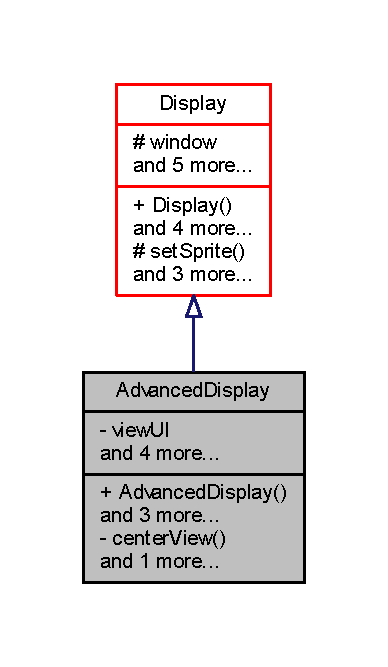
\includegraphics[width=186pt]{class_advanced_display__coll__graph}
\end{center}
\end{figure}
\subsection*{Public Member Functions}
\begin{DoxyCompactItemize}
\item 
\mbox{\Hypertarget{class_advanced_display_a12f2ccc1e24ed1d6d9a68cea1447166f}\label{class_advanced_display_a12f2ccc1e24ed1d6d9a68cea1447166f}} 
{\bfseries Advanced\+Display} (\hyperlink{class_layer}{Layer} $\ast$\+\_\+layer)
\item 
\mbox{\Hypertarget{class_advanced_display_a67925105fd118bb0baf2c92bf13e46c3}\label{class_advanced_display_a67925105fd118bb0baf2c92bf13e46c3}} 
void {\bfseries change\+Scale} (double x, double y)
\item 
\mbox{\Hypertarget{class_advanced_display_a8f1a3ff301cf6261d6c40296d9a926f8}\label{class_advanced_display_a8f1a3ff301cf6261d6c40296d9a926f8}} 
void {\bfseries update} ()
\item 
\mbox{\Hypertarget{class_advanced_display_ae7ce015fcaf05f4a34c123bff64ebb2e}\label{class_advanced_display_ae7ce015fcaf05f4a34c123bff64ebb2e}} 
void {\bfseries handle\+Viewer\+Event} (View\+Events ev)
\end{DoxyCompactItemize}
\subsection*{Private Member Functions}
\begin{DoxyCompactItemize}
\item 
\mbox{\Hypertarget{class_advanced_display_a7bc4ba26e6834551f95769ff6be3da84}\label{class_advanced_display_a7bc4ba26e6834551f95769ff6be3da84}} 
void {\bfseries center\+View} ()
\item 
\mbox{\Hypertarget{class_advanced_display_adaa4a1772d599c5224bf8f0c3476138a}\label{class_advanced_display_adaa4a1772d599c5224bf8f0c3476138a}} 
void {\bfseries change\+Zoom} (bool make\+\_\+closer)
\end{DoxyCompactItemize}
\subsection*{Private Attributes}
\begin{DoxyCompactItemize}
\item 
\mbox{\Hypertarget{class_advanced_display_a1d6b163d432d3a1fa01568fbebd5e496}\label{class_advanced_display_a1d6b163d432d3a1fa01568fbebd5e496}} 
sf\+::\+View {\bfseries view\+UI}
\item 
\mbox{\Hypertarget{class_advanced_display_a77c1ded61c1988f130205e4248f0bd07}\label{class_advanced_display_a77c1ded61c1988f130205e4248f0bd07}} 
sf\+::\+Vector2f {\bfseries max\+\_\+size}
\item 
\mbox{\Hypertarget{class_advanced_display_a5a51a04f2b299f784ec96c9438b84a9d}\label{class_advanced_display_a5a51a04f2b299f784ec96c9438b84a9d}} 
sf\+::\+Vector2f {\bfseries min\+\_\+size}
\item 
\mbox{\Hypertarget{class_advanced_display_a2107d1ad65c137bdf4fe2ebb64cff29c}\label{class_advanced_display_a2107d1ad65c137bdf4fe2ebb64cff29c}} 
double {\bfseries l\+\_\+heigth}
\item 
\mbox{\Hypertarget{class_advanced_display_ae8c55cb678ad26dbbb47b6a837a74886}\label{class_advanced_display_ae8c55cb678ad26dbbb47b6a837a74886}} 
double {\bfseries l\+\_\+width}
\end{DoxyCompactItemize}
\subsection*{Additional Inherited Members}


The documentation for this class was generated from the following files\+:\begin{DoxyCompactItemize}
\item 
Advanced\+Display.\+h\item 
Advanced\+Display.\+cpp\end{DoxyCompactItemize}

\hypertarget{class_auxiliary_layer}{}\section{Auxiliary\+Layer Class Reference}
\label{class_auxiliary_layer}\index{Auxiliary\+Layer@{Auxiliary\+Layer}}


Superstructure class for built-\/in \hyperlink{class_layer}{Layer} classes.  




{\ttfamily \#include $<$Auxiliary\+Layer.\+h$>$}



Collaboration diagram for Auxiliary\+Layer\+:
\nopagebreak
\begin{figure}[H]
\begin{center}
\leavevmode
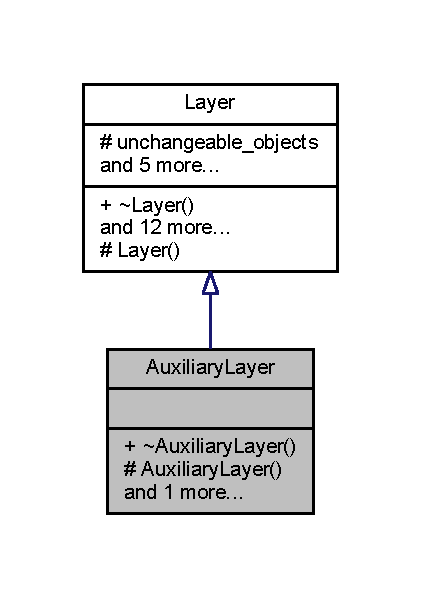
\includegraphics[width=179pt]{class_auxiliary_layer__coll__graph}
\end{center}
\end{figure}
\subsection*{Protected Member Functions}
\begin{DoxyCompactItemize}
\item 
\mbox{\Hypertarget{class_auxiliary_layer_a14a068a62e260548e70859a506a2fe7d}\label{class_auxiliary_layer_a14a068a62e260548e70859a506a2fe7d}} 
\hyperlink{class_auxiliary_layer_a14a068a62e260548e70859a506a2fe7d}{Auxiliary\+Layer} ()
\begin{DoxyCompactList}\small\item\em Default constructor. \end{DoxyCompactList}\item 
virtual bool \hyperlink{class_auxiliary_layer_a2e8e6d2252aa08fc4e329b1301c52908}{is\+Contains} (double x, double y, \hyperlink{class_object}{Object} $\ast$button)
\begin{DoxyCompactList}\small\item\em Check the entry of a coordinate into an object (button default) \end{DoxyCompactList}\end{DoxyCompactItemize}
\subsection*{Additional Inherited Members}


\subsection{Detailed Description}
Superstructure class for built-\/in \hyperlink{class_layer}{Layer} classes. 

\begin{DoxyAuthor}{Author}
Vasily 
\end{DoxyAuthor}
\begin{DoxyVersion}{Version}
1.\+0 
\end{DoxyVersion}
\begin{DoxyDate}{Date}
June 2017
\end{DoxyDate}
Provides functions which necessary for built-\/in \hyperlink{class_layer}{Layer} classes such as main menu, end of the game screen etc. 

\subsection{Member Function Documentation}
\mbox{\Hypertarget{class_auxiliary_layer_a2e8e6d2252aa08fc4e329b1301c52908}\label{class_auxiliary_layer_a2e8e6d2252aa08fc4e329b1301c52908}} 
\index{Auxiliary\+Layer@{Auxiliary\+Layer}!is\+Contains@{is\+Contains}}
\index{is\+Contains@{is\+Contains}!Auxiliary\+Layer@{Auxiliary\+Layer}}
\subsubsection{\texorpdfstring{is\+Contains()}{isContains()}}
{\footnotesize\ttfamily bool Auxiliary\+Layer\+::is\+Contains (\begin{DoxyParamCaption}\item[{double}]{x,  }\item[{double}]{y,  }\item[{\hyperlink{class_object}{Object} $\ast$}]{button }\end{DoxyParamCaption})\hspace{0.3cm}{\ttfamily [protected]}, {\ttfamily [virtual]}}



Check the entry of a coordinate into an object (button default) 


\begin{DoxyParams}{Parameters}
{\em x} & x coordinate \\
\hline
{\em y} & y coordinate \\
\hline
{\em button} & object to check \\
\hline
\end{DoxyParams}


The documentation for this class was generated from the following files\+:\begin{DoxyCompactItemize}
\item 
\hyperlink{_auxiliary_layer_8h}{Auxiliary\+Layer.\+h}\item 
Auxiliary\+Layer.\+cpp\end{DoxyCompactItemize}

\hypertarget{class_bonus}{}\section{Bonus Class Reference}
\label{class_bonus}\index{Bonus@{Bonus}}


Some serum that have an impact to the hero.  




{\ttfamily \#include $<$Bonus.\+h$>$}



Collaboration diagram for Bonus\+:
\nopagebreak
\begin{figure}[H]
\begin{center}
\leavevmode
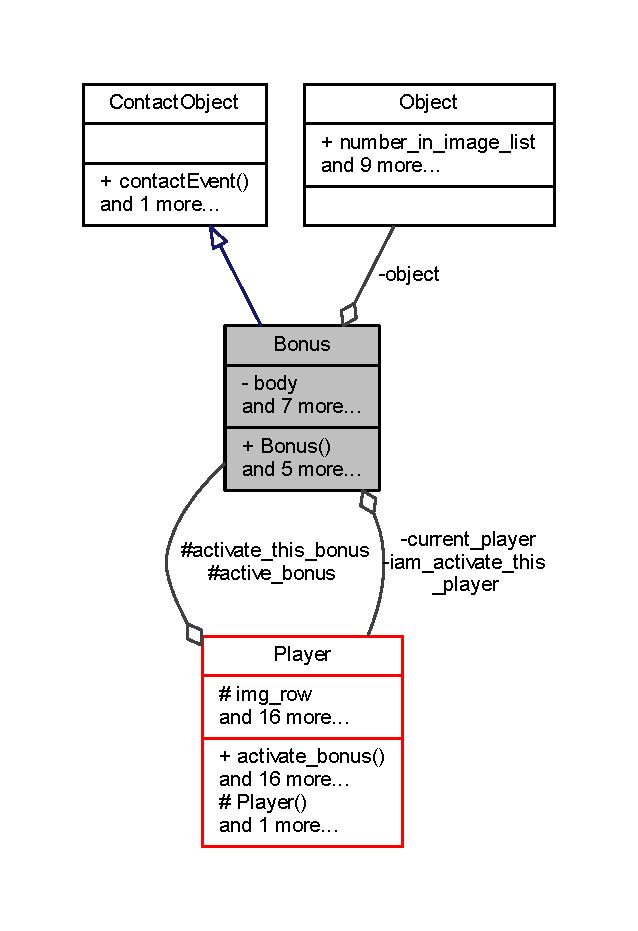
\includegraphics[width=306pt]{class_bonus__coll__graph}
\end{center}
\end{figure}
\subsection*{Public Member Functions}
\begin{DoxyCompactItemize}
\item 
\hyperlink{class_bonus_ac8581e33c82c8d6515b78ccffcf6f11b}{Bonus} (double modificator, double \hyperlink{class_bonus_a7af3e40f87206d34e4689f53e37733b3}{time}, \hyperlink{_bonus_8h_ad6d58ebabfbf9aa4181bfe97a5d8d984}{Bonus\+Type} \hyperlink{class_bonus_a3e8678940c7ea4679428e78874d92117}{bonus\+\_\+type}, \hyperlink{class_player}{Player} $\ast$$\ast$\+\_\+current\+\_\+player, b2\+Body $\ast$\+\_\+body, \hyperlink{class_object}{Object} $\ast$\+\_\+object, std\+::chrono\+::duration$<$ double $>$ $\ast$\hyperlink{class_bonus_a98befe64efce3a1c5c93f2d694ea1abc}{duration})
\begin{DoxyCompactList}\small\item\em Defined constructor for this class. \end{DoxyCompactList}\item 
\hyperlink{class_object}{Object} $\ast$ \hyperlink{class_bonus_a5964466dfbb4b4e3e7d3eafcb9dae7db}{get\+Object} ()
\item 
bool \hyperlink{class_bonus_a78f64b402daa7593afb28b78baf6d15e}{activate} (\hyperlink{class_object}{Object} $\ast$\+\_\+object)
\begin{DoxyCompactList}\small\item\em Apllies the bonus effect. \end{DoxyCompactList}\item 
void \hyperlink{class_bonus_a52875b799a9937f5c398f8f95d9ead98}{deactivate} ()
\begin{DoxyCompactList}\small\item\em Terminates the action of the bonus effect. \end{DoxyCompactList}\item 
\mbox{\Hypertarget{class_bonus_a40703fa50a436a844f0638557a175be0}\label{class_bonus_a40703fa50a436a844f0638557a175be0}} 
void \hyperlink{class_bonus_a40703fa50a436a844f0638557a175be0}{update} ()
\begin{DoxyCompactList}\small\item\em update bonus state (remaining time of impact) \end{DoxyCompactList}\end{DoxyCompactItemize}
\subsection*{Private Member Functions}
\begin{DoxyCompactItemize}
\item 
\mbox{\Hypertarget{class_bonus_abc52e8c896f8ec6631ac5dcd7e4daf12}\label{class_bonus_abc52e8c896f8ec6631ac5dcd7e4daf12}} 
void \hyperlink{class_bonus_abc52e8c896f8ec6631ac5dcd7e4daf12}{contact\+Event} (b2\+Contact $\ast$contact, bool is\+\_\+begin)
\begin{DoxyCompactList}\small\item\em inherited from \hyperlink{class_contact_object}{Contact\+Object} class \end{DoxyCompactList}\end{DoxyCompactItemize}
\subsection*{Private Attributes}
\begin{DoxyCompactItemize}
\item 
\mbox{\Hypertarget{class_bonus_a0c3f3fe18e7d7df28ab12fe2c023d3ff}\label{class_bonus_a0c3f3fe18e7d7df28ab12fe2c023d3ff}} 
b2\+Body $\ast$ \hyperlink{class_bonus_a0c3f3fe18e7d7df28ab12fe2c023d3ff}{body}
\begin{DoxyCompactList}\small\item\em pointer to the box2d body assigned to this bonus \end{DoxyCompactList}\item 
\mbox{\Hypertarget{class_bonus_a7493d5e3afda12e197c5505a66a1c7a1}\label{class_bonus_a7493d5e3afda12e197c5505a66a1c7a1}} 
\hyperlink{class_object}{Object} $\ast$ \hyperlink{class_bonus_a7493d5e3afda12e197c5505a66a1c7a1}{object}
\begin{DoxyCompactList}\small\item\em pointer to the \hyperlink{class_object}{Object} class assigned to this bonus \end{DoxyCompactList}\item 
\mbox{\Hypertarget{class_bonus_a5c03f6529a87fd393efaedb0db7e8b49}\label{class_bonus_a5c03f6529a87fd393efaedb0db7e8b49}} 
\hyperlink{class_player}{Player} $\ast$ \hyperlink{class_bonus_a5c03f6529a87fd393efaedb0db7e8b49}{iam\+\_\+activate\+\_\+this\+\_\+player}
\begin{DoxyCompactList}\small\item\em pointer to the \hyperlink{class_player}{Player} class to which bonus has been applied \end{DoxyCompactList}\item 
\mbox{\Hypertarget{class_bonus_ad5b0534727679d924f60eeaef2ac988d}\label{class_bonus_ad5b0534727679d924f60eeaef2ac988d}} 
\hyperlink{class_player}{Player} $\ast$$\ast$ \hyperlink{class_bonus_ad5b0534727679d924f60eeaef2ac988d}{current\+\_\+player}
\begin{DoxyCompactList}\small\item\em pointer to the pointer containing infofmation about current active hero \end{DoxyCompactList}\item 
\mbox{\Hypertarget{class_bonus_a4a5cd25b27a40406d018e1e3e651d21f}\label{class_bonus_a4a5cd25b27a40406d018e1e3e651d21f}} 
double \hyperlink{class_bonus_a4a5cd25b27a40406d018e1e3e651d21f}{time\+\_\+interval}
\begin{DoxyCompactList}\small\item\em duration of the impact \end{DoxyCompactList}\item 
\mbox{\Hypertarget{class_bonus_a7af3e40f87206d34e4689f53e37733b3}\label{class_bonus_a7af3e40f87206d34e4689f53e37733b3}} 
double \hyperlink{class_bonus_a7af3e40f87206d34e4689f53e37733b3}{time}
\begin{DoxyCompactList}\small\item\em current time that has passed from the begin of the bonus application \end{DoxyCompactList}\item 
\mbox{\Hypertarget{class_bonus_a55548c98a8969d5994fbbcbdd6f35752}\label{class_bonus_a55548c98a8969d5994fbbcbdd6f35752}} 
double \hyperlink{class_bonus_a55548c98a8969d5994fbbcbdd6f35752}{bonus\+\_\+modificator}
\begin{DoxyCompactList}\small\item\em power of the impact \end{DoxyCompactList}\item 
\mbox{\Hypertarget{class_bonus_a3e8678940c7ea4679428e78874d92117}\label{class_bonus_a3e8678940c7ea4679428e78874d92117}} 
\hyperlink{_bonus_8h_ad6d58ebabfbf9aa4181bfe97a5d8d984}{Bonus\+Type} \hyperlink{class_bonus_a3e8678940c7ea4679428e78874d92117}{bonus\+\_\+type}
\begin{DoxyCompactList}\small\item\em bonuse type (see enum Bonus\+Type) \end{DoxyCompactList}\item 
\mbox{\Hypertarget{class_bonus_a07620733fe137be73855a2ac4353771c}\label{class_bonus_a07620733fe137be73855a2ac4353771c}} 
std\+::chrono\+::seconds \hyperlink{class_bonus_a07620733fe137be73855a2ac4353771c}{dts}
\begin{DoxyCompactList}\small\item\em chrono service information \end{DoxyCompactList}\item 
\mbox{\Hypertarget{class_bonus_a98befe64efce3a1c5c93f2d694ea1abc}\label{class_bonus_a98befe64efce3a1c5c93f2d694ea1abc}} 
std\+::chrono\+::duration$<$ double $>$ $\ast$ \hyperlink{class_bonus_a98befe64efce3a1c5c93f2d694ea1abc}{duration}
\begin{DoxyCompactList}\small\item\em pointer to the variable containing information about level time \end{DoxyCompactList}\item 
\mbox{\Hypertarget{class_bonus_a288adde51bbfb1c9a22fc0cad3e5e8b0}\label{class_bonus_a288adde51bbfb1c9a22fc0cad3e5e8b0}} 
std\+::chrono\+::duration$<$ double $>$ \hyperlink{class_bonus_a288adde51bbfb1c9a22fc0cad3e5e8b0}{start}
\begin{DoxyCompactList}\small\item\em chrono start of impact \end{DoxyCompactList}\end{DoxyCompactItemize}


\subsection{Detailed Description}
Some serum that have an impact to the hero. 

\begin{DoxyAuthor}{Author}
Vasily 
\end{DoxyAuthor}
\begin{DoxyVersion}{Version}
1.\+0 
\end{DoxyVersion}
\begin{DoxyDate}{Date}
June 2017 
\end{DoxyDate}


\subsection{Constructor \& Destructor Documentation}
\mbox{\Hypertarget{class_bonus_ac8581e33c82c8d6515b78ccffcf6f11b}\label{class_bonus_ac8581e33c82c8d6515b78ccffcf6f11b}} 
\index{Bonus@{Bonus}!Bonus@{Bonus}}
\index{Bonus@{Bonus}!Bonus@{Bonus}}
\subsubsection{\texorpdfstring{Bonus()}{Bonus()}}
{\footnotesize\ttfamily Bonus\+::\+Bonus (\begin{DoxyParamCaption}\item[{double}]{modificator,  }\item[{double}]{time,  }\item[{\hyperlink{_bonus_8h_ad6d58ebabfbf9aa4181bfe97a5d8d984}{Bonus\+Type}}]{bonus\+\_\+type,  }\item[{\hyperlink{class_player}{Player} $\ast$$\ast$}]{\+\_\+current\+\_\+player,  }\item[{b2\+Body $\ast$}]{\+\_\+body,  }\item[{\hyperlink{class_object}{Object} $\ast$}]{\+\_\+object,  }\item[{std\+::chrono\+::duration$<$ double $>$ $\ast$}]{duration }\end{DoxyParamCaption})}



Defined constructor for this class. 


\begin{DoxyParams}{Parameters}
{\em modificator} & power of the impact \\
\hline
{\em time} & duration of the impact \\
\hline
{\em bonus\+\_\+type} & bonuse type (see enum Bonus\+Type) \\
\hline
{\em \+\_\+current\+\_\+player} & pointer to the pointer containing infofmation about current active hero \\
\hline
{\em \+\_\+body} & pointer to the box2d body assigned to this bonus \\
\hline
{\em \+\_\+object} & pointer to the \hyperlink{class_object}{Object} class assigned to this bonus \\
\hline
{\em duration} & pointer to the variable containing information about level time \\
\hline
\end{DoxyParams}


\subsection{Member Function Documentation}
\mbox{\Hypertarget{class_bonus_a78f64b402daa7593afb28b78baf6d15e}\label{class_bonus_a78f64b402daa7593afb28b78baf6d15e}} 
\index{Bonus@{Bonus}!activate@{activate}}
\index{activate@{activate}!Bonus@{Bonus}}
\subsubsection{\texorpdfstring{activate()}{activate()}}
{\footnotesize\ttfamily bool Bonus\+::activate (\begin{DoxyParamCaption}\item[{\hyperlink{class_object}{Object} $\ast$}]{\+\_\+object }\end{DoxyParamCaption})}



Apllies the bonus effect. 

Delete the image of bonus from the screen and move it to hero ui bonus-\/cell 
\begin{DoxyParams}{Parameters}
{\em \+\_\+object} & pointer to \hyperlink{class_object}{Object} class which define ui bonus-\/cell \\
\hline
\end{DoxyParams}
\mbox{\Hypertarget{class_bonus_a52875b799a9937f5c398f8f95d9ead98}\label{class_bonus_a52875b799a9937f5c398f8f95d9ead98}} 
\index{Bonus@{Bonus}!deactivate@{deactivate}}
\index{deactivate@{deactivate}!Bonus@{Bonus}}
\subsubsection{\texorpdfstring{deactivate()}{deactivate()}}
{\footnotesize\ttfamily void Bonus\+::deactivate (\begin{DoxyParamCaption}{ }\end{DoxyParamCaption})}



Terminates the action of the bonus effect. 

Delete the image of bonus from the hero ui bonus-\/cell \mbox{\Hypertarget{class_bonus_a5964466dfbb4b4e3e7d3eafcb9dae7db}\label{class_bonus_a5964466dfbb4b4e3e7d3eafcb9dae7db}} 
\index{Bonus@{Bonus}!get\+Object@{get\+Object}}
\index{get\+Object@{get\+Object}!Bonus@{Bonus}}
\subsubsection{\texorpdfstring{get\+Object()}{getObject()}}
{\footnotesize\ttfamily \hyperlink{class_object}{Object} $\ast$ Bonus\+::get\+Object (\begin{DoxyParamCaption}{ }\end{DoxyParamCaption})}

\begin{DoxyReturn}{Returns}
pointer to the \hyperlink{class_object}{Object} class assigned to this bonus or bonus-\/cell 
\end{DoxyReturn}


The documentation for this class was generated from the following files\+:\begin{DoxyCompactItemize}
\item 
\hyperlink{_bonus_8h}{Bonus.\+h}\item 
Bonus.\+cpp\end{DoxyCompactItemize}

\hypertarget{class_contact_object}{}\section{Contact\+Object Class Reference}
\label{class_contact_object}\index{Contact\+Object@{Contact\+Object}}


Interface for an object which can collide with another in box2d world.  




{\ttfamily \#include $<$Contact\+Object.\+h$>$}



Collaboration diagram for Contact\+Object\+:\nopagebreak
\begin{figure}[H]
\begin{center}
\leavevmode
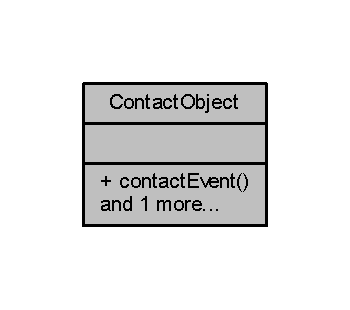
\includegraphics[width=168pt]{class_contact_object__coll__graph}
\end{center}
\end{figure}
\subsection*{Public Member Functions}
\begin{DoxyCompactItemize}
\item 
virtual void \hyperlink{class_contact_object_a53d2dfc1d9c2821e9c62e80ce62a6435}{contact\+Event} (b2\+Contact $\ast$contact, bool is\+Begin)=0
\begin{DoxyCompactList}\small\item\em Define object reaction to the collision in box2d world. \end{DoxyCompactList}\end{DoxyCompactItemize}


\subsection{Detailed Description}
Interface for an object which can collide with another in box2d world. 

\begin{DoxyAuthor}{Author}
Vasily 
\end{DoxyAuthor}
\begin{DoxyVersion}{Version}
1.\+0 
\end{DoxyVersion}
\begin{DoxyDate}{Date}
June 2017 
\end{DoxyDate}


\subsection{Member Function Documentation}
\mbox{\Hypertarget{class_contact_object_a53d2dfc1d9c2821e9c62e80ce62a6435}\label{class_contact_object_a53d2dfc1d9c2821e9c62e80ce62a6435}} 
\index{Contact\+Object@{Contact\+Object}!contact\+Event@{contact\+Event}}
\index{contact\+Event@{contact\+Event}!Contact\+Object@{Contact\+Object}}
\subsubsection{\texorpdfstring{contact\+Event()}{contactEvent()}}
{\footnotesize\ttfamily virtual void Contact\+Object\+::contact\+Event (\begin{DoxyParamCaption}\item[{b2\+Contact $\ast$}]{contact,  }\item[{bool}]{is\+Begin }\end{DoxyParamCaption})\hspace{0.3cm}{\ttfamily [pure virtual]}}



Define object reaction to the collision in box2d world. 


\begin{DoxyParams}{Parameters}
{\em contact} & pointer to box2d b2\+Contact class \\
\hline
{\em is\+Begin} & \textquotesingle{}false\textquotesingle{} -\/ end of the collision; \textquotesingle{}true\textquotesingle{} -\/ start of the collision \\
\hline
\end{DoxyParams}


Implemented in \hyperlink{class_player_sensor_a6977b8699ebf0d3d2d2b177665060f21}{Player\+Sensor}, \hyperlink{class_bonus_a903865168ff7fd91e0e2de23f849c553}{Bonus}, \hyperlink{class_non_static_obj_ae129119384cf9df2b7b1a7849b6112de}{Non\+Static\+Obj}, \hyperlink{class_danger_object_aebfc6b5b3dc2452cae78b157a29e8824}{Danger\+Object}, \hyperlink{class_lever_a9ec153b4c960d0a187539cc8f07e5bd9}{Lever}, \hyperlink{class_sensor_a08bfa36c84277677f3bd5fb14127fca7}{Sensor}, \hyperlink{class_final_a9ebc21296dd28e993f2ee8cbb47a3b37}{Final}, and \hyperlink{class_visible_sensor_a63bcb9da7556a6356cca3b08f7808bd8}{Visible\+Sensor}.



The documentation for this class was generated from the following file\+:\begin{DoxyCompactItemize}
\item 
\hyperlink{_contact_object_8h}{Contact\+Object.\+h}\end{DoxyCompactItemize}

\hypertarget{class_controller}{}\section{Controller Class Reference}
\label{class_controller}\index{Controller@{Controller}}


Operating element in M\+VC structure.  




{\ttfamily \#include $<$Controller.\+h$>$}



Collaboration diagram for Controller\+:\nopagebreak
\begin{figure}[H]
\begin{center}
\leavevmode
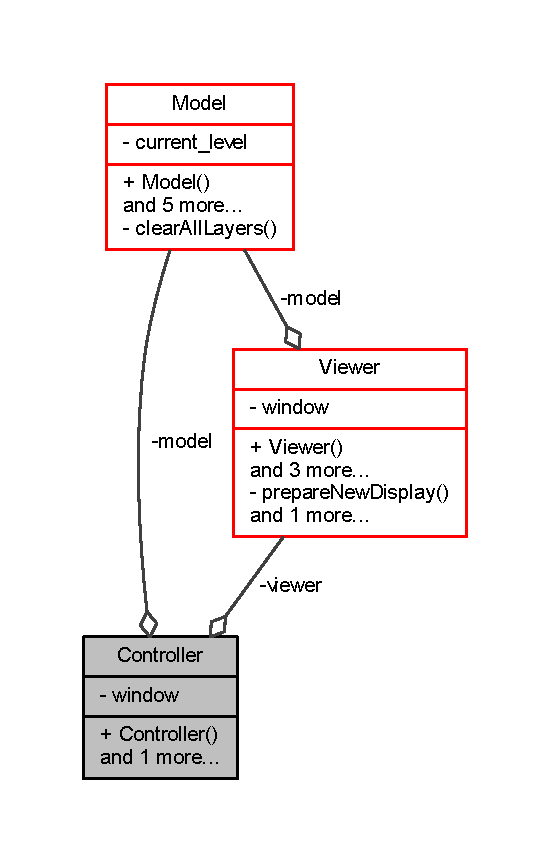
\includegraphics[width=264pt]{class_controller__coll__graph}
\end{center}
\end{figure}
\subsection*{Public Member Functions}
\begin{DoxyCompactItemize}
\item 
\hyperlink{class_controller_ae2231c787d852af79c95433cf30cbe9f}{Controller} (\hyperlink{class_model}{Model} $\ast$\+\_\+model, \hyperlink{class_viewer}{Viewer} $\ast$\+\_\+viewer)
\begin{DoxyCompactList}\small\item\em Defined constructor for this class. \end{DoxyCompactList}\item 
\mbox{\Hypertarget{class_controller_a6ebc30e3213a87318b8f6d7c7f2edc7c}\label{class_controller_a6ebc30e3213a87318b8f6d7c7f2edc7c}} 
void \hyperlink{class_controller_a6ebc30e3213a87318b8f6d7c7f2edc7c}{observe} ()
\begin{DoxyCompactList}\small\item\em Start the game life cycle. \end{DoxyCompactList}\end{DoxyCompactItemize}
\subsection*{Private Attributes}
\begin{DoxyCompactItemize}
\item 
\mbox{\Hypertarget{class_controller_a9c31118fa8ad5b061deae97b57fadbec}\label{class_controller_a9c31118fa8ad5b061deae97b57fadbec}} 
sf\+::\+Render\+Window $\ast$ \hyperlink{class_controller_a9c31118fa8ad5b061deae97b57fadbec}{window}
\begin{DoxyCompactList}\small\item\em Pointer to the instance window of the game. \end{DoxyCompactList}\item 
\mbox{\Hypertarget{class_controller_a6f6ea54052742d3940adfcfce885bae9}\label{class_controller_a6f6ea54052742d3940adfcfce885bae9}} 
\hyperlink{class_model}{Model} $\ast$ \hyperlink{class_controller_a6f6ea54052742d3940adfcfce885bae9}{model}
\begin{DoxyCompactList}\small\item\em Pointer to the \hyperlink{class_model}{Model} class. \end{DoxyCompactList}\item 
\mbox{\Hypertarget{class_controller_a81f966e6dcf07b90a15453ee54945182}\label{class_controller_a81f966e6dcf07b90a15453ee54945182}} 
\hyperlink{class_viewer}{Viewer} $\ast$ \hyperlink{class_controller_a81f966e6dcf07b90a15453ee54945182}{viewer}
\begin{DoxyCompactList}\small\item\em Pointer to the \hyperlink{class_viewer}{Viewer} class. \end{DoxyCompactList}\end{DoxyCompactItemize}


\subsection{Detailed Description}
Operating element in M\+VC structure. 

\begin{DoxyAuthor}{Author}
Vasily 
\end{DoxyAuthor}
\begin{DoxyVersion}{Version}
1.\+0 
\end{DoxyVersion}
\begin{DoxyDate}{Date}
June 2017
\end{DoxyDate}
Processes S\+F\+M\+L-\/window events and provides communication between \hyperlink{class_viewer}{Viewer} and \hyperlink{class_model}{Model} classes 

\subsection{Constructor \& Destructor Documentation}
\mbox{\Hypertarget{class_controller_ae2231c787d852af79c95433cf30cbe9f}\label{class_controller_ae2231c787d852af79c95433cf30cbe9f}} 
\index{Controller@{Controller}!Controller@{Controller}}
\index{Controller@{Controller}!Controller@{Controller}}
\subsubsection{\texorpdfstring{Controller()}{Controller()}}
{\footnotesize\ttfamily Controller\+::\+Controller (\begin{DoxyParamCaption}\item[{\hyperlink{class_model}{Model} $\ast$}]{\+\_\+model,  }\item[{\hyperlink{class_viewer}{Viewer} $\ast$}]{\+\_\+viewer }\end{DoxyParamCaption})}



Defined constructor for this class. 


\begin{DoxyParams}{Parameters}
{\em \+\_\+model} & pointer to the \hyperlink{class_model}{Model} class, which will use in M\+VC model \\
\hline
{\em \+\_\+viewer} & pointer to the \hyperlink{class_viewer}{Viewer} class, which will use in M\+VC model \\
\hline
\end{DoxyParams}


The documentation for this class was generated from the following files\+:\begin{DoxyCompactItemize}
\item 
\hyperlink{_controller_8h}{Controller.\+h}\item 
Controller.\+cpp\end{DoxyCompactItemize}

\hypertarget{class_danger_object}{}\section{Danger\+Object Class Reference}
\label{class_danger_object}\index{Danger\+Object@{Danger\+Object}}


Danger entity that can be assigned to the platform.  




{\ttfamily \#include $<$Danger\+Object.\+h$>$}



Collaboration diagram for Danger\+Object\+:
\nopagebreak
\begin{figure}[H]
\begin{center}
\leavevmode
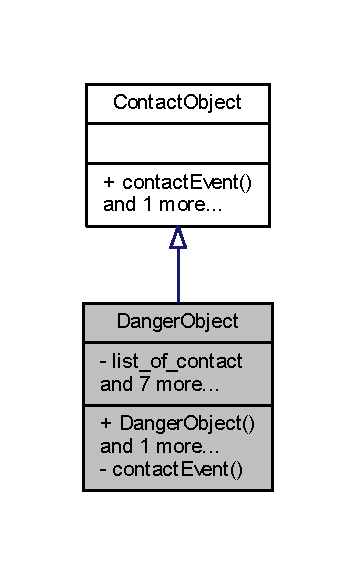
\includegraphics[width=298pt]{class_danger_object__coll__graph}
\end{center}
\end{figure}
\subsection*{Public Member Functions}
\begin{DoxyCompactItemize}
\item 
\hyperlink{class_danger_object_a87186516066d7d47dcea87eec44ee616}{Danger\+Object} (std\+::list$<$ b2\+Body $\ast$$>$ \+\_\+boundaries, double \+\_\+damage, b2\+Body $\ast$body, std\+::chrono\+::duration$<$ double $>$ $\ast$\+\_\+duration)
\begin{DoxyCompactList}\small\item\em Defined constructor for this class. \end{DoxyCompactList}\item 
\mbox{\Hypertarget{class_danger_object_a0c058336c21ee3e9b8fca876adda2dda}\label{class_danger_object_a0c058336c21ee3e9b8fca876adda2dda}} 
void \hyperlink{class_danger_object_a0c058336c21ee3e9b8fca876adda2dda}{update} ()
\begin{DoxyCompactList}\small\item\em update bonus state (should it to make damage or not) \end{DoxyCompactList}\end{DoxyCompactItemize}
\subsection*{Private Member Functions}
\begin{DoxyCompactItemize}
\item 
\mbox{\Hypertarget{class_danger_object_a542702fda89ff9549866d9b93a603fbb}\label{class_danger_object_a542702fda89ff9549866d9b93a603fbb}} 
void \hyperlink{class_danger_object_a542702fda89ff9549866d9b93a603fbb}{contact\+Event} (b2\+Contact $\ast$contact, bool is\+\_\+begin)
\begin{DoxyCompactList}\small\item\em inherited from \hyperlink{class_contact_object}{Contact\+Object} class \end{DoxyCompactList}\end{DoxyCompactItemize}
\subsection*{Private Attributes}
\begin{DoxyCompactItemize}
\item 
\mbox{\Hypertarget{class_danger_object_a3b032f295d584177435e4ee71e8a0647}\label{class_danger_object_a3b032f295d584177435e4ee71e8a0647}} 
std\+::vector$<$ \hyperlink{class_player}{Player} $\ast$ $>$ \hyperlink{class_danger_object_a3b032f295d584177435e4ee71e8a0647}{list\+\_\+of\+\_\+contact}
\begin{DoxyCompactList}\small\item\em list of players which have contact with this danger object \end{DoxyCompactList}\item 
\mbox{\Hypertarget{class_danger_object_a81602fd52def64c26dd7ae488d523111}\label{class_danger_object_a81602fd52def64c26dd7ae488d523111}} 
double \hyperlink{class_danger_object_a81602fd52def64c26dd7ae488d523111}{damage}
\begin{DoxyCompactList}\small\item\em power of the damage (health\+\_\+loss) \end{DoxyCompactList}\item 
\mbox{\Hypertarget{class_danger_object_a1a5e8ba303583a6a1dae79b218e07f6f}\label{class_danger_object_a1a5e8ba303583a6a1dae79b218e07f6f}} 
double \hyperlink{class_danger_object_a1a5e8ba303583a6a1dae79b218e07f6f}{time\+\_\+interval}
\begin{DoxyCompactList}\small\item\em duration of the time intervals with which the damage will be applied \end{DoxyCompactList}\item 
\mbox{\Hypertarget{class_danger_object_a47bc7031c9d5afd3dffc902e464e6911}\label{class_danger_object_a47bc7031c9d5afd3dffc902e464e6911}} 
double \hyperlink{class_danger_object_a47bc7031c9d5afd3dffc902e464e6911}{time}
\begin{DoxyCompactList}\small\item\em current time that has passed from the begin of the bonus application \end{DoxyCompactList}\item 
\mbox{\Hypertarget{class_danger_object_a2cb289f3bf483c5e73282342ced2bd77}\label{class_danger_object_a2cb289f3bf483c5e73282342ced2bd77}} 
std\+::chrono\+::milliseconds \hyperlink{class_danger_object_a2cb289f3bf483c5e73282342ced2bd77}{dts}
\begin{DoxyCompactList}\small\item\em chrono service information \end{DoxyCompactList}\item 
\mbox{\Hypertarget{class_danger_object_a4bb9e8dffdc1815094e867824ea4e393}\label{class_danger_object_a4bb9e8dffdc1815094e867824ea4e393}} 
std\+::chrono\+::duration$<$ double $>$ $\ast$ \hyperlink{class_danger_object_a4bb9e8dffdc1815094e867824ea4e393}{duration}
\begin{DoxyCompactList}\small\item\em pointer to the variable containing information about level time \end{DoxyCompactList}\item 
\mbox{\Hypertarget{class_danger_object_aa56801b799fc9193bb3ae64c400aa614}\label{class_danger_object_aa56801b799fc9193bb3ae64c400aa614}} 
std\+::chrono\+::duration$<$ double $>$ \hyperlink{class_danger_object_aa56801b799fc9193bb3ae64c400aa614}{start}
\begin{DoxyCompactList}\small\item\em chrono start of impact \end{DoxyCompactList}\end{DoxyCompactItemize}


\subsection{Detailed Description}
Danger entity that can be assigned to the platform. 

\begin{DoxyAuthor}{Author}
Vasily 
\end{DoxyAuthor}
\begin{DoxyVersion}{Version}
1.\+0 
\end{DoxyVersion}
\begin{DoxyDate}{Date}
June 2017 
\end{DoxyDate}


\subsection{Constructor \& Destructor Documentation}
\mbox{\Hypertarget{class_danger_object_a87186516066d7d47dcea87eec44ee616}\label{class_danger_object_a87186516066d7d47dcea87eec44ee616}} 
\index{Danger\+Object@{Danger\+Object}!Danger\+Object@{Danger\+Object}}
\index{Danger\+Object@{Danger\+Object}!Danger\+Object@{Danger\+Object}}
\subsubsection{\texorpdfstring{Danger\+Object()}{DangerObject()}}
{\footnotesize\ttfamily Danger\+Object\+::\+Danger\+Object (\begin{DoxyParamCaption}\item[{std\+::list$<$ b2\+Body $\ast$$>$}]{\+\_\+boundaries,  }\item[{double}]{\+\_\+damage,  }\item[{b2\+Body $\ast$}]{body,  }\item[{std\+::chrono\+::duration$<$ double $>$ $\ast$}]{\+\_\+duration }\end{DoxyParamCaption})}



Defined constructor for this class. 


\begin{DoxyParams}{Parameters}
{\em \+\_\+boundaries} & list of pointer to the sensors which stick to this danger object \\
\hline
{\em \+\_\+damage} & power of the damage (health\+\_\+loss) \\
\hline
{\em body} & pointer to the box2d body assigned to this danger object \\
\hline
{\em \+\_\+duration} & pointer to the variable containing information about level time \\
\hline
\end{DoxyParams}


The documentation for this class was generated from the following files\+:\begin{DoxyCompactItemize}
\item 
\hyperlink{_danger_object_8h}{Danger\+Object.\+h}\item 
Danger\+Object.\+cpp\end{DoxyCompactItemize}

\hypertarget{class_dexterous_player}{}\section{Dexterous\+Player Class Reference}
\label{class_dexterous_player}\index{Dexterous\+Player@{Dexterous\+Player}}


Contains information about dexterous characret.  




{\ttfamily \#include $<$Dexterous\+Player.\+h$>$}



Collaboration diagram for Dexterous\+Player\+:\nopagebreak
\begin{figure}[H]
\begin{center}
\leavevmode
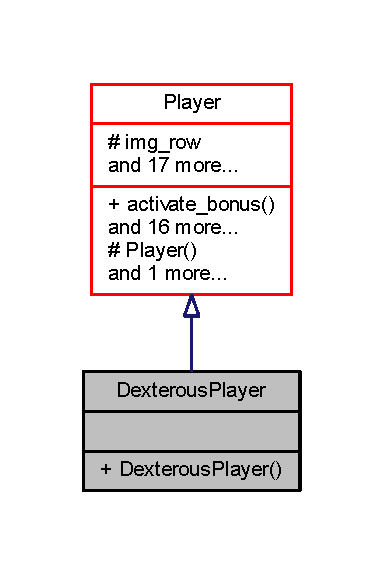
\includegraphics[width=184pt]{class_dexterous_player__coll__graph}
\end{center}
\end{figure}
\subsection*{Public Member Functions}
\begin{DoxyCompactItemize}
\item 
\hyperlink{class_dexterous_player_a852e50ce93cf01a9b042e58a6bcf2e4e}{Dexterous\+Player} (int \+\_\+level\+\_\+width, int \+\_\+level\+\_\+height, b2\+Body $\ast$\+\_\+body, \hyperlink{class_object}{Object} $\ast$\+\_\+object, int \+\_\+health, Return\+Events $\ast$\+\_\+re)
\begin{DoxyCompactList}\small\item\em Defined constructor for this class. \end{DoxyCompactList}\end{DoxyCompactItemize}
\subsection*{Additional Inherited Members}


\subsection{Detailed Description}
Contains information about dexterous characret. 

\begin{DoxyAuthor}{Author}
Vasily 
\end{DoxyAuthor}
\begin{DoxyVersion}{Version}
1.\+0 
\end{DoxyVersion}
\begin{DoxyDate}{Date}
June 2017 
\end{DoxyDate}


\subsection{Constructor \& Destructor Documentation}
\mbox{\Hypertarget{class_dexterous_player_a852e50ce93cf01a9b042e58a6bcf2e4e}\label{class_dexterous_player_a852e50ce93cf01a9b042e58a6bcf2e4e}} 
\index{Dexterous\+Player@{Dexterous\+Player}!Dexterous\+Player@{Dexterous\+Player}}
\index{Dexterous\+Player@{Dexterous\+Player}!Dexterous\+Player@{Dexterous\+Player}}
\subsubsection{\texorpdfstring{Dexterous\+Player()}{DexterousPlayer()}}
{\footnotesize\ttfamily Dexterous\+Player\+::\+Dexterous\+Player (\begin{DoxyParamCaption}\item[{int}]{\+\_\+level\+\_\+width,  }\item[{int}]{\+\_\+level\+\_\+height,  }\item[{b2\+Body $\ast$}]{\+\_\+body,  }\item[{\hyperlink{class_object}{Object} $\ast$}]{\+\_\+object,  }\item[{int}]{\+\_\+health,  }\item[{Return\+Events $\ast$}]{\+\_\+re }\end{DoxyParamCaption})}



Defined constructor for this class. 


\begin{DoxyParams}{Parameters}
{\em \+\_\+level\+\_\+width} & the width in pixels of this level \\
\hline
{\em \+\_\+level\+\_\+height} & the height in pixels of this level \\
\hline
{\em \+\_\+body} & pointer to the box2d body assigned to this character \\
\hline
{\em \+\_\+object} & pointer to the \hyperlink{class_object}{Object} class assigned to this character \\
\hline
{\em \+\_\+health} & the maximum level of health reserve for this caracter \\
\hline
{\em \+\_\+re} & pointer to the variable which contains reply of the current level during last iteration (see \hyperlink{class_layer}{Layer} class) \\
\hline
\end{DoxyParams}


The documentation for this class was generated from the following files\+:\begin{DoxyCompactItemize}
\item 
\hyperlink{_dexterous_player_8h}{Dexterous\+Player.\+h}\item 
Dexterous\+Player.\+cpp\end{DoxyCompactItemize}

\hypertarget{class_display}{}\section{Display Class Reference}
\label{class_display}\index{Display@{Display}}


Provides a display for \hyperlink{class_layer}{Layer} information.  




{\ttfamily \#include $<$Display.\+h$>$}



Collaboration diagram for Display\+:
\nopagebreak
\begin{figure}[H]
\begin{center}
\leavevmode
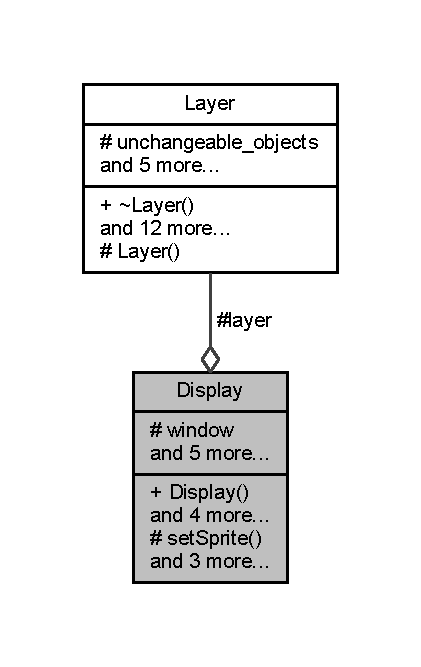
\includegraphics[width=350pt]{class_display__coll__graph}
\end{center}
\end{figure}
\subsection*{Public Member Functions}
\begin{DoxyCompactItemize}
\item 
\hyperlink{class_display_a26d0e334f62107584f42e8fa3608f546}{Display} (\hyperlink{class_layer}{Layer} $\ast$\+\_\+layer)
\begin{DoxyCompactList}\small\item\em Defined constructor for this class. \end{DoxyCompactList}\item 
\mbox{\Hypertarget{class_display_ab4a3db38f39ad17537c58cbd17bc0d04}\label{class_display_ab4a3db38f39ad17537c58cbd17bc0d04}} 
virtual void \hyperlink{class_display_ab4a3db38f39ad17537c58cbd17bc0d04}{change\+Scale} ()
\begin{DoxyCompactList}\small\item\em change scale of the screen \end{DoxyCompactList}\item 
virtual void \hyperlink{class_display_a0383047ebb0be089fe56826e84f9fcf1}{handle\+Viewer\+Event} (\hyperlink{_events_8h_a7e30376069ab6f940d101ae67eb3fb34}{View\+Events} event)
\begin{DoxyCompactList}\small\item\em provide display reaction on user action and model changes (command from \hyperlink{class_controller}{Controller}) \end{DoxyCompactList}\item 
\mbox{\Hypertarget{class_display_ad2740b779d61e461c4dcaaf34f1fcd8f}\label{class_display_ad2740b779d61e461c4dcaaf34f1fcd8f}} 
virtual void \hyperlink{class_display_ad2740b779d61e461c4dcaaf34f1fcd8f}{update} ()
\begin{DoxyCompactList}\small\item\em update information on the screen \end{DoxyCompactList}\end{DoxyCompactItemize}
\subsection*{Protected Member Functions}
\begin{DoxyCompactItemize}
\item 
sf\+::\+Sprite \hyperlink{class_display_aadebd92927d32d9766bc2d7bfff272f3}{set\+Sprite} (\hyperlink{class_object}{Object} it)
\begin{DoxyCompactList}\small\item\em internal function which fill sfml sprite with information from \hyperlink{class_object}{Object} class \end{DoxyCompactList}\item 
sf\+::\+Sprite \hyperlink{class_display_ad7ab55961c0e45e5f4f3caddd9359b1b}{set\+Dynamic\+Sprite} (\hyperlink{class_object}{Object} it)
\begin{DoxyCompactList}\small\item\em internal function which fill sfml sprite with information from \hyperlink{class_object}{Object} class \end{DoxyCompactList}\item 
\mbox{\Hypertarget{class_display_ad0ff309e86415292e5b62e28ee658407}\label{class_display_ad0ff309e86415292e5b62e28ee658407}} 
void \hyperlink{class_display_ad0ff309e86415292e5b62e28ee658407}{load\+Display} ()
\begin{DoxyCompactList}\small\item\em prepare class for work \end{DoxyCompactList}\item 
\mbox{\Hypertarget{class_display_a316e10fdc05529ec6d73f6a82aedbf3a}\label{class_display_a316e10fdc05529ec6d73f6a82aedbf3a}} 
void \hyperlink{class_display_a316e10fdc05529ec6d73f6a82aedbf3a}{update\+Without\+Text} ()
\begin{DoxyCompactList}\small\item\em special update without text information (which doesn\textquotesingle{}t display) \end{DoxyCompactList}\end{DoxyCompactItemize}
\subsection*{Protected Attributes}
\begin{DoxyCompactItemize}
\item 
\mbox{\Hypertarget{class_display_a78cd676fe244dad818b5567367fdfb33}\label{class_display_a78cd676fe244dad818b5567367fdfb33}} 
\hyperlink{class_layer}{Layer} $\ast$ \hyperlink{class_display_a78cd676fe244dad818b5567367fdfb33}{layer}
\begin{DoxyCompactList}\small\item\em pointer to the \hyperlink{class_layer}{Layer} with model information to display \end{DoxyCompactList}\item 
\mbox{\Hypertarget{class_display_ab2bec26675f5903449716d95bb0107bd}\label{class_display_ab2bec26675f5903449716d95bb0107bd}} 
sf\+::\+Render\+Window $\ast$ \hyperlink{class_display_ab2bec26675f5903449716d95bb0107bd}{window}
\begin{DoxyCompactList}\small\item\em pointer to the singletone application window \end{DoxyCompactList}\item 
\mbox{\Hypertarget{class_display_ad84f83c5fd704ce49ac3f038f07ae6dd}\label{class_display_ad84f83c5fd704ce49ac3f038f07ae6dd}} 
sf\+::\+View \hyperlink{class_display_ad84f83c5fd704ce49ac3f038f07ae6dd}{view}
\begin{DoxyCompactList}\small\item\em base view for elements at the level \end{DoxyCompactList}\item 
\mbox{\Hypertarget{class_display_a2c39b9f00cdfb5f4114c5a40e8af076d}\label{class_display_a2c39b9f00cdfb5f4114c5a40e8af076d}} 
sf\+::\+Font \hyperlink{class_display_a2c39b9f00cdfb5f4114c5a40e8af076d}{font}
\begin{DoxyCompactList}\small\item\em text font \end{DoxyCompactList}\item 
\mbox{\Hypertarget{class_display_a8369eaf8bd4706d966c7e1be78d061fe}\label{class_display_a8369eaf8bd4706d966c7e1be78d061fe}} 
sf\+::\+Text \hyperlink{class_display_a8369eaf8bd4706d966c7e1be78d061fe}{text}
\begin{DoxyCompactList}\small\item\em sfml text container \end{DoxyCompactList}\item 
\mbox{\Hypertarget{class_display_a1a3dd88f53281f8bc2294f33862dced0}\label{class_display_a1a3dd88f53281f8bc2294f33862dced0}} 
std\+::vector$<$ sf\+::\+Sprite $>$ \hyperlink{class_display_a1a3dd88f53281f8bc2294f33862dced0}{constant\+\_\+sprite}
\begin{DoxyCompactList}\small\item\em vector containing sfml sprites for non-\/changeable elements \end{DoxyCompactList}\item 
\mbox{\Hypertarget{class_display_acc1a00673738d4dc7451caf213982e4d}\label{class_display_acc1a00673738d4dc7451caf213982e4d}} 
std\+::vector$<$ sf\+::\+Texture $>$ \hyperlink{class_display_acc1a00673738d4dc7451caf213982e4d}{texture}
\begin{DoxyCompactList}\small\item\em vector containing sfml textures for all \hyperlink{class_layer}{Layer}\textquotesingle{}s images \end{DoxyCompactList}\end{DoxyCompactItemize}


\subsection{Detailed Description}
Provides a display for \hyperlink{class_layer}{Layer} information. 

\begin{DoxyAuthor}{Author}
Vasily 
\end{DoxyAuthor}
\begin{DoxyVersion}{Version}
1.\+0 
\end{DoxyVersion}
\begin{DoxyDate}{Date}
June 2017 
\end{DoxyDate}


\subsection{Constructor \& Destructor Documentation}
\mbox{\Hypertarget{class_display_a26d0e334f62107584f42e8fa3608f546}\label{class_display_a26d0e334f62107584f42e8fa3608f546}} 
\index{Display@{Display}!Display@{Display}}
\index{Display@{Display}!Display@{Display}}
\subsubsection{\texorpdfstring{Display()}{Display()}}
{\footnotesize\ttfamily Display\+::\+Display (\begin{DoxyParamCaption}\item[{\hyperlink{class_layer}{Layer} $\ast$}]{\+\_\+layer }\end{DoxyParamCaption})}



Defined constructor for this class. 


\begin{DoxyParams}{Parameters}
{\em \+\_\+layer} & container which contain model information for display \\
\hline
\end{DoxyParams}


\subsection{Member Function Documentation}
\mbox{\Hypertarget{class_display_a0383047ebb0be089fe56826e84f9fcf1}\label{class_display_a0383047ebb0be089fe56826e84f9fcf1}} 
\index{Display@{Display}!handle\+Viewer\+Event@{handle\+Viewer\+Event}}
\index{handle\+Viewer\+Event@{handle\+Viewer\+Event}!Display@{Display}}
\subsubsection{\texorpdfstring{handle\+Viewer\+Event()}{handleViewerEvent()}}
{\footnotesize\ttfamily void Display\+::handle\+Viewer\+Event (\begin{DoxyParamCaption}\item[{\hyperlink{_events_8h_a7e30376069ab6f940d101ae67eb3fb34}{View\+Events}}]{event }\end{DoxyParamCaption})\hspace{0.3cm}{\ttfamily [virtual]}}



provide display reaction on user action and model changes (command from \hyperlink{class_controller}{Controller}) 


\begin{DoxyParams}{Parameters}
{\em event} & command from \hyperlink{class_controller}{Controller} \\
\hline
\end{DoxyParams}


Reimplemented in \hyperlink{class_advanced_display_ae7ce015fcaf05f4a34c123bff64ebb2e}{Advanced\+Display}.

\mbox{\Hypertarget{class_display_ad7ab55961c0e45e5f4f3caddd9359b1b}\label{class_display_ad7ab55961c0e45e5f4f3caddd9359b1b}} 
\index{Display@{Display}!set\+Dynamic\+Sprite@{set\+Dynamic\+Sprite}}
\index{set\+Dynamic\+Sprite@{set\+Dynamic\+Sprite}!Display@{Display}}
\subsubsection{\texorpdfstring{set\+Dynamic\+Sprite()}{setDynamicSprite()}}
{\footnotesize\ttfamily sf\+::\+Sprite Display\+::set\+Dynamic\+Sprite (\begin{DoxyParamCaption}\item[{\hyperlink{class_object}{Object}}]{it }\end{DoxyParamCaption})\hspace{0.3cm}{\ttfamily [protected]}}



internal function which fill sfml sprite with information from \hyperlink{class_object}{Object} class 

IT\textquotesingle{}S I\+M\+P\+O\+R\+T\+A\+N\+T! Sprite origin is the center of an object 
\begin{DoxyParams}{Parameters}
{\em it} & \hyperlink{class_object}{Object} with information \\
\hline
\end{DoxyParams}
\begin{DoxyReturn}{Returns}
created sfml sprite 
\end{DoxyReturn}
\mbox{\Hypertarget{class_display_aadebd92927d32d9766bc2d7bfff272f3}\label{class_display_aadebd92927d32d9766bc2d7bfff272f3}} 
\index{Display@{Display}!set\+Sprite@{set\+Sprite}}
\index{set\+Sprite@{set\+Sprite}!Display@{Display}}
\subsubsection{\texorpdfstring{set\+Sprite()}{setSprite()}}
{\footnotesize\ttfamily sf\+::\+Sprite Display\+::set\+Sprite (\begin{DoxyParamCaption}\item[{\hyperlink{class_object}{Object}}]{it }\end{DoxyParamCaption})\hspace{0.3cm}{\ttfamily [protected]}}



internal function which fill sfml sprite with information from \hyperlink{class_object}{Object} class 

IT\textquotesingle{}S I\+M\+P\+O\+R\+T\+A\+N\+T! Sprite origin is the left-\/top point of an object 
\begin{DoxyParams}{Parameters}
{\em it} & \hyperlink{class_object}{Object} with information \\
\hline
\end{DoxyParams}
\begin{DoxyReturn}{Returns}
created sfml sprite 
\end{DoxyReturn}


The documentation for this class was generated from the following files\+:\begin{DoxyCompactItemize}
\item 
\hyperlink{_display_8h}{Display.\+h}\item 
Display.\+cpp\end{DoxyCompactItemize}

\hypertarget{class_end_of_the_game}{}\section{End\+Of\+The\+Game Class Reference}
\label{class_end_of_the_game}\index{End\+Of\+The\+Game@{End\+Of\+The\+Game}}


\char`\"{}\+The End\char`\"{} screen  




{\ttfamily \#include $<$End\+Of\+The\+Game.\+h$>$}



Collaboration diagram for End\+Of\+The\+Game\+:\nopagebreak
\begin{figure}[H]
\begin{center}
\leavevmode
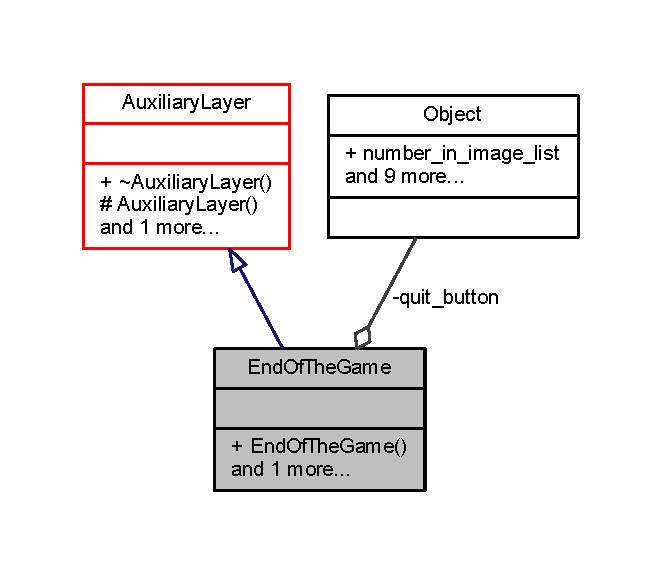
\includegraphics[width=318pt]{class_end_of_the_game__coll__graph}
\end{center}
\end{figure}
\subsection*{Public Member Functions}
\begin{DoxyCompactItemize}
\item 
\mbox{\Hypertarget{class_end_of_the_game_a27eaa843d569afd8565ed6369ea82e4f}\label{class_end_of_the_game_a27eaa843d569afd8565ed6369ea82e4f}} 
\hyperlink{class_end_of_the_game_a27eaa843d569afd8565ed6369ea82e4f}{End\+Of\+The\+Game} ()
\begin{DoxyCompactList}\small\item\em Default constructor. \end{DoxyCompactList}\item 
void \hyperlink{class_end_of_the_game_a88ac00a6aaa5193c7642d9ea2c6be688}{smth\+Happend} (\hyperlink{_events_8h_af60e00b78607064c5be6aa9397ea49c1}{Events} what\+\_\+happened)
\begin{DoxyCompactList}\small\item\em Listener of player action. \end{DoxyCompactList}\end{DoxyCompactItemize}
\subsection*{Private Attributes}
\begin{DoxyCompactItemize}
\item 
\mbox{\Hypertarget{class_end_of_the_game_af4d60352787faf883df1eec46183eee9}\label{class_end_of_the_game_af4d60352787faf883df1eec46183eee9}} 
\hyperlink{class_object}{Object} $\ast$ \hyperlink{class_end_of_the_game_af4d60352787faf883df1eec46183eee9}{quit\+\_\+button}
\begin{DoxyCompactList}\small\item\em Pointer to object contain button \char`\"{}quit\char`\"{}. \end{DoxyCompactList}\end{DoxyCompactItemize}
\subsection*{Additional Inherited Members}


\subsection{Detailed Description}
\char`\"{}\+The End\char`\"{} screen 

\begin{DoxyAuthor}{Author}
Vasily 
\end{DoxyAuthor}
\begin{DoxyVersion}{Version}
1.\+0 
\end{DoxyVersion}
\begin{DoxyDate}{Date}
June 2017
\end{DoxyDate}
Stores information needed to display \char`\"{}\+The End\char`\"{} screen 

\subsection{Member Function Documentation}
\mbox{\Hypertarget{class_end_of_the_game_a88ac00a6aaa5193c7642d9ea2c6be688}\label{class_end_of_the_game_a88ac00a6aaa5193c7642d9ea2c6be688}} 
\index{End\+Of\+The\+Game@{End\+Of\+The\+Game}!smth\+Happend@{smth\+Happend}}
\index{smth\+Happend@{smth\+Happend}!End\+Of\+The\+Game@{End\+Of\+The\+Game}}
\subsubsection{\texorpdfstring{smth\+Happend()}{smthHappend()}}
{\footnotesize\ttfamily void End\+Of\+The\+Game\+::smth\+Happend (\begin{DoxyParamCaption}\item[{\hyperlink{_events_8h_af60e00b78607064c5be6aa9397ea49c1}{Events}}]{what\+\_\+happened }\end{DoxyParamCaption})\hspace{0.3cm}{\ttfamily [virtual]}}



Listener of player action. 

Virtual method, inhereted from \hyperlink{class_layer}{Layer} class, which allow react to user action 
\begin{DoxyParams}{Parameters}
{\em what\+\_\+happened} & enum describing player action \\
\hline
\end{DoxyParams}


Implements \hyperlink{class_layer_a41318993a0f6c7ba3bc6d964f7802c10}{Layer}.



The documentation for this class was generated from the following files\+:\begin{DoxyCompactItemize}
\item 
\hyperlink{_end_of_the_game_8h}{End\+Of\+The\+Game.\+h}\item 
End\+Of\+The\+Game.\+cpp\end{DoxyCompactItemize}

\hypertarget{class_error_window}{}\section{Error\+Window Class Reference}
\label{class_error_window}\index{Error\+Window@{Error\+Window}}


\char`\"{}\+The Error\char`\"{} screen  




{\ttfamily \#include $<$Error\+Window.\+h$>$}



Collaboration diagram for Error\+Window\+:\nopagebreak
\begin{figure}[H]
\begin{center}
\leavevmode
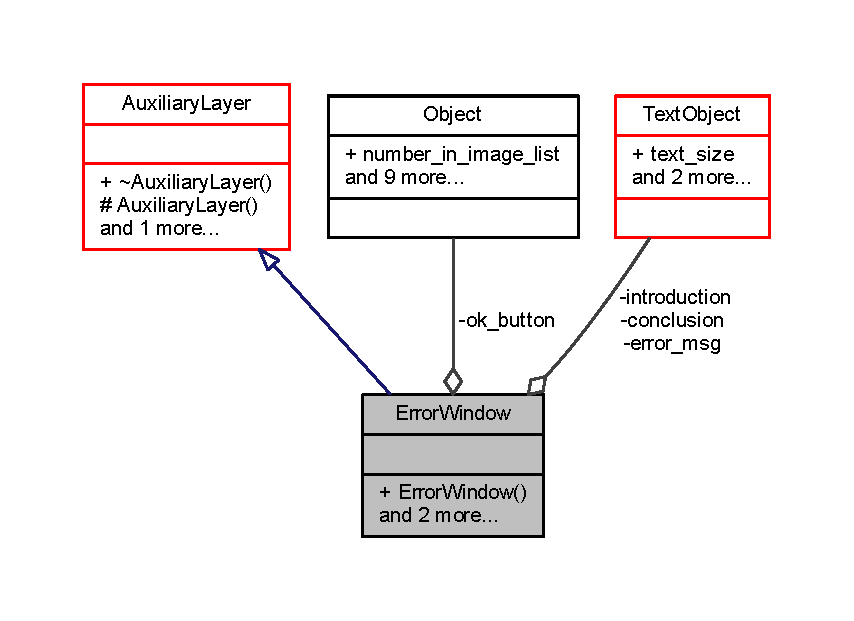
\includegraphics[width=350pt]{class_error_window__coll__graph}
\end{center}
\end{figure}
\subsection*{Public Member Functions}
\begin{DoxyCompactItemize}
\item 
\mbox{\Hypertarget{class_error_window_a6a1f634d7aab03610249b4988f374314}\label{class_error_window_a6a1f634d7aab03610249b4988f374314}} 
\hyperlink{class_error_window_a6a1f634d7aab03610249b4988f374314}{Error\+Window} ()
\begin{DoxyCompactList}\small\item\em Default constructor. \end{DoxyCompactList}\item 
void \hyperlink{class_error_window_ac5adc252881ca2932b4804a51da44d3e}{set\+Error\+Msg} (std\+::string \hyperlink{class_error_window_ad282b1abbf57a6c004b1ccfa48355f49}{error\+\_\+msg})
\begin{DoxyCompactList}\small\item\em Set error message to display. \end{DoxyCompactList}\item 
void \hyperlink{class_error_window_af9096dfdd53c4e788e62ce543f939f01}{smth\+Happend} (\hyperlink{_events_8h_af60e00b78607064c5be6aa9397ea49c1}{Events} what\+\_\+happened)
\begin{DoxyCompactList}\small\item\em Listener of player action. \end{DoxyCompactList}\end{DoxyCompactItemize}
\subsection*{Private Attributes}
\begin{DoxyCompactItemize}
\item 
\mbox{\Hypertarget{class_error_window_af19cefec0afdefc61a143fbba66a293b}\label{class_error_window_af19cefec0afdefc61a143fbba66a293b}} 
\hyperlink{class_text_object}{Text\+Object} \hyperlink{class_error_window_af19cefec0afdefc61a143fbba66a293b}{introduction}
\begin{DoxyCompactList}\small\item\em Heading of the screen. \end{DoxyCompactList}\item 
\mbox{\Hypertarget{class_error_window_ad282b1abbf57a6c004b1ccfa48355f49}\label{class_error_window_ad282b1abbf57a6c004b1ccfa48355f49}} 
\hyperlink{class_text_object}{Text\+Object} \hyperlink{class_error_window_ad282b1abbf57a6c004b1ccfa48355f49}{error\+\_\+msg}
\begin{DoxyCompactList}\small\item\em Error message. \end{DoxyCompactList}\item 
\mbox{\Hypertarget{class_error_window_a0f1580b68d4e10e07b4cd7d03a6431c4}\label{class_error_window_a0f1580b68d4e10e07b4cd7d03a6431c4}} 
\hyperlink{class_text_object}{Text\+Object} \hyperlink{class_error_window_a0f1580b68d4e10e07b4cd7d03a6431c4}{conclusion}
\begin{DoxyCompactList}\small\item\em Recommendation for user to contact developer. \end{DoxyCompactList}\item 
\mbox{\Hypertarget{class_error_window_aa155c8753f726ace716eabca851255dc}\label{class_error_window_aa155c8753f726ace716eabca851255dc}} 
\hyperlink{class_object}{Object} $\ast$ \hyperlink{class_error_window_aa155c8753f726ace716eabca851255dc}{ok\+\_\+button}
\begin{DoxyCompactList}\small\item\em Pointer to object contain button \char`\"{}\+O\+K\char`\"{}. \end{DoxyCompactList}\end{DoxyCompactItemize}
\subsection*{Additional Inherited Members}


\subsection{Detailed Description}
\char`\"{}\+The Error\char`\"{} screen 

\begin{DoxyAuthor}{Author}
Vasily 
\end{DoxyAuthor}
\begin{DoxyVersion}{Version}
1.\+0 
\end{DoxyVersion}
\begin{DoxyDate}{Date}
June 2017
\end{DoxyDate}
Stores information needed to display \char`\"{}\+The Error\char`\"{} screen 

\subsection{Member Function Documentation}
\mbox{\Hypertarget{class_error_window_ac5adc252881ca2932b4804a51da44d3e}\label{class_error_window_ac5adc252881ca2932b4804a51da44d3e}} 
\index{Error\+Window@{Error\+Window}!set\+Error\+Msg@{set\+Error\+Msg}}
\index{set\+Error\+Msg@{set\+Error\+Msg}!Error\+Window@{Error\+Window}}
\subsubsection{\texorpdfstring{set\+Error\+Msg()}{setErrorMsg()}}
{\footnotesize\ttfamily void Error\+Window\+::set\+Error\+Msg (\begin{DoxyParamCaption}\item[{std\+::string}]{error\+\_\+msg }\end{DoxyParamCaption})}



Set error message to display. 


\begin{DoxyParams}{Parameters}
{\em error\+\_\+msg} & string containing error message \\
\hline
\end{DoxyParams}
\mbox{\Hypertarget{class_error_window_af9096dfdd53c4e788e62ce543f939f01}\label{class_error_window_af9096dfdd53c4e788e62ce543f939f01}} 
\index{Error\+Window@{Error\+Window}!smth\+Happend@{smth\+Happend}}
\index{smth\+Happend@{smth\+Happend}!Error\+Window@{Error\+Window}}
\subsubsection{\texorpdfstring{smth\+Happend()}{smthHappend()}}
{\footnotesize\ttfamily void Error\+Window\+::smth\+Happend (\begin{DoxyParamCaption}\item[{\hyperlink{_events_8h_af60e00b78607064c5be6aa9397ea49c1}{Events}}]{what\+\_\+happened }\end{DoxyParamCaption})\hspace{0.3cm}{\ttfamily [virtual]}}



Listener of player action. 

Virtual method, inhereted from \hyperlink{class_layer}{Layer} class, which allow react to user action 
\begin{DoxyParams}{Parameters}
{\em what\+\_\+happened} & enum describing player action \\
\hline
\end{DoxyParams}


Implements \hyperlink{class_layer_a41318993a0f6c7ba3bc6d964f7802c10}{Layer}.



The documentation for this class was generated from the following files\+:\begin{DoxyCompactItemize}
\item 
\hyperlink{_error_window_8h}{Error\+Window.\+h}\item 
Error\+Window.\+cpp\end{DoxyCompactItemize}

\hypertarget{class_final}{}\section{Final Class Reference}
\label{class_final}\index{Final@{Final}}


Collaboration diagram for Final\+:\nopagebreak
\begin{figure}[H]
\begin{center}
\leavevmode
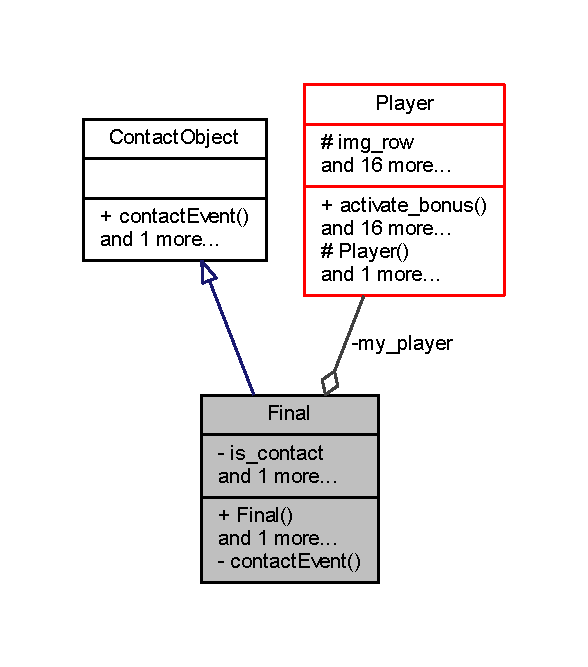
\includegraphics[width=282pt]{class_final__coll__graph}
\end{center}
\end{figure}
\subsection*{Public Member Functions}
\begin{DoxyCompactItemize}
\item 
\mbox{\Hypertarget{class_final_ad8e4afdefd9ea952bfbb7123af09c710}\label{class_final_ad8e4afdefd9ea952bfbb7123af09c710}} 
{\bfseries Final} (b2\+Body $\ast$body, bool is\+\_\+strong)
\item 
\mbox{\Hypertarget{class_final_af7a2beabd2de1cc0fcbe017f2012e41c}\label{class_final_af7a2beabd2de1cc0fcbe017f2012e41c}} 
bool {\bfseries is\+Reach} ()
\end{DoxyCompactItemize}
\subsection*{Private Member Functions}
\begin{DoxyCompactItemize}
\item 
void \hyperlink{class_final_a9ebc21296dd28e993f2ee8cbb47a3b37}{contact\+Event} (b2\+Contact $\ast$, bool)
\begin{DoxyCompactList}\small\item\em Define object reaction to the collision in box2d world. \end{DoxyCompactList}\end{DoxyCompactItemize}
\subsection*{Private Attributes}
\begin{DoxyCompactItemize}
\item 
\mbox{\Hypertarget{class_final_ac09c1e5af1c2317a59fd2bdac39aac9f}\label{class_final_ac09c1e5af1c2317a59fd2bdac39aac9f}} 
\hyperlink{class_player}{Player} $\ast$ {\bfseries my\+\_\+player}
\item 
\mbox{\Hypertarget{class_final_a637485b836c9226c062c92a34e0a679d}\label{class_final_a637485b836c9226c062c92a34e0a679d}} 
bool {\bfseries is\+\_\+contact}
\item 
\mbox{\Hypertarget{class_final_a4beb08f8f72e6339e8544ae121fb717d}\label{class_final_a4beb08f8f72e6339e8544ae121fb717d}} 
bool {\bfseries is\+\_\+strong}
\end{DoxyCompactItemize}


\subsection{Member Function Documentation}
\mbox{\Hypertarget{class_final_a9ebc21296dd28e993f2ee8cbb47a3b37}\label{class_final_a9ebc21296dd28e993f2ee8cbb47a3b37}} 
\index{Final@{Final}!contact\+Event@{contact\+Event}}
\index{contact\+Event@{contact\+Event}!Final@{Final}}
\subsubsection{\texorpdfstring{contact\+Event()}{contactEvent()}}
{\footnotesize\ttfamily void Final\+::contact\+Event (\begin{DoxyParamCaption}\item[{b2\+Contact $\ast$}]{contact,  }\item[{bool}]{is\+Begin }\end{DoxyParamCaption})\hspace{0.3cm}{\ttfamily [private]}, {\ttfamily [virtual]}}



Define object reaction to the collision in box2d world. 


\begin{DoxyParams}{Parameters}
{\em contact} & pointer to box2d b2\+Contact class \\
\hline
{\em is\+Begin} & \textquotesingle{}false\textquotesingle{} -\/ end of the collision; \textquotesingle{}true\textquotesingle{} -\/ start of the collision \\
\hline
\end{DoxyParams}


Implements \hyperlink{class_contact_object_a53d2dfc1d9c2821e9c62e80ce62a6435}{Contact\+Object}.



The documentation for this class was generated from the following files\+:\begin{DoxyCompactItemize}
\item 
Final.\+h\item 
Final.\+cpp\end{DoxyCompactItemize}

\hypertarget{class_game_over}{}\section{Game\+Over Class Reference}
\label{class_game_over}\index{Game\+Over@{Game\+Over}}


\char`\"{}\+Game Over\char`\"{} screen  




{\ttfamily \#include $<$Game\+Over.\+h$>$}



Collaboration diagram for Game\+Over\+:
\nopagebreak
\begin{figure}[H]
\begin{center}
\leavevmode
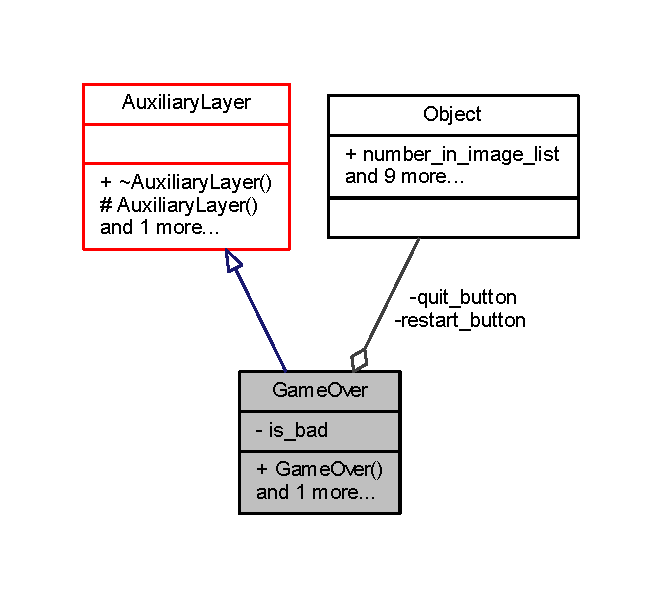
\includegraphics[width=318pt]{class_game_over__coll__graph}
\end{center}
\end{figure}
\subsection*{Public Member Functions}
\begin{DoxyCompactItemize}
\item 
\hyperlink{class_game_over_a3eb13fd94a63ff6dace1e1265b0c535d}{Game\+Over} (bool \hyperlink{class_game_over_a4a7103cf4db129cad83b0c001c32d116}{is\+\_\+bad})
\item 
void \hyperlink{class_game_over_a919e7ac37c476bf288f732f9a8106016}{smth\+Happend} (\hyperlink{_events_8h_af60e00b78607064c5be6aa9397ea49c1}{Events} what\+\_\+happened)
\begin{DoxyCompactList}\small\item\em Listener of player action. \end{DoxyCompactList}\end{DoxyCompactItemize}
\subsection*{Private Attributes}
\begin{DoxyCompactItemize}
\item 
\mbox{\Hypertarget{class_game_over_a5d017200c062c83022d9efe2c29e0633}\label{class_game_over_a5d017200c062c83022d9efe2c29e0633}} 
\hyperlink{class_object}{Object} $\ast$ \hyperlink{class_game_over_a5d017200c062c83022d9efe2c29e0633}{restart\+\_\+button}
\begin{DoxyCompactList}\small\item\em Pointer to object contain button \char`\"{}\+Restart\char`\"{}. \end{DoxyCompactList}\item 
\mbox{\Hypertarget{class_game_over_a60a67578fd38fa4f4b464f69edc7ef9b}\label{class_game_over_a60a67578fd38fa4f4b464f69edc7ef9b}} 
\hyperlink{class_object}{Object} $\ast$ \hyperlink{class_game_over_a60a67578fd38fa4f4b464f69edc7ef9b}{quit\+\_\+button}
\begin{DoxyCompactList}\small\item\em Pointer to object contain button \char`\"{}\+Quit\char`\"{}. \end{DoxyCompactList}\item 
bool \hyperlink{class_game_over_a4a7103cf4db129cad83b0c001c32d116}{is\+\_\+bad}
\begin{DoxyCompactList}\small\item\em Define type of the screen. \end{DoxyCompactList}\end{DoxyCompactItemize}
\subsection*{Additional Inherited Members}


\subsection{Detailed Description}
\char`\"{}\+Game Over\char`\"{} screen 

\begin{DoxyAuthor}{Author}
Vasily 
\end{DoxyAuthor}
\begin{DoxyVersion}{Version}
1.\+0 
\end{DoxyVersion}
\begin{DoxyDate}{Date}
June 2017
\end{DoxyDate}
Stores information needed to display \char`\"{}\+Game Over\char`\"{} or \char`\"{}\+You win\char`\"{} screen 

\subsection{Constructor \& Destructor Documentation}
\mbox{\Hypertarget{class_game_over_a3eb13fd94a63ff6dace1e1265b0c535d}\label{class_game_over_a3eb13fd94a63ff6dace1e1265b0c535d}} 
\index{Game\+Over@{Game\+Over}!Game\+Over@{Game\+Over}}
\index{Game\+Over@{Game\+Over}!Game\+Over@{Game\+Over}}
\subsubsection{\texorpdfstring{Game\+Over()}{GameOver()}}
{\footnotesize\ttfamily Game\+Over\+::\+Game\+Over (\begin{DoxyParamCaption}\item[{bool}]{is\+\_\+bad }\end{DoxyParamCaption})}


\begin{DoxyParams}{Parameters}
{\em is\+\_\+bad} & set the type of the screen (see is\+\_\+bad private flag) \\
\hline
\end{DoxyParams}


\subsection{Member Function Documentation}
\mbox{\Hypertarget{class_game_over_a919e7ac37c476bf288f732f9a8106016}\label{class_game_over_a919e7ac37c476bf288f732f9a8106016}} 
\index{Game\+Over@{Game\+Over}!smth\+Happend@{smth\+Happend}}
\index{smth\+Happend@{smth\+Happend}!Game\+Over@{Game\+Over}}
\subsubsection{\texorpdfstring{smth\+Happend()}{smthHappend()}}
{\footnotesize\ttfamily void Game\+Over\+::smth\+Happend (\begin{DoxyParamCaption}\item[{\hyperlink{_events_8h_af60e00b78607064c5be6aa9397ea49c1}{Events}}]{what\+\_\+happened }\end{DoxyParamCaption})\hspace{0.3cm}{\ttfamily [virtual]}}



Listener of player action. 

Virtual method, inhereted from \hyperlink{class_layer}{Layer} class, which allow react to user action 
\begin{DoxyParams}{Parameters}
{\em what\+\_\+happened} & enum describing player action \\
\hline
\end{DoxyParams}


Implements \hyperlink{class_layer_a41318993a0f6c7ba3bc6d964f7802c10}{Layer}.



\subsection{Member Data Documentation}
\mbox{\Hypertarget{class_game_over_a4a7103cf4db129cad83b0c001c32d116}\label{class_game_over_a4a7103cf4db129cad83b0c001c32d116}} 
\index{Game\+Over@{Game\+Over}!is\+\_\+bad@{is\+\_\+bad}}
\index{is\+\_\+bad@{is\+\_\+bad}!Game\+Over@{Game\+Over}}
\subsubsection{\texorpdfstring{is\+\_\+bad}{is\_bad}}
{\footnotesize\ttfamily bool Game\+Over\+::is\+\_\+bad\hspace{0.3cm}{\ttfamily [private]}}



Define type of the screen. 


\begin{DoxyParams}{Parameters}
{\em false} & \char`\"{}\+You win\char`\"{} screen \\
\hline
{\em true} & \char`\"{}\+Game over\char`\"{} screen \\
\hline
\end{DoxyParams}


The documentation for this class was generated from the following files\+:\begin{DoxyCompactItemize}
\item 
\hyperlink{_game_over_8h}{Game\+Over.\+h}\item 
Game\+Over.\+cpp\end{DoxyCompactItemize}

\hypertarget{class_layer}{}\section{Layer Class Reference}
\label{class_layer}\index{Layer@{Layer}}


Determines a certain state of the model.  




{\ttfamily \#include $<$Layer.\+h$>$}



Collaboration diagram for Layer\+:\nopagebreak
\begin{figure}[H]
\begin{center}
\leavevmode
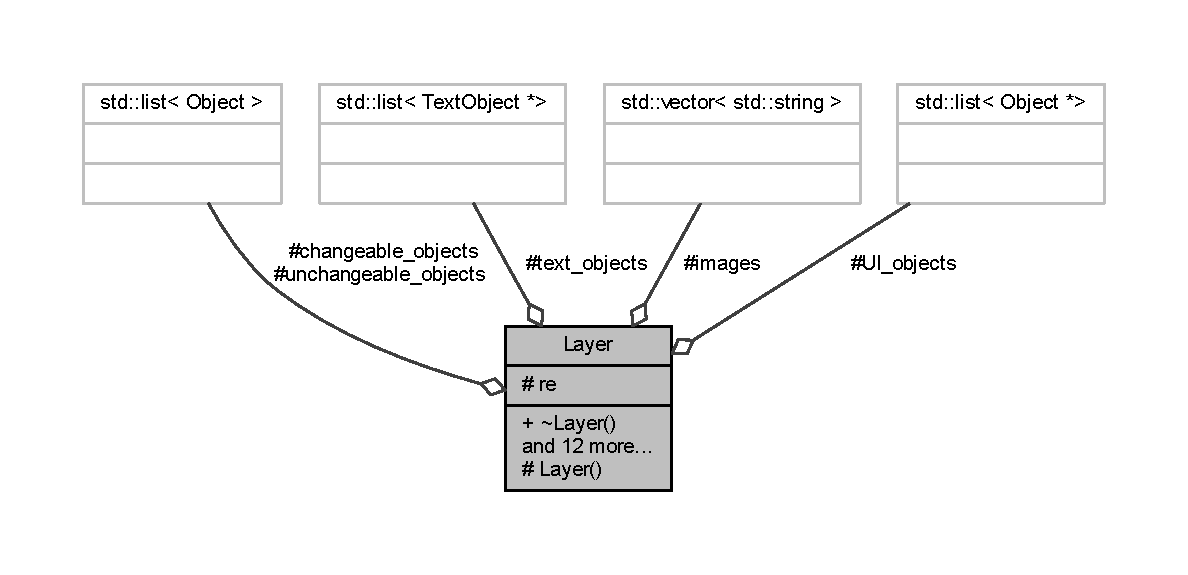
\includegraphics[width=350pt]{class_layer__coll__graph}
\end{center}
\end{figure}
\subsection*{Public Member Functions}
\begin{DoxyCompactItemize}
\item 
std\+::list$<$ \hyperlink{class_object}{Object} $>$ \hyperlink{class_layer_a88251ea7cc836a16dbca1e134c5a5ee5}{get\+Unchangeable\+Objects} ()
\item 
std\+::list$<$ \hyperlink{class_object}{Object} $>$ \hyperlink{class_layer_af1303bfbd28803f32708729f54ca13ec}{get\+Changeable\+Objects} ()
\item 
std\+::list$<$ \hyperlink{class_object}{Object} $\ast$ $>$ \hyperlink{class_layer_a2aebff84a5f25f25d56d3886c8c3a4b1}{get\+U\+I\+Objects} ()
\item 
std\+::list$<$ \hyperlink{class_text_object}{Text\+Object} $\ast$ $>$ \hyperlink{class_layer_abd1a2a8242a5d43b389e896a3d3de800}{get\+Text\+Objects} ()
\item 
virtual void \hyperlink{class_layer_a62b75693308f561bd8454a32dab9e10f}{get\+Layer\+Size} (double $\ast$width, double $\ast$height)
\begin{DoxyCompactList}\small\item\em provides opportunity to get layer width and height \end{DoxyCompactList}\item 
virtual void \hyperlink{class_layer_af2778374314bfe517007c0b0ac3fc896}{get\+Layer\+Center} (double $\ast$x, double $\ast$y)
\begin{DoxyCompactList}\small\item\em provides opportunity to get layer center \end{DoxyCompactList}\item 
virtual bool \hyperlink{class_layer_a952ad194d28fe6999b85bd3d9d28ee31}{is\+Double\+View} ()
\begin{DoxyCompactList}\small\item\em return the number of view entity on the level \end{DoxyCompactList}\item 
virtual void \hyperlink{class_layer_a41318993a0f6c7ba3bc6d964f7802c10}{smth\+Happend} (\hyperlink{_events_8h_af60e00b78607064c5be6aa9397ea49c1}{Events} what\+\_\+happened)=0
\begin{DoxyCompactList}\small\item\em Listener of player action. \end{DoxyCompactList}\item 
\mbox{\Hypertarget{class_layer_a9e197da9a85a455af77c83301ebb4d1d}\label{class_layer_a9e197da9a85a455af77c83301ebb4d1d}} 
virtual void \hyperlink{class_layer_a9e197da9a85a455af77c83301ebb4d1d}{repause} ()
\begin{DoxyCompactList}\small\item\em informs that level again active \end{DoxyCompactList}\item 
\mbox{\Hypertarget{class_layer_a4243d1a4b059eb7433cbfe7cdfc2c191}\label{class_layer_a4243d1a4b059eb7433cbfe7cdfc2c191}} 
virtual void \hyperlink{class_layer_a4243d1a4b059eb7433cbfe7cdfc2c191}{update} ()
\begin{DoxyCompactList}\small\item\em update layer state \end{DoxyCompactList}\item 
virtual std\+::vector$<$ std\+::string $>$ \& \hyperlink{class_layer_a9acbfda611b85762f4a39ece4ea4df33}{get\+Images\+List} ()
\item 
virtual \hyperlink{_events_8h_a51620cf702f1b8fdf47cd0a5cfa0ba4f}{Return\+Events} $\ast$ \hyperlink{class_layer_ac57343394c8dba2a180a7762cd3a20b6}{get\+Ret\+Event} ()
\end{DoxyCompactItemize}
\subsection*{Protected Attributes}
\begin{DoxyCompactItemize}
\item 
\mbox{\Hypertarget{class_layer_ada06fdf26fe10efb2bb66ada8d10d3e0}\label{class_layer_ada06fdf26fe10efb2bb66ada8d10d3e0}} 
std\+::list$<$ \hyperlink{class_object}{Object} $>$ \hyperlink{class_layer_ada06fdf26fe10efb2bb66ada8d10d3e0}{unchangeable\+\_\+objects}
\begin{DoxyCompactList}\small\item\em list of an layers objects which can\textquotesingle{}t change during simulation process \end{DoxyCompactList}\item 
\mbox{\Hypertarget{class_layer_a6e160468d3c84bba8324a11b05be6b6e}\label{class_layer_a6e160468d3c84bba8324a11b05be6b6e}} 
std\+::list$<$ \hyperlink{class_object}{Object} $>$ \hyperlink{class_layer_a6e160468d3c84bba8324a11b05be6b6e}{changeable\+\_\+objects}
\begin{DoxyCompactList}\small\item\em list of an layers objects which can change during simulation process \end{DoxyCompactList}\item 
\mbox{\Hypertarget{class_layer_a98666cc5fd94f591c3e9ffccc02ee45c}\label{class_layer_a98666cc5fd94f591c3e9ffccc02ee45c}} 
std\+::list$<$ \hyperlink{class_object}{Object} $\ast$ $>$ \hyperlink{class_layer_a98666cc5fd94f591c3e9ffccc02ee45c}{U\+I\+\_\+objects}
\begin{DoxyCompactList}\small\item\em list of an layers objects which represent layer UI \end{DoxyCompactList}\item 
\mbox{\Hypertarget{class_layer_a46c6bac93a96f1afc853aca03a42351a}\label{class_layer_a46c6bac93a96f1afc853aca03a42351a}} 
std\+::list$<$ \hyperlink{class_text_object}{Text\+Object} $\ast$ $>$ \hyperlink{class_layer_a46c6bac93a96f1afc853aca03a42351a}{text\+\_\+objects}
\begin{DoxyCompactList}\small\item\em list of an layers text objects \end{DoxyCompactList}\item 
\mbox{\Hypertarget{class_layer_a0bfe2f79d24415f8619a4a7491bf1fd8}\label{class_layer_a0bfe2f79d24415f8619a4a7491bf1fd8}} 
std\+::vector$<$ std\+::string $>$ \hyperlink{class_layer_a0bfe2f79d24415f8619a4a7491bf1fd8}{images}
\begin{DoxyCompactList}\small\item\em list of string names for all images dispalyes at this layer \end{DoxyCompactList}\item 
\mbox{\Hypertarget{class_layer_a157765c60d80f37a81c5f317da6495fe}\label{class_layer_a157765c60d80f37a81c5f317da6495fe}} 
\hyperlink{_events_8h_a51620cf702f1b8fdf47cd0a5cfa0ba4f}{Return\+Events} \hyperlink{class_layer_a157765c60d80f37a81c5f317da6495fe}{re}
\begin{DoxyCompactList}\small\item\em last event that happens at this layer \end{DoxyCompactList}\end{DoxyCompactItemize}


\subsection{Detailed Description}
Determines a certain state of the model. 

\begin{DoxyAuthor}{Author}
Vasily 
\end{DoxyAuthor}
\begin{DoxyVersion}{Version}
1.\+0 
\end{DoxyVersion}
\begin{DoxyDate}{Date}
June 2017
\end{DoxyDate}
Class-\/layer with which works \hyperlink{class_model}{Model} class 

\subsection{Member Function Documentation}
\mbox{\Hypertarget{class_layer_af1303bfbd28803f32708729f54ca13ec}\label{class_layer_af1303bfbd28803f32708729f54ca13ec}} 
\index{Layer@{Layer}!get\+Changeable\+Objects@{get\+Changeable\+Objects}}
\index{get\+Changeable\+Objects@{get\+Changeable\+Objects}!Layer@{Layer}}
\subsubsection{\texorpdfstring{get\+Changeable\+Objects()}{getChangeableObjects()}}
{\footnotesize\ttfamily std\+::list$<$ \hyperlink{class_object}{Object} $>$ Layer\+::get\+Changeable\+Objects (\begin{DoxyParamCaption}{ }\end{DoxyParamCaption})}

\begin{DoxyReturn}{Returns}
list of an layers objects which can change during simulation process 
\end{DoxyReturn}
\mbox{\Hypertarget{class_layer_a9acbfda611b85762f4a39ece4ea4df33}\label{class_layer_a9acbfda611b85762f4a39ece4ea4df33}} 
\index{Layer@{Layer}!get\+Images\+List@{get\+Images\+List}}
\index{get\+Images\+List@{get\+Images\+List}!Layer@{Layer}}
\subsubsection{\texorpdfstring{get\+Images\+List()}{getImagesList()}}
{\footnotesize\ttfamily std\+::vector$<$ std\+::string $>$ \& Layer\+::get\+Images\+List (\begin{DoxyParamCaption}{ }\end{DoxyParamCaption})\hspace{0.3cm}{\ttfamily [virtual]}}

\begin{DoxyReturn}{Returns}
list of string names for all images dispalyes at this layer 
\end{DoxyReturn}
\mbox{\Hypertarget{class_layer_af2778374314bfe517007c0b0ac3fc896}\label{class_layer_af2778374314bfe517007c0b0ac3fc896}} 
\index{Layer@{Layer}!get\+Layer\+Center@{get\+Layer\+Center}}
\index{get\+Layer\+Center@{get\+Layer\+Center}!Layer@{Layer}}
\subsubsection{\texorpdfstring{get\+Layer\+Center()}{getLayerCenter()}}
{\footnotesize\ttfamily void Layer\+::get\+Layer\+Center (\begin{DoxyParamCaption}\item[{double $\ast$}]{x,  }\item[{double $\ast$}]{y }\end{DoxyParamCaption})\hspace{0.3cm}{\ttfamily [virtual]}}



provides opportunity to get layer center 


\begin{DoxyParams}{Parameters}
{\em x} & pointer to the variable where x coordinate will be written \\
\hline
{\em y} & pointer to the variable where y coordinate will be written \\
\hline
\end{DoxyParams}


Reimplemented in \hyperlink{class_level_a4c49b93b4c3060fd650890790fc677e9}{Level}.

\mbox{\Hypertarget{class_layer_a62b75693308f561bd8454a32dab9e10f}\label{class_layer_a62b75693308f561bd8454a32dab9e10f}} 
\index{Layer@{Layer}!get\+Layer\+Size@{get\+Layer\+Size}}
\index{get\+Layer\+Size@{get\+Layer\+Size}!Layer@{Layer}}
\subsubsection{\texorpdfstring{get\+Layer\+Size()}{getLayerSize()}}
{\footnotesize\ttfamily void Layer\+::get\+Layer\+Size (\begin{DoxyParamCaption}\item[{double $\ast$}]{width,  }\item[{double $\ast$}]{height }\end{DoxyParamCaption})\hspace{0.3cm}{\ttfamily [virtual]}}



provides opportunity to get layer width and height 


\begin{DoxyParams}{Parameters}
{\em width} & pointer to the variable where width will be written \\
\hline
{\em height} & pointer to the variable where height will be written \\
\hline
\end{DoxyParams}


Reimplemented in \hyperlink{class_level_a7909f2ebe4d0f676adf9c84db2c1abc8}{Level}.

\mbox{\Hypertarget{class_layer_ac57343394c8dba2a180a7762cd3a20b6}\label{class_layer_ac57343394c8dba2a180a7762cd3a20b6}} 
\index{Layer@{Layer}!get\+Ret\+Event@{get\+Ret\+Event}}
\index{get\+Ret\+Event@{get\+Ret\+Event}!Layer@{Layer}}
\subsubsection{\texorpdfstring{get\+Ret\+Event()}{getRetEvent()}}
{\footnotesize\ttfamily \hyperlink{_events_8h_a51620cf702f1b8fdf47cd0a5cfa0ba4f}{Return\+Events} $\ast$ Layer\+::get\+Ret\+Event (\begin{DoxyParamCaption}{ }\end{DoxyParamCaption})\hspace{0.3cm}{\ttfamily [virtual]}}

\begin{DoxyReturn}{Returns}
pointer to the last event that happens at this layer 
\end{DoxyReturn}
\mbox{\Hypertarget{class_layer_abd1a2a8242a5d43b389e896a3d3de800}\label{class_layer_abd1a2a8242a5d43b389e896a3d3de800}} 
\index{Layer@{Layer}!get\+Text\+Objects@{get\+Text\+Objects}}
\index{get\+Text\+Objects@{get\+Text\+Objects}!Layer@{Layer}}
\subsubsection{\texorpdfstring{get\+Text\+Objects()}{getTextObjects()}}
{\footnotesize\ttfamily std\+::list$<$ \hyperlink{class_text_object}{Text\+Object} $\ast$ $>$ Layer\+::get\+Text\+Objects (\begin{DoxyParamCaption}{ }\end{DoxyParamCaption})}

\begin{DoxyReturn}{Returns}
list of an layers text objects 
\end{DoxyReturn}
\mbox{\Hypertarget{class_layer_a2aebff84a5f25f25d56d3886c8c3a4b1}\label{class_layer_a2aebff84a5f25f25d56d3886c8c3a4b1}} 
\index{Layer@{Layer}!get\+U\+I\+Objects@{get\+U\+I\+Objects}}
\index{get\+U\+I\+Objects@{get\+U\+I\+Objects}!Layer@{Layer}}
\subsubsection{\texorpdfstring{get\+U\+I\+Objects()}{getUIObjects()}}
{\footnotesize\ttfamily std\+::list$<$ \hyperlink{class_object}{Object} $\ast$ $>$ Layer\+::get\+U\+I\+Objects (\begin{DoxyParamCaption}{ }\end{DoxyParamCaption})}

\begin{DoxyReturn}{Returns}
list of an layers objects which represent layer UI 
\end{DoxyReturn}
\mbox{\Hypertarget{class_layer_a88251ea7cc836a16dbca1e134c5a5ee5}\label{class_layer_a88251ea7cc836a16dbca1e134c5a5ee5}} 
\index{Layer@{Layer}!get\+Unchangeable\+Objects@{get\+Unchangeable\+Objects}}
\index{get\+Unchangeable\+Objects@{get\+Unchangeable\+Objects}!Layer@{Layer}}
\subsubsection{\texorpdfstring{get\+Unchangeable\+Objects()}{getUnchangeableObjects()}}
{\footnotesize\ttfamily std\+::list$<$ \hyperlink{class_object}{Object} $>$ Layer\+::get\+Unchangeable\+Objects (\begin{DoxyParamCaption}{ }\end{DoxyParamCaption})}

\begin{DoxyReturn}{Returns}
list of an layers objects which can\textquotesingle{}t change during simulation process 
\end{DoxyReturn}
\mbox{\Hypertarget{class_layer_a952ad194d28fe6999b85bd3d9d28ee31}\label{class_layer_a952ad194d28fe6999b85bd3d9d28ee31}} 
\index{Layer@{Layer}!is\+Double\+View@{is\+Double\+View}}
\index{is\+Double\+View@{is\+Double\+View}!Layer@{Layer}}
\subsubsection{\texorpdfstring{is\+Double\+View()}{isDoubleView()}}
{\footnotesize\ttfamily bool Layer\+::is\+Double\+View (\begin{DoxyParamCaption}{ }\end{DoxyParamCaption})\hspace{0.3cm}{\ttfamily [virtual]}}



return the number of view entity on the level 

\begin{DoxyReturn}{Returns}
\textquotesingle{}true\textquotesingle{} -\/ two entities; \textquotesingle{}false\textquotesingle{} -\/ one entity 
\end{DoxyReturn}


Reimplemented in \hyperlink{class_level_ae3584a92caee4cf544abd2c4f946cb18}{Level}.

\mbox{\Hypertarget{class_layer_a41318993a0f6c7ba3bc6d964f7802c10}\label{class_layer_a41318993a0f6c7ba3bc6d964f7802c10}} 
\index{Layer@{Layer}!smth\+Happend@{smth\+Happend}}
\index{smth\+Happend@{smth\+Happend}!Layer@{Layer}}
\subsubsection{\texorpdfstring{smth\+Happend()}{smthHappend()}}
{\footnotesize\ttfamily virtual void Layer\+::smth\+Happend (\begin{DoxyParamCaption}\item[{\hyperlink{_events_8h_af60e00b78607064c5be6aa9397ea49c1}{Events}}]{what\+\_\+happened }\end{DoxyParamCaption})\hspace{0.3cm}{\ttfamily [pure virtual]}}



Listener of player action. 

Allow react to user action 
\begin{DoxyParams}{Parameters}
{\em what\+\_\+happened} & enum describing player action \\
\hline
\end{DoxyParams}


Implemented in \hyperlink{class_level_a4e898cb21d15947077dbedfb979c63be}{Level}, \hyperlink{class_main_menu_aa4272e1cb2c70c23c869d301f2dd2110}{Main\+Menu}, \hyperlink{class_error_window_af9096dfdd53c4e788e62ce543f939f01}{Error\+Window}, \hyperlink{class_game_over_a919e7ac37c476bf288f732f9a8106016}{Game\+Over}, \hyperlink{class_local_menu_ad6db1f0ae5757a4e25269d40f6e369af}{Local\+Menu}, and \hyperlink{class_end_of_the_game_a88ac00a6aaa5193c7642d9ea2c6be688}{End\+Of\+The\+Game}.



The documentation for this class was generated from the following files\+:\begin{DoxyCompactItemize}
\item 
\hyperlink{_layer_8h}{Layer.\+h}\item 
Layer.\+cpp\end{DoxyCompactItemize}

\hypertarget{class_level}{}\section{Level Class Reference}
\label{class_level}\index{Level@{Level}}


Contains all information about game level.  




{\ttfamily \#include $<$Level.\+h$>$}



Collaboration diagram for Level\+:
\nopagebreak
\begin{figure}[H]
\begin{center}
\leavevmode
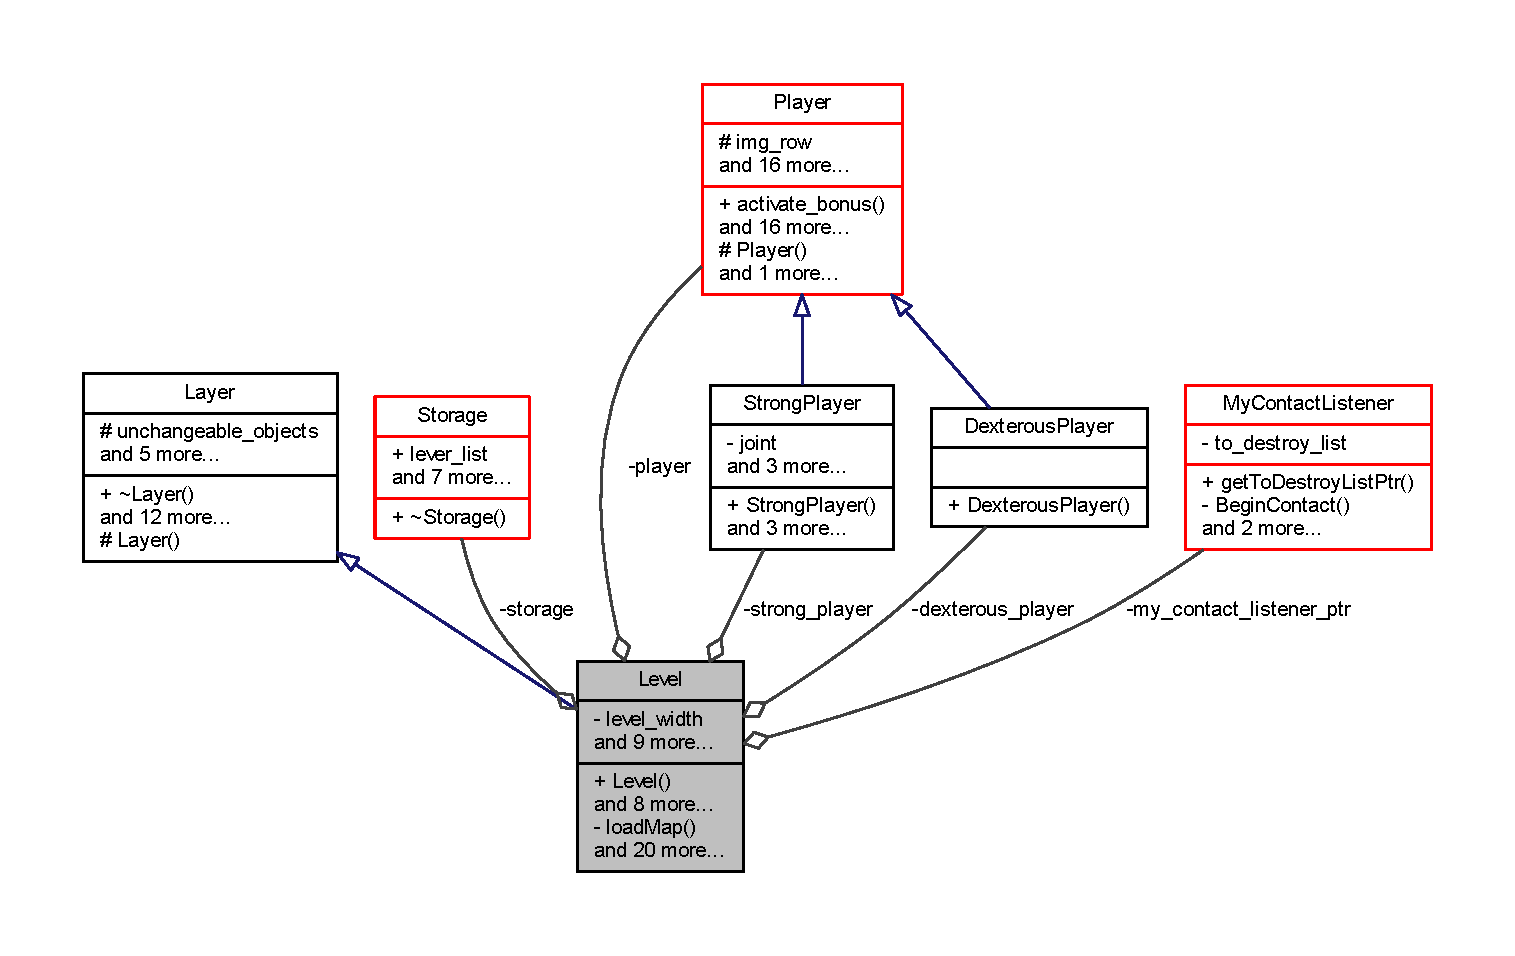
\includegraphics[width=350pt]{class_level__coll__graph}
\end{center}
\end{figure}
\subsection*{Public Member Functions}
\begin{DoxyCompactItemize}
\item 
\hyperlink{class_level_ae66cbb137b426e4dd1c9f0566ca04aa1}{Level} (std\+::string \hyperlink{class_level_a08f8815ed6a37bb8b1a2c045946cdd68}{prefix}, std\+::string filename)
\begin{DoxyCompactList}\small\item\em Defined constructor for this class. \end{DoxyCompactList}\item 
\mbox{\Hypertarget{class_level_a4e898cb21d15947077dbedfb979c63be}\label{class_level_a4e898cb21d15947077dbedfb979c63be}} 
void \hyperlink{class_level_a4e898cb21d15947077dbedfb979c63be}{smth\+Happend} (\hyperlink{_events_8h_af60e00b78607064c5be6aa9397ea49c1}{Events} what\+\_\+happened)
\begin{DoxyCompactList}\small\item\em inhereted from \hyperlink{class_layer}{Layer} class \end{DoxyCompactList}\item 
\mbox{\Hypertarget{class_level_ae3584a92caee4cf544abd2c4f946cb18}\label{class_level_ae3584a92caee4cf544abd2c4f946cb18}} 
bool \hyperlink{class_level_ae3584a92caee4cf544abd2c4f946cb18}{is\+Double\+View} ()
\begin{DoxyCompactList}\small\item\em inhereted from \hyperlink{class_layer}{Layer} class \end{DoxyCompactList}\item 
\mbox{\Hypertarget{class_level_a7909f2ebe4d0f676adf9c84db2c1abc8}\label{class_level_a7909f2ebe4d0f676adf9c84db2c1abc8}} 
void \hyperlink{class_level_a7909f2ebe4d0f676adf9c84db2c1abc8}{get\+Layer\+Size} (double $\ast$width, double $\ast$height)
\begin{DoxyCompactList}\small\item\em inhereted from \hyperlink{class_layer}{Layer} class \end{DoxyCompactList}\item 
\mbox{\Hypertarget{class_level_a4c49b93b4c3060fd650890790fc677e9}\label{class_level_a4c49b93b4c3060fd650890790fc677e9}} 
void \hyperlink{class_level_a4c49b93b4c3060fd650890790fc677e9}{get\+Layer\+Center} (double $\ast$x, double $\ast$y)
\begin{DoxyCompactList}\small\item\em inhereted from \hyperlink{class_layer}{Layer} class \end{DoxyCompactList}\item 
\mbox{\Hypertarget{class_level_a62e412eaad753d2baa2f94239cb80e41}\label{class_level_a62e412eaad753d2baa2f94239cb80e41}} 
void \hyperlink{class_level_a62e412eaad753d2baa2f94239cb80e41}{update} ()
\begin{DoxyCompactList}\small\item\em inhereted from \hyperlink{class_layer}{Layer} class \end{DoxyCompactList}\item 
\mbox{\Hypertarget{class_level_ab0ac8520d565a0ff6ae912baff7f1895}\label{class_level_ab0ac8520d565a0ff6ae912baff7f1895}} 
void \hyperlink{class_level_ab0ac8520d565a0ff6ae912baff7f1895}{repause} ()
\begin{DoxyCompactList}\small\item\em inhereted from \hyperlink{class_layer}{Layer} class \end{DoxyCompactList}\end{DoxyCompactItemize}
\subsection*{Private Member Functions}
\begin{DoxyCompactItemize}
\item 
void \hyperlink{class_level_ac95aee215b31865a7f010d077e9e59b8}{load\+Map} (tinyxml2\+::\+X\+M\+L\+Element $\ast$map)
\begin{DoxyCompactList}\small\item\em internal function which parse tmx file and load information about level tiledmap \end{DoxyCompactList}\item 
void \hyperlink{class_level_a366a0ac7ecbca8e3fa56d8e271d155a9}{load\+Objects} (tinyxml2\+::\+X\+M\+L\+Element $\ast$map)
\begin{DoxyCompactList}\small\item\em internal function which parse tmx file and load information about object groups \end{DoxyCompactList}\item 
void \hyperlink{class_level_a69835ba3b93667d000f1bd7feece7217}{load\+Object} (tinyxml2\+::\+X\+M\+L\+Element $\ast$objectgroup, \hyperlink{_level_8h_acf0ce63e34327e5bc336f9fe3d2d47a2}{Body\+Type} b\+\_\+type)
\begin{DoxyCompactList}\small\item\em internal function which parse tmx file and load information about object \end{DoxyCompactList}\item 
void \hyperlink{class_level_a2d4fd0491266cd6635edeb1f9b24d373}{parse\+Platform} (tinyxml2\+::\+X\+M\+L\+Element $\ast$object, tinyxml2\+::\+X\+M\+L\+Element $\ast$objectgroup, b2\+Body $\ast$body)
\begin{DoxyCompactList}\small\item\em internal function which fill up information about platform \& create it \end{DoxyCompactList}\item 
void \hyperlink{class_level_afe367884e3e0e7e1ca1870566eababd8}{parse\+Sensor} (tinyxml2\+::\+X\+M\+L\+Element $\ast$object, b2\+Body $\ast$body, std\+::vector$<$ \hyperlink{_manual_switch_obj_8h_a8bb1ef53467e4f61410d12822d922498}{Action} $>$ stages)
\begin{DoxyCompactList}\small\item\em internal function which fill up information about sensor \& create it \end{DoxyCompactList}\item 
void \hyperlink{class_level_a0230969dca0cd75ab48e212c3ec559ce}{parse\+Timer} (tinyxml2\+::\+X\+M\+L\+Element $\ast$object, std\+::vector$<$ \hyperlink{_manual_switch_obj_8h_a8bb1ef53467e4f61410d12822d922498}{Action} $>$ stages)
\begin{DoxyCompactList}\small\item\em internal function which fill up information about timer \& create it \end{DoxyCompactList}\item 
void \hyperlink{class_level_aa1921baab6b1d686f68d81efd235ebc4}{parse\+Bridge} (tinyxml2\+::\+X\+M\+L\+Element $\ast$object, b2\+Body $\ast$body, b2\+Body\+Def $\ast$body\+\_\+def, \hyperlink{class_object}{Object} $\ast$tmp\+\_\+obj)
\begin{DoxyCompactList}\small\item\em internal function which fill up information about bridge \& create it \end{DoxyCompactList}\item 
void \hyperlink{class_level_a4e4b69194e33200fff8f9b0282e10559}{parse\+Danger\+Object} (tinyxml2\+::\+X\+M\+L\+Element $\ast$object, b2\+Body $\ast$body, \hyperlink{class_object}{Object} $\ast$tmp\+\_\+obj, tinyxml2\+::\+X\+M\+L\+Element $\ast$objectgroup)
\begin{DoxyCompactList}\small\item\em internal function which fill up information about danger object \& create it \end{DoxyCompactList}\item 
b2\+Body $\ast$ \hyperlink{class_level_a87d0a007fafb7f51a1410f6f7114b699}{create\+Border\+Sensor} (b2\+Body $\ast$body, \hyperlink{class_object}{Object} $\ast$tmp\+\_\+obj, \hyperlink{_level_8h_aa8656d997df416abfebfcf4b3041f01c}{Sides} sides)
\begin{DoxyCompactList}\small\item\em internal function which fill up information about special player sensor \& create it \end{DoxyCompactList}\item 
\mbox{\Hypertarget{class_level_a9977ee08d7036b23eb0467a6d8d2e176}\label{class_level_a9977ee08d7036b23eb0467a6d8d2e176}} 
void \hyperlink{class_level_a9977ee08d7036b23eb0467a6d8d2e176}{add\+U\+I\+To\+Level} ()
\begin{DoxyCompactList}\small\item\em internal function which fill up information about level UI \end{DoxyCompactList}\item 
std\+::vector$<$ \hyperlink{_manual_switch_obj_8h_a8bb1ef53467e4f61410d12822d922498}{Action} $>$ \hyperlink{class_level_ab61118c640a3426f77d88990a4ddc697}{sensor\+Stages\+Parser} (std\+::vector$<$ std\+::string $>$ stages)
\begin{DoxyCompactList}\small\item\em internal function which transfer string information from from xml file to Action enum commands \end{DoxyCompactList}\item 
tinyxml2\+::\+X\+M\+L\+Element $\ast$ \hyperlink{class_level_a214fb496aebd1994f8aae99bc5f6eb24}{find\+Among\+Siblings} (tinyxml2\+::\+X\+M\+L\+Element $\ast$element, std\+::string name)
\begin{DoxyCompactList}\small\item\em internal function which find an element in X\+M\+L-\/file among similar \end{DoxyCompactList}\item 
{\footnotesize template$<$typename T $>$ }\\auto \hyperlink{class_level_ada3610b170f131ef23847ca47743e0f7}{check\+Element\+Existence} (const T smf\+\_\+to\+\_\+check, std\+::string error\+\_\+msg)
\begin{DoxyCompactList}\small\item\em subsidiary function which check existense of the element and throw exception if it isn\textquotesingle{}t \end{DoxyCompactList}\item 
std\+::string \hyperlink{class_level_a1965bb306d89207706d1e9ac315ffb43}{file\+Exists\+Test} (const std\+::string \&name)
\begin{DoxyCompactList}\small\item\em subsidiary function which check existense of the file and throw exception if it isn\textquotesingle{}t \end{DoxyCompactList}\item 
std\+::vector$<$ std\+::string $>$ \hyperlink{class_level_a6aecafb8e2e9a33178c9d18d100d7261}{string\+Delimiter} (std\+::string init\+\_\+str)
\begin{DoxyCompactList}\small\item\em subsidiary function which devides string using \textquotesingle{}space\textquotesingle{} as delimiters \end{DoxyCompactList}\item 
std\+::vector$<$ std\+::pair$<$ double, double $>$ $>$ \hyperlink{class_level_ac8bdc4273913a8f0bf8523c6fe20450a}{build\+Trajectory} (tinyxml2\+::\+X\+M\+L\+Element $\ast$objectgroup, std\+::string trajectory\+\_\+name, bool $\ast$is\+\_\+rounded)
\begin{DoxyCompactList}\small\item\em subsidiary function fill up vector with two-\/coordinates points of trajectory \end{DoxyCompactList}\item 
\mbox{\Hypertarget{class_level_a4d1a3f12d428bf22faa547fa170df275}\label{class_level_a4d1a3f12d428bf22faa547fa170df275}} 
void \hyperlink{class_level_a4d1a3f12d428bf22faa547fa170df275}{change\+Current\+Hero} ()
\begin{DoxyCompactList}\small\item\em change active hero on the current level (from strong to dexterous for example) \end{DoxyCompactList}\item 
\mbox{\Hypertarget{class_level_ab82d5f8bcf7c4e630d7e166b2a78e3aa}\label{class_level_ab82d5f8bcf7c4e630d7e166b2a78e3aa}} 
void \hyperlink{class_level_ab82d5f8bcf7c4e630d7e166b2a78e3aa}{try\+To\+Switch\+Lever} ()
\begin{DoxyCompactList}\small\item\em send commant to hero to activate available lever \end{DoxyCompactList}\item 
\mbox{\Hypertarget{class_level_aa52fdbf5c43c826b21b640cc53d11d1b}\label{class_level_aa52fdbf5c43c826b21b640cc53d11d1b}} 
void \hyperlink{class_level_aa52fdbf5c43c826b21b640cc53d11d1b}{pick\+Up\+Box} ()
\begin{DoxyCompactList}\small\item\em send command to hero to pick up box(has an effect only for strong hero) \end{DoxyCompactList}\item 
void \hyperlink{class_level_a911bba94df90e7adabac1a5a0519ea47}{throw\+Box} (double x, double y)
\begin{DoxyCompactList}\small\item\em send command to hero to throw box(has an effect only for strong hero) \end{DoxyCompactList}\item 
\mbox{\Hypertarget{class_level_afd0bf2f408a9871d56e386d7a7dced72}\label{class_level_afd0bf2f408a9871d56e386d7a7dced72}} 
void \hyperlink{class_level_afd0bf2f408a9871d56e386d7a7dced72}{count\+Time} ()
\begin{DoxyCompactList}\small\item\em subsidiary function which count time than has passed from the beggining of the level \end{DoxyCompactList}\item 
void \hyperlink{class_level_a362e4dcf6ae7fdad3c186246b2b7c355}{load\+Level} (std\+::string filename)
\begin{DoxyCompactList}\small\item\em subsidiary function which fill up information about, parsing $\ast$.tmx file \end{DoxyCompactList}\end{DoxyCompactItemize}
\subsection*{Private Attributes}
\begin{DoxyCompactItemize}
\item 
\mbox{\Hypertarget{class_level_a9d19634a546f199e98e01d97b02e2d2a}\label{class_level_a9d19634a546f199e98e01d97b02e2d2a}} 
int \hyperlink{class_level_a9d19634a546f199e98e01d97b02e2d2a}{level\+\_\+width}
\begin{DoxyCompactList}\small\item\em width of the level in pixels \end{DoxyCompactList}\item 
\mbox{\Hypertarget{class_level_ae360d8c791cebb14d097de1e60c64b64}\label{class_level_ae360d8c791cebb14d097de1e60c64b64}} 
int \hyperlink{class_level_ae360d8c791cebb14d097de1e60c64b64}{level\+\_\+height}
\begin{DoxyCompactList}\small\item\em height of the level in pixels \end{DoxyCompactList}\item 
\mbox{\Hypertarget{class_level_ac846cb2f8b1bd0f92a60a484ce1e50ef}\label{class_level_ac846cb2f8b1bd0f92a60a484ce1e50ef}} 
int \hyperlink{class_level_ac846cb2f8b1bd0f92a60a484ce1e50ef}{tile\+\_\+width}
\begin{DoxyCompactList}\small\item\em width of the one tile from tileset in pixels \end{DoxyCompactList}\item 
\mbox{\Hypertarget{class_level_a75ae0539332f57c52edac380fa0fc0c3}\label{class_level_a75ae0539332f57c52edac380fa0fc0c3}} 
int \hyperlink{class_level_a75ae0539332f57c52edac380fa0fc0c3}{tile\+\_\+height}
\begin{DoxyCompactList}\small\item\em height of the one tile from tileset in pixels \end{DoxyCompactList}\item 
\mbox{\Hypertarget{class_level_a9b248f2588ae94e071750a8b2ba06e71}\label{class_level_a9b248f2588ae94e071750a8b2ba06e71}} 
bool \hyperlink{class_level_a9b248f2588ae94e071750a8b2ba06e71}{strong\+\_\+player\+\_\+now}
\begin{DoxyCompactList}\small\item\em define type of the player that active now\+: \textquotesingle{}true\textquotesingle{} -\/ strong player; \textquotesingle{}false\textquotesingle{} -\/ dexterous player \end{DoxyCompactList}\item 
\mbox{\Hypertarget{class_level_a08f8815ed6a37bb8b1a2c045946cdd68}\label{class_level_a08f8815ed6a37bb8b1a2c045946cdd68}} 
std\+::string \hyperlink{class_level_a08f8815ed6a37bb8b1a2c045946cdd68}{prefix}
\begin{DoxyCompactList}\small\item\em special prefixes that add to all images path (path to source file) \end{DoxyCompactList}\item 
\mbox{\Hypertarget{class_level_af137cabe605aaef11c8e388d80924314}\label{class_level_af137cabe605aaef11c8e388d80924314}} 
\hyperlink{class_storage}{Storage} \hyperlink{class_level_af137cabe605aaef11c8e388d80924314}{storage}
\begin{DoxyCompactList}\small\item\em Containt different level objects. \end{DoxyCompactList}\item 
\mbox{\Hypertarget{class_level_a76b010ccc524cef1ae0c3adc2a63d3b1}\label{class_level_a76b010ccc524cef1ae0c3adc2a63d3b1}} 
\hyperlink{class_player}{Player} $\ast$ \hyperlink{class_level_a76b010ccc524cef1ae0c3adc2a63d3b1}{player}
\begin{DoxyCompactList}\small\item\em Pointer to the current active player. \end{DoxyCompactList}\item 
\mbox{\Hypertarget{class_level_a25923eb853764ea106f714dc5fe8cf94}\label{class_level_a25923eb853764ea106f714dc5fe8cf94}} 
\hyperlink{class_strong_player}{Strong\+Player} $\ast$ \hyperlink{class_level_a25923eb853764ea106f714dc5fe8cf94}{strong\+\_\+player}
\begin{DoxyCompactList}\small\item\em Pointer to the class of strong\+\_\+player. \end{DoxyCompactList}\item 
\mbox{\Hypertarget{class_level_afb99ff2b6c3eee226c8c6703733071fa}\label{class_level_afb99ff2b6c3eee226c8c6703733071fa}} 
\hyperlink{class_dexterous_player}{Dexterous\+Player} $\ast$ \hyperlink{class_level_afb99ff2b6c3eee226c8c6703733071fa}{dexterous\+\_\+player}
\begin{DoxyCompactList}\small\item\em Pointer to the class of dexterous\+\_\+player. \end{DoxyCompactList}\item 
\mbox{\Hypertarget{class_level_ab71a19e06640f896110d22af9142b856}\label{class_level_ab71a19e06640f896110d22af9142b856}} 
b2\+World $\ast$ \hyperlink{class_level_ab71a19e06640f896110d22af9142b856}{level\+\_\+world}
\begin{DoxyCompactList}\small\item\em box2d world which provide physics simulation for the level \end{DoxyCompactList}\item 
\mbox{\Hypertarget{class_level_a04e0e1e3a076f70e85a37caf33689416}\label{class_level_a04e0e1e3a076f70e85a37caf33689416}} 
\hyperlink{class_my_contact_listener}{My\+Contact\+Listener} $\ast$ \hyperlink{class_level_a04e0e1e3a076f70e85a37caf33689416}{my\+\_\+contact\+\_\+listener\+\_\+ptr}
\begin{DoxyCompactList}\small\item\em Pointer to the ovveride standart box2d contact listener. \end{DoxyCompactList}\item 
\mbox{\Hypertarget{class_level_a89802def1a1b4e8768806a41d972c32c}\label{class_level_a89802def1a1b4e8768806a41d972c32c}} 
std\+::list$<$ \hyperlink{class_object}{Object} $>$ \hyperlink{class_level_a89802def1a1b4e8768806a41d972c32c}{static\+\_\+\+U\+I\+\_\+objects}
\begin{DoxyCompactList}\small\item\em list with an objects of ui information of the level(health bar, bonuses cell etc.) \end{DoxyCompactList}\item 
\mbox{\Hypertarget{class_level_a456b63f58afc3c2a0ae917e955ca80df}\label{class_level_a456b63f58afc3c2a0ae917e955ca80df}} 
std\+::chrono\+::time\+\_\+point$<$ std\+::chrono\+::system\+\_\+clock $>$ \hyperlink{class_level_a456b63f58afc3c2a0ae917e955ca80df}{prev\+\_\+step}
\begin{DoxyCompactList}\small\item\em chrono service information \end{DoxyCompactList}\item 
\mbox{\Hypertarget{class_level_a2c22c40ee8972da9630a327d93db30ed}\label{class_level_a2c22c40ee8972da9630a327d93db30ed}} 
std\+::chrono\+::duration$<$ double $>$ \hyperlink{class_level_a2c22c40ee8972da9630a327d93db30ed}{level\+\_\+time}
\begin{DoxyCompactList}\small\item\em time which that has passed since the begginning of the level(besides pauses) \end{DoxyCompactList}\end{DoxyCompactItemize}
\subsection*{Additional Inherited Members}


\subsection{Detailed Description}
Contains all information about game level. 

\begin{DoxyAuthor}{Author}
Vasily 
\end{DoxyAuthor}
\begin{DoxyVersion}{Version}
1.\+0 
\end{DoxyVersion}
\begin{DoxyDate}{Date}
June 2017 
\end{DoxyDate}


\subsection{Constructor \& Destructor Documentation}
\mbox{\Hypertarget{class_level_ae66cbb137b426e4dd1c9f0566ca04aa1}\label{class_level_ae66cbb137b426e4dd1c9f0566ca04aa1}} 
\index{Level@{Level}!Level@{Level}}
\index{Level@{Level}!Level@{Level}}
\subsubsection{\texorpdfstring{Level()}{Level()}}
{\footnotesize\ttfamily Level\+::\+Level (\begin{DoxyParamCaption}\item[{std\+::string}]{prefix,  }\item[{std\+::string}]{filename }\end{DoxyParamCaption})}



Defined constructor for this class. 


\begin{DoxyParams}{Parameters}
{\em prefix} & path to source files with images \\
\hline
{\em filename} & path to the $\ast$.tmx file with information about this level \\
\hline
\end{DoxyParams}


\subsection{Member Function Documentation}
\mbox{\Hypertarget{class_level_ac8bdc4273913a8f0bf8523c6fe20450a}\label{class_level_ac8bdc4273913a8f0bf8523c6fe20450a}} 
\index{Level@{Level}!build\+Trajectory@{build\+Trajectory}}
\index{build\+Trajectory@{build\+Trajectory}!Level@{Level}}
\subsubsection{\texorpdfstring{build\+Trajectory()}{buildTrajectory()}}
{\footnotesize\ttfamily std\+::vector$<$ std\+::pair$<$ double, double $>$ $>$ Level\+::build\+Trajectory (\begin{DoxyParamCaption}\item[{tinyxml2\+::\+X\+M\+L\+Element $\ast$}]{objectgroup,  }\item[{std\+::string}]{trajectory\+\_\+name,  }\item[{bool $\ast$}]{is\+\_\+rounded }\end{DoxyParamCaption})\hspace{0.3cm}{\ttfamily [private]}}



subsidiary function fill up vector with two-\/coordinates points of trajectory 


\begin{DoxyParams}{Parameters}
{\em objectgroup} & pointer to the xml object containing necessery information about object group for this trajectory \\
\hline
{\em trajectory\+\_\+name} & the name of the trajectory from the xml-\/file \\
\hline
{\em is\+\_\+rounded} & pointer to the variable what defines the shape of trajectory \textquotesingle{}true\textquotesingle{} -\/ closed \textquotesingle{}false\textquotesingle{} -\/ torn \\
\hline
\end{DoxyParams}
\begin{DoxyReturn}{Returns}
vector with two-\/coordinates points of trajectory 
\end{DoxyReturn}
\mbox{\Hypertarget{class_level_ada3610b170f131ef23847ca47743e0f7}\label{class_level_ada3610b170f131ef23847ca47743e0f7}} 
\index{Level@{Level}!check\+Element\+Existence@{check\+Element\+Existence}}
\index{check\+Element\+Existence@{check\+Element\+Existence}!Level@{Level}}
\subsubsection{\texorpdfstring{check\+Element\+Existence()}{checkElementExistence()}}
{\footnotesize\ttfamily template$<$typename T $>$ \\
auto Level\+::check\+Element\+Existence (\begin{DoxyParamCaption}\item[{const T}]{smf\+\_\+to\+\_\+check,  }\item[{std\+::string}]{error\+\_\+msg }\end{DoxyParamCaption})\hspace{0.3cm}{\ttfamily [inline]}, {\ttfamily [private]}}



subsidiary function which check existense of the element and throw exception if it isn\textquotesingle{}t 


\begin{DoxyTemplParams}{Template Parameters}
{\em T} & -\/ input variable \\
\hline
\end{DoxyTemplParams}

\begin{DoxyParams}{Parameters}
{\em smf\+\_\+to\+\_\+check} & template input variable \\
\hline
{\em error\+\_\+msg} & string contains information which should be displayed if exception occured \\
\hline
\end{DoxyParams}
\begin{DoxyReturn}{Returns}
exactly the same variable as input \textquotesingle{}smf\+\_\+to\+\_\+check\textquotesingle{} 
\end{DoxyReturn}

\begin{DoxyExceptions}{Exceptions}
{\em string} & with message about non-\/existable object \\
\hline
\end{DoxyExceptions}
\mbox{\Hypertarget{class_level_a87d0a007fafb7f51a1410f6f7114b699}\label{class_level_a87d0a007fafb7f51a1410f6f7114b699}} 
\index{Level@{Level}!create\+Border\+Sensor@{create\+Border\+Sensor}}
\index{create\+Border\+Sensor@{create\+Border\+Sensor}!Level@{Level}}
\subsubsection{\texorpdfstring{create\+Border\+Sensor()}{createBorderSensor()}}
{\footnotesize\ttfamily b2\+Body $\ast$ Level\+::create\+Border\+Sensor (\begin{DoxyParamCaption}\item[{b2\+Body $\ast$}]{body,  }\item[{\hyperlink{class_object}{Object} $\ast$}]{tmp\+\_\+obj,  }\item[{\hyperlink{_level_8h_aa8656d997df416abfebfcf4b3041f01c}{Sides}}]{sides }\end{DoxyParamCaption})\hspace{0.3cm}{\ttfamily [private]}}



internal function which fill up information about special player sensor \& create it 


\begin{DoxyParams}{Parameters}
{\em body} & pointer to the box2d body to which sensor will be sticked \\
\hline
{\em tmp\+\_\+obj} & pointer to the \hyperlink{class_object}{Object} class assigned to this player sensort \\
\hline
{\em sides} & side of player to which sensor sticked \\
\hline
\end{DoxyParams}
\begin{DoxyReturn}{Returns}
pointer to the box2d body assigned to created player sensor 
\end{DoxyReturn}
\mbox{\Hypertarget{class_level_a1965bb306d89207706d1e9ac315ffb43}\label{class_level_a1965bb306d89207706d1e9ac315ffb43}} 
\index{Level@{Level}!file\+Exists\+Test@{file\+Exists\+Test}}
\index{file\+Exists\+Test@{file\+Exists\+Test}!Level@{Level}}
\subsubsection{\texorpdfstring{file\+Exists\+Test()}{fileExistsTest()}}
{\footnotesize\ttfamily std\+::string Level\+::file\+Exists\+Test (\begin{DoxyParamCaption}\item[{const std\+::string \&}]{name }\end{DoxyParamCaption})\hspace{0.3cm}{\ttfamily [private]}}



subsidiary function which check existense of the file and throw exception if it isn\textquotesingle{}t 


\begin{DoxyParams}{Parameters}
{\em name} & name of the file for check \\
\hline
\end{DoxyParams}
\begin{DoxyReturn}{Returns}
exactly the same name as input \textquotesingle{}name\textquotesingle{} 
\end{DoxyReturn}

\begin{DoxyExceptions}{Exceptions}
{\em string} & with message about non-\/existable file \\
\hline
\end{DoxyExceptions}
\mbox{\Hypertarget{class_level_a214fb496aebd1994f8aae99bc5f6eb24}\label{class_level_a214fb496aebd1994f8aae99bc5f6eb24}} 
\index{Level@{Level}!find\+Among\+Siblings@{find\+Among\+Siblings}}
\index{find\+Among\+Siblings@{find\+Among\+Siblings}!Level@{Level}}
\subsubsection{\texorpdfstring{find\+Among\+Siblings()}{findAmongSiblings()}}
{\footnotesize\ttfamily tinyxml2\+::\+X\+M\+L\+Element $\ast$ Level\+::find\+Among\+Siblings (\begin{DoxyParamCaption}\item[{tinyxml2\+::\+X\+M\+L\+Element $\ast$}]{element,  }\item[{std\+::string}]{name }\end{DoxyParamCaption})\hspace{0.3cm}{\ttfamily [private]}}



internal function which find an element in X\+M\+L-\/file among similar 


\begin{DoxyParams}{Parameters}
{\em element} & pointer to the first xml-\/element in group \\
\hline
{\em name} & desired element name \\
\hline
\end{DoxyParams}
\begin{DoxyReturn}{Returns}
pointer to the xml-\/element with such name or nullptr 
\end{DoxyReturn}
\mbox{\Hypertarget{class_level_a362e4dcf6ae7fdad3c186246b2b7c355}\label{class_level_a362e4dcf6ae7fdad3c186246b2b7c355}} 
\index{Level@{Level}!load\+Level@{load\+Level}}
\index{load\+Level@{load\+Level}!Level@{Level}}
\subsubsection{\texorpdfstring{load\+Level()}{loadLevel()}}
{\footnotesize\ttfamily void Level\+::load\+Level (\begin{DoxyParamCaption}\item[{std\+::string}]{filename }\end{DoxyParamCaption})\hspace{0.3cm}{\ttfamily [private]}}



subsidiary function which fill up information about, parsing $\ast$.tmx file 


\begin{DoxyParams}{Parameters}
{\em filename} & path to the $\ast$.tmx file with information about this level \\
\hline
\end{DoxyParams}

\begin{DoxyExceptions}{Exceptions}
{\em string} & with message about non-\/existable $\ast$.tmx file \\
\hline
\end{DoxyExceptions}
\mbox{\Hypertarget{class_level_ac95aee215b31865a7f010d077e9e59b8}\label{class_level_ac95aee215b31865a7f010d077e9e59b8}} 
\index{Level@{Level}!load\+Map@{load\+Map}}
\index{load\+Map@{load\+Map}!Level@{Level}}
\subsubsection{\texorpdfstring{load\+Map()}{loadMap()}}
{\footnotesize\ttfamily void Level\+::load\+Map (\begin{DoxyParamCaption}\item[{tinyxml2\+::\+X\+M\+L\+Element $\ast$}]{map }\end{DoxyParamCaption})\hspace{0.3cm}{\ttfamily [private]}}



internal function which parse tmx file and load information about level tiledmap 


\begin{DoxyParams}{Parameters}
{\em map} & pointer to the xml object containing necessery information about map \\
\hline
\end{DoxyParams}
\mbox{\Hypertarget{class_level_a69835ba3b93667d000f1bd7feece7217}\label{class_level_a69835ba3b93667d000f1bd7feece7217}} 
\index{Level@{Level}!load\+Object@{load\+Object}}
\index{load\+Object@{load\+Object}!Level@{Level}}
\subsubsection{\texorpdfstring{load\+Object()}{loadObject()}}
{\footnotesize\ttfamily void Level\+::load\+Object (\begin{DoxyParamCaption}\item[{tinyxml2\+::\+X\+M\+L\+Element $\ast$}]{objectgroup,  }\item[{\hyperlink{_level_8h_acf0ce63e34327e5bc336f9fe3d2d47a2}{Body\+Type}}]{b\+\_\+type }\end{DoxyParamCaption})\hspace{0.3cm}{\ttfamily [private]}}



internal function which parse tmx file and load information about object 


\begin{DoxyParams}{Parameters}
{\em objectgroup} & pointer to the xml object containing necessery information about objects group \\
\hline
{\em b\+\_\+type} & type of the $\ast$.tmx object group which object belong to \\
\hline
\end{DoxyParams}
\mbox{\Hypertarget{class_level_a366a0ac7ecbca8e3fa56d8e271d155a9}\label{class_level_a366a0ac7ecbca8e3fa56d8e271d155a9}} 
\index{Level@{Level}!load\+Objects@{load\+Objects}}
\index{load\+Objects@{load\+Objects}!Level@{Level}}
\subsubsection{\texorpdfstring{load\+Objects()}{loadObjects()}}
{\footnotesize\ttfamily void Level\+::load\+Objects (\begin{DoxyParamCaption}\item[{tinyxml2\+::\+X\+M\+L\+Element $\ast$}]{map }\end{DoxyParamCaption})\hspace{0.3cm}{\ttfamily [private]}}



internal function which parse tmx file and load information about object groups 


\begin{DoxyParams}{Parameters}
{\em map} & pointer to the xml object containing necessery information about map \\
\hline
\end{DoxyParams}
\mbox{\Hypertarget{class_level_aa1921baab6b1d686f68d81efd235ebc4}\label{class_level_aa1921baab6b1d686f68d81efd235ebc4}} 
\index{Level@{Level}!parse\+Bridge@{parse\+Bridge}}
\index{parse\+Bridge@{parse\+Bridge}!Level@{Level}}
\subsubsection{\texorpdfstring{parse\+Bridge()}{parseBridge()}}
{\footnotesize\ttfamily void Level\+::parse\+Bridge (\begin{DoxyParamCaption}\item[{tinyxml2\+::\+X\+M\+L\+Element $\ast$}]{object,  }\item[{b2\+Body $\ast$}]{body,  }\item[{b2\+Body\+Def $\ast$}]{body\+\_\+def,  }\item[{\hyperlink{class_object}{Object} $\ast$}]{tmp\+\_\+obj }\end{DoxyParamCaption})\hspace{0.3cm}{\ttfamily [private]}}



internal function which fill up information about bridge \& create it 


\begin{DoxyParams}{Parameters}
{\em object} & pointer to the xml object containing necessery information about bridge \\
\hline
{\em body} & pointer to the box2d body assigned to this bridge \\
\hline
{\em body\+\_\+def} & pointer to the box2d system infroramation for this bridge body \\
\hline
{\em tmp\+\_\+obj} & pointer to the \hyperlink{class_object}{Object} class assigned to this bridge \\
\hline
\end{DoxyParams}
\mbox{\Hypertarget{class_level_a4e4b69194e33200fff8f9b0282e10559}\label{class_level_a4e4b69194e33200fff8f9b0282e10559}} 
\index{Level@{Level}!parse\+Danger\+Object@{parse\+Danger\+Object}}
\index{parse\+Danger\+Object@{parse\+Danger\+Object}!Level@{Level}}
\subsubsection{\texorpdfstring{parse\+Danger\+Object()}{parseDangerObject()}}
{\footnotesize\ttfamily void Level\+::parse\+Danger\+Object (\begin{DoxyParamCaption}\item[{tinyxml2\+::\+X\+M\+L\+Element $\ast$}]{object,  }\item[{b2\+Body $\ast$}]{body,  }\item[{\hyperlink{class_object}{Object} $\ast$}]{tmp\+\_\+obj,  }\item[{tinyxml2\+::\+X\+M\+L\+Element $\ast$}]{objectgroup }\end{DoxyParamCaption})\hspace{0.3cm}{\ttfamily [private]}}



internal function which fill up information about danger object \& create it 


\begin{DoxyParams}{Parameters}
{\em object} & pointer to the xml object containing necessery information about danger object \\
\hline
{\em body} & pointer to the box2d body assigned to this danger object \\
\hline
{\em tmp\+\_\+obj} & pointer to the \hyperlink{class_object}{Object} class assigned to this danger object \\
\hline
{\em objectgroup} & pointer to the xml object containing necessery information about object group for this object \\
\hline
\end{DoxyParams}
\mbox{\Hypertarget{class_level_a2d4fd0491266cd6635edeb1f9b24d373}\label{class_level_a2d4fd0491266cd6635edeb1f9b24d373}} 
\index{Level@{Level}!parse\+Platform@{parse\+Platform}}
\index{parse\+Platform@{parse\+Platform}!Level@{Level}}
\subsubsection{\texorpdfstring{parse\+Platform()}{parsePlatform()}}
{\footnotesize\ttfamily void Level\+::parse\+Platform (\begin{DoxyParamCaption}\item[{tinyxml2\+::\+X\+M\+L\+Element $\ast$}]{object,  }\item[{tinyxml2\+::\+X\+M\+L\+Element $\ast$}]{objectgroup,  }\item[{b2\+Body $\ast$}]{body }\end{DoxyParamCaption})\hspace{0.3cm}{\ttfamily [private]}}



internal function which fill up information about platform \& create it 


\begin{DoxyParams}{Parameters}
{\em object} & pointer to the xml object containing necessery information about platform \\
\hline
{\em objectgroup} & pointer to the xml object containing necessery information about object group for this object \\
\hline
{\em body} & pointer to the box2d body assigned to this platform \\
\hline
\end{DoxyParams}
\mbox{\Hypertarget{class_level_afe367884e3e0e7e1ca1870566eababd8}\label{class_level_afe367884e3e0e7e1ca1870566eababd8}} 
\index{Level@{Level}!parse\+Sensor@{parse\+Sensor}}
\index{parse\+Sensor@{parse\+Sensor}!Level@{Level}}
\subsubsection{\texorpdfstring{parse\+Sensor()}{parseSensor()}}
{\footnotesize\ttfamily void Level\+::parse\+Sensor (\begin{DoxyParamCaption}\item[{tinyxml2\+::\+X\+M\+L\+Element $\ast$}]{object,  }\item[{b2\+Body $\ast$}]{body,  }\item[{std\+::vector$<$ \hyperlink{_manual_switch_obj_8h_a8bb1ef53467e4f61410d12822d922498}{Action} $>$}]{stages }\end{DoxyParamCaption})\hspace{0.3cm}{\ttfamily [private]}}



internal function which fill up information about sensor \& create it 


\begin{DoxyParams}{Parameters}
{\em object} & pointer to the xml object containing necessery information about sensor \\
\hline
{\em body} & pointer to the box2d body assigned to this platform \\
\hline
{\em stages} & vector of stages(commands) through which observables objects of this sensor should pass throug \\
\hline
\end{DoxyParams}
\mbox{\Hypertarget{class_level_a0230969dca0cd75ab48e212c3ec559ce}\label{class_level_a0230969dca0cd75ab48e212c3ec559ce}} 
\index{Level@{Level}!parse\+Timer@{parse\+Timer}}
\index{parse\+Timer@{parse\+Timer}!Level@{Level}}
\subsubsection{\texorpdfstring{parse\+Timer()}{parseTimer()}}
{\footnotesize\ttfamily void Level\+::parse\+Timer (\begin{DoxyParamCaption}\item[{tinyxml2\+::\+X\+M\+L\+Element $\ast$}]{object,  }\item[{std\+::vector$<$ \hyperlink{_manual_switch_obj_8h_a8bb1ef53467e4f61410d12822d922498}{Action} $>$}]{stages }\end{DoxyParamCaption})\hspace{0.3cm}{\ttfamily [private]}}



internal function which fill up information about timer \& create it 


\begin{DoxyParams}{Parameters}
{\em object} & pointer to the xml object containing necessery information about timer \\
\hline
{\em stages} & vector of stages(commands) through which observables objects of this timer should pass throug \\
\hline
\end{DoxyParams}
\mbox{\Hypertarget{class_level_ab61118c640a3426f77d88990a4ddc697}\label{class_level_ab61118c640a3426f77d88990a4ddc697}} 
\index{Level@{Level}!sensor\+Stages\+Parser@{sensor\+Stages\+Parser}}
\index{sensor\+Stages\+Parser@{sensor\+Stages\+Parser}!Level@{Level}}
\subsubsection{\texorpdfstring{sensor\+Stages\+Parser()}{sensorStagesParser()}}
{\footnotesize\ttfamily std\+::vector$<$ \hyperlink{_manual_switch_obj_8h_a8bb1ef53467e4f61410d12822d922498}{Action} $>$ Level\+::sensor\+Stages\+Parser (\begin{DoxyParamCaption}\item[{std\+::vector$<$ std\+::string $>$}]{stages }\end{DoxyParamCaption})\hspace{0.3cm}{\ttfamily [private]}}



internal function which transfer string information from from xml file to Action enum commands 


\begin{DoxyParams}{Parameters}
{\em stages} & vector with commands in string format \\
\hline
\end{DoxyParams}
\begin{DoxyReturn}{Returns}
vector with commands in Action enum format 
\end{DoxyReturn}
\mbox{\Hypertarget{class_level_a6aecafb8e2e9a33178c9d18d100d7261}\label{class_level_a6aecafb8e2e9a33178c9d18d100d7261}} 
\index{Level@{Level}!string\+Delimiter@{string\+Delimiter}}
\index{string\+Delimiter@{string\+Delimiter}!Level@{Level}}
\subsubsection{\texorpdfstring{string\+Delimiter()}{stringDelimiter()}}
{\footnotesize\ttfamily std\+::vector$<$ std\+::string $>$ Level\+::string\+Delimiter (\begin{DoxyParamCaption}\item[{std\+::string}]{init\+\_\+str }\end{DoxyParamCaption})\hspace{0.3cm}{\ttfamily [private]}}



subsidiary function which devides string using \textquotesingle{}space\textquotesingle{} as delimiters 


\begin{DoxyParams}{Parameters}
{\em init\+\_\+str} & string prepared for separation \\
\hline
\end{DoxyParams}
\begin{DoxyReturn}{Returns}
vector of separating strings 
\end{DoxyReturn}
\mbox{\Hypertarget{class_level_a911bba94df90e7adabac1a5a0519ea47}\label{class_level_a911bba94df90e7adabac1a5a0519ea47}} 
\index{Level@{Level}!throw\+Box@{throw\+Box}}
\index{throw\+Box@{throw\+Box}!Level@{Level}}
\subsubsection{\texorpdfstring{throw\+Box()}{throwBox()}}
{\footnotesize\ttfamily void Level\+::throw\+Box (\begin{DoxyParamCaption}\item[{double}]{x,  }\item[{double}]{y }\end{DoxyParamCaption})\hspace{0.3cm}{\ttfamily [private]}}



send command to hero to throw box(has an effect only for strong hero) 


\begin{DoxyParams}{Parameters}
{\em x} & coordinate of the mouse click \\
\hline
{\em y} & coordinate of the mouse click \\
\hline
\end{DoxyParams}


The documentation for this class was generated from the following files\+:\begin{DoxyCompactItemize}
\item 
\hyperlink{_level_8h}{Level.\+h}\item 
Level.\+cpp\end{DoxyCompactItemize}

\hypertarget{class_lever}{}\section{Lever Class Reference}
\label{class_lever}\index{Lever@{Lever}}


Special sensor that can be activated only by hero.  




{\ttfamily \#include $<$Lever.\+h$>$}



Collaboration diagram for Lever\+:
\nopagebreak
\begin{figure}[H]
\begin{center}
\leavevmode
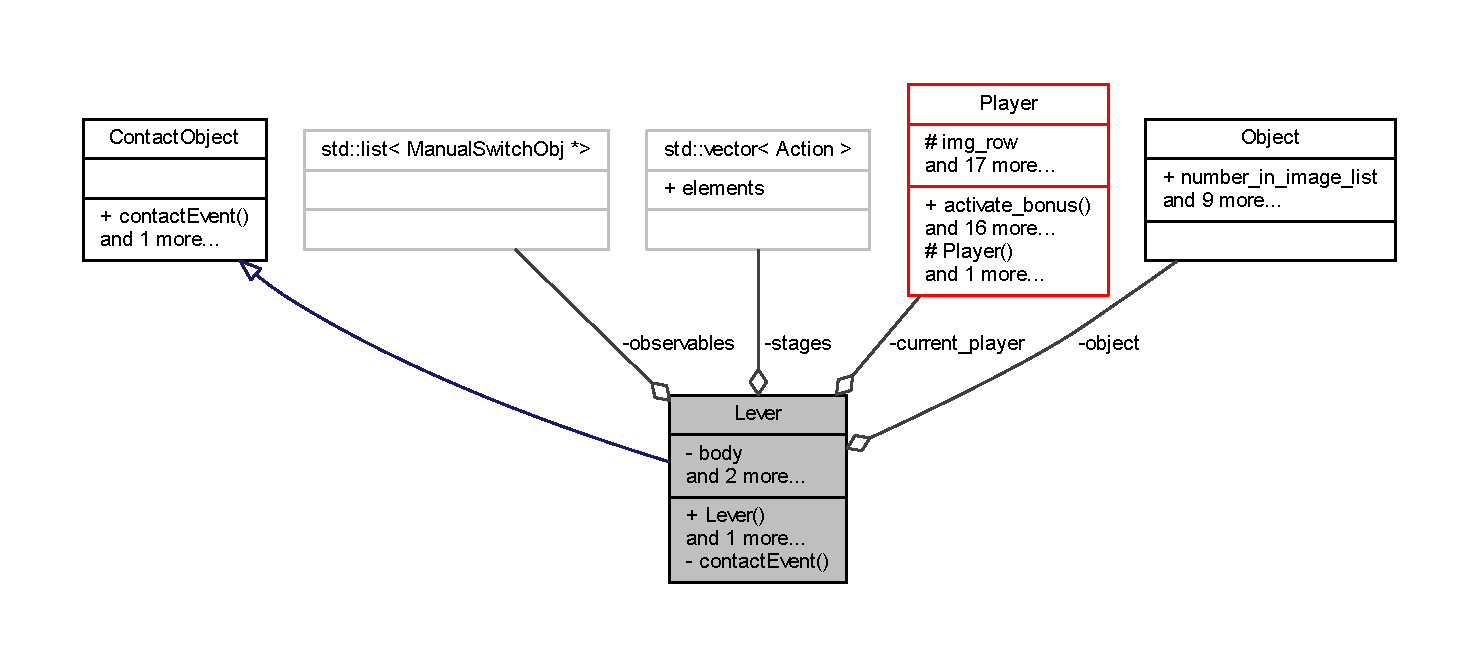
\includegraphics[width=350pt]{class_lever__coll__graph}
\end{center}
\end{figure}
\subsection*{Public Member Functions}
\begin{DoxyCompactItemize}
\item 
\hyperlink{class_lever_a2b4dd6cea65837c09711dda3d02d7cae}{Lever} (std\+::list$<$ \hyperlink{class_manual_switch_obj}{Manual\+Switch\+Obj} $\ast$$>$ \+\_\+observables, bool \+\_\+repeat\+\_\+allowed, b2\+Body $\ast$\+\_\+body, \hyperlink{class_object}{Object} $\ast$\+\_\+object, \hyperlink{class_player}{Player} $\ast$$\ast$\+\_\+current\+\_\+player, std\+::vector$<$ \hyperlink{_manual_switch_obj_8h_a8bb1ef53467e4f61410d12822d922498}{Action} $>$ \+\_\+stages)
\begin{DoxyCompactList}\small\item\em Defined constructor for this class. \end{DoxyCompactList}\item 
\mbox{\Hypertarget{class_lever_a0aafb7fa0e219a59362cfdbdc30f6203}\label{class_lever_a0aafb7fa0e219a59362cfdbdc30f6203}} 
void \hyperlink{class_lever_a0aafb7fa0e219a59362cfdbdc30f6203}{activate} ()
\begin{DoxyCompactList}\small\item\em causes the lever try to send next command to observables objects \end{DoxyCompactList}\end{DoxyCompactItemize}
\subsection*{Private Member Functions}
\begin{DoxyCompactItemize}
\item 
\mbox{\Hypertarget{class_lever_a08d617d4aad99c811df6013648843d8b}\label{class_lever_a08d617d4aad99c811df6013648843d8b}} 
void \hyperlink{class_lever_a08d617d4aad99c811df6013648843d8b}{contact\+Event} (b2\+Contact $\ast$contact, bool is\+\_\+begin)
\begin{DoxyCompactList}\small\item\em inherited from \hyperlink{class_contact_object}{Contact\+Object} class \end{DoxyCompactList}\end{DoxyCompactItemize}
\subsection*{Private Attributes}
\begin{DoxyCompactItemize}
\item 
\mbox{\Hypertarget{class_lever_aa063d5dab7eefeee48b93c0ea694bb42}\label{class_lever_aa063d5dab7eefeee48b93c0ea694bb42}} 
b2\+Body $\ast$ \hyperlink{class_lever_aa063d5dab7eefeee48b93c0ea694bb42}{body}
\begin{DoxyCompactList}\small\item\em pointer to the box2d body assigned to this lever \end{DoxyCompactList}\item 
\mbox{\Hypertarget{class_lever_aee2d6a9e2fc7ff31a9d8eea2f98b7e32}\label{class_lever_aee2d6a9e2fc7ff31a9d8eea2f98b7e32}} 
\hyperlink{class_object}{Object} $\ast$ \hyperlink{class_lever_aee2d6a9e2fc7ff31a9d8eea2f98b7e32}{object}
\begin{DoxyCompactList}\small\item\em pointer to the \hyperlink{class_object}{Object} class assigned to this lever \end{DoxyCompactList}\item 
\mbox{\Hypertarget{class_lever_ac710b732ab842d55f84488f9d88e325b}\label{class_lever_ac710b732ab842d55f84488f9d88e325b}} 
\hyperlink{class_player}{Player} $\ast$$\ast$ \hyperlink{class_lever_ac710b732ab842d55f84488f9d88e325b}{current\+\_\+player}
\begin{DoxyCompactList}\small\item\em pointer to the pointer containing infofmation about current active hero \end{DoxyCompactList}\item 
\mbox{\Hypertarget{class_lever_a8352c41d4452bf72a3f7d4dded03598c}\label{class_lever_a8352c41d4452bf72a3f7d4dded03598c}} 
std\+::vector$<$ \hyperlink{_manual_switch_obj_8h_a8bb1ef53467e4f61410d12822d922498}{Action} $>$ \hyperlink{class_lever_a8352c41d4452bf72a3f7d4dded03598c}{stages}
\begin{DoxyCompactList}\small\item\em vector of stages(commands) through which observables objects should pass \end{DoxyCompactList}\item 
\mbox{\Hypertarget{class_lever_ae7161c7fb8bc611f7d4cc3525d406e81}\label{class_lever_ae7161c7fb8bc611f7d4cc3525d406e81}} 
std\+::list$<$ \hyperlink{class_manual_switch_obj}{Manual\+Switch\+Obj} $\ast$ $>$ \hyperlink{class_lever_ae7161c7fb8bc611f7d4cc3525d406e81}{observables}
\begin{DoxyCompactList}\small\item\em list of observables objects \end{DoxyCompactList}\item 
\mbox{\Hypertarget{class_lever_a0a44f2d62a5ebc3bb5ae4aaed55076fb}\label{class_lever_a0a44f2d62a5ebc3bb5ae4aaed55076fb}} 
int \hyperlink{class_lever_a0a44f2d62a5ebc3bb5ae4aaed55076fb}{stage\+\_\+iter}
\begin{DoxyCompactList}\small\item\em number current stage from stages vector \end{DoxyCompactList}\item 
\mbox{\Hypertarget{class_lever_a8c464b1b28d5978e48bc3bc85a8cb67d}\label{class_lever_a8c464b1b28d5978e48bc3bc85a8cb67d}} 
bool \hyperlink{class_lever_a8c464b1b28d5978e48bc3bc85a8cb67d}{repeat\+\_\+allowed}
\begin{DoxyCompactList}\small\item\em determines whether it is possible to send next command to the observables objects when they doesn\textquotesingle{}t complete previous action\+: \textquotesingle{}true\textquotesingle{} -\/ possible; \textquotesingle{}false\textquotesingle{} -\/ impossible \end{DoxyCompactList}\end{DoxyCompactItemize}


\subsection{Detailed Description}
Special sensor that can be activated only by hero. 

\begin{DoxyAuthor}{Author}
Vasily 
\end{DoxyAuthor}
\begin{DoxyVersion}{Version}
1.\+0 
\end{DoxyVersion}
\begin{DoxyDate}{Date}
June 2017 
\end{DoxyDate}


\subsection{Constructor \& Destructor Documentation}
\mbox{\Hypertarget{class_lever_a2b4dd6cea65837c09711dda3d02d7cae}\label{class_lever_a2b4dd6cea65837c09711dda3d02d7cae}} 
\index{Lever@{Lever}!Lever@{Lever}}
\index{Lever@{Lever}!Lever@{Lever}}
\subsubsection{\texorpdfstring{Lever()}{Lever()}}
{\footnotesize\ttfamily Lever\+::\+Lever (\begin{DoxyParamCaption}\item[{std\+::list$<$ \hyperlink{class_manual_switch_obj}{Manual\+Switch\+Obj} $\ast$$>$}]{\+\_\+observables,  }\item[{bool}]{\+\_\+repeat\+\_\+allowed,  }\item[{b2\+Body $\ast$}]{\+\_\+body,  }\item[{\hyperlink{class_object}{Object} $\ast$}]{\+\_\+object,  }\item[{\hyperlink{class_player}{Player} $\ast$$\ast$}]{\+\_\+current\+\_\+player,  }\item[{std\+::vector$<$ \hyperlink{_manual_switch_obj_8h_a8bb1ef53467e4f61410d12822d922498}{Action} $>$}]{\+\_\+stages }\end{DoxyParamCaption})}



Defined constructor for this class. 


\begin{DoxyParams}{Parameters}
{\em \+\_\+observables} & list of observables objects \\
\hline
{\em \+\_\+repeat\+\_\+allowed} & determines whether it is possible to send next command to the observables objects when they doesn\textquotesingle{}t complete previous action\+: \textquotesingle{}true\textquotesingle{} -\/ possible; \textquotesingle{}false\textquotesingle{} -\/ impossible \\
\hline
{\em \+\_\+body} & pointer to the box2d body assigned to this entity \\
\hline
{\em \+\_\+object} & pointer to the \hyperlink{class_object}{Object} class assigned to this entity \\
\hline
{\em \+\_\+current\+\_\+player} & pointer to the pointer containing infofmation about current active hero \\
\hline
{\em \+\_\+stages} & vector of stages(commands) through which observables objects should pass \\
\hline
\end{DoxyParams}


The documentation for this class was generated from the following files\+:\begin{DoxyCompactItemize}
\item 
\hyperlink{_lever_8h}{Lever.\+h}\item 
Lever.\+cpp\end{DoxyCompactItemize}

\hypertarget{class_local_menu}{}\section{Local\+Menu Class Reference}
\label{class_local_menu}\index{Local\+Menu@{Local\+Menu}}


\char`\"{}\+Local menu\char`\"{} screen  




{\ttfamily \#include $<$Local\+Menu.\+h$>$}



Collaboration diagram for Local\+Menu\+:\nopagebreak
\begin{figure}[H]
\begin{center}
\leavevmode
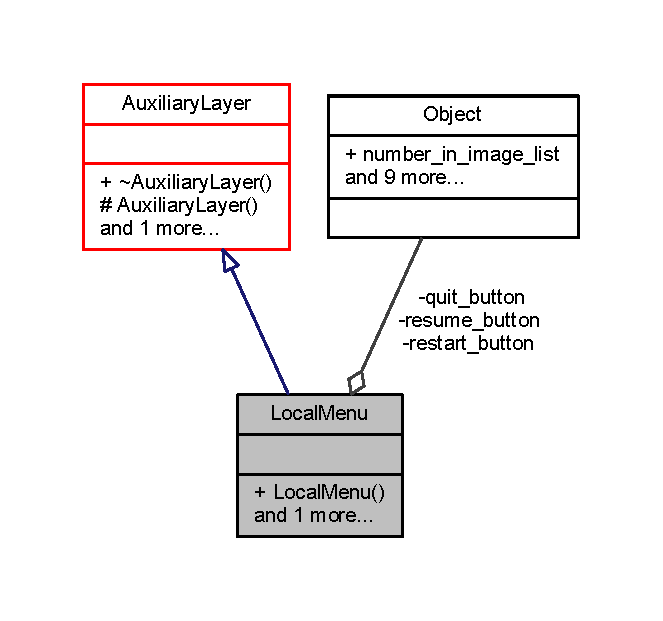
\includegraphics[width=318pt]{class_local_menu__coll__graph}
\end{center}
\end{figure}
\subsection*{Public Member Functions}
\begin{DoxyCompactItemize}
\item 
\mbox{\Hypertarget{class_local_menu_a5e20a17475cf56d630a80e6972b44261}\label{class_local_menu_a5e20a17475cf56d630a80e6972b44261}} 
\hyperlink{class_local_menu_a5e20a17475cf56d630a80e6972b44261}{Local\+Menu} ()
\begin{DoxyCompactList}\small\item\em Default constructor. \end{DoxyCompactList}\item 
void \hyperlink{class_local_menu_ad6db1f0ae5757a4e25269d40f6e369af}{smth\+Happend} (\hyperlink{_events_8h_af60e00b78607064c5be6aa9397ea49c1}{Events} what\+\_\+happened)
\begin{DoxyCompactList}\small\item\em Listener of player action. \end{DoxyCompactList}\end{DoxyCompactItemize}
\subsection*{Private Attributes}
\begin{DoxyCompactItemize}
\item 
\mbox{\Hypertarget{class_local_menu_ae41e7879af3597e9813855ead692ac54}\label{class_local_menu_ae41e7879af3597e9813855ead692ac54}} 
\hyperlink{class_object}{Object} $\ast$ \hyperlink{class_local_menu_ae41e7879af3597e9813855ead692ac54}{restart\+\_\+button}
\begin{DoxyCompactList}\small\item\em Pointer to object contain button \char`\"{}\+Restart\char`\"{}. \end{DoxyCompactList}\item 
\mbox{\Hypertarget{class_local_menu_a8a16de3ea6b9bb26b14cbbbaac7ff877}\label{class_local_menu_a8a16de3ea6b9bb26b14cbbbaac7ff877}} 
\hyperlink{class_object}{Object} $\ast$ \hyperlink{class_local_menu_a8a16de3ea6b9bb26b14cbbbaac7ff877}{quit\+\_\+button}
\begin{DoxyCompactList}\small\item\em Pointer to object contain button \char`\"{}\+Quit\char`\"{}. \end{DoxyCompactList}\item 
\mbox{\Hypertarget{class_local_menu_ad7c83497bd1737707763c9350d99ab44}\label{class_local_menu_ad7c83497bd1737707763c9350d99ab44}} 
\hyperlink{class_object}{Object} $\ast$ \hyperlink{class_local_menu_ad7c83497bd1737707763c9350d99ab44}{resume\+\_\+button}
\begin{DoxyCompactList}\small\item\em Pointer to object contain button \char`\"{}\+Resume\char`\"{}. \end{DoxyCompactList}\end{DoxyCompactItemize}
\subsection*{Additional Inherited Members}


\subsection{Detailed Description}
\char`\"{}\+Local menu\char`\"{} screen 

\begin{DoxyAuthor}{Author}
Vasily 
\end{DoxyAuthor}
\begin{DoxyVersion}{Version}
1.\+0 
\end{DoxyVersion}
\begin{DoxyDate}{Date}
June 2017
\end{DoxyDate}
Stores information needed to display \char`\"{}\+Local menu\char`\"{} screen at the level 

\subsection{Member Function Documentation}
\mbox{\Hypertarget{class_local_menu_ad6db1f0ae5757a4e25269d40f6e369af}\label{class_local_menu_ad6db1f0ae5757a4e25269d40f6e369af}} 
\index{Local\+Menu@{Local\+Menu}!smth\+Happend@{smth\+Happend}}
\index{smth\+Happend@{smth\+Happend}!Local\+Menu@{Local\+Menu}}
\subsubsection{\texorpdfstring{smth\+Happend()}{smthHappend()}}
{\footnotesize\ttfamily void Local\+Menu\+::smth\+Happend (\begin{DoxyParamCaption}\item[{\hyperlink{_events_8h_af60e00b78607064c5be6aa9397ea49c1}{Events}}]{what\+\_\+happened }\end{DoxyParamCaption})\hspace{0.3cm}{\ttfamily [virtual]}}



Listener of player action. 

Virtual method, inhereted from \hyperlink{class_layer}{Layer} class, which allow react to user action 
\begin{DoxyParams}{Parameters}
{\em what\+\_\+happened} & enum describing player action \\
\hline
\end{DoxyParams}


Implements \hyperlink{class_layer_a41318993a0f6c7ba3bc6d964f7802c10}{Layer}.



The documentation for this class was generated from the following files\+:\begin{DoxyCompactItemize}
\item 
\hyperlink{_local_menu_8h}{Local\+Menu.\+h}\item 
Local\+Menu.\+cpp\end{DoxyCompactItemize}

\hypertarget{class_main_menu}{}\section{Main\+Menu Class Reference}
\label{class_main_menu}\index{Main\+Menu@{Main\+Menu}}


\char`\"{}\+Main menu\char`\"{} screen  




{\ttfamily \#include $<$Main\+Menu.\+h$>$}



Collaboration diagram for Main\+Menu\+:
\nopagebreak
\begin{figure}[H]
\begin{center}
\leavevmode
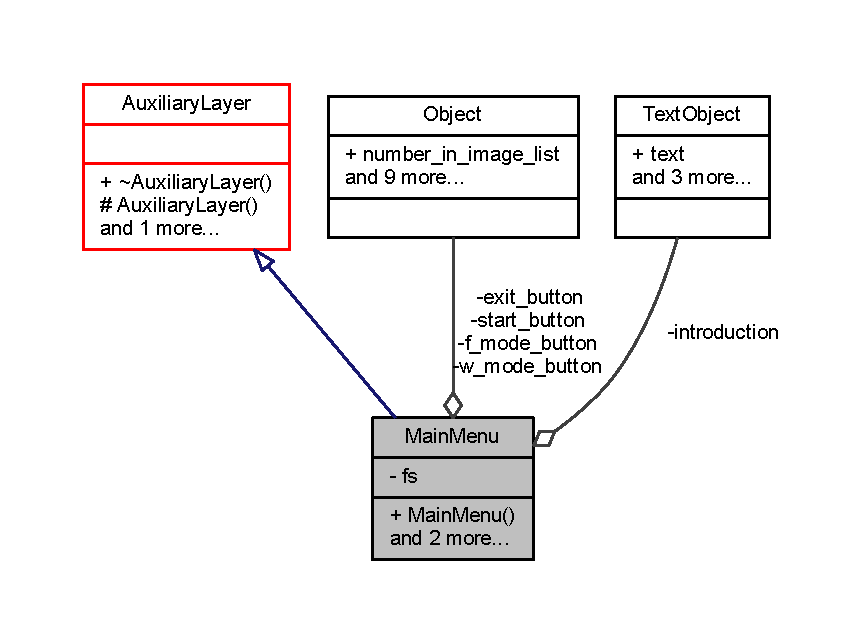
\includegraphics[width=350pt]{class_main_menu__coll__graph}
\end{center}
\end{figure}
\subsection*{Public Member Functions}
\begin{DoxyCompactItemize}
\item 
\mbox{\Hypertarget{class_main_menu_a53eecf9d5ffd094f54ac4193e7e57eaf}\label{class_main_menu_a53eecf9d5ffd094f54ac4193e7e57eaf}} 
\hyperlink{class_main_menu_a53eecf9d5ffd094f54ac4193e7e57eaf}{Main\+Menu} ()
\begin{DoxyCompactList}\small\item\em Default constructor. \end{DoxyCompactList}\item 
void \hyperlink{class_main_menu_aa4272e1cb2c70c23c869d301f2dd2110}{smth\+Happend} (\hyperlink{_events_8h_af60e00b78607064c5be6aa9397ea49c1}{Events} what\+\_\+happened)
\begin{DoxyCompactList}\small\item\em Listener of player action. \end{DoxyCompactList}\item 
bool \hyperlink{class_main_menu_a9b8bc5319e82474ecc03ae19b52c4293}{is\+ContainsC} (double x, double y, \hyperlink{class_object}{Object} $\ast$button)
\begin{DoxyCompactList}\small\item\em Check the entry of a coordinate into an object (button default) \end{DoxyCompactList}\end{DoxyCompactItemize}
\subsection*{Private Attributes}
\begin{DoxyCompactItemize}
\item 
\mbox{\Hypertarget{class_main_menu_a2202aa0a009aaa8593766768934f2ed2}\label{class_main_menu_a2202aa0a009aaa8593766768934f2ed2}} 
\hyperlink{class_text_object}{Text\+Object} \hyperlink{class_main_menu_a2202aa0a009aaa8593766768934f2ed2}{introduction}
\begin{DoxyCompactList}\small\item\em Title of the game. \end{DoxyCompactList}\item 
\mbox{\Hypertarget{class_main_menu_a49c056eefba301d78aff8840fd376cc7}\label{class_main_menu_a49c056eefba301d78aff8840fd376cc7}} 
\hyperlink{class_object}{Object} $\ast$ \hyperlink{class_main_menu_a49c056eefba301d78aff8840fd376cc7}{start\+\_\+button}
\begin{DoxyCompactList}\small\item\em Pointer to object contain button \char`\"{}\+Start\char`\"{}. \end{DoxyCompactList}\item 
\mbox{\Hypertarget{class_main_menu_aaa1f9030ef6aedef97961b5da7dde06a}\label{class_main_menu_aaa1f9030ef6aedef97961b5da7dde06a}} 
\hyperlink{class_object}{Object} $\ast$ \hyperlink{class_main_menu_aaa1f9030ef6aedef97961b5da7dde06a}{exit\+\_\+button}
\begin{DoxyCompactList}\small\item\em Pointer to object contain button \char`\"{}\+Exit\char`\"{}. \end{DoxyCompactList}\item 
\mbox{\Hypertarget{class_main_menu_a6de7ff52312a688a795acbe4baddb781}\label{class_main_menu_a6de7ff52312a688a795acbe4baddb781}} 
\hyperlink{class_object}{Object} $\ast$ \hyperlink{class_main_menu_a6de7ff52312a688a795acbe4baddb781}{f\+\_\+mode\+\_\+button}
\begin{DoxyCompactList}\small\item\em Pointer to object contain button \char`\"{}\+Fullscreen\char`\"{}. \end{DoxyCompactList}\item 
\mbox{\Hypertarget{class_main_menu_a61f684f61f99383c58f4fc09c50b1f9d}\label{class_main_menu_a61f684f61f99383c58f4fc09c50b1f9d}} 
\hyperlink{class_object}{Object} $\ast$ \hyperlink{class_main_menu_a61f684f61f99383c58f4fc09c50b1f9d}{w\+\_\+mode\+\_\+button}
\begin{DoxyCompactList}\small\item\em Pointer to object contain button \char`\"{}\+Windowed\char`\"{}. \end{DoxyCompactList}\item 
bool \hyperlink{class_main_menu_a22890c1716e56c182b500088c13d7f34}{fs}
\begin{DoxyCompactList}\small\item\em Define which button active now. \end{DoxyCompactList}\end{DoxyCompactItemize}
\subsection*{Additional Inherited Members}


\subsection{Detailed Description}
\char`\"{}\+Main menu\char`\"{} screen 

\begin{DoxyAuthor}{Author}
Vasily 
\end{DoxyAuthor}
\begin{DoxyVersion}{Version}
1.\+0 
\end{DoxyVersion}
\begin{DoxyDate}{Date}
June 2017
\end{DoxyDate}
Stores information needed to display \char`\"{}\+Main menu\char`\"{} 

\subsection{Member Function Documentation}
\mbox{\Hypertarget{class_main_menu_a9b8bc5319e82474ecc03ae19b52c4293}\label{class_main_menu_a9b8bc5319e82474ecc03ae19b52c4293}} 
\index{Main\+Menu@{Main\+Menu}!is\+ContainsC@{is\+ContainsC}}
\index{is\+ContainsC@{is\+ContainsC}!Main\+Menu@{Main\+Menu}}
\subsubsection{\texorpdfstring{is\+Contains\+C()}{isContainsC()}}
{\footnotesize\ttfamily bool Main\+Menu\+::is\+ContainsC (\begin{DoxyParamCaption}\item[{double}]{x,  }\item[{double}]{y,  }\item[{\hyperlink{class_object}{Object} $\ast$}]{button }\end{DoxyParamCaption})}



Check the entry of a coordinate into an object (button default) 

Special function to dynamic object which origin is their center, not an left-\/top corner (diff. from is\+Contains in \hyperlink{class_auxiliary_layer}{Auxiliary\+Layer} class) 
\begin{DoxyParams}{Parameters}
{\em x} & x coordinate \\
\hline
{\em y} & y coordinate \\
\hline
{\em button} & object to check \\
\hline
\end{DoxyParams}
\mbox{\Hypertarget{class_main_menu_aa4272e1cb2c70c23c869d301f2dd2110}\label{class_main_menu_aa4272e1cb2c70c23c869d301f2dd2110}} 
\index{Main\+Menu@{Main\+Menu}!smth\+Happend@{smth\+Happend}}
\index{smth\+Happend@{smth\+Happend}!Main\+Menu@{Main\+Menu}}
\subsubsection{\texorpdfstring{smth\+Happend()}{smthHappend()}}
{\footnotesize\ttfamily void Main\+Menu\+::smth\+Happend (\begin{DoxyParamCaption}\item[{\hyperlink{_events_8h_af60e00b78607064c5be6aa9397ea49c1}{Events}}]{what\+\_\+happened }\end{DoxyParamCaption})\hspace{0.3cm}{\ttfamily [virtual]}}



Listener of player action. 

Virtual method, inhereted from \hyperlink{class_layer}{Layer} class, which allow react to user action 
\begin{DoxyParams}{Parameters}
{\em what\+\_\+happened} & enum describing player action \\
\hline
\end{DoxyParams}


Implements \hyperlink{class_layer_a41318993a0f6c7ba3bc6d964f7802c10}{Layer}.



\subsection{Member Data Documentation}
\mbox{\Hypertarget{class_main_menu_a22890c1716e56c182b500088c13d7f34}\label{class_main_menu_a22890c1716e56c182b500088c13d7f34}} 
\index{Main\+Menu@{Main\+Menu}!fs@{fs}}
\index{fs@{fs}!Main\+Menu@{Main\+Menu}}
\subsubsection{\texorpdfstring{fs}{fs}}
{\footnotesize\ttfamily bool Main\+Menu\+::fs\hspace{0.3cm}{\ttfamily [private]}}



Define which button active now. 


\begin{DoxyParams}{Parameters}
{\em false} & \char`\"{}\+Windowed\char`\"{} button active \\
\hline
{\em true} & \char`\"{}\+Fullscreen\char`\"{} button active \\
\hline
\end{DoxyParams}


The documentation for this class was generated from the following files\+:\begin{DoxyCompactItemize}
\item 
\hyperlink{_main_menu_8h}{Main\+Menu.\+h}\item 
Main\+Menu.\+cpp\end{DoxyCompactItemize}

\hypertarget{class_manual_platform}{}\section{Manual\+Platform Class Reference}
\label{class_manual_platform}\index{Manual\+Platform@{Manual\+Platform}}


\hyperlink{class_platform}{Platform} that can be activated by the sensor.  




{\ttfamily \#include $<$Manual\+Platform.\+h$>$}



Collaboration diagram for Manual\+Platform\+:\nopagebreak
\begin{figure}[H]
\begin{center}
\leavevmode
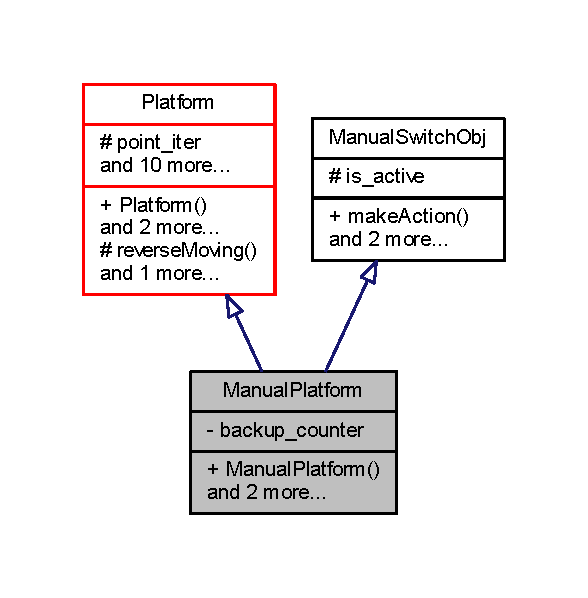
\includegraphics[width=282pt]{class_manual_platform__coll__graph}
\end{center}
\end{figure}
\subsection*{Public Member Functions}
\begin{DoxyCompactItemize}
\item 
\hyperlink{class_manual_platform_a0192ef683b0f19b93bd238af98f8ce51}{Manual\+Platform} (int \+\_\+level\+\_\+width, int \+\_\+level\+\_\+height, b2\+Body $\ast$\+\_\+body, \hyperlink{class_object}{Object} $\ast$\+\_\+object, std\+::vector$<$ std\+::pair$<$ double, double $>$$>$ traj\+\_\+coord, int \+\_\+fixed\+\_\+speed, bool \+\_\+is\+\_\+rounded, int \+\_\+node\+\_\+number)
\begin{DoxyCompactList}\small\item\em Defined constructor for this class. \end{DoxyCompactList}\item 
\mbox{\Hypertarget{class_manual_platform_ae77ccd8210c4ee32606b3475154325d4}\label{class_manual_platform_ae77ccd8210c4ee32606b3475154325d4}} 
void \hyperlink{class_manual_platform_ae77ccd8210c4ee32606b3475154325d4}{update} ()
\begin{DoxyCompactList}\small\item\em inherited from \hyperlink{class_platform}{Platform} class \end{DoxyCompactList}\item 
void \hyperlink{class_manual_platform_ad7ae2aac108330a84246e3337fb5af81}{make\+Action} (Action)
\begin{DoxyCompactList}\small\item\em causes the bridge to make some action \end{DoxyCompactList}\item 
b2\+Body $\ast$ \hyperlink{class_manual_platform_ad8afd5278a85a63f1b597a3851bfc65d}{get\+Body} ()
\item 
\hyperlink{class_object}{Object} $\ast$ \hyperlink{class_manual_platform_ad7deba6261f272ed530786e0f742b2f5}{get\+Object} ()
\end{DoxyCompactItemize}
\subsection*{Private Attributes}
\begin{DoxyCompactItemize}
\item 
\mbox{\Hypertarget{class_manual_platform_a8734cff028bd7e94fabc38be3f712534}\label{class_manual_platform_a8734cff028bd7e94fabc38be3f712534}} 
int \hyperlink{class_manual_platform_a8734cff028bd7e94fabc38be3f712534}{backup\+\_\+counter} = 0
\begin{DoxyCompactList}\small\item\em store backup of the current node of the trajectory for this platform \end{DoxyCompactList}\end{DoxyCompactItemize}
\subsection*{Additional Inherited Members}


\subsection{Detailed Description}
\hyperlink{class_platform}{Platform} that can be activated by the sensor. 

\begin{DoxyAuthor}{Author}
Vasily 
\end{DoxyAuthor}
\begin{DoxyVersion}{Version}
1.\+0 
\end{DoxyVersion}
\begin{DoxyDate}{Date}
June 2017 
\end{DoxyDate}


\subsection{Constructor \& Destructor Documentation}
\mbox{\Hypertarget{class_manual_platform_a0192ef683b0f19b93bd238af98f8ce51}\label{class_manual_platform_a0192ef683b0f19b93bd238af98f8ce51}} 
\index{Manual\+Platform@{Manual\+Platform}!Manual\+Platform@{Manual\+Platform}}
\index{Manual\+Platform@{Manual\+Platform}!Manual\+Platform@{Manual\+Platform}}
\subsubsection{\texorpdfstring{Manual\+Platform()}{ManualPlatform()}}
{\footnotesize\ttfamily Manual\+Platform\+::\+Manual\+Platform (\begin{DoxyParamCaption}\item[{int}]{\+\_\+level\+\_\+width,  }\item[{int}]{\+\_\+level\+\_\+height,  }\item[{b2\+Body $\ast$}]{\+\_\+body,  }\item[{\hyperlink{class_object}{Object} $\ast$}]{\+\_\+object,  }\item[{std\+::vector$<$ std\+::pair$<$ double, double $>$$>$}]{traj\+\_\+coord,  }\item[{int}]{\+\_\+fixed\+\_\+speed,  }\item[{bool}]{\+\_\+is\+\_\+rounded,  }\item[{int}]{\+\_\+node\+\_\+number }\end{DoxyParamCaption})}



Defined constructor for this class. 


\begin{DoxyParams}{Parameters}
{\em \+\_\+level\+\_\+width} & the width in pixels of this level \\
\hline
{\em \+\_\+level\+\_\+height} & the height in pixels of this level \\
\hline
{\em \+\_\+body} & pointer to the box2d body assigned to this platform \\
\hline
{\em \+\_\+object} & pointer to the \hyperlink{class_object}{Object} class assigned to this platform \\
\hline
{\em \+\_\+traj\+\_\+coord} & set of the trajectory coordinates for this platform \\
\hline
{\em \+\_\+fixed\+\_\+speed} & speed of the platform \\
\hline
{\em \+\_\+is\+\_\+rounded} & defines the shape of trajectory \textquotesingle{}true\textquotesingle{} -\/ closed \textquotesingle{}false\textquotesingle{} -\/ torn \\
\hline
{\em \+\_\+node\+\_\+number} & max number of trajectory nodes which platform passed before reverse moving or the stop \\
\hline
\end{DoxyParams}


\subsection{Member Function Documentation}
\mbox{\Hypertarget{class_manual_platform_ad8afd5278a85a63f1b597a3851bfc65d}\label{class_manual_platform_ad8afd5278a85a63f1b597a3851bfc65d}} 
\index{Manual\+Platform@{Manual\+Platform}!get\+Body@{get\+Body}}
\index{get\+Body@{get\+Body}!Manual\+Platform@{Manual\+Platform}}
\subsubsection{\texorpdfstring{get\+Body()}{getBody()}}
{\footnotesize\ttfamily b2\+Body $\ast$ Manual\+Platform\+::get\+Body (\begin{DoxyParamCaption}{ }\end{DoxyParamCaption})}

\begin{DoxyReturn}{Returns}
pointer to the box2d body assigned to this platform 
\end{DoxyReturn}
\mbox{\Hypertarget{class_manual_platform_ad7deba6261f272ed530786e0f742b2f5}\label{class_manual_platform_ad7deba6261f272ed530786e0f742b2f5}} 
\index{Manual\+Platform@{Manual\+Platform}!get\+Object@{get\+Object}}
\index{get\+Object@{get\+Object}!Manual\+Platform@{Manual\+Platform}}
\subsubsection{\texorpdfstring{get\+Object()}{getObject()}}
{\footnotesize\ttfamily \hyperlink{class_object}{Object} $\ast$ Manual\+Platform\+::get\+Object (\begin{DoxyParamCaption}{ }\end{DoxyParamCaption})}

\begin{DoxyReturn}{Returns}
pointer to the \hyperlink{class_object}{Object} class assigned to this platform 
\end{DoxyReturn}
\mbox{\Hypertarget{class_manual_platform_ad7ae2aac108330a84246e3337fb5af81}\label{class_manual_platform_ad7ae2aac108330a84246e3337fb5af81}} 
\index{Manual\+Platform@{Manual\+Platform}!make\+Action@{make\+Action}}
\index{make\+Action@{make\+Action}!Manual\+Platform@{Manual\+Platform}}
\subsubsection{\texorpdfstring{make\+Action()}{makeAction()}}
{\footnotesize\ttfamily void Manual\+Platform\+::make\+Action (\begin{DoxyParamCaption}\item[{Action}]{ }\end{DoxyParamCaption})\hspace{0.3cm}{\ttfamily [virtual]}}



causes the bridge to make some action 


\begin{DoxyParams}{Parameters}
{\em action} & what necessary to make (doesn\textquotesingle{}t matter; always Action\+::default is expected) \\
\hline
\end{DoxyParams}


Reimplemented from \hyperlink{class_manual_switch_obj}{Manual\+Switch\+Obj}.



The documentation for this class was generated from the following files\+:\begin{DoxyCompactItemize}
\item 
\hyperlink{_manual_platform_8h}{Manual\+Platform.\+h}\item 
Manual\+Platform.\+cpp\end{DoxyCompactItemize}

\hypertarget{class_manual_switch_obj}{}\section{Manual\+Switch\+Obj Class Reference}
\label{class_manual_switch_obj}\index{Manual\+Switch\+Obj@{Manual\+Switch\+Obj}}


Collaboration diagram for Manual\+Switch\+Obj\+:\nopagebreak
\begin{figure}[H]
\begin{center}
\leavevmode
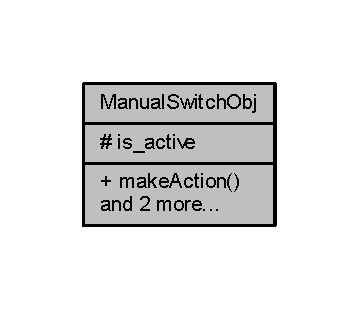
\includegraphics[width=172pt]{class_manual_switch_obj__coll__graph}
\end{center}
\end{figure}
\subsection*{Public Member Functions}
\begin{DoxyCompactItemize}
\item 
\mbox{\Hypertarget{class_manual_switch_obj_a138301db593d2b231bad0298a38e1680}\label{class_manual_switch_obj_a138301db593d2b231bad0298a38e1680}} 
virtual void {\bfseries make\+Action} (Action)
\item 
\mbox{\Hypertarget{class_manual_switch_obj_a4d6cc0a3de424ab6bf4665eeb0f639af}\label{class_manual_switch_obj_a4d6cc0a3de424ab6bf4665eeb0f639af}} 
virtual bool {\bfseries is\+Active} ()
\end{DoxyCompactItemize}
\subsection*{Protected Attributes}
\begin{DoxyCompactItemize}
\item 
\mbox{\Hypertarget{class_manual_switch_obj_aa1d16c8a1740f4dc3152470088154f97}\label{class_manual_switch_obj_aa1d16c8a1740f4dc3152470088154f97}} 
bool {\bfseries is\+\_\+active} = false
\end{DoxyCompactItemize}


The documentation for this class was generated from the following files\+:\begin{DoxyCompactItemize}
\item 
Manual\+Switch\+Obj.\+h\item 
Manual\+Switch\+Obj.\+cpp\end{DoxyCompactItemize}

\hypertarget{class_model}{}\section{Model Class Reference}
\label{class_model}\index{Model@{Model}}


Element-\/container in M\+VC structure.  




{\ttfamily \#include $<$Model.\+h$>$}



Collaboration diagram for Model\+:
\nopagebreak
\begin{figure}[H]
\begin{center}
\leavevmode
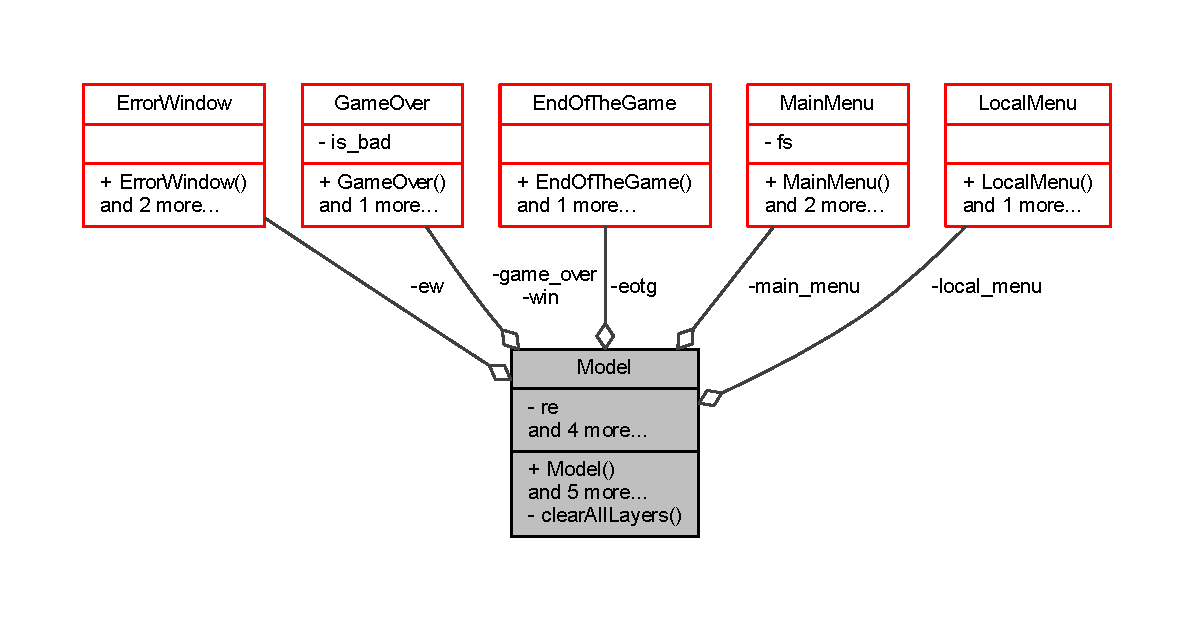
\includegraphics[width=350pt]{class_model__coll__graph}
\end{center}
\end{figure}
\subsection*{Public Member Functions}
\begin{DoxyCompactItemize}
\item 
\mbox{\Hypertarget{class_model_ae3b375de5f6df4faf74a95d64748e048}\label{class_model_ae3b375de5f6df4faf74a95d64748e048}} 
\hyperlink{class_model_ae3b375de5f6df4faf74a95d64748e048}{Model} ()
\begin{DoxyCompactList}\small\item\em Default constructor. \end{DoxyCompactList}\item 
void \hyperlink{class_model_a2b3b7cbe02e7cac025290136e4c11e54}{handle\+Event} (\hyperlink{_events_8h_af60e00b78607064c5be6aa9397ea49c1}{Events} event)
\begin{DoxyCompactList}\small\item\em causes \hyperlink{class_model}{Model} to react on \hyperlink{class_controller}{Controller} command \end{DoxyCompactList}\item 
\mbox{\Hypertarget{class_model_a8976f84f757eb3cd68b2aa7eeb5a345f}\label{class_model_a8976f84f757eb3cd68b2aa7eeb5a345f}} 
void \hyperlink{class_model_a8976f84f757eb3cd68b2aa7eeb5a345f}{update} ()
\begin{DoxyCompactList}\small\item\em causes \hyperlink{class_model}{Model} to update state \end{DoxyCompactList}\item 
\hyperlink{class_layer}{Layer} $\ast$ \hyperlink{class_model_acdaa9cd882c6f43d0ea60bc7010acfa2}{return\+Upper\+Layer} ()
\item 
\hyperlink{_events_8h_a387f1fc6b8a0efa93d5fed71c3d9c0bc}{Model\+Reaction} \hyperlink{class_model_aabbd887291832c912bc39487f829fb9a}{check\+Response} ()
\end{DoxyCompactItemize}
\subsection*{Private Member Functions}
\begin{DoxyCompactItemize}
\item 
\mbox{\Hypertarget{class_model_a3ad6a6d48906c82bc5ef7ff0ad00b190}\label{class_model_a3ad6a6d48906c82bc5ef7ff0ad00b190}} 
void \hyperlink{class_model_a3ad6a6d48906c82bc5ef7ff0ad00b190}{clear\+All\+Layers} ()
\begin{DoxyCompactList}\small\item\em clear stack \end{DoxyCompactList}\end{DoxyCompactItemize}
\subsection*{Private Attributes}
\begin{DoxyCompactItemize}
\item 
\mbox{\Hypertarget{class_model_af749476e8bdcd74948ebe837bd3dbfc8}\label{class_model_af749476e8bdcd74948ebe837bd3dbfc8}} 
\hyperlink{class_main_menu}{Main\+Menu} \hyperlink{class_model_af749476e8bdcd74948ebe837bd3dbfc8}{main\+\_\+menu}
\begin{DoxyCompactList}\small\item\em class with information needed to display \char`\"{}\+Main menu\char`\"{} \end{DoxyCompactList}\item 
\mbox{\Hypertarget{class_model_a905afcc359caed9ea41d17dfc5cef784}\label{class_model_a905afcc359caed9ea41d17dfc5cef784}} 
\hyperlink{class_game_over}{Game\+Over} \hyperlink{class_model_a905afcc359caed9ea41d17dfc5cef784}{game\+\_\+over}
\begin{DoxyCompactList}\small\item\em class with information needed to display \char`\"{}\+Game over\char`\"{} \end{DoxyCompactList}\item 
\mbox{\Hypertarget{class_model_a6e4433103b304e645fb85a6a9612b42e}\label{class_model_a6e4433103b304e645fb85a6a9612b42e}} 
\hyperlink{class_game_over}{Game\+Over} \hyperlink{class_model_a6e4433103b304e645fb85a6a9612b42e}{win}
\begin{DoxyCompactList}\small\item\em class with information needed to display \char`\"{}\+You win\char`\"{} \end{DoxyCompactList}\item 
\mbox{\Hypertarget{class_model_a53a6421a918ea8fab218d6eb7bc69119}\label{class_model_a53a6421a918ea8fab218d6eb7bc69119}} 
\hyperlink{class_local_menu}{Local\+Menu} \hyperlink{class_model_a53a6421a918ea8fab218d6eb7bc69119}{local\+\_\+menu}
\begin{DoxyCompactList}\small\item\em class with information needed to display \char`\"{}\+Local menu\char`\"{} \end{DoxyCompactList}\item 
\mbox{\Hypertarget{class_model_a44c5d8b7f91c4a3ea5fe5643a6fbf26e}\label{class_model_a44c5d8b7f91c4a3ea5fe5643a6fbf26e}} 
\hyperlink{class_end_of_the_game}{End\+Of\+The\+Game} \hyperlink{class_model_a44c5d8b7f91c4a3ea5fe5643a6fbf26e}{eotg}
\begin{DoxyCompactList}\small\item\em class with information needed to display \char`\"{}\+The end\char`\"{} \end{DoxyCompactList}\item 
\mbox{\Hypertarget{class_model_a7f547d436448e326441b8170c3ac7835}\label{class_model_a7f547d436448e326441b8170c3ac7835}} 
\hyperlink{class_error_window}{Error\+Window} \hyperlink{class_model_a7f547d436448e326441b8170c3ac7835}{ew}
\begin{DoxyCompactList}\small\item\em class with information needed to display \char`\"{}\+Error\char`\"{} \end{DoxyCompactList}\item 
\mbox{\Hypertarget{class_model_a72a4ba8da86e13263867c7e4e1cb9205}\label{class_model_a72a4ba8da86e13263867c7e4e1cb9205}} 
int \hyperlink{class_model_a72a4ba8da86e13263867c7e4e1cb9205}{current\+\_\+level}
\begin{DoxyCompactList}\small\item\em current level number among all levels in the list \end{DoxyCompactList}\item 
\mbox{\Hypertarget{class_model_a357abb457c3e8bf987dce2418c6f09b2}\label{class_model_a357abb457c3e8bf987dce2418c6f09b2}} 
std\+::vector$<$ std\+::string $>$ \hyperlink{class_model_a357abb457c3e8bf987dce2418c6f09b2}{level\+\_\+dir}
\begin{DoxyCompactList}\small\item\em vector with paths to images file \end{DoxyCompactList}\item 
\mbox{\Hypertarget{class_model_a1450c4773eee836985f551c288490bf4}\label{class_model_a1450c4773eee836985f551c288490bf4}} 
std\+::vector$<$ std\+::string $>$ \hyperlink{class_model_a1450c4773eee836985f551c288490bf4}{level\+\_\+names}
\begin{DoxyCompactList}\small\item\em vector with paths to the level file \end{DoxyCompactList}\item 
\mbox{\Hypertarget{class_model_ae25f86a150bc0b5c146ebd39567eea2f}\label{class_model_ae25f86a150bc0b5c146ebd39567eea2f}} 
std\+::stack$<$ \hyperlink{class_layer}{Layer} $\ast$ $>$ \hyperlink{class_model_ae25f86a150bc0b5c146ebd39567eea2f}{layers\+\_\+list}
\begin{DoxyCompactList}\small\item\em stack for game-\/state managment (react only top \hyperlink{class_layer}{Layer}) \end{DoxyCompactList}\end{DoxyCompactItemize}


\subsection{Detailed Description}
Element-\/container in M\+VC structure. 

\begin{DoxyAuthor}{Author}
Vasily 
\end{DoxyAuthor}
\begin{DoxyVersion}{Version}
1.\+0 
\end{DoxyVersion}
\begin{DoxyDate}{Date}
June 2017
\end{DoxyDate}
Contain necessary information and change state depending on controller commands 

\subsection{Member Function Documentation}
\mbox{\Hypertarget{class_model_aabbd887291832c912bc39487f829fb9a}\label{class_model_aabbd887291832c912bc39487f829fb9a}} 
\index{Model@{Model}!check\+Response@{check\+Response}}
\index{check\+Response@{check\+Response}!Model@{Model}}
\subsubsection{\texorpdfstring{check\+Response()}{checkResponse()}}
{\footnotesize\ttfamily \hyperlink{_events_8h_a387f1fc6b8a0efa93d5fed71c3d9c0bc}{Model\+Reaction} Model\+::check\+Response (\begin{DoxyParamCaption}{ }\end{DoxyParamCaption})}

\begin{DoxyReturn}{Returns}
reaction of the model to the last \hyperlink{class_controller}{Controller} command or update action 
\end{DoxyReturn}
\mbox{\Hypertarget{class_model_a2b3b7cbe02e7cac025290136e4c11e54}\label{class_model_a2b3b7cbe02e7cac025290136e4c11e54}} 
\index{Model@{Model}!handle\+Event@{handle\+Event}}
\index{handle\+Event@{handle\+Event}!Model@{Model}}
\subsubsection{\texorpdfstring{handle\+Event()}{handleEvent()}}
{\footnotesize\ttfamily void Model\+::handle\+Event (\begin{DoxyParamCaption}\item[{\hyperlink{_events_8h_af60e00b78607064c5be6aa9397ea49c1}{Events}}]{event }\end{DoxyParamCaption})}



causes \hyperlink{class_model}{Model} to react on \hyperlink{class_controller}{Controller} command 


\begin{DoxyParams}{Parameters}
{\em event} & \hyperlink{class_controller}{Controller} command in enum Events form \\
\hline
\end{DoxyParams}
\mbox{\Hypertarget{class_model_acdaa9cd882c6f43d0ea60bc7010acfa2}\label{class_model_acdaa9cd882c6f43d0ea60bc7010acfa2}} 
\index{Model@{Model}!return\+Upper\+Layer@{return\+Upper\+Layer}}
\index{return\+Upper\+Layer@{return\+Upper\+Layer}!Model@{Model}}
\subsubsection{\texorpdfstring{return\+Upper\+Layer()}{returnUpperLayer()}}
{\footnotesize\ttfamily \hyperlink{class_layer}{Layer} $\ast$ Model\+::return\+Upper\+Layer (\begin{DoxyParamCaption}{ }\end{DoxyParamCaption})}

\begin{DoxyReturn}{Returns}
top layer at \textquotesingle{}layers\+\_\+list\textquotesingle{} 
\end{DoxyReturn}


The documentation for this class was generated from the following files\+:\begin{DoxyCompactItemize}
\item 
\hyperlink{_model_8h}{Model.\+h}\item 
Model.\+cpp\end{DoxyCompactItemize}

\hypertarget{struct_mouse_click_coordinates}{}\section{Mouse\+Click\+Coordinates Struct Reference}
\label{struct_mouse_click_coordinates}\index{Mouse\+Click\+Coordinates@{Mouse\+Click\+Coordinates}}


last registered mouse click coordinates  




{\ttfamily \#include $<$Events.\+h$>$}



Collaboration diagram for Mouse\+Click\+Coordinates\+:\nopagebreak
\begin{figure}[H]
\begin{center}
\leavevmode
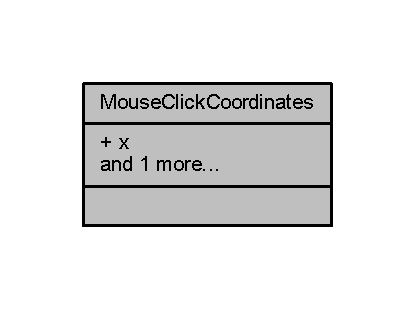
\includegraphics[width=199pt]{struct_mouse_click_coordinates__coll__graph}
\end{center}
\end{figure}
\subsection*{Static Public Attributes}
\begin{DoxyCompactItemize}
\item 
\mbox{\Hypertarget{struct_mouse_click_coordinates_ae2d7c0c719bbe09164c3650819dae696}\label{struct_mouse_click_coordinates_ae2d7c0c719bbe09164c3650819dae696}} 
static double \hyperlink{struct_mouse_click_coordinates_ae2d7c0c719bbe09164c3650819dae696}{x} = 0
\begin{DoxyCompactList}\small\item\em x coordinates \end{DoxyCompactList}\item 
\mbox{\Hypertarget{struct_mouse_click_coordinates_a093e1fd64d4009d358b00c1e58f20997}\label{struct_mouse_click_coordinates_a093e1fd64d4009d358b00c1e58f20997}} 
static double \hyperlink{struct_mouse_click_coordinates_a093e1fd64d4009d358b00c1e58f20997}{y} = 0
\begin{DoxyCompactList}\small\item\em y coordinates \end{DoxyCompactList}\end{DoxyCompactItemize}


\subsection{Detailed Description}
last registered mouse click coordinates 

\begin{DoxyAuthor}{Author}
Vasily 
\end{DoxyAuthor}
\begin{DoxyVersion}{Version}
1.\+0 
\end{DoxyVersion}
\begin{DoxyDate}{Date}
June 2017 
\end{DoxyDate}


The documentation for this struct was generated from the following files\+:\begin{DoxyCompactItemize}
\item 
\hyperlink{_events_8h}{Events.\+h}\item 
Events.\+cpp\end{DoxyCompactItemize}

\hypertarget{class_my_contact_listener}{}\section{My\+Contact\+Listener Class Reference}
\label{class_my_contact_listener}\index{My\+Contact\+Listener@{My\+Contact\+Listener}}


Override for standart box2d Contact\+Listener.  




{\ttfamily \#include $<$Contact\+Listener.\+h$>$}



Collaboration diagram for My\+Contact\+Listener\+:\nopagebreak
\begin{figure}[H]
\begin{center}
\leavevmode
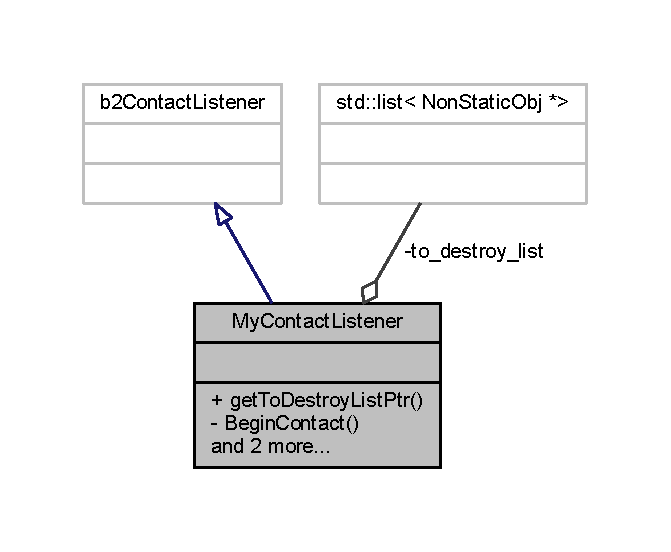
\includegraphics[width=322pt]{class_my_contact_listener__coll__graph}
\end{center}
\end{figure}
\subsection*{Public Member Functions}
\begin{DoxyCompactItemize}
\item 
std\+::list$<$ \hyperlink{class_non_static_obj}{Non\+Static\+Obj} $\ast$ $>$ $\ast$ \hyperlink{class_my_contact_listener_a3e414c674f98a2f35e2c894923d045b2}{get\+To\+Destroy\+List\+Ptr} ()
\end{DoxyCompactItemize}
\subsection*{Private Member Functions}
\begin{DoxyCompactItemize}
\item 
\mbox{\Hypertarget{class_my_contact_listener_abad225bec15c17598d20da175c169495}\label{class_my_contact_listener_abad225bec15c17598d20da175c169495}} 
void \hyperlink{class_my_contact_listener_abad225bec15c17598d20da175c169495}{Begin\+Contact} (b2\+Contact $\ast$contact)
\begin{DoxyCompactList}\small\item\em Override standart box2d function (see box2d man) \end{DoxyCompactList}\item 
\mbox{\Hypertarget{class_my_contact_listener_aa28063f833c2bf6162b044c03474436d}\label{class_my_contact_listener_aa28063f833c2bf6162b044c03474436d}} 
void \hyperlink{class_my_contact_listener_aa28063f833c2bf6162b044c03474436d}{End\+Contact} (b2\+Contact $\ast$contact)
\begin{DoxyCompactList}\small\item\em Override standart box2d function (see box2d man) \end{DoxyCompactList}\item 
\mbox{\Hypertarget{class_my_contact_listener_a691495aee67681d73d94c91e7c7a4df6}\label{class_my_contact_listener_a691495aee67681d73d94c91e7c7a4df6}} 
void \hyperlink{class_my_contact_listener_a691495aee67681d73d94c91e7c7a4df6}{Post\+Solve} (b2\+Contact $\ast$contact, const b2\+Contact\+Impulse $\ast$impulse)
\begin{DoxyCompactList}\small\item\em Override standart box2d function (see box2d man) \end{DoxyCompactList}\end{DoxyCompactItemize}
\subsection*{Private Attributes}
\begin{DoxyCompactItemize}
\item 
\mbox{\Hypertarget{class_my_contact_listener_a41da507e8c150d1898d73172e4e3f916}\label{class_my_contact_listener_a41da507e8c150d1898d73172e4e3f916}} 
std\+::list$<$ \hyperlink{class_non_static_obj}{Non\+Static\+Obj} $\ast$ $>$ \hyperlink{class_my_contact_listener_a41da507e8c150d1898d73172e4e3f916}{to\+\_\+destroy\+\_\+list}
\begin{DoxyCompactList}\small\item\em List, containing pointer level objects, which will be destroy after the end of box2d world simulation at the next update iteration. \end{DoxyCompactList}\end{DoxyCompactItemize}


\subsection{Detailed Description}
Override for standart box2d Contact\+Listener. 

\begin{DoxyAuthor}{Author}
Vasily 
\end{DoxyAuthor}
\begin{DoxyVersion}{Version}
1.\+0 
\end{DoxyVersion}
\begin{DoxyDate}{Date}
June 2017 
\end{DoxyDate}


\subsection{Member Function Documentation}
\mbox{\Hypertarget{class_my_contact_listener_a3e414c674f98a2f35e2c894923d045b2}\label{class_my_contact_listener_a3e414c674f98a2f35e2c894923d045b2}} 
\index{My\+Contact\+Listener@{My\+Contact\+Listener}!get\+To\+Destroy\+List\+Ptr@{get\+To\+Destroy\+List\+Ptr}}
\index{get\+To\+Destroy\+List\+Ptr@{get\+To\+Destroy\+List\+Ptr}!My\+Contact\+Listener@{My\+Contact\+Listener}}
\subsubsection{\texorpdfstring{get\+To\+Destroy\+List\+Ptr()}{getToDestroyListPtr()}}
{\footnotesize\ttfamily std\+::list$<$ \hyperlink{class_non_static_obj}{Non\+Static\+Obj} $\ast$ $>$ $\ast$ My\+Contact\+Listener\+::get\+To\+Destroy\+List\+Ptr (\begin{DoxyParamCaption}{ }\end{DoxyParamCaption})}

\begin{DoxyReturn}{Returns}
pointer to the \textquotesingle{}to\+\_\+destroy\+\_\+list\textquotesingle{} 
\end{DoxyReturn}


The documentation for this class was generated from the following files\+:\begin{DoxyCompactItemize}
\item 
\hyperlink{_contact_listener_8h}{Contact\+Listener.\+h}\item 
Contact\+Listener.\+cpp\end{DoxyCompactItemize}

\hypertarget{class_non_static_obj}{}\section{Non\+Static\+Obj Class Reference}
\label{class_non_static_obj}\index{Non\+Static\+Obj@{Non\+Static\+Obj}}


Typical object (an entity) that participates in physics simulation.  




{\ttfamily \#include $<$Non\+Static\+Obj.\+h$>$}



Collaboration diagram for Non\+Static\+Obj\+:
\nopagebreak
\begin{figure}[H]
\begin{center}
\leavevmode
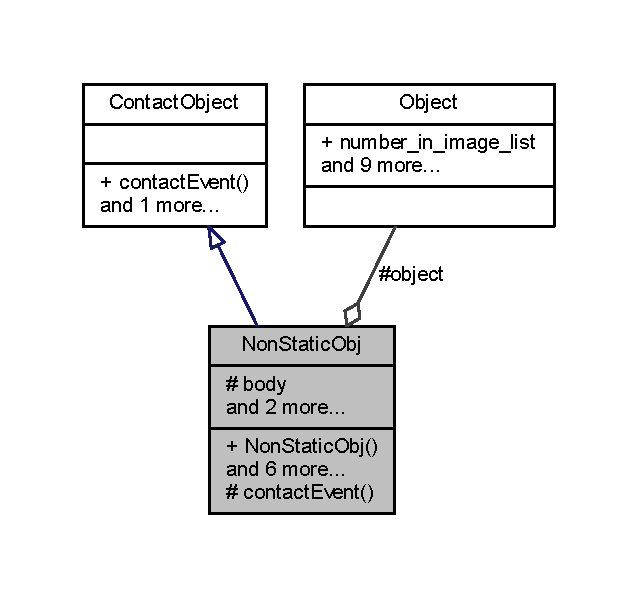
\includegraphics[width=306pt]{class_non_static_obj__coll__graph}
\end{center}
\end{figure}
\subsection*{Public Member Functions}
\begin{DoxyCompactItemize}
\item 
\hyperlink{class_non_static_obj_a0295a381b988a0d0ab17eb3dcc229704}{Non\+Static\+Obj} (b2\+Body $\ast$\+\_\+body, \hyperlink{class_object}{Object} $\ast$\+\_\+object, \hyperlink{_non_static_obj_8h_a842c5e2e69277690b064bf363c017980}{Object\+Type} type)
\begin{DoxyCompactList}\small\item\em Defined constructor for this class. \end{DoxyCompactList}\item 
\hyperlink{_non_static_obj_8h_a842c5e2e69277690b064bf363c017980}{Object\+Type} \hyperlink{class_non_static_obj_a01e6db05d41ec62cb5c258b5069b083e}{who\+AmI} ()
\begin{DoxyCompactList}\small\item\em Allow to define type of an assigned dynamic object. \end{DoxyCompactList}\item 
b2\+Body $\ast$ \hyperlink{class_non_static_obj_a55713a3f848d7629176398333e84a015}{get\+Body} ()
\item 
\hyperlink{class_object}{Object} $\ast$ \hyperlink{class_non_static_obj_abdf0a375a987d99795bd298a1c84940c}{get\+Object} ()
\item 
\mbox{\Hypertarget{class_non_static_obj_a6a67af264af5093665ca91273c9c6f34}\label{class_non_static_obj_a6a67af264af5093665ca91273c9c6f34}} 
virtual void \hyperlink{class_non_static_obj_a6a67af264af5093665ca91273c9c6f34}{update} ()
\begin{DoxyCompactList}\small\item\em update entity state (position in the world, speed etc.) \end{DoxyCompactList}\item 
\mbox{\Hypertarget{class_non_static_obj_a197ed3470e1a7b4f10b1e5567fdc5253}\label{class_non_static_obj_a197ed3470e1a7b4f10b1e5567fdc5253}} 
virtual bool \hyperlink{class_non_static_obj_a197ed3470e1a7b4f10b1e5567fdc5253}{destroy} ()
\begin{DoxyCompactList}\small\item\em destroy the entity \end{DoxyCompactList}\end{DoxyCompactItemize}
\subsection*{Protected Member Functions}
\begin{DoxyCompactItemize}
\item 
\mbox{\Hypertarget{class_non_static_obj_af2a40f79983a88c185c0bf9977e2d50d}\label{class_non_static_obj_af2a40f79983a88c185c0bf9977e2d50d}} 
void \hyperlink{class_non_static_obj_af2a40f79983a88c185c0bf9977e2d50d}{contact\+Event} (b2\+Contact $\ast$contact, bool is\+\_\+begin)
\begin{DoxyCompactList}\small\item\em inherited from \hyperlink{class_contact_object}{Contact\+Object} class \end{DoxyCompactList}\end{DoxyCompactItemize}
\subsection*{Protected Attributes}
\begin{DoxyCompactItemize}
\item 
\mbox{\Hypertarget{class_non_static_obj_a42cf308f091557d0d8a8e6ae8ee0fcf1}\label{class_non_static_obj_a42cf308f091557d0d8a8e6ae8ee0fcf1}} 
b2\+Body $\ast$ \hyperlink{class_non_static_obj_a42cf308f091557d0d8a8e6ae8ee0fcf1}{body}
\begin{DoxyCompactList}\small\item\em pointer to the box2d body assigned to this entity \end{DoxyCompactList}\item 
\mbox{\Hypertarget{class_non_static_obj_a61a8004d502132c7a13258e945300a5e}\label{class_non_static_obj_a61a8004d502132c7a13258e945300a5e}} 
\hyperlink{class_object}{Object} $\ast$ \hyperlink{class_non_static_obj_a61a8004d502132c7a13258e945300a5e}{object}
\begin{DoxyCompactList}\small\item\em pointer to the \hyperlink{class_object}{Object} class assigned to this entity \end{DoxyCompactList}\item 
\mbox{\Hypertarget{class_non_static_obj_a41c92f702f36f05877e74fef1fcb3a71}\label{class_non_static_obj_a41c92f702f36f05877e74fef1fcb3a71}} 
bool \hyperlink{class_non_static_obj_a41c92f702f36f05877e74fef1fcb3a71}{is\+\_\+valid}
\begin{DoxyCompactList}\small\item\em defines the state of the entity \textquotesingle{}true\textquotesingle{} -\/ participate in physics simulation \textquotesingle{}false\textquotesingle{} -\/ doesn\textquotesingle{}t paticipate \end{DoxyCompactList}\item 
\mbox{\Hypertarget{class_non_static_obj_a4328e86d88a94270b88acb0d3965112b}\label{class_non_static_obj_a4328e86d88a94270b88acb0d3965112b}} 
\hyperlink{_non_static_obj_8h_a842c5e2e69277690b064bf363c017980}{Object\+Type} \hyperlink{class_non_static_obj_a4328e86d88a94270b88acb0d3965112b}{my\+\_\+type}
\begin{DoxyCompactList}\small\item\em define type of an dynamic object assigned to this entity \end{DoxyCompactList}\end{DoxyCompactItemize}


\subsection{Detailed Description}
Typical object (an entity) that participates in physics simulation. 

\begin{DoxyAuthor}{Author}
Vasily 
\end{DoxyAuthor}
\begin{DoxyVersion}{Version}
1.\+0 
\end{DoxyVersion}
\begin{DoxyDate}{Date}
June 2017
\end{DoxyDate}
An entity that have only base properties (can\textquotesingle{}t be controlled by the player, fully rely on box2d world rules) 

\subsection{Constructor \& Destructor Documentation}
\mbox{\Hypertarget{class_non_static_obj_a0295a381b988a0d0ab17eb3dcc229704}\label{class_non_static_obj_a0295a381b988a0d0ab17eb3dcc229704}} 
\index{Non\+Static\+Obj@{Non\+Static\+Obj}!Non\+Static\+Obj@{Non\+Static\+Obj}}
\index{Non\+Static\+Obj@{Non\+Static\+Obj}!Non\+Static\+Obj@{Non\+Static\+Obj}}
\subsubsection{\texorpdfstring{Non\+Static\+Obj()}{NonStaticObj()}}
{\footnotesize\ttfamily Non\+Static\+Obj\+::\+Non\+Static\+Obj (\begin{DoxyParamCaption}\item[{b2\+Body $\ast$}]{\+\_\+body,  }\item[{\hyperlink{class_object}{Object} $\ast$}]{\+\_\+object,  }\item[{\hyperlink{_non_static_obj_8h_a842c5e2e69277690b064bf363c017980}{Object\+Type}}]{type }\end{DoxyParamCaption})}



Defined constructor for this class. 


\begin{DoxyParams}{Parameters}
{\em \+\_\+body} & pointer to the box2d body assigned to this entity \\
\hline
{\em \+\_\+object} & pointer to the \hyperlink{class_object}{Object} class assigned to this entity \\
\hline
{\em type} & type from Object\+Type enum of an assigned dynamic object \\
\hline
\end{DoxyParams}


\subsection{Member Function Documentation}
\mbox{\Hypertarget{class_non_static_obj_a55713a3f848d7629176398333e84a015}\label{class_non_static_obj_a55713a3f848d7629176398333e84a015}} 
\index{Non\+Static\+Obj@{Non\+Static\+Obj}!get\+Body@{get\+Body}}
\index{get\+Body@{get\+Body}!Non\+Static\+Obj@{Non\+Static\+Obj}}
\subsubsection{\texorpdfstring{get\+Body()}{getBody()}}
{\footnotesize\ttfamily b2\+Body $\ast$ Non\+Static\+Obj\+::get\+Body (\begin{DoxyParamCaption}{ }\end{DoxyParamCaption})}

\begin{DoxyReturn}{Returns}
pointer to the box2d body assigned to this entity 
\end{DoxyReturn}
\mbox{\Hypertarget{class_non_static_obj_abdf0a375a987d99795bd298a1c84940c}\label{class_non_static_obj_abdf0a375a987d99795bd298a1c84940c}} 
\index{Non\+Static\+Obj@{Non\+Static\+Obj}!get\+Object@{get\+Object}}
\index{get\+Object@{get\+Object}!Non\+Static\+Obj@{Non\+Static\+Obj}}
\subsubsection{\texorpdfstring{get\+Object()}{getObject()}}
{\footnotesize\ttfamily \hyperlink{class_object}{Object} $\ast$ Non\+Static\+Obj\+::get\+Object (\begin{DoxyParamCaption}{ }\end{DoxyParamCaption})}

\begin{DoxyReturn}{Returns}
pointer to the \hyperlink{class_object}{Object} class assigned to this entity 
\end{DoxyReturn}
\mbox{\Hypertarget{class_non_static_obj_a01e6db05d41ec62cb5c258b5069b083e}\label{class_non_static_obj_a01e6db05d41ec62cb5c258b5069b083e}} 
\index{Non\+Static\+Obj@{Non\+Static\+Obj}!who\+AmI@{who\+AmI}}
\index{who\+AmI@{who\+AmI}!Non\+Static\+Obj@{Non\+Static\+Obj}}
\subsubsection{\texorpdfstring{who\+Am\+I()}{whoAmI()}}
{\footnotesize\ttfamily \hyperlink{_non_static_obj_8h_a842c5e2e69277690b064bf363c017980}{Object\+Type} Non\+Static\+Obj\+::who\+AmI (\begin{DoxyParamCaption}{ }\end{DoxyParamCaption})}



Allow to define type of an assigned dynamic object. 

\begin{DoxyReturn}{Returns}
type from Object\+Type enum of an assigned dynamic object 
\end{DoxyReturn}


The documentation for this class was generated from the following files\+:\begin{DoxyCompactItemize}
\item 
\hyperlink{_non_static_obj_8h}{Non\+Static\+Obj.\+h}\item 
Non\+Static\+Obj.\+cpp\end{DoxyCompactItemize}

\hypertarget{class_object}{}\section{Object Class Reference}
\label{class_object}\index{Object@{Object}}


Contains based information about entity which necessary both for \hyperlink{class_model}{Model} and \hyperlink{class_viewer}{Viewer} classes.  




{\ttfamily \#include $<$Level\+Box.\+h$>$}



Collaboration diagram for Object\+:
\nopagebreak
\begin{figure}[H]
\begin{center}
\leavevmode
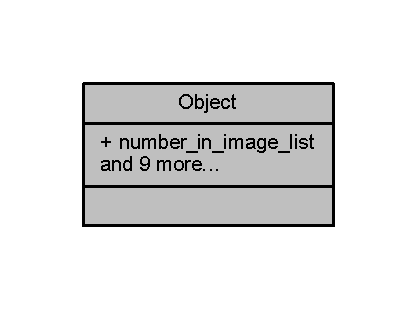
\includegraphics[width=200pt]{class_object__coll__graph}
\end{center}
\end{figure}
\subsection*{Public Attributes}
\begin{DoxyCompactItemize}
\item 
\mbox{\Hypertarget{class_object_a90c94b63236bf5be6946381db72641dc}\label{class_object_a90c94b63236bf5be6946381db72641dc}} 
int \hyperlink{class_object_a90c94b63236bf5be6946381db72641dc}{number\+\_\+in\+\_\+image\+\_\+list}
\begin{DoxyCompactList}\small\item\em number of the images assigned to this entity in the list of all \hyperlink{class_layer}{Layer} images \end{DoxyCompactList}\item 
\mbox{\Hypertarget{class_object_ad3d50969ef24f16edb7337b76a99bb4e}\label{class_object_ad3d50969ef24f16edb7337b76a99bb4e}} 
int \hyperlink{class_object_ad3d50969ef24f16edb7337b76a99bb4e}{top}
\begin{DoxyCompactList}\small\item\em upper coordinate of an image rectangle in whole image (in pixels) \end{DoxyCompactList}\item 
\mbox{\Hypertarget{class_object_a7fc665396287cedde719083c0ec6d28f}\label{class_object_a7fc665396287cedde719083c0ec6d28f}} 
int \hyperlink{class_object_a7fc665396287cedde719083c0ec6d28f}{left}
\begin{DoxyCompactList}\small\item\em left coordinate of an image rectangle in whole image (in pixels) \end{DoxyCompactList}\item 
\mbox{\Hypertarget{class_object_a02010c1708632be33a760486b1f648f8}\label{class_object_a02010c1708632be33a760486b1f648f8}} 
double \hyperlink{class_object_a02010c1708632be33a760486b1f648f8}{x}
\begin{DoxyCompactList}\small\item\em x coordinate of an object relatively \hyperlink{class_layer}{Layer} (in pixels) \end{DoxyCompactList}\item 
\mbox{\Hypertarget{class_object_a542c4d6094ace575fb4a28f46b9cc6a1}\label{class_object_a542c4d6094ace575fb4a28f46b9cc6a1}} 
double \hyperlink{class_object_a542c4d6094ace575fb4a28f46b9cc6a1}{y}
\begin{DoxyCompactList}\small\item\em y coordinate of an object relatively \hyperlink{class_layer}{Layer} (in pixels) \end{DoxyCompactList}\item 
\mbox{\Hypertarget{class_object_a811bf2cbf614c4f0a3935a83fb639ffd}\label{class_object_a811bf2cbf614c4f0a3935a83fb639ffd}} 
double \hyperlink{class_object_a811bf2cbf614c4f0a3935a83fb639ffd}{height}
\begin{DoxyCompactList}\small\item\em height of an object (in pixels) \end{DoxyCompactList}\item 
\mbox{\Hypertarget{class_object_a3afad0ab476968e517b6f48c2a32719f}\label{class_object_a3afad0ab476968e517b6f48c2a32719f}} 
double \hyperlink{class_object_a3afad0ab476968e517b6f48c2a32719f}{width}
\begin{DoxyCompactList}\small\item\em width of an object (in pixels) \end{DoxyCompactList}\item 
\mbox{\Hypertarget{class_object_afb2fc6bd0f2d6e62901f6b68ac7dfbc8}\label{class_object_afb2fc6bd0f2d6e62901f6b68ac7dfbc8}} 
double \hyperlink{class_object_afb2fc6bd0f2d6e62901f6b68ac7dfbc8}{rotation}
\begin{DoxyCompactList}\small\item\em rotate angle of an object (in radians) \end{DoxyCompactList}\item 
\mbox{\Hypertarget{class_object_ae0881e8e5fd72a025663b048f2444555}\label{class_object_ae0881e8e5fd72a025663b048f2444555}} 
bool \hyperlink{class_object_ae0881e8e5fd72a025663b048f2444555}{is\+\_\+valid}
\begin{DoxyCompactList}\small\item\em state of an object\+: \textquotesingle{}true\textquotesingle{} -\/ have to be dispalyed; \textquotesingle{}false\textquotesingle{} -\/ doesnt\textquotesingle{}t have to \end{DoxyCompactList}\item 
\mbox{\Hypertarget{class_object_aff7027899040a66fc27b9c059f9c13f0}\label{class_object_aff7027899040a66fc27b9c059f9c13f0}} 
int \hyperlink{class_object_aff7027899040a66fc27b9c059f9c13f0}{transparensy}
\begin{DoxyCompactList}\small\item\em degree of transparensy (0-\/fully transperent; 255-\/fully opaque) \end{DoxyCompactList}\end{DoxyCompactItemize}


\subsection{Detailed Description}
Contains based information about entity which necessary both for \hyperlink{class_model}{Model} and \hyperlink{class_viewer}{Viewer} classes. 

\begin{DoxyAuthor}{Author}
Vasily 
\end{DoxyAuthor}
\begin{DoxyVersion}{Version}
1.\+0 
\end{DoxyVersion}
\begin{DoxyDate}{Date}
June 2017 
\end{DoxyDate}


The documentation for this class was generated from the following file\+:\begin{DoxyCompactItemize}
\item 
\hyperlink{_level_box_8h}{Level\+Box.\+h}\end{DoxyCompactItemize}

\hypertarget{class_platform}{}\section{Platform Class Reference}
\label{class_platform}\index{Platform@{Platform}}


Kinematic object moving along the trajectory.  




{\ttfamily \#include $<$Platform.\+h$>$}



Collaboration diagram for Platform\+:
\nopagebreak
\begin{figure}[H]
\begin{center}
\leavevmode
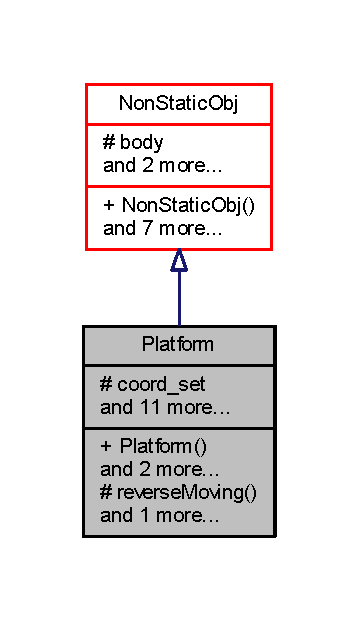
\includegraphics[width=294pt]{class_platform__coll__graph}
\end{center}
\end{figure}
\subsection*{Public Member Functions}
\begin{DoxyCompactItemize}
\item 
\hyperlink{class_platform_a7c8e5045e5df1165c1154605e1a05339}{Platform} (int \+\_\+level\+\_\+width, int \+\_\+level\+\_\+height, b2\+Body $\ast$\+\_\+body, \hyperlink{class_object}{Object} $\ast$\+\_\+object, std\+::vector$<$ std\+::pair$<$ double, double $>$$>$ \+\_\+traj\+\_\+coord, int \+\_\+fixed\+\_\+speed, bool \+\_\+is\+\_\+rounded, int \+\_\+node\+\_\+number)
\begin{DoxyCompactList}\small\item\em Defined constructor for this class. \end{DoxyCompactList}\item 
\mbox{\Hypertarget{class_platform_aa601f00a3625669bb39252cfc932efa0}\label{class_platform_aa601f00a3625669bb39252cfc932efa0}} 
void \hyperlink{class_platform_aa601f00a3625669bb39252cfc932efa0}{update} ()
\begin{DoxyCompactList}\small\item\em inherited from \hyperlink{class_non_static_obj}{Non\+Static\+Obj} class \end{DoxyCompactList}\end{DoxyCompactItemize}
\subsection*{Protected Member Functions}
\begin{DoxyCompactItemize}
\item 
\mbox{\Hypertarget{class_platform_aae68e047eaa1046773ad62654c99421a}\label{class_platform_aae68e047eaa1046773ad62654c99421a}} 
void \hyperlink{class_platform_aae68e047eaa1046773ad62654c99421a}{reverse\+Moving} ()
\begin{DoxyCompactList}\small\item\em causes platform to begin reverse moving \end{DoxyCompactList}\item 
\mbox{\Hypertarget{class_platform_a5462c5ec9fc865988ffccd2e0d67b2a9}\label{class_platform_a5462c5ec9fc865988ffccd2e0d67b2a9}} 
void \hyperlink{class_platform_a5462c5ec9fc865988ffccd2e0d67b2a9}{to\+Next\+Point} ()
\begin{DoxyCompactList}\small\item\em causes platform to begin moving to the next point \end{DoxyCompactList}\end{DoxyCompactItemize}
\subsection*{Protected Attributes}
\begin{DoxyCompactItemize}
\item 
\mbox{\Hypertarget{class_platform_a17b9655a30c0c75e237cb54ce5939901}\label{class_platform_a17b9655a30c0c75e237cb54ce5939901}} 
std\+::vector$<$ std\+::pair$<$ double, double $>$ $>$ \hyperlink{class_platform_a17b9655a30c0c75e237cb54ce5939901}{coord\+\_\+set}
\begin{DoxyCompactList}\small\item\em set of the trajectory coordinates for this platform \end{DoxyCompactList}\item 
\mbox{\Hypertarget{class_platform_a5cffd298e38b51b6a079721d9ddafd1a}\label{class_platform_a5cffd298e38b51b6a079721d9ddafd1a}} 
int \hyperlink{class_platform_a5cffd298e38b51b6a079721d9ddafd1a}{point\+\_\+iter}
\begin{DoxyCompactList}\small\item\em current node of the trajectory for this platform \end{DoxyCompactList}\item 
\mbox{\Hypertarget{class_platform_a6a72a0e87078f6ec39d2638b0826c3f9}\label{class_platform_a6a72a0e87078f6ec39d2638b0826c3f9}} 
int \hyperlink{class_platform_a6a72a0e87078f6ec39d2638b0826c3f9}{incr}
\begin{DoxyCompactList}\small\item\em current increment or decrement of point\+\_\+iter \end{DoxyCompactList}\item 
\mbox{\Hypertarget{class_platform_ac7e442d3f0cbb881046089a27de27270}\label{class_platform_ac7e442d3f0cbb881046089a27de27270}} 
int \hyperlink{class_platform_ac7e442d3f0cbb881046089a27de27270}{node\+\_\+number}
\begin{DoxyCompactList}\small\item\em max number of trajectory nodes which platform passed before reverse moving or the stop \end{DoxyCompactList}\item 
\mbox{\Hypertarget{class_platform_ac237ae97ec177455984a8ceb80ad294a}\label{class_platform_ac237ae97ec177455984a8ceb80ad294a}} 
int \hyperlink{class_platform_ac237ae97ec177455984a8ceb80ad294a}{counter}
\begin{DoxyCompactList}\small\item\em the number of passed nodes \end{DoxyCompactList}\item 
\mbox{\Hypertarget{class_platform_a36158e28df3d35b04ffa531cde921e48}\label{class_platform_a36158e28df3d35b04ffa531cde921e48}} 
int \hyperlink{class_platform_a36158e28df3d35b04ffa531cde921e48}{counter\+\_\+incr}
\begin{DoxyCompactList}\small\item\em current increment or decrement of counter \end{DoxyCompactList}\item 
\mbox{\Hypertarget{class_platform_a03da0eb526cdf8ae29cdc626b07fcf3e}\label{class_platform_a03da0eb526cdf8ae29cdc626b07fcf3e}} 
int \hyperlink{class_platform_a03da0eb526cdf8ae29cdc626b07fcf3e}{fixed\+\_\+speed}
\begin{DoxyCompactList}\small\item\em speed of the platform \end{DoxyCompactList}\item 
\mbox{\Hypertarget{class_platform_ac9eacf4c7c58d649be944b94ffeeb7b5}\label{class_platform_ac9eacf4c7c58d649be944b94ffeeb7b5}} 
int \hyperlink{class_platform_ac9eacf4c7c58d649be944b94ffeeb7b5}{level\+\_\+width}
\begin{DoxyCompactList}\small\item\em width of the current level \end{DoxyCompactList}\item 
\mbox{\Hypertarget{class_platform_a180664b41270365d3be526b48fa2567b}\label{class_platform_a180664b41270365d3be526b48fa2567b}} 
int \hyperlink{class_platform_a180664b41270365d3be526b48fa2567b}{level\+\_\+height}
\begin{DoxyCompactList}\small\item\em height of the current level \end{DoxyCompactList}\item 
\mbox{\Hypertarget{class_platform_ab3e380bb3ba10bb3ab5c58e0d37f9095}\label{class_platform_ab3e380bb3ba10bb3ab5c58e0d37f9095}} 
bool \hyperlink{class_platform_ab3e380bb3ba10bb3ab5c58e0d37f9095}{is\+\_\+rouded}
\begin{DoxyCompactList}\small\item\em defines the shape of trajectory \textquotesingle{}true\textquotesingle{} -\/ closed \textquotesingle{}false\textquotesingle{} -\/ torn \end{DoxyCompactList}\item 
\mbox{\Hypertarget{class_platform_a3a9d45f38361924cb60ef5b17bef0cac}\label{class_platform_a3a9d45f38361924cb60ef5b17bef0cac}} 
bool \hyperlink{class_platform_a3a9d45f38361924cb60ef5b17bef0cac}{is\+\_\+active}
\begin{DoxyCompactList}\small\item\em defines the state of the platform \textquotesingle{}true\textquotesingle{} -\/ moves \textquotesingle{}false\textquotesingle{} -\/ doesn\textquotesingle{}t move \end{DoxyCompactList}\item 
\mbox{\Hypertarget{class_platform_a2f120cbb66ac4972fdd05ba816484dc0}\label{class_platform_a2f120cbb66ac4972fdd05ba816484dc0}} 
b2\+Vec2 \hyperlink{class_platform_a2f120cbb66ac4972fdd05ba816484dc0}{tmp}
\begin{DoxyCompactList}\small\item\em temprorary storage for platform coordinates \end{DoxyCompactList}\end{DoxyCompactItemize}


\subsection{Detailed Description}
Kinematic object moving along the trajectory. 

\begin{DoxyAuthor}{Author}
Vasily 
\end{DoxyAuthor}
\begin{DoxyVersion}{Version}
1.\+0 
\end{DoxyVersion}
\begin{DoxyDate}{Date}
June 2017 
\end{DoxyDate}


\subsection{Constructor \& Destructor Documentation}
\mbox{\Hypertarget{class_platform_a7c8e5045e5df1165c1154605e1a05339}\label{class_platform_a7c8e5045e5df1165c1154605e1a05339}} 
\index{Platform@{Platform}!Platform@{Platform}}
\index{Platform@{Platform}!Platform@{Platform}}
\subsubsection{\texorpdfstring{Platform()}{Platform()}}
{\footnotesize\ttfamily Platform\+::\+Platform (\begin{DoxyParamCaption}\item[{int}]{\+\_\+level\+\_\+width,  }\item[{int}]{\+\_\+level\+\_\+height,  }\item[{b2\+Body $\ast$}]{\+\_\+body,  }\item[{\hyperlink{class_object}{Object} $\ast$}]{\+\_\+object,  }\item[{std\+::vector$<$ std\+::pair$<$ double, double $>$$>$}]{\+\_\+traj\+\_\+coord,  }\item[{int}]{\+\_\+fixed\+\_\+speed,  }\item[{bool}]{\+\_\+is\+\_\+rounded,  }\item[{int}]{\+\_\+node\+\_\+number }\end{DoxyParamCaption})}



Defined constructor for this class. 


\begin{DoxyParams}{Parameters}
{\em \+\_\+level\+\_\+width} & the width in pixels of this level \\
\hline
{\em \+\_\+level\+\_\+height} & the height in pixels of this level \\
\hline
{\em \+\_\+body} & pointer to the box2d body assigned to this platform \\
\hline
{\em \+\_\+object} & pointer to the \hyperlink{class_object}{Object} class assigned to this platform \\
\hline
{\em \+\_\+traj\+\_\+coord} & set of the trajectory coordinates for this platform \\
\hline
{\em \+\_\+fixed\+\_\+speed} & speed of the platform \\
\hline
{\em \+\_\+is\+\_\+rounded} & defines the shape of trajectory \textquotesingle{}true\textquotesingle{} -\/ closed \textquotesingle{}false\textquotesingle{} -\/ torn \\
\hline
{\em \+\_\+node\+\_\+number} & max number of trajectory nodes which platform passed before reverse moving or the stop \\
\hline
\end{DoxyParams}


The documentation for this class was generated from the following files\+:\begin{DoxyCompactItemize}
\item 
\hyperlink{_platform_8h}{Platform.\+h}\item 
Platform.\+cpp\end{DoxyCompactItemize}

\hypertarget{class_player}{}\section{Player Class Reference}
\label{class_player}\index{Player@{Player}}


Parent class for \hyperlink{class_dexterous_player}{Dexterous\+Player} and \hyperlink{class_strong_player}{Strong\+Player} classes.  




{\ttfamily \#include $<$Player.\+h$>$}



Collaboration diagram for Player\+:\nopagebreak
\begin{figure}[H]
\begin{center}
\leavevmode
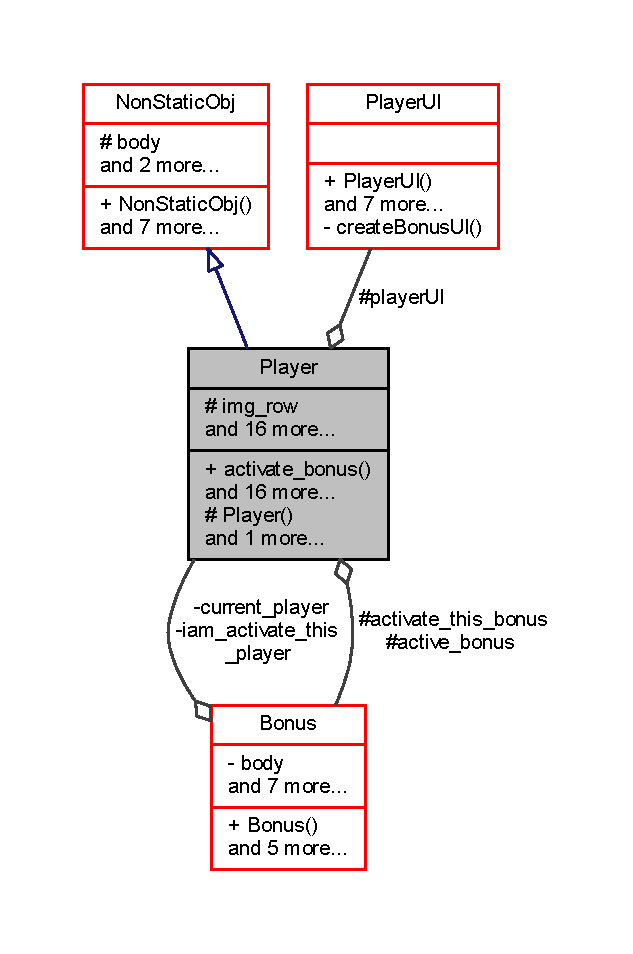
\includegraphics[width=304pt]{class_player__coll__graph}
\end{center}
\end{figure}
\subsection*{Public Member Functions}
\begin{DoxyCompactItemize}
\item 
void \hyperlink{class_player_a18c12a3d320a15d87539cd6de2acca66}{activate\+\_\+bonus} (double modificator, Bonus\+Type bonus\+\_\+type)
\begin{DoxyCompactList}\small\item\em Apllies the bonus effect to the hero. \end{DoxyCompactList}\item 
void \hyperlink{class_player_a984c3a87de751efe818203bb01e8d5e9}{deactivate\+\_\+bonus} (double modificator, Bonus\+Type bonus\+\_\+type)
\begin{DoxyCompactList}\small\item\em Terminates the action of the bonus effect to the hero. \end{DoxyCompactList}\item 
\mbox{\Hypertarget{class_player_a70e21ca98281b7d72f105f2693113d7e}\label{class_player_a70e21ca98281b7d72f105f2693113d7e}} 
void \hyperlink{class_player_a70e21ca98281b7d72f105f2693113d7e}{jump} ()
\begin{DoxyCompactList}\small\item\em causes the hero to jump \end{DoxyCompactList}\item 
\mbox{\Hypertarget{class_player_ae3bbcf1159bdc059bff1c2513f2505f7}\label{class_player_ae3bbcf1159bdc059bff1c2513f2505f7}} 
void \hyperlink{class_player_ae3bbcf1159bdc059bff1c2513f2505f7}{move\+Left} ()
\begin{DoxyCompactList}\small\item\em causes the hero to increase left-\/moving speed \end{DoxyCompactList}\item 
\mbox{\Hypertarget{class_player_a6a2b68bc4b21d4c4a79a23b498896ec2}\label{class_player_a6a2b68bc4b21d4c4a79a23b498896ec2}} 
void \hyperlink{class_player_a6a2b68bc4b21d4c4a79a23b498896ec2}{move\+Right} ()
\begin{DoxyCompactList}\small\item\em causes the hero to increase right-\/moving speed \end{DoxyCompactList}\item 
\mbox{\Hypertarget{class_player_afebb6b7ca7210e7b1aa2c9ee4ff75b0e}\label{class_player_afebb6b7ca7210e7b1aa2c9ee4ff75b0e}} 
void \hyperlink{class_player_afebb6b7ca7210e7b1aa2c9ee4ff75b0e}{stop\+Right} ()
\begin{DoxyCompactList}\small\item\em causes the hero to decrease right-\/moving speed \end{DoxyCompactList}\item 
\mbox{\Hypertarget{class_player_aa150f941486096bb63cc67eabec9046c}\label{class_player_aa150f941486096bb63cc67eabec9046c}} 
void \hyperlink{class_player_aa150f941486096bb63cc67eabec9046c}{stop\+Left} ()
\begin{DoxyCompactList}\small\item\em causes the hero to decrease left-\/moving speed \end{DoxyCompactList}\item 
\mbox{\Hypertarget{class_player_aaefa871e86a0ae126f3654b1078e0ffa}\label{class_player_aaefa871e86a0ae126f3654b1078e0ffa}} 
void \hyperlink{class_player_aaefa871e86a0ae126f3654b1078e0ffa}{just\+Stop} ()
\begin{DoxyCompactList}\small\item\em causes the hero to stop completely \end{DoxyCompactList}\item 
double \hyperlink{class_player_afbabae83ae2b21caf794efa91e26c37d}{get\+Vel} ()
\item 
void \hyperlink{class_player_ade0e4463e66975e549986ce55cac9467}{set\+Vel} (double des\+\_\+vel)
\item 
\mbox{\Hypertarget{class_player_a35883d3f8b0087209e9f5989fd4142db}\label{class_player_a35883d3f8b0087209e9f5989fd4142db}} 
void \hyperlink{class_player_a35883d3f8b0087209e9f5989fd4142db}{begin\+Contact\+With\+Ground} ()
\begin{DoxyCompactList}\small\item\em Notifies about the begginning of the hero\textquotesingle{}s contact with the ground. \end{DoxyCompactList}\item 
\mbox{\Hypertarget{class_player_aadd86e4d822fb07db4a37856506d16e7}\label{class_player_aadd86e4d822fb07db4a37856506d16e7}} 
void \hyperlink{class_player_aadd86e4d822fb07db4a37856506d16e7}{end\+Contact\+With\+Ground} ()
\begin{DoxyCompactList}\small\item\em Notifies about the end of the hero\textquotesingle{}s contact with the ground. \end{DoxyCompactList}\item 
\hyperlink{class_bonus}{Bonus} $\ast$$\ast$ \hyperlink{class_player_ab62b84f866fb3075bfbf8ea455d73375}{get\+Activation\+Bonus} ()
\item 
void \hyperlink{class_player_ab3d8dc6872a9903ea2717b57d77790a3}{return\+Coordinates} (double $\ast$x, double $\ast$y)
\item 
\hyperlink{class_player_u_i}{Player\+UI} $\ast$ \hyperlink{class_player_aefa23e8642f25b0f7e72543599d567f6}{return\+UI} ()
\item 
\mbox{\Hypertarget{class_player_ad4d4b9138657ce9cde8433a44b1c4225}\label{class_player_ad4d4b9138657ce9cde8433a44b1c4225}} 
bool \hyperlink{class_player_ad4d4b9138657ce9cde8433a44b1c4225}{destroy} ()
\begin{DoxyCompactList}\small\item\em destroy the hero \end{DoxyCompactList}\item 
\mbox{\Hypertarget{class_player_a82c3476f3e65a4e2ac6bcd040771bdd4}\label{class_player_a82c3476f3e65a4e2ac6bcd040771bdd4}} 
void \hyperlink{class_player_a82c3476f3e65a4e2ac6bcd040771bdd4}{update} ()
\begin{DoxyCompactList}\small\item\em inherited from \hyperlink{class_non_static_obj}{Non\+Static\+Obj} class \end{DoxyCompactList}\end{DoxyCompactItemize}
\subsection*{Protected Member Functions}
\begin{DoxyCompactItemize}
\item 
\hyperlink{class_player_abf1330c477ecd5d2c0154a4876cf4154}{Player} (int \+\_\+level\+\_\+width, int \+\_\+level\+\_\+height, b2\+Body $\ast$\+\_\+body, \hyperlink{class_object}{Object} $\ast$\+\_\+object, int \+\_\+health, Return\+Events $\ast$\+\_\+re)
\begin{DoxyCompactList}\small\item\em Defined constructor for this class. \end{DoxyCompactList}\item 
\mbox{\Hypertarget{class_player_add3d6c730bb80c4d3a125e41d5586007}\label{class_player_add3d6c730bb80c4d3a125e41d5586007}} 
void \hyperlink{class_player_add3d6c730bb80c4d3a125e41d5586007}{update\+UI} ()
\begin{DoxyCompactList}\small\item\em Update UI information for this hero. \end{DoxyCompactList}\end{DoxyCompactItemize}
\subsection*{Protected Attributes}
\begin{DoxyCompactItemize}
\item 
\mbox{\Hypertarget{class_player_a07824bd51e3fb726f481c1e5f3e695a6}\label{class_player_a07824bd51e3fb726f481c1e5f3e695a6}} 
int \hyperlink{class_player_a07824bd51e3fb726f481c1e5f3e695a6}{img\+\_\+row}
\begin{DoxyCompactList}\small\item\em current row in image tileset for this hero \end{DoxyCompactList}\item 
\mbox{\Hypertarget{class_player_a336d4b7a8eb04bcffcfe62a69f8bff52}\label{class_player_a336d4b7a8eb04bcffcfe62a69f8bff52}} 
int \hyperlink{class_player_a336d4b7a8eb04bcffcfe62a69f8bff52}{left\+\_\+row}
\begin{DoxyCompactList}\small\item\em row in image tileset for left moving \end{DoxyCompactList}\item 
\mbox{\Hypertarget{class_player_a68fd86a5c42d0619eff999228b0be898}\label{class_player_a68fd86a5c42d0619eff999228b0be898}} 
int \hyperlink{class_player_a68fd86a5c42d0619eff999228b0be898}{right\+\_\+row}
\begin{DoxyCompactList}\small\item\em row in image tileset for right moving \end{DoxyCompactList}\item 
\mbox{\Hypertarget{class_player_a2eee5f54a0b42e1a98045ddbe25a75ca}\label{class_player_a2eee5f54a0b42e1a98045ddbe25a75ca}} 
int \hyperlink{class_player_a2eee5f54a0b42e1a98045ddbe25a75ca}{max\+\_\+frame}
\begin{DoxyCompactList}\small\item\em max column number in image tileset \end{DoxyCompactList}\item 
\mbox{\Hypertarget{class_player_a879ea860c2b4f99dada44ae8672aeeb1}\label{class_player_a879ea860c2b4f99dada44ae8672aeeb1}} 
int \hyperlink{class_player_a879ea860c2b4f99dada44ae8672aeeb1}{fixed\+\_\+speed}
\begin{DoxyCompactList}\small\item\em default speed of the character \end{DoxyCompactList}\item 
\mbox{\Hypertarget{class_player_a5a61bfa96e90f3fbf5d89efc0872915f}\label{class_player_a5a61bfa96e90f3fbf5d89efc0872915f}} 
int \hyperlink{class_player_a5a61bfa96e90f3fbf5d89efc0872915f}{level\+\_\+width}
\begin{DoxyCompactList}\small\item\em width of the current level \end{DoxyCompactList}\item 
\mbox{\Hypertarget{class_player_a5543a988cb2e91cf2e61b60ff5382ce9}\label{class_player_a5543a988cb2e91cf2e61b60ff5382ce9}} 
int \hyperlink{class_player_a5543a988cb2e91cf2e61b60ff5382ce9}{level\+\_\+height}
\begin{DoxyCompactList}\small\item\em height of the current level \end{DoxyCompactList}\item 
\mbox{\Hypertarget{class_player_ad38061042ee0864383dab6935fa0acea}\label{class_player_ad38061042ee0864383dab6935fa0acea}} 
int \hyperlink{class_player_ad38061042ee0864383dab6935fa0acea}{max\+\_\+health}
\begin{DoxyCompactList}\small\item\em the maximum level of health reserve for this caracter \end{DoxyCompactList}\item 
\mbox{\Hypertarget{class_player_aad33b52bfe73c4c978a3135172f286a0}\label{class_player_aad33b52bfe73c4c978a3135172f286a0}} 
int \hyperlink{class_player_aad33b52bfe73c4c978a3135172f286a0}{health}
\begin{DoxyCompactList}\small\item\em current level of health reserve for this caracter \end{DoxyCompactList}\item 
\mbox{\Hypertarget{class_player_a2dc679f61d4728895221afb567aede2f}\label{class_player_a2dc679f61d4728895221afb567aede2f}} 
int \hyperlink{class_player_a2dc679f61d4728895221afb567aede2f}{on\+\_\+ground}
\begin{DoxyCompactList}\small\item\em Define character position \textquotesingle{}false\textquotesingle{} -\/ in air; \textquotesingle{}true\textquotesingle{} -\/ on ground. \end{DoxyCompactList}\item 
\mbox{\Hypertarget{class_player_a9f581a28a4ffac4120411abb6d8ffb34}\label{class_player_a9f581a28a4ffac4120411abb6d8ffb34}} 
bool \hyperlink{class_player_a9f581a28a4ffac4120411abb6d8ffb34}{is\+\_\+animated}
\begin{DoxyCompactList}\small\item\em Define characters animation \textquotesingle{}false\textquotesingle{} -\/ non-\/animated; \textquotesingle{}true\textquotesingle{} -\/ animated. \end{DoxyCompactList}\item 
\mbox{\Hypertarget{class_player_a943966c052b8bfc40439248a2d4e3f8f}\label{class_player_a943966c052b8bfc40439248a2d4e3f8f}} 
double \hyperlink{class_player_a943966c052b8bfc40439248a2d4e3f8f}{current\+\_\+frame}
\begin{DoxyCompactList}\small\item\em current column number in image tileset \end{DoxyCompactList}\item 
\mbox{\Hypertarget{class_player_ad469c1133f407b68e90d587013b20c71}\label{class_player_ad469c1133f407b68e90d587013b20c71}} 
double \hyperlink{class_player_ad469c1133f407b68e90d587013b20c71}{current\+\_\+frequency}
\begin{DoxyCompactList}\small\item\em speed of hero animation \end{DoxyCompactList}\item 
\mbox{\Hypertarget{class_player_a8a96a60e7820f887bc0ff8e15aaf5639}\label{class_player_a8a96a60e7820f887bc0ff8e15aaf5639}} 
double \hyperlink{class_player_a8a96a60e7820f887bc0ff8e15aaf5639}{x\+\_\+speed}
\begin{DoxyCompactList}\small\item\em current speed of the hero \end{DoxyCompactList}\item 
\mbox{\Hypertarget{class_player_a7798d4f62911339f255225b9f59ae497}\label{class_player_a7798d4f62911339f255225b9f59ae497}} 
double \hyperlink{class_player_a7798d4f62911339f255225b9f59ae497}{desired\+\_\+vel}
\begin{DoxyCompactList}\small\item\em delta-\/speed for maintaining constant speed in physics world \end{DoxyCompactList}\item 
\mbox{\Hypertarget{class_player_aadeca24363f2fb5d9206a2cf9c552c20}\label{class_player_aadeca24363f2fb5d9206a2cf9c552c20}} 
double \hyperlink{class_player_aadeca24363f2fb5d9206a2cf9c552c20}{jump\+\_\+strenght}
\begin{DoxyCompactList}\small\item\em strenght of the heros jump \end{DoxyCompactList}\item 
\mbox{\Hypertarget{class_player_a652a51b511e40c14cd43c906693670f6}\label{class_player_a652a51b511e40c14cd43c906693670f6}} 
Return\+Events $\ast$ \hyperlink{class_player_a652a51b511e40c14cd43c906693670f6}{re}
\begin{DoxyCompactList}\small\item\em pointer to the variable, which contains reply of the current level during last iteration (see \hyperlink{class_layer}{Layer} class) \end{DoxyCompactList}\item 
\mbox{\Hypertarget{class_player_ac1b10a27f5fac807cd2a2ff00018b18d}\label{class_player_ac1b10a27f5fac807cd2a2ff00018b18d}} 
\hyperlink{class_bonus}{Bonus} $\ast$ \hyperlink{class_player_ac1b10a27f5fac807cd2a2ff00018b18d}{activate\+\_\+this\+\_\+bonus}
\begin{DoxyCompactList}\small\item\em Pointer to the bonus which will be activated at the next update iteration. \end{DoxyCompactList}\item 
\mbox{\Hypertarget{class_player_aa9320da45054e6196476c46b9b0ac794}\label{class_player_aa9320da45054e6196476c46b9b0ac794}} 
\hyperlink{class_bonus}{Bonus} $\ast$ \hyperlink{class_player_aa9320da45054e6196476c46b9b0ac794}{active\+\_\+bonus} \mbox{[}3\mbox{]}
\begin{DoxyCompactList}\small\item\em Pointer to the array of player ui bonus cell. \end{DoxyCompactList}\item 
\mbox{\Hypertarget{class_player_a31637dcf493a77b73258e87641b339d4}\label{class_player_a31637dcf493a77b73258e87641b339d4}} 
\hyperlink{class_player_u_i}{Player\+UI} {\bfseries player\+UI}
\end{DoxyCompactItemize}


\subsection{Detailed Description}
Parent class for \hyperlink{class_dexterous_player}{Dexterous\+Player} and \hyperlink{class_strong_player}{Strong\+Player} classes. 

\begin{DoxyAuthor}{Author}
Vasily 
\end{DoxyAuthor}
\begin{DoxyVersion}{Version}
1.\+0 
\end{DoxyVersion}
\begin{DoxyDate}{Date}
June 2017
\end{DoxyDate}
Contain base information about characret besides its type 

\subsection{Constructor \& Destructor Documentation}
\mbox{\Hypertarget{class_player_abf1330c477ecd5d2c0154a4876cf4154}\label{class_player_abf1330c477ecd5d2c0154a4876cf4154}} 
\index{Player@{Player}!Player@{Player}}
\index{Player@{Player}!Player@{Player}}
\subsubsection{\texorpdfstring{Player()}{Player()}}
{\footnotesize\ttfamily Player\+::\+Player (\begin{DoxyParamCaption}\item[{int}]{\+\_\+level\+\_\+width,  }\item[{int}]{\+\_\+level\+\_\+height,  }\item[{b2\+Body $\ast$}]{\+\_\+body,  }\item[{\hyperlink{class_object}{Object} $\ast$}]{\+\_\+object,  }\item[{int}]{\+\_\+health,  }\item[{Return\+Events $\ast$}]{\+\_\+re }\end{DoxyParamCaption})\hspace{0.3cm}{\ttfamily [protected]}}



Defined constructor for this class. 


\begin{DoxyParams}{Parameters}
{\em \+\_\+level\+\_\+width} & the width in pixels of this level \\
\hline
{\em \+\_\+level\+\_\+height} & the height in pixels of this level \\
\hline
{\em \+\_\+body} & pointer to the box2d body assigned to this character \\
\hline
{\em \+\_\+object} & pointer to the \hyperlink{class_object}{Object} class assigned to this character \\
\hline
{\em \+\_\+health} & the maximum level of health reserve for this caracter \\
\hline
{\em \+\_\+re} & pointer to the variable which contains reply of the current level during last iteration (see \hyperlink{class_layer}{Layer} class) \\
\hline
\end{DoxyParams}


\subsection{Member Function Documentation}
\mbox{\Hypertarget{class_player_a18c12a3d320a15d87539cd6de2acca66}\label{class_player_a18c12a3d320a15d87539cd6de2acca66}} 
\index{Player@{Player}!activate\+\_\+bonus@{activate\+\_\+bonus}}
\index{activate\+\_\+bonus@{activate\+\_\+bonus}!Player@{Player}}
\subsubsection{\texorpdfstring{activate\+\_\+bonus()}{activate\_bonus()}}
{\footnotesize\ttfamily void Player\+::activate\+\_\+bonus (\begin{DoxyParamCaption}\item[{double}]{modificator,  }\item[{Bonus\+Type}]{bonus\+\_\+type }\end{DoxyParamCaption})}



Apllies the bonus effect to the hero. 


\begin{DoxyParams}{Parameters}
{\em modificator} & bonuse strength of impact \\
\hline
{\em bonus\+\_\+type} & bonuse type (see enum Bonus\+Type) \\
\hline
\end{DoxyParams}
\mbox{\Hypertarget{class_player_a984c3a87de751efe818203bb01e8d5e9}\label{class_player_a984c3a87de751efe818203bb01e8d5e9}} 
\index{Player@{Player}!deactivate\+\_\+bonus@{deactivate\+\_\+bonus}}
\index{deactivate\+\_\+bonus@{deactivate\+\_\+bonus}!Player@{Player}}
\subsubsection{\texorpdfstring{deactivate\+\_\+bonus()}{deactivate\_bonus()}}
{\footnotesize\ttfamily void Player\+::deactivate\+\_\+bonus (\begin{DoxyParamCaption}\item[{double}]{modificator,  }\item[{Bonus\+Type}]{bonus\+\_\+type }\end{DoxyParamCaption})}



Terminates the action of the bonus effect to the hero. 


\begin{DoxyParams}{Parameters}
{\em modificator} & bonuse strength of impact \\
\hline
{\em bonus\+\_\+type} & bonuse type (see enum Bonus\+Type) \\
\hline
\end{DoxyParams}
\mbox{\Hypertarget{class_player_ab62b84f866fb3075bfbf8ea455d73375}\label{class_player_ab62b84f866fb3075bfbf8ea455d73375}} 
\index{Player@{Player}!get\+Activation\+Bonus@{get\+Activation\+Bonus}}
\index{get\+Activation\+Bonus@{get\+Activation\+Bonus}!Player@{Player}}
\subsubsection{\texorpdfstring{get\+Activation\+Bonus()}{getActivationBonus()}}
{\footnotesize\ttfamily \hyperlink{class_bonus}{Bonus} $\ast$$\ast$ Player\+::get\+Activation\+Bonus (\begin{DoxyParamCaption}{ }\end{DoxyParamCaption})}

\begin{DoxyReturn}{Returns}
pointer to the bonus which will be activated at the next update iteration 
\end{DoxyReturn}
\mbox{\Hypertarget{class_player_afbabae83ae2b21caf794efa91e26c37d}\label{class_player_afbabae83ae2b21caf794efa91e26c37d}} 
\index{Player@{Player}!get\+Vel@{get\+Vel}}
\index{get\+Vel@{get\+Vel}!Player@{Player}}
\subsubsection{\texorpdfstring{get\+Vel()}{getVel()}}
{\footnotesize\ttfamily double Player\+::get\+Vel (\begin{DoxyParamCaption}{ }\end{DoxyParamCaption})}

\begin{DoxyReturn}{Returns}
current hero speed 
\end{DoxyReturn}
\mbox{\Hypertarget{class_player_ab3d8dc6872a9903ea2717b57d77790a3}\label{class_player_ab3d8dc6872a9903ea2717b57d77790a3}} 
\index{Player@{Player}!return\+Coordinates@{return\+Coordinates}}
\index{return\+Coordinates@{return\+Coordinates}!Player@{Player}}
\subsubsection{\texorpdfstring{return\+Coordinates()}{returnCoordinates()}}
{\footnotesize\ttfamily void Player\+::return\+Coordinates (\begin{DoxyParamCaption}\item[{double $\ast$}]{x,  }\item[{double $\ast$}]{y }\end{DoxyParamCaption})}

Set in input arguments current hero coordinates 
\begin{DoxyParams}{Parameters}
{\em x} & pointer to the variable where set x coordinate \\
\hline
{\em y} & pointer to the variable where set y coordinate \\
\hline
\end{DoxyParams}
\mbox{\Hypertarget{class_player_aefa23e8642f25b0f7e72543599d567f6}\label{class_player_aefa23e8642f25b0f7e72543599d567f6}} 
\index{Player@{Player}!return\+UI@{return\+UI}}
\index{return\+UI@{return\+UI}!Player@{Player}}
\subsubsection{\texorpdfstring{return\+U\+I()}{returnUI()}}
{\footnotesize\ttfamily \hyperlink{class_player_u_i}{Player\+UI} $\ast$ Player\+::return\+UI (\begin{DoxyParamCaption}{ }\end{DoxyParamCaption})}

\begin{DoxyReturn}{Returns}
pointer to the \hyperlink{class_player_u_i}{Player\+UI} class 
\end{DoxyReturn}
\mbox{\Hypertarget{class_player_ade0e4463e66975e549986ce55cac9467}\label{class_player_ade0e4463e66975e549986ce55cac9467}} 
\index{Player@{Player}!set\+Vel@{set\+Vel}}
\index{set\+Vel@{set\+Vel}!Player@{Player}}
\subsubsection{\texorpdfstring{set\+Vel()}{setVel()}}
{\footnotesize\ttfamily void Player\+::set\+Vel (\begin{DoxyParamCaption}\item[{double}]{des\+\_\+vel }\end{DoxyParamCaption})}


\begin{DoxyParams}{Parameters}
{\em des\+\_\+vel} & set desired speed of the hero \\
\hline
\end{DoxyParams}


The documentation for this class was generated from the following files\+:\begin{DoxyCompactItemize}
\item 
\hyperlink{_player_8h}{Player.\+h}\item 
Player.\+cpp\end{DoxyCompactItemize}

\hypertarget{class_player_sensor}{}\section{Player\+Sensor Class Reference}
\label{class_player_sensor}\index{Player\+Sensor@{Player\+Sensor}}


Special sensor for character.  




{\ttfamily \#include $<$Player\+Sensor.\+h$>$}



Collaboration diagram for Player\+Sensor\+:
\nopagebreak
\begin{figure}[H]
\begin{center}
\leavevmode
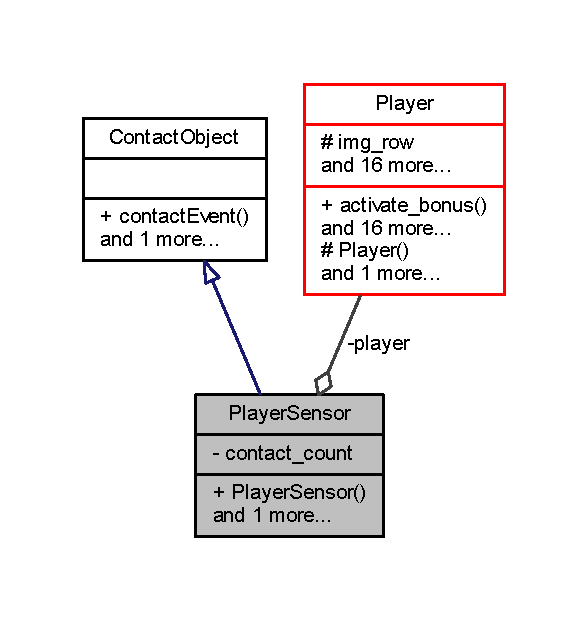
\includegraphics[width=282pt]{class_player_sensor__coll__graph}
\end{center}
\end{figure}
\subsection*{Public Member Functions}
\begin{DoxyCompactItemize}
\item 
\hyperlink{class_player_sensor_a1e74f6ad656f4cdc6449fc55b41dff42}{Player\+Sensor} (\hyperlink{class_player}{Player} $\ast$observable\+\_\+player, b2\+Body $\ast$body)
\begin{DoxyCompactList}\small\item\em Defined constructor for this class. \end{DoxyCompactList}\end{DoxyCompactItemize}
\subsection*{Private Member Functions}
\begin{DoxyCompactItemize}
\item 
\mbox{\Hypertarget{class_player_sensor_a6977b8699ebf0d3d2d2b177665060f21}\label{class_player_sensor_a6977b8699ebf0d3d2d2b177665060f21}} 
void \hyperlink{class_player_sensor_a6977b8699ebf0d3d2d2b177665060f21}{contact\+Event} (b2\+Contact $\ast$contact, bool is\+\_\+begin)
\begin{DoxyCompactList}\small\item\em inhereted from \hyperlink{class_contact_object}{Contact\+Object} \end{DoxyCompactList}\end{DoxyCompactItemize}
\subsection*{Private Attributes}
\begin{DoxyCompactItemize}
\item 
\mbox{\Hypertarget{class_player_sensor_afd6fd57380fc1752edbd601566e52980}\label{class_player_sensor_afd6fd57380fc1752edbd601566e52980}} 
int \hyperlink{class_player_sensor_afd6fd57380fc1752edbd601566e52980}{contact\+\_\+count}
\begin{DoxyCompactList}\small\item\em the number of active contact \end{DoxyCompactList}\item 
\mbox{\Hypertarget{class_player_sensor_a28ca9f490022e0473064290956fe6852}\label{class_player_sensor_a28ca9f490022e0473064290956fe6852}} 
\hyperlink{class_player}{Player} $\ast$ \hyperlink{class_player_sensor_a28ca9f490022e0473064290956fe6852}{player}
\begin{DoxyCompactList}\small\item\em pointer to the player object to which this sensor is attached \end{DoxyCompactList}\end{DoxyCompactItemize}


\subsection{Detailed Description}
Special sensor for character. 

\begin{DoxyAuthor}{Author}
Vasily 
\end{DoxyAuthor}
\begin{DoxyVersion}{Version}
1.\+0 
\end{DoxyVersion}
\begin{DoxyDate}{Date}
June 2017
\end{DoxyDate}
Allow define position of the hero relatively the ground (see on\+\_\+ground in \hyperlink{class_player}{Player} class) 

\subsection{Constructor \& Destructor Documentation}
\mbox{\Hypertarget{class_player_sensor_a1e74f6ad656f4cdc6449fc55b41dff42}\label{class_player_sensor_a1e74f6ad656f4cdc6449fc55b41dff42}} 
\index{Player\+Sensor@{Player\+Sensor}!Player\+Sensor@{Player\+Sensor}}
\index{Player\+Sensor@{Player\+Sensor}!Player\+Sensor@{Player\+Sensor}}
\subsubsection{\texorpdfstring{Player\+Sensor()}{PlayerSensor()}}
{\footnotesize\ttfamily Player\+Sensor\+::\+Player\+Sensor (\begin{DoxyParamCaption}\item[{\hyperlink{class_player}{Player} $\ast$}]{observable\+\_\+player,  }\item[{b2\+Body $\ast$}]{body }\end{DoxyParamCaption})}



Defined constructor for this class. 


\begin{DoxyParams}{Parameters}
{\em observable\+\_\+player} & pointer to the \hyperlink{class_player}{Player} class to which body this sensor is attached \\
\hline
{\em body} & pointer to the box2d body assigned to this sensor \\
\hline
\end{DoxyParams}


The documentation for this class was generated from the following files\+:\begin{DoxyCompactItemize}
\item 
\hyperlink{_player_sensor_8h}{Player\+Sensor.\+h}\item 
Player\+Sensor.\+cpp\end{DoxyCompactItemize}

\hypertarget{class_player_u_i}{}\section{Player\+UI Class Reference}
\label{class_player_u_i}\index{Player\+UI@{Player\+UI}}


Contains the necessary-\/for-\/display information about the hero.  




{\ttfamily \#include $<$Player\+U\+I.\+h$>$}



Collaboration diagram for Player\+UI\+:\nopagebreak
\begin{figure}[H]
\begin{center}
\leavevmode
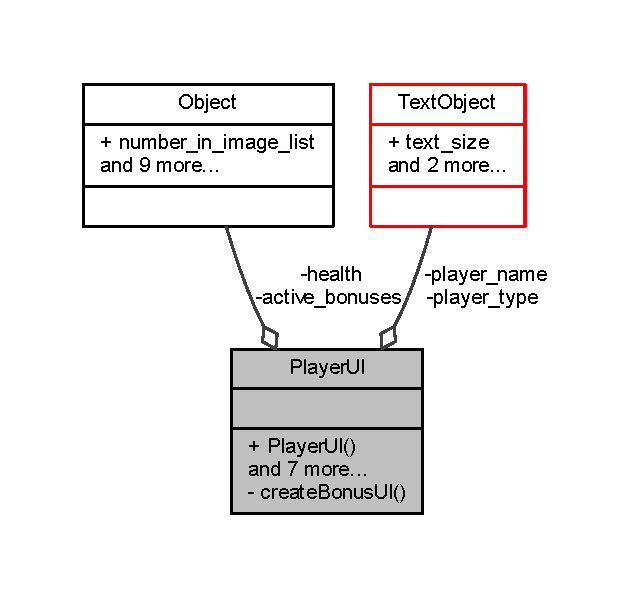
\includegraphics[width=303pt]{class_player_u_i__coll__graph}
\end{center}
\end{figure}
\subsection*{Public Member Functions}
\begin{DoxyCompactItemize}
\item 
\mbox{\Hypertarget{class_player_u_i_a6258658ac25fa64b122bffdf8e1e41fc}\label{class_player_u_i_a6258658ac25fa64b122bffdf8e1e41fc}} 
\hyperlink{class_player_u_i_a6258658ac25fa64b122bffdf8e1e41fc}{Player\+UI} ()
\begin{DoxyCompactList}\small\item\em default constructor \end{DoxyCompactList}\item 
\hyperlink{class_text_object}{Text\+Object} $\ast$ \hyperlink{class_player_u_i_a757ad508c40877d30f9f8b45f8afeccf}{get\+Player\+Name} ()
\item 
\hyperlink{class_text_object}{Text\+Object} $\ast$ \hyperlink{class_player_u_i_a45451abaa9482efb72379df93c2ca37e}{get\+Player\+Type} ()
\item 
void \hyperlink{class_player_u_i_a5cb795f694ec795a49591e6c3a7c7e64}{set\+Health\+Line\+Img} (int i)
\begin{DoxyCompactList}\small\item\em set level of health bar \end{DoxyCompactList}\item 
void \hyperlink{class_player_u_i_ae89b4bc3d9337f7010c504f6dd89e473}{set\+Player\+Name} (std\+::string name)
\item 
void \hyperlink{class_player_u_i_ab43462a4fd71580e29c06f6516f279b4}{set\+Player\+Type} (std\+::string type)
\item 
\hyperlink{class_object}{Object} $\ast$ \hyperlink{class_player_u_i_aebce345a44f53a6ae0a6ac495aa6e17a}{get\+Active\+Bonuses\+Ptr} (int number)
\begin{DoxyCompactList}\small\item\em return bonus \hyperlink{class_object}{Object} from defined ui cell \end{DoxyCompactList}\item 
\hyperlink{class_object}{Object} $\ast$ \hyperlink{class_player_u_i_a013d923f183d6fb7f6e2a2cc2d1dd806}{get\+Health\+Ptr} ()
\end{DoxyCompactItemize}
\subsection*{Private Member Functions}
\begin{DoxyCompactItemize}
\item 
\mbox{\Hypertarget{class_player_u_i_a6d4c17615d2bf85c7db65d6e3557d5f0}\label{class_player_u_i_a6d4c17615d2bf85c7db65d6e3557d5f0}} 
void \hyperlink{class_player_u_i_a6d4c17615d2bf85c7db65d6e3557d5f0}{create\+Bonus\+UI} ()
\begin{DoxyCompactList}\small\item\em Prepares array of bonus cell. \end{DoxyCompactList}\end{DoxyCompactItemize}
\subsection*{Private Attributes}
\begin{DoxyCompactItemize}
\item 
\mbox{\Hypertarget{class_player_u_i_ab9651a40a71fc4c84fad8e3d626a3386}\label{class_player_u_i_ab9651a40a71fc4c84fad8e3d626a3386}} 
\hyperlink{class_text_object}{Text\+Object} \hyperlink{class_player_u_i_ab9651a40a71fc4c84fad8e3d626a3386}{player\+\_\+name}
\begin{DoxyCompactList}\small\item\em player name \end{DoxyCompactList}\item 
\mbox{\Hypertarget{class_player_u_i_a97dbafa8c5c0a651d62d25abbca726a1}\label{class_player_u_i_a97dbafa8c5c0a651d62d25abbca726a1}} 
\hyperlink{class_text_object}{Text\+Object} \hyperlink{class_player_u_i_a97dbafa8c5c0a651d62d25abbca726a1}{player\+\_\+type}
\begin{DoxyCompactList}\small\item\em player type (strong or dexterous) \end{DoxyCompactList}\item 
\mbox{\Hypertarget{class_player_u_i_ae72b43eec4a8060f917d38516e715da2}\label{class_player_u_i_ae72b43eec4a8060f917d38516e715da2}} 
\hyperlink{class_object}{Object} \hyperlink{class_player_u_i_ae72b43eec4a8060f917d38516e715da2}{active\+\_\+bonuses} \mbox{[}3\mbox{]}
\begin{DoxyCompactList}\small\item\em array of bonus cell \end{DoxyCompactList}\item 
\mbox{\Hypertarget{class_player_u_i_a5ca02efb3a04ec5661789dd97d6676fb}\label{class_player_u_i_a5ca02efb3a04ec5661789dd97d6676fb}} 
\hyperlink{class_object}{Object} \hyperlink{class_player_u_i_a5ca02efb3a04ec5661789dd97d6676fb}{health} \{ 0, 0, 0, 28, 52, 10, 99, 0, true, 255 \}
\begin{DoxyCompactList}\small\item\em health bar \end{DoxyCompactList}\end{DoxyCompactItemize}


\subsection{Detailed Description}
Contains the necessary-\/for-\/display information about the hero. 

\begin{DoxyAuthor}{Author}
Vasily 
\end{DoxyAuthor}
\begin{DoxyVersion}{Version}
1.\+0 
\end{DoxyVersion}
\begin{DoxyDate}{Date}
June 2017 
\end{DoxyDate}


\subsection{Member Function Documentation}
\mbox{\Hypertarget{class_player_u_i_aebce345a44f53a6ae0a6ac495aa6e17a}\label{class_player_u_i_aebce345a44f53a6ae0a6ac495aa6e17a}} 
\index{Player\+UI@{Player\+UI}!get\+Active\+Bonuses\+Ptr@{get\+Active\+Bonuses\+Ptr}}
\index{get\+Active\+Bonuses\+Ptr@{get\+Active\+Bonuses\+Ptr}!Player\+UI@{Player\+UI}}
\subsubsection{\texorpdfstring{get\+Active\+Bonuses\+Ptr()}{getActiveBonusesPtr()}}
{\footnotesize\ttfamily \hyperlink{class_object}{Object} $\ast$ Player\+U\+I\+::get\+Active\+Bonuses\+Ptr (\begin{DoxyParamCaption}\item[{int}]{number }\end{DoxyParamCaption})}



return bonus \hyperlink{class_object}{Object} from defined ui cell 


\begin{DoxyParams}{Parameters}
{\em number} & cell-\/number \\
\hline
\end{DoxyParams}
\begin{DoxyReturn}{Returns}
bonus \hyperlink{class_object}{Object} in this cell 
\end{DoxyReturn}
\mbox{\Hypertarget{class_player_u_i_a013d923f183d6fb7f6e2a2cc2d1dd806}\label{class_player_u_i_a013d923f183d6fb7f6e2a2cc2d1dd806}} 
\index{Player\+UI@{Player\+UI}!get\+Health\+Ptr@{get\+Health\+Ptr}}
\index{get\+Health\+Ptr@{get\+Health\+Ptr}!Player\+UI@{Player\+UI}}
\subsubsection{\texorpdfstring{get\+Health\+Ptr()}{getHealthPtr()}}
{\footnotesize\ttfamily \hyperlink{class_object}{Object} $\ast$ Player\+U\+I\+::get\+Health\+Ptr (\begin{DoxyParamCaption}{ }\end{DoxyParamCaption})}

\begin{DoxyReturn}{Returns}
health bar \hyperlink{class_object}{Object} 
\end{DoxyReturn}
\mbox{\Hypertarget{class_player_u_i_a757ad508c40877d30f9f8b45f8afeccf}\label{class_player_u_i_a757ad508c40877d30f9f8b45f8afeccf}} 
\index{Player\+UI@{Player\+UI}!get\+Player\+Name@{get\+Player\+Name}}
\index{get\+Player\+Name@{get\+Player\+Name}!Player\+UI@{Player\+UI}}
\subsubsection{\texorpdfstring{get\+Player\+Name()}{getPlayerName()}}
{\footnotesize\ttfamily \hyperlink{class_text_object}{Text\+Object} $\ast$ Player\+U\+I\+::get\+Player\+Name (\begin{DoxyParamCaption}{ }\end{DoxyParamCaption})}

\begin{DoxyReturn}{Returns}
\hyperlink{class_text_object}{Text\+Object} with player name 
\end{DoxyReturn}
\mbox{\Hypertarget{class_player_u_i_a45451abaa9482efb72379df93c2ca37e}\label{class_player_u_i_a45451abaa9482efb72379df93c2ca37e}} 
\index{Player\+UI@{Player\+UI}!get\+Player\+Type@{get\+Player\+Type}}
\index{get\+Player\+Type@{get\+Player\+Type}!Player\+UI@{Player\+UI}}
\subsubsection{\texorpdfstring{get\+Player\+Type()}{getPlayerType()}}
{\footnotesize\ttfamily \hyperlink{class_text_object}{Text\+Object} $\ast$ Player\+U\+I\+::get\+Player\+Type (\begin{DoxyParamCaption}{ }\end{DoxyParamCaption})}

\begin{DoxyReturn}{Returns}
\hyperlink{class_text_object}{Text\+Object} with player type 
\end{DoxyReturn}
\mbox{\Hypertarget{class_player_u_i_a5cb795f694ec795a49591e6c3a7c7e64}\label{class_player_u_i_a5cb795f694ec795a49591e6c3a7c7e64}} 
\index{Player\+UI@{Player\+UI}!set\+Health\+Line\+Img@{set\+Health\+Line\+Img}}
\index{set\+Health\+Line\+Img@{set\+Health\+Line\+Img}!Player\+UI@{Player\+UI}}
\subsubsection{\texorpdfstring{set\+Health\+Line\+Img()}{setHealthLineImg()}}
{\footnotesize\ttfamily void Player\+U\+I\+::set\+Health\+Line\+Img (\begin{DoxyParamCaption}\item[{int}]{i }\end{DoxyParamCaption})}



set level of health bar 


\begin{DoxyParams}{Parameters}
{\em i} & level of hero health \\
\hline
\end{DoxyParams}
\mbox{\Hypertarget{class_player_u_i_ae89b4bc3d9337f7010c504f6dd89e473}\label{class_player_u_i_ae89b4bc3d9337f7010c504f6dd89e473}} 
\index{Player\+UI@{Player\+UI}!set\+Player\+Name@{set\+Player\+Name}}
\index{set\+Player\+Name@{set\+Player\+Name}!Player\+UI@{Player\+UI}}
\subsubsection{\texorpdfstring{set\+Player\+Name()}{setPlayerName()}}
{\footnotesize\ttfamily void Player\+U\+I\+::set\+Player\+Name (\begin{DoxyParamCaption}\item[{std\+::string}]{name }\end{DoxyParamCaption})}


\begin{DoxyParams}{Parameters}
{\em name} & player name \\
\hline
\end{DoxyParams}
\mbox{\Hypertarget{class_player_u_i_ab43462a4fd71580e29c06f6516f279b4}\label{class_player_u_i_ab43462a4fd71580e29c06f6516f279b4}} 
\index{Player\+UI@{Player\+UI}!set\+Player\+Type@{set\+Player\+Type}}
\index{set\+Player\+Type@{set\+Player\+Type}!Player\+UI@{Player\+UI}}
\subsubsection{\texorpdfstring{set\+Player\+Type()}{setPlayerType()}}
{\footnotesize\ttfamily void Player\+U\+I\+::set\+Player\+Type (\begin{DoxyParamCaption}\item[{std\+::string}]{type }\end{DoxyParamCaption})}


\begin{DoxyParams}{Parameters}
{\em type} & player type \\
\hline
\end{DoxyParams}


The documentation for this class was generated from the following files\+:\begin{DoxyCompactItemize}
\item 
\hyperlink{_player_u_i_8h}{Player\+U\+I.\+h}\item 
Player\+U\+I.\+cpp\end{DoxyCompactItemize}

\hypertarget{struct_position_relatively_screen}{}\section{Position\+Relatively\+Screen Struct Reference}
\label{struct_position_relatively_screen}\index{Position\+Relatively\+Screen@{Position\+Relatively\+Screen}}


Collaboration diagram for Position\+Relatively\+Screen\+:\nopagebreak
\begin{figure}[H]
\begin{center}
\leavevmode
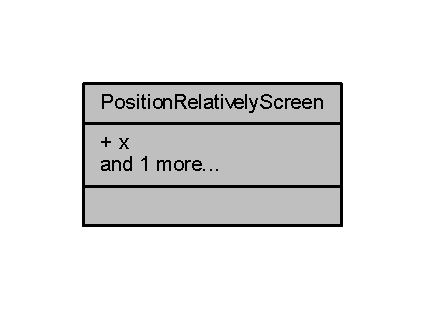
\includegraphics[width=204pt]{struct_position_relatively_screen__coll__graph}
\end{center}
\end{figure}
\subsection*{Static Public Attributes}
\begin{DoxyCompactItemize}
\item 
\mbox{\Hypertarget{struct_position_relatively_screen_ac1e997b81f9705f4a76f1bf9df9f9fd9}\label{struct_position_relatively_screen_ac1e997b81f9705f4a76f1bf9df9f9fd9}} 
static double {\bfseries x} = 0
\item 
\mbox{\Hypertarget{struct_position_relatively_screen_a1b0b578732e926941d2b5533bcc16c62}\label{struct_position_relatively_screen_a1b0b578732e926941d2b5533bcc16c62}} 
static double {\bfseries y} = 0
\end{DoxyCompactItemize}


The documentation for this struct was generated from the following files\+:\begin{DoxyCompactItemize}
\item 
Events.\+h\item 
Events.\+cpp\end{DoxyCompactItemize}

\hypertarget{class_revolute_bridge}{}\section{Revolute\+Bridge Class Reference}
\label{class_revolute_bridge}\index{Revolute\+Bridge@{Revolute\+Bridge}}


Drawbridge which can be activated by the sensor.  




{\ttfamily \#include $<$Revolute\+Bridge.\+h$>$}



Collaboration diagram for Revolute\+Bridge\+:\nopagebreak
\begin{figure}[H]
\begin{center}
\leavevmode
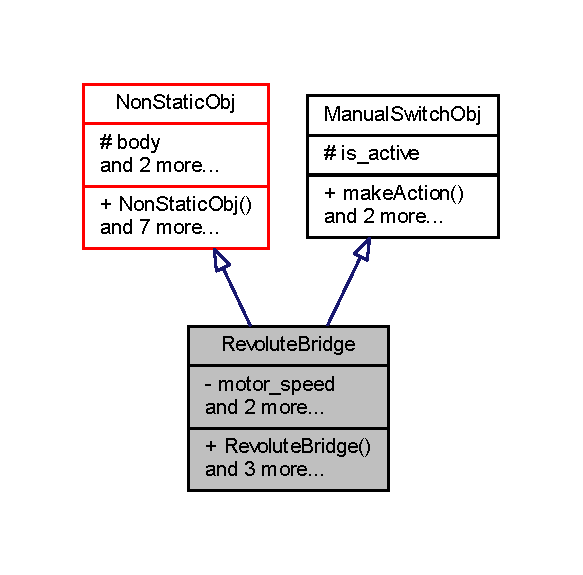
\includegraphics[width=280pt]{class_revolute_bridge__coll__graph}
\end{center}
\end{figure}
\subsection*{Public Member Functions}
\begin{DoxyCompactItemize}
\item 
\hyperlink{class_revolute_bridge_a2b0f68222d155f93018b85bd5629c4b4}{Revolute\+Bridge} (b2\+Body $\ast$\+\_\+body, \hyperlink{class_object}{Object} $\ast$\+\_\+object, b2\+Revolute\+Joint $\ast$\+\_\+bridge\+\_\+joint, double \+\_\+motor\+\_\+speed)
\begin{DoxyCompactList}\small\item\em Defined constructor for this class. \end{DoxyCompactList}\item 
\mbox{\Hypertarget{class_revolute_bridge_aad7a57a94ab4bd41cd4e1da48d627d00}\label{class_revolute_bridge_aad7a57a94ab4bd41cd4e1da48d627d00}} 
void \hyperlink{class_revolute_bridge_aad7a57a94ab4bd41cd4e1da48d627d00}{make\+Action} (\hyperlink{_manual_switch_obj_8h_a8bb1ef53467e4f61410d12822d922498}{Action} action)
\begin{DoxyCompactList}\small\item\em inhereted from \hyperlink{class_manual_switch_obj}{Manual\+Switch\+Obj} class \end{DoxyCompactList}\item 
\mbox{\Hypertarget{class_revolute_bridge_ae3777840011c40e126e6e3fce4706f9a}\label{class_revolute_bridge_ae3777840011c40e126e6e3fce4706f9a}} 
bool \hyperlink{class_revolute_bridge_ae3777840011c40e126e6e3fce4706f9a}{destroy} ()
\begin{DoxyCompactList}\small\item\em inhereted from \hyperlink{class_non_static_obj}{Non\+Static\+Obj} class \end{DoxyCompactList}\item 
\mbox{\Hypertarget{class_revolute_bridge_ac462a7308f806d30c53e35b2b8a57e5d}\label{class_revolute_bridge_ac462a7308f806d30c53e35b2b8a57e5d}} 
void \hyperlink{class_revolute_bridge_ac462a7308f806d30c53e35b2b8a57e5d}{update} ()
\begin{DoxyCompactList}\small\item\em inhereted from \hyperlink{class_non_static_obj}{Non\+Static\+Obj} class \end{DoxyCompactList}\end{DoxyCompactItemize}
\subsection*{Private Attributes}
\begin{DoxyCompactItemize}
\item 
\mbox{\Hypertarget{class_revolute_bridge_a43f73302f3cf2296ef6693244af857c9}\label{class_revolute_bridge_a43f73302f3cf2296ef6693244af857c9}} 
double \hyperlink{class_revolute_bridge_a43f73302f3cf2296ef6693244af857c9}{motor\+\_\+speed}
\begin{DoxyCompactList}\small\item\em speed of bridge rotation \end{DoxyCompactList}\item 
\mbox{\Hypertarget{class_revolute_bridge_a2a2330cd9538b2d2f049710494648de9}\label{class_revolute_bridge_a2a2330cd9538b2d2f049710494648de9}} 
b2\+Revolute\+Joint $\ast$ \hyperlink{class_revolute_bridge_a2a2330cd9538b2d2f049710494648de9}{joint}
\begin{DoxyCompactList}\small\item\em pointer to the box2d joint where bridge pin to the world ground \end{DoxyCompactList}\item 
\mbox{\Hypertarget{class_revolute_bridge_a2acc242725606650e33a98f3d8f0b382}\label{class_revolute_bridge_a2acc242725606650e33a98f3d8f0b382}} 
bool \hyperlink{class_revolute_bridge_a2acc242725606650e33a98f3d8f0b382}{is\+\_\+joint\+\_\+exist}
\begin{DoxyCompactList}\small\item\em define joint existense \textquotesingle{}true\textquotesingle{} -\/ exist; \textquotesingle{}false\textquotesingle{} -\/ dosen\textquotesingle{}t exist \end{DoxyCompactList}\end{DoxyCompactItemize}
\subsection*{Additional Inherited Members}


\subsection{Detailed Description}
Drawbridge which can be activated by the sensor. 

\begin{DoxyAuthor}{Author}
Vasily 
\end{DoxyAuthor}
\begin{DoxyVersion}{Version}
1.\+0 
\end{DoxyVersion}
\begin{DoxyDate}{Date}
June 2017 
\end{DoxyDate}


\subsection{Constructor \& Destructor Documentation}
\mbox{\Hypertarget{class_revolute_bridge_a2b0f68222d155f93018b85bd5629c4b4}\label{class_revolute_bridge_a2b0f68222d155f93018b85bd5629c4b4}} 
\index{Revolute\+Bridge@{Revolute\+Bridge}!Revolute\+Bridge@{Revolute\+Bridge}}
\index{Revolute\+Bridge@{Revolute\+Bridge}!Revolute\+Bridge@{Revolute\+Bridge}}
\subsubsection{\texorpdfstring{Revolute\+Bridge()}{RevoluteBridge()}}
{\footnotesize\ttfamily Revolute\+Bridge\+::\+Revolute\+Bridge (\begin{DoxyParamCaption}\item[{b2\+Body $\ast$}]{\+\_\+body,  }\item[{\hyperlink{class_object}{Object} $\ast$}]{\+\_\+object,  }\item[{b2\+Revolute\+Joint $\ast$}]{\+\_\+bridge\+\_\+joint,  }\item[{double}]{\+\_\+motor\+\_\+speed }\end{DoxyParamCaption})}



Defined constructor for this class. 


\begin{DoxyParams}{Parameters}
{\em \+\_\+body} & pointer to the box2d body assigned to this bridge \\
\hline
{\em \+\_\+object} & pointer to the \hyperlink{class_object}{Object} class assigned to this bridge \\
\hline
{\em \+\_\+bridge\+\_\+joint} & pointer to the \hyperlink{class_viewer}{Viewer} class, which will use in M\+VC model \\
\hline
{\em \+\_\+motor\+\_\+speed} & speed of bridge rotation \\
\hline
\end{DoxyParams}


The documentation for this class was generated from the following files\+:\begin{DoxyCompactItemize}
\item 
\hyperlink{_revolute_bridge_8h}{Revolute\+Bridge.\+h}\item 
Revolute\+Bridge.\+cpp\end{DoxyCompactItemize}

\hypertarget{class_sensor}{}\section{Sensor Class Reference}
\label{class_sensor}\index{Sensor@{Sensor}}


Trigger that can activate observables \hyperlink{class_manual_switch_obj}{Manual\+Switch\+Obj} classes (dosen\textquotesingle{}t display at the monitor)  




{\ttfamily \#include $<$Sensor.\+h$>$}



Collaboration diagram for Sensor\+:
\nopagebreak
\begin{figure}[H]
\begin{center}
\leavevmode
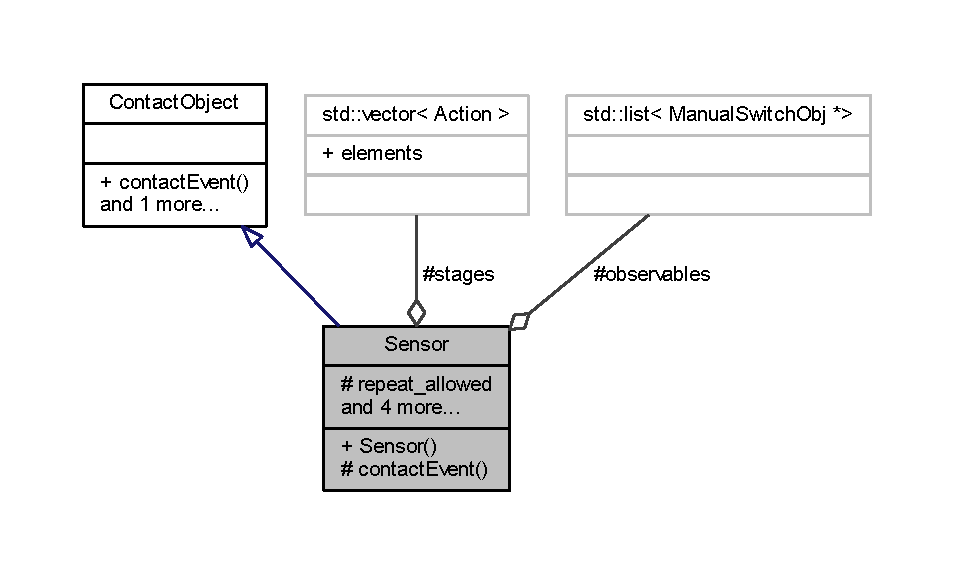
\includegraphics[width=350pt]{class_sensor__coll__graph}
\end{center}
\end{figure}
\subsection*{Public Member Functions}
\begin{DoxyCompactItemize}
\item 
\hyperlink{class_sensor_a7988853c8a9278171ce8956ccdde63c8}{Sensor} (std\+::list$<$ \hyperlink{class_manual_switch_obj}{Manual\+Switch\+Obj} $\ast$$>$ \+\_\+observables, bool \+\_\+repeat\+\_\+allowed, bool \+\_\+is\+\_\+keeping, b2\+Body $\ast$\+\_\+body, std\+::vector$<$ \hyperlink{_manual_switch_obj_8h_a8bb1ef53467e4f61410d12822d922498}{Action} $>$ \+\_\+stages)
\begin{DoxyCompactList}\small\item\em Defined constructor for this class. \end{DoxyCompactList}\end{DoxyCompactItemize}
\subsection*{Protected Member Functions}
\begin{DoxyCompactItemize}
\item 
\mbox{\Hypertarget{class_sensor_a3445be09d7e8905b1d8e46f2e0306542}\label{class_sensor_a3445be09d7e8905b1d8e46f2e0306542}} 
virtual void \hyperlink{class_sensor_a3445be09d7e8905b1d8e46f2e0306542}{contact\+Event} (b2\+Contact $\ast$contact, bool is\+\_\+begin)
\begin{DoxyCompactList}\small\item\em inherited from \hyperlink{class_contact_object}{Contact\+Object} class \end{DoxyCompactList}\end{DoxyCompactItemize}
\subsection*{Protected Attributes}
\begin{DoxyCompactItemize}
\item 
\mbox{\Hypertarget{class_sensor_a3056529f52d9af83b78bc7ca7e2e7ef2}\label{class_sensor_a3056529f52d9af83b78bc7ca7e2e7ef2}} 
std\+::list$<$ \hyperlink{class_manual_switch_obj}{Manual\+Switch\+Obj} $\ast$ $>$ \hyperlink{class_sensor_a3056529f52d9af83b78bc7ca7e2e7ef2}{observables}
\begin{DoxyCompactList}\small\item\em list of observables objects \end{DoxyCompactList}\item 
\mbox{\Hypertarget{class_sensor_a2450a980532d0448e7ea1f9db91f79f7}\label{class_sensor_a2450a980532d0448e7ea1f9db91f79f7}} 
std\+::vector$<$ \hyperlink{_manual_switch_obj_8h_a8bb1ef53467e4f61410d12822d922498}{Action} $>$ \hyperlink{class_sensor_a2450a980532d0448e7ea1f9db91f79f7}{stages}
\begin{DoxyCompactList}\small\item\em vector of stages(commands) through which observables objects should pass \end{DoxyCompactList}\item 
\mbox{\Hypertarget{class_sensor_a8554cb0f6e9cfcc6f277795bdd45ce14}\label{class_sensor_a8554cb0f6e9cfcc6f277795bdd45ce14}} 
bool \hyperlink{class_sensor_a8554cb0f6e9cfcc6f277795bdd45ce14}{repeat\+\_\+allowed}
\begin{DoxyCompactList}\small\item\em determines whether it is possible to send next command to the observables objects when they doesn\textquotesingle{}t complete previous action\+: \textquotesingle{}true\textquotesingle{} -\/ possible; \textquotesingle{}false\textquotesingle{} -\/ impossible \end{DoxyCompactList}\item 
\mbox{\Hypertarget{class_sensor_ace9f91b1e1034b501ba8f16e46b61698}\label{class_sensor_ace9f91b1e1034b501ba8f16e46b61698}} 
bool \hyperlink{class_sensor_ace9f91b1e1034b501ba8f16e46b61698}{is\+\_\+keeping}
\begin{DoxyCompactList}\small\item\em determines will be next command send afther end of the contact(end of the hold button)\+: \textquotesingle{}true\textquotesingle{} -\/ will be; \textquotesingle{}false\textquotesingle{} -\/ won\textquotesingle{}t be \end{DoxyCompactList}\item 
\mbox{\Hypertarget{class_sensor_a40badc87a0a663f3bcbc95867b6f6296}\label{class_sensor_a40badc87a0a663f3bcbc95867b6f6296}} 
bool \hyperlink{class_sensor_a40badc87a0a663f3bcbc95867b6f6296}{non\+\_\+run}
\begin{DoxyCompactList}\small\item\em contain information about valid of the last contact\+: \textquotesingle{}true\textquotesingle{} -\/ sensor didn\textquotesingle{}t respond; \textquotesingle{}false\textquotesingle{} -\/ sensor responded \end{DoxyCompactList}\item 
\mbox{\Hypertarget{class_sensor_aff0be53ae0ed2e7f2a34e93bd78eed5d}\label{class_sensor_aff0be53ae0ed2e7f2a34e93bd78eed5d}} 
int \hyperlink{class_sensor_aff0be53ae0ed2e7f2a34e93bd78eed5d}{is\+\_\+pressed}
\begin{DoxyCompactList}\small\item\em number of active contacts \end{DoxyCompactList}\item 
\mbox{\Hypertarget{class_sensor_aaf93d0f69a770e911edaf5f265eec623}\label{class_sensor_aaf93d0f69a770e911edaf5f265eec623}} 
int \hyperlink{class_sensor_aaf93d0f69a770e911edaf5f265eec623}{stage\+\_\+iter}
\begin{DoxyCompactList}\small\item\em number of current stage from stages vector \end{DoxyCompactList}\end{DoxyCompactItemize}


\subsection{Detailed Description}
Trigger that can activate observables \hyperlink{class_manual_switch_obj}{Manual\+Switch\+Obj} classes (dosen\textquotesingle{}t display at the monitor) 

\begin{DoxyAuthor}{Author}
Vasily 
\end{DoxyAuthor}
\begin{DoxyVersion}{Version}
1.\+0 
\end{DoxyVersion}
\begin{DoxyDate}{Date}
June 2017 
\end{DoxyDate}


\subsection{Constructor \& Destructor Documentation}
\mbox{\Hypertarget{class_sensor_a7988853c8a9278171ce8956ccdde63c8}\label{class_sensor_a7988853c8a9278171ce8956ccdde63c8}} 
\index{Sensor@{Sensor}!Sensor@{Sensor}}
\index{Sensor@{Sensor}!Sensor@{Sensor}}
\subsubsection{\texorpdfstring{Sensor()}{Sensor()}}
{\footnotesize\ttfamily Sensor\+::\+Sensor (\begin{DoxyParamCaption}\item[{std\+::list$<$ \hyperlink{class_manual_switch_obj}{Manual\+Switch\+Obj} $\ast$$>$}]{\+\_\+observables,  }\item[{bool}]{\+\_\+repeat\+\_\+allowed,  }\item[{bool}]{\+\_\+is\+\_\+keeping,  }\item[{b2\+Body $\ast$}]{\+\_\+body,  }\item[{std\+::vector$<$ \hyperlink{_manual_switch_obj_8h_a8bb1ef53467e4f61410d12822d922498}{Action} $>$}]{\+\_\+stages }\end{DoxyParamCaption})}



Defined constructor for this class. 


\begin{DoxyParams}{Parameters}
{\em \+\_\+observables} & list of observables objects \\
\hline
{\em \+\_\+repeat\+\_\+allowed} & determines whether it is possible to send next command to the observables objects when they doesn\textquotesingle{}t complete previous action\+: \textquotesingle{}true\textquotesingle{} -\/ possible; \textquotesingle{}false\textquotesingle{} -\/ impossible \\
\hline
{\em \+\_\+is\+\_\+keeping} & determines will be next command send afther end of the contact(end of the hold button)\+: \textquotesingle{}true\textquotesingle{} -\/ will be; \textquotesingle{}false\textquotesingle{} -\/ won\textquotesingle{}t be \\
\hline
{\em \+\_\+body} & pointer to the box2d body assigned to this sensor \\
\hline
{\em \+\_\+stages} & vector of stages(commands) through which observables objects should pass \\
\hline
\end{DoxyParams}


The documentation for this class was generated from the following files\+:\begin{DoxyCompactItemize}
\item 
\hyperlink{_sensor_8h}{Sensor.\+h}\item 
Sensor.\+cpp\end{DoxyCompactItemize}

\hypertarget{class_storage}{}\section{Storage Class Reference}
\label{class_storage}\index{Storage@{Storage}}


Collaboration diagram for Storage\+:\nopagebreak
\begin{figure}[H]
\begin{center}
\leavevmode
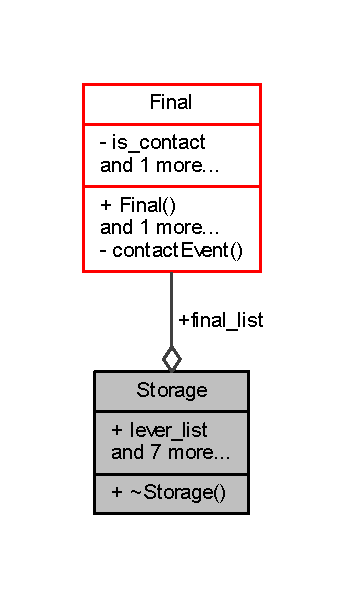
\includegraphics[width=168pt]{class_storage__coll__graph}
\end{center}
\end{figure}
\subsection*{Public Attributes}
\begin{DoxyCompactItemize}
\item 
\mbox{\Hypertarget{class_storage_a183e52c6e96e3174e51b6ae47579ed55}\label{class_storage_a183e52c6e96e3174e51b6ae47579ed55}} 
std\+::list$<$ \hyperlink{class_lever}{Lever} $\ast$ $>$ {\bfseries lever\+\_\+list}
\item 
\mbox{\Hypertarget{class_storage_a9d200f7ba37543482bd1a50a54063ace}\label{class_storage_a9d200f7ba37543482bd1a50a54063ace}} 
std\+::list$<$ \hyperlink{class_timer}{Timer} $\ast$ $>$ {\bfseries timer\+\_\+list}
\item 
\mbox{\Hypertarget{class_storage_af0e098198f6896d667ce135b5d81b7c1}\label{class_storage_af0e098198f6896d667ce135b5d81b7c1}} 
std\+::list$<$ \hyperlink{class_non_static_obj}{Non\+Static\+Obj} $\ast$ $>$ {\bfseries non\+\_\+static\+\_\+objects}
\item 
\mbox{\Hypertarget{class_storage_a9003cf58d8b5c48ca1ac7d0ce7323238}\label{class_storage_a9003cf58d8b5c48ca1ac7d0ce7323238}} 
std\+::list$<$ \hyperlink{class_player_sensor}{Player\+Sensor} $\ast$ $>$ {\bfseries players\+\_\+sensors\+\_\+list}
\item 
\mbox{\Hypertarget{class_storage_ad96cf086d9e0eb5b811504d26737f351}\label{class_storage_ad96cf086d9e0eb5b811504d26737f351}} 
std\+::list$<$ \hyperlink{class_non_static_obj}{Non\+Static\+Obj} $\ast$ $>$ $\ast$ {\bfseries to\+\_\+destroy\+\_\+list}
\item 
\mbox{\Hypertarget{class_storage_a6cb1b8c7f32484e515530c7eb54ed08f}\label{class_storage_a6cb1b8c7f32484e515530c7eb54ed08f}} 
std\+::list$<$ \hyperlink{class_danger_object}{Danger\+Object} $\ast$ $>$ {\bfseries danger\+\_\+list}
\item 
\mbox{\Hypertarget{class_storage_aca489d11da5a79c4ada94fb89aebab69}\label{class_storage_aca489d11da5a79c4ada94fb89aebab69}} 
\hyperlink{class_final}{Final} $\ast$ {\bfseries final\+\_\+list} \mbox{[}2\mbox{]}
\item 
\mbox{\Hypertarget{class_storage_a16492ba80ed615d1b917a12d8a959fed}\label{class_storage_a16492ba80ed615d1b917a12d8a959fed}} 
std\+::list$<$ \hyperlink{class_bonus}{Bonus} $\ast$ $>$ {\bfseries bonus\+\_\+list}
\item 
\mbox{\Hypertarget{class_storage_a9ec3b712f9c20c9c2e82cc07f77ad692}\label{class_storage_a9ec3b712f9c20c9c2e82cc07f77ad692}} 
std\+::map$<$ std\+::string, \hyperlink{class_manual_switch_obj}{Manual\+Switch\+Obj} $\ast$ $>$ {\bfseries future\+\_\+observables}
\end{DoxyCompactItemize}


The documentation for this class was generated from the following file\+:\begin{DoxyCompactItemize}
\item 
Level\+Storage.\+h\end{DoxyCompactItemize}

\hypertarget{class_strong_player}{}\section{Strong\+Player Class Reference}
\label{class_strong_player}\index{Strong\+Player@{Strong\+Player}}


Contains information about strong characret.  




{\ttfamily \#include $<$Strong\+Player.\+h$>$}



Collaboration diagram for Strong\+Player\+:\nopagebreak
\begin{figure}[H]
\begin{center}
\leavevmode
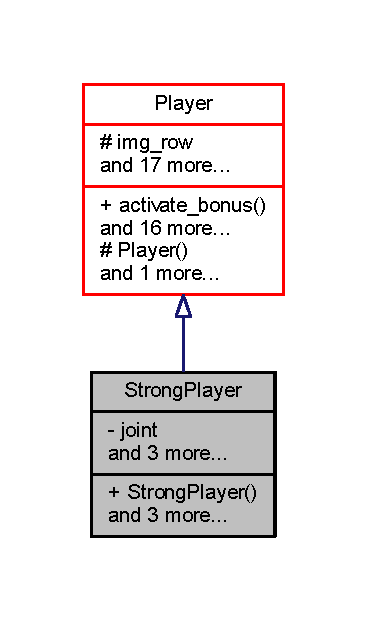
\includegraphics[width=176pt]{class_strong_player__coll__graph}
\end{center}
\end{figure}
\subsection*{Public Member Functions}
\begin{DoxyCompactItemize}
\item 
\hyperlink{class_strong_player_ad8c557c1ae5ada0ce8676c601b16653d}{Strong\+Player} (int \+\_\+level\+\_\+width, int \+\_\+level\+\_\+height, b2\+Body $\ast$\+\_\+body, \hyperlink{class_object}{Object} $\ast$\+\_\+object, int \+\_\+health, Return\+Events $\ast$\+\_\+re)
\begin{DoxyCompactList}\small\item\em Defined constructor for this class. \end{DoxyCompactList}\item 
\mbox{\Hypertarget{class_strong_player_acdae803bf66f620bc73b105ca06c46ab}\label{class_strong_player_acdae803bf66f620bc73b105ca06c46ab}} 
void \hyperlink{class_strong_player_acdae803bf66f620bc73b105ca06c46ab}{try\+To\+Pickup\+Box} ()
\begin{DoxyCompactList}\small\item\em causes the hero to try pick up the box \end{DoxyCompactList}\item 
void \hyperlink{class_strong_player_afb33164ecdb89f91cb32c9b59c6805d1}{throw\+Box} (double x, double y)
\begin{DoxyCompactList}\small\item\em set throwing direction of the box \end{DoxyCompactList}\item 
\mbox{\Hypertarget{class_strong_player_a2e9ec64367e36c1bef0e30293706c1ab}\label{class_strong_player_a2e9ec64367e36c1bef0e30293706c1ab}} 
void \hyperlink{class_strong_player_a2e9ec64367e36c1bef0e30293706c1ab}{update} ()
\begin{DoxyCompactList}\small\item\em inhereted from \hyperlink{class_player}{Player} \end{DoxyCompactList}\end{DoxyCompactItemize}
\subsection*{Private Attributes}
\begin{DoxyCompactItemize}
\item 
\mbox{\Hypertarget{class_strong_player_a4fc2a7b6a98d9f4d9bf7fc5d0d207ba8}\label{class_strong_player_a4fc2a7b6a98d9f4d9bf7fc5d0d207ba8}} 
b2\+Joint $\ast$ \hyperlink{class_strong_player_a4fc2a7b6a98d9f4d9bf7fc5d0d207ba8}{joint}
\begin{DoxyCompactList}\small\item\em pointer to box2d joint which created when hero raises an box \end{DoxyCompactList}\item 
\mbox{\Hypertarget{class_strong_player_a620cdfef8e86100906f5428830bc0508}\label{class_strong_player_a620cdfef8e86100906f5428830bc0508}} 
b2\+Body $\ast$ \hyperlink{class_strong_player_a620cdfef8e86100906f5428830bc0508}{box}
\begin{DoxyCompactList}\small\item\em pointer to box2d body of raised box \end{DoxyCompactList}\item 
\mbox{\Hypertarget{class_strong_player_aa5869805ce789b52b40d6cc47ce23b93}\label{class_strong_player_aa5869805ce789b52b40d6cc47ce23b93}} 
double \hyperlink{class_strong_player_aa5869805ce789b52b40d6cc47ce23b93}{box\+\_\+coef}
\begin{DoxyCompactList}\small\item\em maximum box2d impulse below which hero can carry a box (in other words max mass of the box) \end{DoxyCompactList}\item 
\mbox{\Hypertarget{class_strong_player_a2556cd73a7a49ffe0aa24f300a9faeef}\label{class_strong_player_a2556cd73a7a49ffe0aa24f300a9faeef}} 
bool \hyperlink{class_strong_player_a2556cd73a7a49ffe0aa24f300a9faeef}{is\+\_\+joint\+\_\+set}
\begin{DoxyCompactList}\small\item\em define joint existense \textquotesingle{}true\textquotesingle{} -\/ hero carry a box; \textquotesingle{}false\textquotesingle{} -\/ hero dosen\textquotesingle{}t carry the box \end{DoxyCompactList}\end{DoxyCompactItemize}
\subsection*{Additional Inherited Members}


\subsection{Detailed Description}
Contains information about strong characret. 

\begin{DoxyAuthor}{Author}
Vasily 
\end{DoxyAuthor}
\begin{DoxyVersion}{Version}
1.\+0 
\end{DoxyVersion}
\begin{DoxyDate}{Date}
June 2017 
\end{DoxyDate}


\subsection{Constructor \& Destructor Documentation}
\mbox{\Hypertarget{class_strong_player_ad8c557c1ae5ada0ce8676c601b16653d}\label{class_strong_player_ad8c557c1ae5ada0ce8676c601b16653d}} 
\index{Strong\+Player@{Strong\+Player}!Strong\+Player@{Strong\+Player}}
\index{Strong\+Player@{Strong\+Player}!Strong\+Player@{Strong\+Player}}
\subsubsection{\texorpdfstring{Strong\+Player()}{StrongPlayer()}}
{\footnotesize\ttfamily Strong\+Player\+::\+Strong\+Player (\begin{DoxyParamCaption}\item[{int}]{\+\_\+level\+\_\+width,  }\item[{int}]{\+\_\+level\+\_\+height,  }\item[{b2\+Body $\ast$}]{\+\_\+body,  }\item[{\hyperlink{class_object}{Object} $\ast$}]{\+\_\+object,  }\item[{int}]{\+\_\+health,  }\item[{Return\+Events $\ast$}]{\+\_\+re }\end{DoxyParamCaption})}



Defined constructor for this class. 


\begin{DoxyParams}{Parameters}
{\em \+\_\+level\+\_\+width} & the width in pixels of this level \\
\hline
{\em \+\_\+level\+\_\+height} & the height in pixels of this level \\
\hline
{\em \+\_\+body} & pointer to the box2d body assigned to this character \\
\hline
{\em \+\_\+object} & pointer to the \hyperlink{class_object}{Object} class assigned to this character \\
\hline
{\em \+\_\+health} & the maximum level of health reserve for this caracter \\
\hline
{\em \+\_\+re} & pointer to the variable which contains reply of the current level during last iteration (see \hyperlink{class_layer}{Layer} class) \\
\hline
\end{DoxyParams}


\subsection{Member Function Documentation}
\mbox{\Hypertarget{class_strong_player_afb33164ecdb89f91cb32c9b59c6805d1}\label{class_strong_player_afb33164ecdb89f91cb32c9b59c6805d1}} 
\index{Strong\+Player@{Strong\+Player}!throw\+Box@{throw\+Box}}
\index{throw\+Box@{throw\+Box}!Strong\+Player@{Strong\+Player}}
\subsubsection{\texorpdfstring{throw\+Box()}{throwBox()}}
{\footnotesize\ttfamily void Strong\+Player\+::throw\+Box (\begin{DoxyParamCaption}\item[{double}]{x,  }\item[{double}]{y }\end{DoxyParamCaption})}



set throwing direction of the box 


\begin{DoxyParams}{Parameters}
{\em x} & x coordinate of the direction (will be normalized) \\
\hline
{\em y} & y coordinate of the direction (will be normalized) \\
\hline
\end{DoxyParams}


The documentation for this class was generated from the following files\+:\begin{DoxyCompactItemize}
\item 
\hyperlink{_strong_player_8h}{Strong\+Player.\+h}\item 
Strong\+Player.\+cpp\end{DoxyCompactItemize}

\hypertarget{class_text_object}{}\section{Text\+Object Class Reference}
\label{class_text_object}\index{Text\+Object@{Text\+Object}}


Contains based information about text entity which necessary both for \hyperlink{class_model}{Model} and \hyperlink{class_viewer}{Viewer} classes.  




{\ttfamily \#include $<$Level\+Box.\+h$>$}



Collaboration diagram for Text\+Object\+:
\nopagebreak
\begin{figure}[H]
\begin{center}
\leavevmode
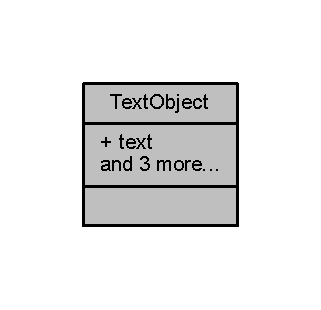
\includegraphics[width=154pt]{class_text_object__coll__graph}
\end{center}
\end{figure}
\subsection*{Public Attributes}
\begin{DoxyCompactItemize}
\item 
\mbox{\Hypertarget{class_text_object_a89e65c86a7c0bd9dfbcf759e49c7660e}\label{class_text_object_a89e65c86a7c0bd9dfbcf759e49c7660e}} 
std\+::string \hyperlink{class_text_object_a89e65c86a7c0bd9dfbcf759e49c7660e}{text}
\begin{DoxyCompactList}\small\item\em message which should be displayed at monitor \end{DoxyCompactList}\item 
\mbox{\Hypertarget{class_text_object_a3a2dc3c26c74c36885808dea05813a47}\label{class_text_object_a3a2dc3c26c74c36885808dea05813a47}} 
int \hyperlink{class_text_object_a3a2dc3c26c74c36885808dea05813a47}{text\+\_\+size}
\begin{DoxyCompactList}\small\item\em size of the text \end{DoxyCompactList}\item 
\mbox{\Hypertarget{class_text_object_a8d3ff37567717527671500ed9b2bd02a}\label{class_text_object_a8d3ff37567717527671500ed9b2bd02a}} 
double \hyperlink{class_text_object_a8d3ff37567717527671500ed9b2bd02a}{x}
\begin{DoxyCompactList}\small\item\em x coordinate of an object relatively \hyperlink{class_layer}{Layer} (in pixels) \end{DoxyCompactList}\item 
\mbox{\Hypertarget{class_text_object_a0aa9a294298001812ec8c3b9ca990ef2}\label{class_text_object_a0aa9a294298001812ec8c3b9ca990ef2}} 
double \hyperlink{class_text_object_a0aa9a294298001812ec8c3b9ca990ef2}{y}
\begin{DoxyCompactList}\small\item\em y coordinate of an object relatively \hyperlink{class_layer}{Layer} (in pixels) \end{DoxyCompactList}\end{DoxyCompactItemize}


\subsection{Detailed Description}
Contains based information about text entity which necessary both for \hyperlink{class_model}{Model} and \hyperlink{class_viewer}{Viewer} classes. 

\begin{DoxyAuthor}{Author}
Vasily 
\end{DoxyAuthor}
\begin{DoxyVersion}{Version}
1.\+0 
\end{DoxyVersion}
\begin{DoxyDate}{Date}
June 2017 
\end{DoxyDate}


The documentation for this class was generated from the following file\+:\begin{DoxyCompactItemize}
\item 
\hyperlink{_level_box_8h}{Level\+Box.\+h}\end{DoxyCompactItemize}

\hypertarget{struct_tileset_img}{}\section{Tileset\+Img Struct Reference}
\label{struct_tileset_img}\index{Tileset\+Img@{Tileset\+Img}}


Contains information about tileset images.  




{\ttfamily \#include $<$Level\+Box.\+h$>$}



Collaboration diagram for Tileset\+Img\+:\nopagebreak
\begin{figure}[H]
\begin{center}
\leavevmode
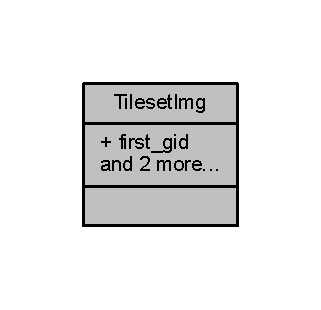
\includegraphics[width=154pt]{struct_tileset_img__coll__graph}
\end{center}
\end{figure}
\subsection*{Public Attributes}
\begin{DoxyCompactItemize}
\item 
\mbox{\Hypertarget{struct_tileset_img_a5cb5a67d6afd202da1aafd53e509167c}\label{struct_tileset_img_a5cb5a67d6afd202da1aafd53e509167c}} 
int \hyperlink{struct_tileset_img_a5cb5a67d6afd202da1aafd53e509167c}{first\+\_\+gid}
\begin{DoxyCompactList}\small\item\em number of the first tile in whole row \end{DoxyCompactList}\item 
\mbox{\Hypertarget{struct_tileset_img_a2cf02afb15fac885b30fd7d4d56374c1}\label{struct_tileset_img_a2cf02afb15fac885b30fd7d4d56374c1}} 
int \hyperlink{struct_tileset_img_a2cf02afb15fac885b30fd7d4d56374c1}{last\+\_\+gid}
\begin{DoxyCompactList}\small\item\em number of the last tile in whole row \end{DoxyCompactList}\item 
\mbox{\Hypertarget{struct_tileset_img_a9bd1b96e5ce27e6cb778d9fb96138883}\label{struct_tileset_img_a9bd1b96e5ce27e6cb778d9fb96138883}} 
int \hyperlink{struct_tileset_img_a9bd1b96e5ce27e6cb778d9fb96138883}{columns}
\begin{DoxyCompactList}\small\item\em number of columns that this tileset contains \end{DoxyCompactList}\end{DoxyCompactItemize}


\subsection{Detailed Description}
Contains information about tileset images. 

\begin{DoxyAuthor}{Author}
Vasily 
\end{DoxyAuthor}
\begin{DoxyVersion}{Version}
1.\+0 
\end{DoxyVersion}
\begin{DoxyDate}{Date}
June 2017 
\end{DoxyDate}


The documentation for this struct was generated from the following file\+:\begin{DoxyCompactItemize}
\item 
\hyperlink{_level_box_8h}{Level\+Box.\+h}\end{DoxyCompactItemize}

\hypertarget{class_timer}{}\section{Timer Class Reference}
\label{class_timer}\index{Timer@{Timer}}


Collaboration diagram for Timer\+:\nopagebreak
\begin{figure}[H]
\begin{center}
\leavevmode
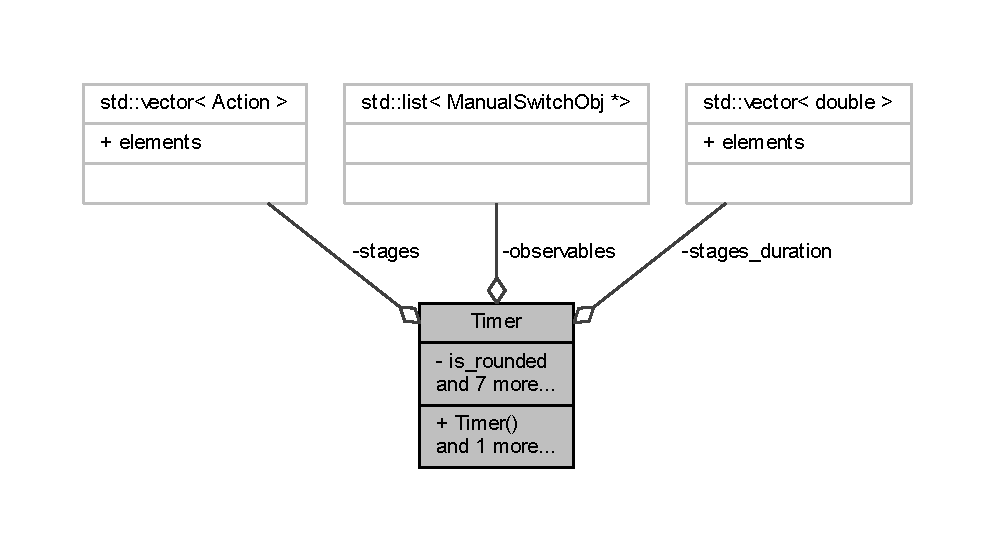
\includegraphics[width=160pt]{class_timer__coll__graph}
\end{center}
\end{figure}
\subsection*{Public Member Functions}
\begin{DoxyCompactItemize}
\item 
\mbox{\Hypertarget{class_timer_a0b2aa28140cd3a79edb0fbdafcbb9ee0}\label{class_timer_a0b2aa28140cd3a79edb0fbdafcbb9ee0}} 
{\bfseries Timer} (std\+::list$<$ \hyperlink{class_manual_switch_obj}{Manual\+Switch\+Obj} $\ast$$>$ \+\_\+observables, std\+::vector$<$ double $>$ \+\_\+stages\+\_\+duration, bool \+\_\+is\+\_\+rounded, std\+::vector$<$ Action $>$ \+\_\+stages)
\item 
\mbox{\Hypertarget{class_timer_a745ad59b5a46744cd871a1129a25d74f}\label{class_timer_a745ad59b5a46744cd871a1129a25d74f}} 
void {\bfseries update} ()
\end{DoxyCompactItemize}
\subsection*{Private Attributes}
\begin{DoxyCompactItemize}
\item 
\mbox{\Hypertarget{class_timer_acf215281063a8be431d810725a804224}\label{class_timer_acf215281063a8be431d810725a804224}} 
std\+::list$<$ \hyperlink{class_manual_switch_obj}{Manual\+Switch\+Obj} $\ast$ $>$ {\bfseries observables}
\item 
\mbox{\Hypertarget{class_timer_a77e0f14caf59087a0afa9e466b3b8c4b}\label{class_timer_a77e0f14caf59087a0afa9e466b3b8c4b}} 
std\+::vector$<$ double $>$ {\bfseries stages\+\_\+duration}
\item 
\mbox{\Hypertarget{class_timer_a8f8c7d41223e9976d4588ef212286fb5}\label{class_timer_a8f8c7d41223e9976d4588ef212286fb5}} 
std\+::vector$<$ Action $>$ {\bfseries stages}
\item 
\mbox{\Hypertarget{class_timer_ac397f8917b155e12401dd9ab793c91d9}\label{class_timer_ac397f8917b155e12401dd9ab793c91d9}} 
bool {\bfseries is\+\_\+rounded}
\item 
\mbox{\Hypertarget{class_timer_a6f1066d49764f5fc746f5fd669d95a9f}\label{class_timer_a6f1066d49764f5fc746f5fd669d95a9f}} 
bool {\bfseries is\+\_\+active}
\item 
\mbox{\Hypertarget{class_timer_aa410e9f94d1cdb79090fcf159f8f4d8c}\label{class_timer_aa410e9f94d1cdb79090fcf159f8f4d8c}} 
double {\bfseries time}
\item 
\mbox{\Hypertarget{class_timer_ae5b386341474f4cb8f11227e884250ab}\label{class_timer_ae5b386341474f4cb8f11227e884250ab}} 
int {\bfseries curr\+\_\+iter}
\item 
\mbox{\Hypertarget{class_timer_a34caee928e5a02b075496a74329abaeb}\label{class_timer_a34caee928e5a02b075496a74329abaeb}} 
int {\bfseries stage\+\_\+iter}
\item 
\mbox{\Hypertarget{class_timer_a196651dd936adea933d014145a9ae38e}\label{class_timer_a196651dd936adea933d014145a9ae38e}} 
std\+::chrono\+::seconds {\bfseries dts}
\item 
\mbox{\Hypertarget{class_timer_a1f7d523a49922d1d2bbfa2b49ebd4b38}\label{class_timer_a1f7d523a49922d1d2bbfa2b49ebd4b38}} 
std\+::chrono\+::time\+\_\+point$<$ std\+::chrono\+::system\+\_\+clock $>$ {\bfseries start}
\item 
\mbox{\Hypertarget{class_timer_abb300a4bdf620b8711d1e90980096291}\label{class_timer_abb300a4bdf620b8711d1e90980096291}} 
std\+::chrono\+::time\+\_\+point$<$ std\+::chrono\+::system\+\_\+clock $>$ {\bfseries end}
\item 
\mbox{\Hypertarget{class_timer_a331df3365dd6a3a6eb3382a9bb36e3cc}\label{class_timer_a331df3365dd6a3a6eb3382a9bb36e3cc}} 
std\+::chrono\+::duration$<$ double $>$ {\bfseries duration}
\end{DoxyCompactItemize}


The documentation for this class was generated from the following files\+:\begin{DoxyCompactItemize}
\item 
Timer.\+h\item 
Timer.\+cpp\end{DoxyCompactItemize}

\hypertarget{class_viewer}{}\section{Viewer Class Reference}
\label{class_viewer}\index{Viewer@{Viewer}}


Collaboration diagram for Viewer\+:\nopagebreak
\begin{figure}[H]
\begin{center}
\leavevmode
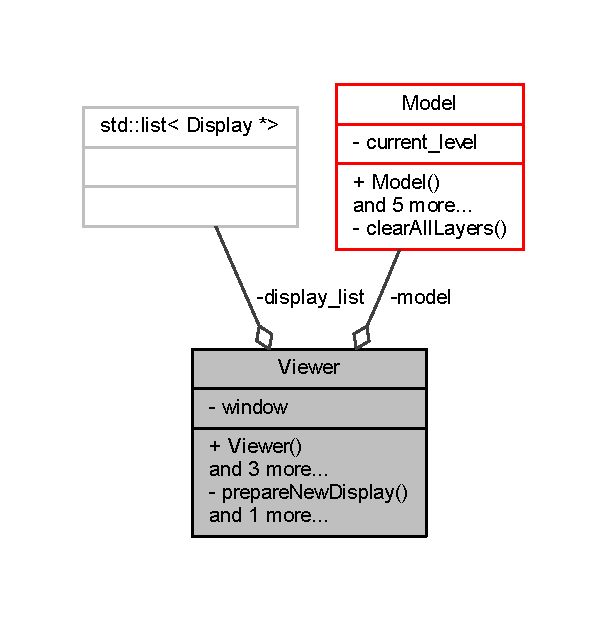
\includegraphics[width=192pt]{class_viewer__coll__graph}
\end{center}
\end{figure}
\subsection*{Public Member Functions}
\begin{DoxyCompactItemize}
\item 
\mbox{\Hypertarget{class_viewer_a767681a73f280357e6401f469c17ca4a}\label{class_viewer_a767681a73f280357e6401f469c17ca4a}} 
{\bfseries Viewer} (\hyperlink{class_model}{Model} $\ast$model)
\item 
\mbox{\Hypertarget{class_viewer_a7122ce13ef7b396ac8b7e471e4c82693}\label{class_viewer_a7122ce13ef7b396ac8b7e471e4c82693}} 
void {\bfseries update} ()
\item 
\mbox{\Hypertarget{class_viewer_aac14898275de71b0f0d43c11214852be}\label{class_viewer_aac14898275de71b0f0d43c11214852be}} 
void {\bfseries handle\+Viewer\+Event} (View\+Events)
\end{DoxyCompactItemize}
\subsection*{Private Member Functions}
\begin{DoxyCompactItemize}
\item 
\mbox{\Hypertarget{class_viewer_a2726818329086632b258a855b22e55ac}\label{class_viewer_a2726818329086632b258a855b22e55ac}} 
void {\bfseries prepare\+New\+Display} ()
\item 
\mbox{\Hypertarget{class_viewer_a6ee06f2f80d48076c42208250c017663}\label{class_viewer_a6ee06f2f80d48076c42208250c017663}} 
void {\bfseries delete\+Display} ()
\end{DoxyCompactItemize}
\subsection*{Private Attributes}
\begin{DoxyCompactItemize}
\item 
\mbox{\Hypertarget{class_viewer_a974fa8b6e46d1e09e334da06b769ab6b}\label{class_viewer_a974fa8b6e46d1e09e334da06b769ab6b}} 
\hyperlink{class_model}{Model} $\ast$ {\bfseries model}
\item 
\mbox{\Hypertarget{class_viewer_ae144a159f8ffcfd94e355cdab921b8d3}\label{class_viewer_ae144a159f8ffcfd94e355cdab921b8d3}} 
sf\+::\+Render\+Window $\ast$ {\bfseries window}
\item 
\mbox{\Hypertarget{class_viewer_a3f38d8aec27298408b8e5856a7ef2995}\label{class_viewer_a3f38d8aec27298408b8e5856a7ef2995}} 
std\+::list$<$ \hyperlink{class_display}{Display} $\ast$ $>$ {\bfseries display\+\_\+list}
\end{DoxyCompactItemize}


The documentation for this class was generated from the following files\+:\begin{DoxyCompactItemize}
\item 
Viewer.\+h\item 
Viewer.\+cpp\end{DoxyCompactItemize}

\hypertarget{class_visible_sensor}{}\section{Visible\+Sensor Class Reference}
\label{class_visible_sensor}\index{Visible\+Sensor@{Visible\+Sensor}}


Collaboration diagram for Visible\+Sensor\+:\nopagebreak
\begin{figure}[H]
\begin{center}
\leavevmode
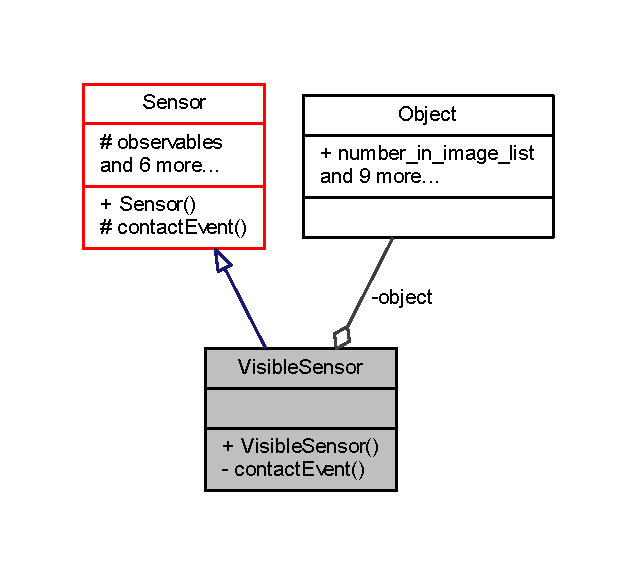
\includegraphics[width=306pt]{class_visible_sensor__coll__graph}
\end{center}
\end{figure}
\subsection*{Public Member Functions}
\begin{DoxyCompactItemize}
\item 
\mbox{\Hypertarget{class_visible_sensor_a45c102db9ef942dcb5bfc5dba9030add}\label{class_visible_sensor_a45c102db9ef942dcb5bfc5dba9030add}} 
{\bfseries Visible\+Sensor} (std\+::list$<$ \hyperlink{class_manual_switch_obj}{Manual\+Switch\+Obj} $\ast$$>$ \+\_\+observables, bool \+\_\+repeat\+\_\+allowed, bool is\+\_\+keeping, b2\+Body $\ast$\+\_\+body, \hyperlink{class_object}{Object} $\ast$\+\_\+object, std\+::vector$<$ Action $>$ \+\_\+stages)
\end{DoxyCompactItemize}
\subsection*{Private Member Functions}
\begin{DoxyCompactItemize}
\item 
void \hyperlink{class_visible_sensor_a63bcb9da7556a6356cca3b08f7808bd8}{contact\+Event} (b2\+Contact $\ast$, bool)
\begin{DoxyCompactList}\small\item\em Define object reaction to the collision in box2d world. \end{DoxyCompactList}\end{DoxyCompactItemize}
\subsection*{Private Attributes}
\begin{DoxyCompactItemize}
\item 
\mbox{\Hypertarget{class_visible_sensor_a933e07d2186c63f9333778a213dd0cd5}\label{class_visible_sensor_a933e07d2186c63f9333778a213dd0cd5}} 
\hyperlink{class_object}{Object} $\ast$ {\bfseries object}
\end{DoxyCompactItemize}
\subsection*{Additional Inherited Members}


\subsection{Member Function Documentation}
\mbox{\Hypertarget{class_visible_sensor_a63bcb9da7556a6356cca3b08f7808bd8}\label{class_visible_sensor_a63bcb9da7556a6356cca3b08f7808bd8}} 
\index{Visible\+Sensor@{Visible\+Sensor}!contact\+Event@{contact\+Event}}
\index{contact\+Event@{contact\+Event}!Visible\+Sensor@{Visible\+Sensor}}
\subsubsection{\texorpdfstring{contact\+Event()}{contactEvent()}}
{\footnotesize\ttfamily void Visible\+Sensor\+::contact\+Event (\begin{DoxyParamCaption}\item[{b2\+Contact $\ast$}]{contact,  }\item[{bool}]{is\+Begin }\end{DoxyParamCaption})\hspace{0.3cm}{\ttfamily [private]}, {\ttfamily [virtual]}}



Define object reaction to the collision in box2d world. 


\begin{DoxyParams}{Parameters}
{\em contact} & pointer to box2d b2\+Contact class \\
\hline
{\em is\+Begin} & \textquotesingle{}false\textquotesingle{} -\/ end of the collision; \textquotesingle{}true\textquotesingle{} -\/ start of the collision \\
\hline
\end{DoxyParams}


Reimplemented from \hyperlink{class_sensor_a08bfa36c84277677f3bd5fb14127fca7}{Sensor}.



The documentation for this class was generated from the following files\+:\begin{DoxyCompactItemize}
\item 
Visible\+Sensor.\+h\item 
Visible\+Sensor.\+cpp\end{DoxyCompactItemize}

\hypertarget{class_win_singleton}{}\section{Win\+Singleton Class Reference}
\label{class_win_singleton}\index{Win\+Singleton@{Win\+Singleton}}


Collaboration diagram for Win\+Singleton\+:\nopagebreak
\begin{figure}[H]
\begin{center}
\leavevmode
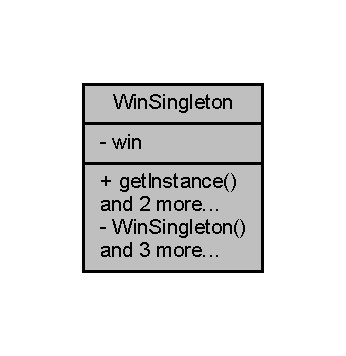
\includegraphics[width=166pt]{class_win_singleton__coll__graph}
\end{center}
\end{figure}
\subsection*{Static Public Member Functions}
\begin{DoxyCompactItemize}
\item 
\mbox{\Hypertarget{class_win_singleton_a82935bb60c8e4bb14350ac45813b33ca}\label{class_win_singleton_a82935bb60c8e4bb14350ac45813b33ca}} 
static sf\+::\+Render\+Window $\ast$ {\bfseries get\+Instance} ()
\item 
\mbox{\Hypertarget{class_win_singleton_a58684b65df9dadcdc798faba86aeb0b6}\label{class_win_singleton_a58684b65df9dadcdc798faba86aeb0b6}} 
static void {\bfseries to\+Full\+Screen} ()
\item 
\mbox{\Hypertarget{class_win_singleton_abba34d9cbdf6a9ff14da654b2b88aba3}\label{class_win_singleton_abba34d9cbdf6a9ff14da654b2b88aba3}} 
static void {\bfseries to\+Window} ()
\end{DoxyCompactItemize}
\subsection*{Private Member Functions}
\begin{DoxyCompactItemize}
\item 
\mbox{\Hypertarget{class_win_singleton_a8afac0ce148375d8e3d953e881891b53}\label{class_win_singleton_a8afac0ce148375d8e3d953e881891b53}} 
{\bfseries Win\+Singleton} (\hyperlink{class_win_singleton}{Win\+Singleton} const \&)=delete
\item 
\mbox{\Hypertarget{class_win_singleton_a8585d53112439fe088484c9cbf8a26b6}\label{class_win_singleton_a8585d53112439fe088484c9cbf8a26b6}} 
\hyperlink{class_win_singleton}{Win\+Singleton} \& {\bfseries operator=} (\hyperlink{class_win_singleton}{Win\+Singleton} const \&)=delete
\end{DoxyCompactItemize}
\subsection*{Static Private Attributes}
\begin{DoxyCompactItemize}
\item 
\mbox{\Hypertarget{class_win_singleton_ad2469dc3ef435d5739cda832be2b556f}\label{class_win_singleton_ad2469dc3ef435d5739cda832be2b556f}} 
static sf\+::\+Render\+Window $\ast$ {\bfseries win} = nullptr
\end{DoxyCompactItemize}


The documentation for this class was generated from the following files\+:\begin{DoxyCompactItemize}
\item 
Win\+Singleton.\+h\item 
Win\+Singleton.\+cpp\end{DoxyCompactItemize}

\chapter{File Documentation}
\hypertarget{_advanced_display_8h}{}\section{Advanced\+Display.\+h File Reference}
\label{_advanced_display_8h}\index{Advanced\+Display.\+h@{Advanced\+Display.\+h}}
{\ttfamily \#include \char`\"{}Display.\+h\char`\"{}}\newline
Include dependency graph for Advanced\+Display.\+h\+:
\nopagebreak
\begin{figure}[H]
\begin{center}
\leavevmode
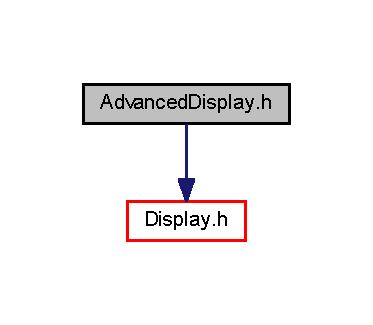
\includegraphics[width=179pt]{_advanced_display_8h__incl}
\end{center}
\end{figure}
This graph shows which files directly or indirectly include this file\+:
\nopagebreak
\begin{figure}[H]
\begin{center}
\leavevmode
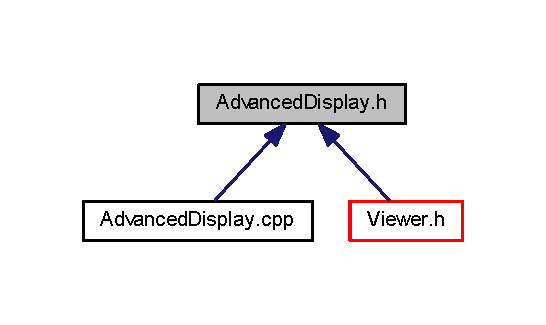
\includegraphics[width=262pt]{_advanced_display_8h__dep__incl}
\end{center}
\end{figure}
\subsection*{Classes}
\begin{DoxyCompactItemize}
\item 
class \hyperlink{class_advanced_display}{Advanced\+Display}
\end{DoxyCompactItemize}

\hypertarget{_auxiliary_layer_8h}{}\section{Auxiliary\+Layer.\+h File Reference}
\label{_auxiliary_layer_8h}\index{Auxiliary\+Layer.\+h@{Auxiliary\+Layer.\+h}}
{\ttfamily \#include \char`\"{}Layer.\+h\char`\"{}}\newline
Include dependency graph for Auxiliary\+Layer.\+h\+:\nopagebreak
\begin{figure}[H]
\begin{center}
\leavevmode
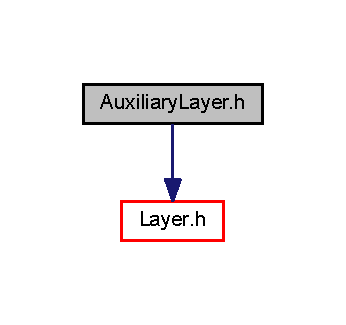
\includegraphics[width=166pt]{_auxiliary_layer_8h__incl}
\end{center}
\end{figure}
This graph shows which files directly or indirectly include this file\+:\nopagebreak
\begin{figure}[H]
\begin{center}
\leavevmode
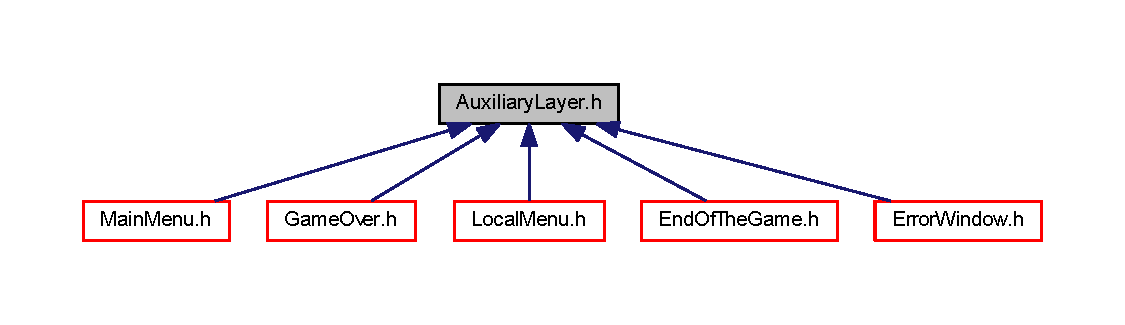
\includegraphics[width=350pt]{_auxiliary_layer_8h__dep__incl}
\end{center}
\end{figure}
\subsection*{Classes}
\begin{DoxyCompactItemize}
\item 
class \hyperlink{class_auxiliary_layer}{Auxiliary\+Layer}
\begin{DoxyCompactList}\small\item\em Superstructure class for built-\/in \hyperlink{class_layer}{Layer} classes. \end{DoxyCompactList}\end{DoxyCompactItemize}

\hypertarget{_bonus_8h}{}\section{Bonus.\+h File Reference}
\label{_bonus_8h}\index{Bonus.\+h@{Bonus.\+h}}
{\ttfamily \#include \char`\"{}Contact\+Object.\+h\char`\"{}}\newline
{\ttfamily \#include \char`\"{}Player.\+h\char`\"{}}\newline
{\ttfamily \#include $<$chrono$>$}\newline
Include dependency graph for Bonus.\+h\+:
\nopagebreak
\begin{figure}[H]
\begin{center}
\leavevmode
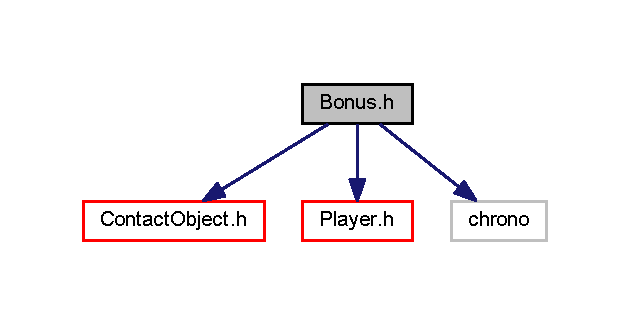
\includegraphics[width=303pt]{_bonus_8h__incl}
\end{center}
\end{figure}
This graph shows which files directly or indirectly include this file\+:
\nopagebreak
\begin{figure}[H]
\begin{center}
\leavevmode
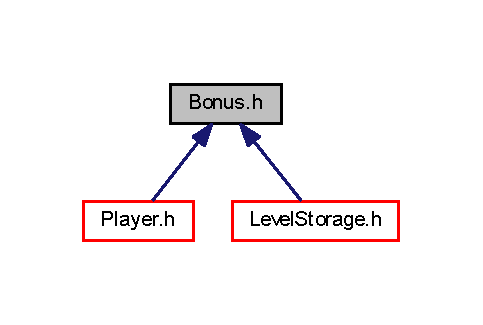
\includegraphics[width=323pt]{_bonus_8h__dep__incl}
\end{center}
\end{figure}
\subsection*{Classes}
\begin{DoxyCompactItemize}
\item 
class \hyperlink{class_bonus}{Bonus}
\end{DoxyCompactItemize}

\hypertarget{_contact_listener_8h}{}\section{Contact\+Listener.\+h File Reference}
\label{_contact_listener_8h}\index{Contact\+Listener.\+h@{Contact\+Listener.\+h}}
{\ttfamily \#include \char`\"{}Non\+Static\+Obj.\+h\char`\"{}}\newline
{\ttfamily \#include $<$list$>$}\newline
Include dependency graph for Contact\+Listener.\+h\+:
\nopagebreak
\begin{figure}[H]
\begin{center}
\leavevmode
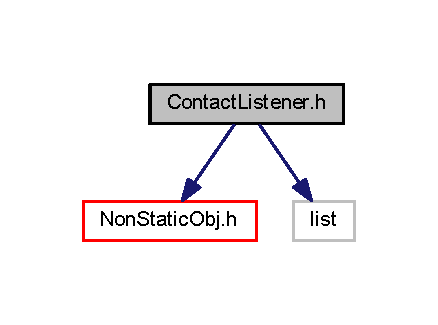
\includegraphics[width=210pt]{_contact_listener_8h__incl}
\end{center}
\end{figure}
This graph shows which files directly or indirectly include this file\+:
\nopagebreak
\begin{figure}[H]
\begin{center}
\leavevmode
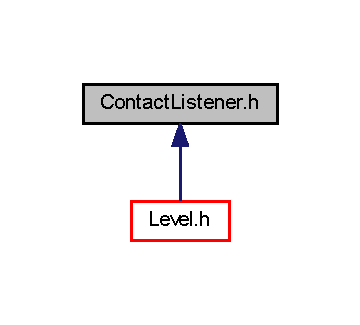
\includegraphics[width=173pt]{_contact_listener_8h__dep__incl}
\end{center}
\end{figure}
\subsection*{Classes}
\begin{DoxyCompactItemize}
\item 
class \hyperlink{class_my_contact_listener}{My\+Contact\+Listener}
\begin{DoxyCompactList}\small\item\em Override for standart box2d Contact\+Listener. \end{DoxyCompactList}\end{DoxyCompactItemize}

\hypertarget{_contact_object_8h}{}\section{Contact\+Object.\+h File Reference}
\label{_contact_object_8h}\index{Contact\+Object.\+h@{Contact\+Object.\+h}}
{\ttfamily \#include \char`\"{}Box2\+D\textbackslash{}\+Box2\+D.\+h\char`\"{}}\newline
Include dependency graph for Contact\+Object.\+h\+:\nopagebreak
\begin{figure}[H]
\begin{center}
\leavevmode
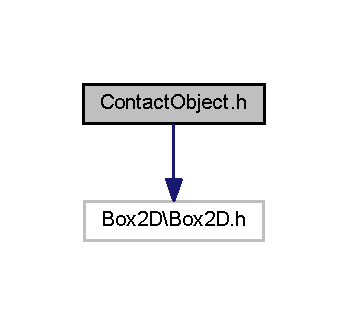
\includegraphics[width=167pt]{_contact_object_8h__incl}
\end{center}
\end{figure}
This graph shows which files directly or indirectly include this file\+:\nopagebreak
\begin{figure}[H]
\begin{center}
\leavevmode
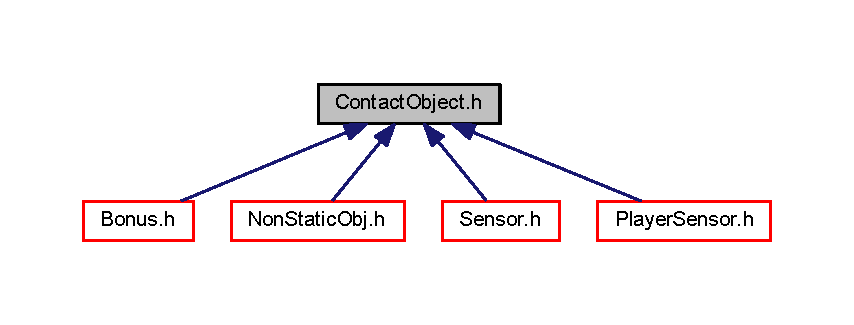
\includegraphics[width=350pt]{_contact_object_8h__dep__incl}
\end{center}
\end{figure}
\subsection*{Classes}
\begin{DoxyCompactItemize}
\item 
class \hyperlink{class_contact_object}{Contact\+Object}
\begin{DoxyCompactList}\small\item\em Interface for an object which can collide with another in box2d world. \end{DoxyCompactList}\end{DoxyCompactItemize}
\subsection*{Enumerations}
\begin{DoxyCompactItemize}
\item 
enum \hyperlink{_contact_object_8h_a684af1cf542217fe5ea2859096b5fa51}{Entity\+Category} \{ \newline
\hyperlink{_contact_object_8h_a684af1cf542217fe5ea2859096b5fa51ae95dcc9c84efdb46a30b0e2e6a477ce3}{S\+T\+R\+O\+N\+G\+\_\+\+P\+L\+A\+Y\+ER} = 0x0001, 
\hyperlink{_contact_object_8h_a684af1cf542217fe5ea2859096b5fa51a92b136a57e2a1a3a80292e811ac53ad6}{D\+E\+X\+T\+E\+R\+O\+U\+S\+\_\+\+P\+L\+A\+Y\+ER} = 0x0002, 
\hyperlink{_contact_object_8h_a684af1cf542217fe5ea2859096b5fa51a137858cdb6aa2ed51a2389be72b9552c}{D\+A\+N\+G\+E\+RS} = 0x0004, 
\hyperlink{_contact_object_8h_a684af1cf542217fe5ea2859096b5fa51a4af5fe82e7a2c651d3a04f3d5aa2bef7}{O\+T\+H\+E\+RS} = 0x0008, 
\newline
\hyperlink{_contact_object_8h_a684af1cf542217fe5ea2859096b5fa51a640a1773614b51214db3c0e77219ce1d}{B\+O\+N\+U\+S\+ES} = 0x0010
 \}\begin{DoxyCompactList}\small\item\em Bitmask for objects, participating box2d collision. \end{DoxyCompactList}
\item 
enum \hyperlink{_contact_object_8h_a51b6f30553a2b7a2c81727faaacd1613}{Entity\+Group} \{ \newline
\hyperlink{_contact_object_8h_a51b6f30553a2b7a2c81727faaacd1613a773fa1db63a772499c5951ea9f7a781f}{M\+A\+S\+K\+\_\+\+P\+L\+A\+Y\+E\+RS} = S\+T\+R\+O\+N\+G\+\_\+\+P\+L\+A\+Y\+ER $\vert$ D\+E\+X\+T\+E\+R\+O\+U\+S\+\_\+\+P\+L\+A\+Y\+ER, 
\hyperlink{_contact_object_8h_a51b6f30553a2b7a2c81727faaacd1613ae4a6082b7586ae5a73f21757ff2c11a4}{M\+A\+S\+K\+\_\+\+P\+L\+A\+Y\+ER} = $\sim$\+M\+A\+S\+K\+\_\+\+P\+L\+A\+Y\+E\+RS, 
\hyperlink{_contact_object_8h_a51b6f30553a2b7a2c81727faaacd1613a405be940b75cd32230f86e7260e0abf2}{M\+A\+S\+K\+\_\+\+D\+A\+N\+G\+E\+RS} = M\+A\+S\+K\+\_\+\+P\+L\+A\+Y\+E\+RS, 
\hyperlink{_contact_object_8h_a51b6f30553a2b7a2c81727faaacd1613aaa5264382487de8648462a49e203aaf5}{M\+A\+S\+K\+\_\+\+O\+T\+H\+E\+RS} = M\+A\+S\+K\+\_\+\+P\+L\+A\+Y\+E\+RS $\vert$ O\+T\+H\+E\+RS, 
\newline
\hyperlink{_contact_object_8h_a51b6f30553a2b7a2c81727faaacd1613a5622b177bb0b248e766b36c26b5d420b}{M\+A\+S\+K\+\_\+\+B\+O\+N\+U\+S\+ES} = M\+A\+S\+K\+\_\+\+P\+L\+A\+Y\+E\+RS
 \}\begin{DoxyCompactList}\small\item\em Bitmask-\/rule for box2d collision. \end{DoxyCompactList}
\end{DoxyCompactItemize}


\subsection{Enumeration Type Documentation}
\mbox{\Hypertarget{_contact_object_8h_a684af1cf542217fe5ea2859096b5fa51}\label{_contact_object_8h_a684af1cf542217fe5ea2859096b5fa51}} 
\index{Contact\+Object.\+h@{Contact\+Object.\+h}!Entity\+Category@{Entity\+Category}}
\index{Entity\+Category@{Entity\+Category}!Contact\+Object.\+h@{Contact\+Object.\+h}}
\subsubsection{\texorpdfstring{Entity\+Category}{EntityCategory}}
{\footnotesize\ttfamily enum \hyperlink{_contact_object_8h_a684af1cf542217fe5ea2859096b5fa51}{Entity\+Category}}



Bitmask for objects, participating box2d collision. 

\begin{DoxyEnumFields}{Enumerator}
\raisebox{\heightof{T}}[0pt][0pt]{\index{S\+T\+R\+O\+N\+G\+\_\+\+P\+L\+A\+Y\+ER@{S\+T\+R\+O\+N\+G\+\_\+\+P\+L\+A\+Y\+ER}!Contact\+Object.\+h@{Contact\+Object.\+h}}\index{Contact\+Object.\+h@{Contact\+Object.\+h}!S\+T\+R\+O\+N\+G\+\_\+\+P\+L\+A\+Y\+ER@{S\+T\+R\+O\+N\+G\+\_\+\+P\+L\+A\+Y\+ER}}}\mbox{\Hypertarget{_contact_object_8h_a684af1cf542217fe5ea2859096b5fa51ae95dcc9c84efdb46a30b0e2e6a477ce3}\label{_contact_object_8h_a684af1cf542217fe5ea2859096b5fa51ae95dcc9c84efdb46a30b0e2e6a477ce3}} 
S\+T\+R\+O\+N\+G\+\_\+\+P\+L\+A\+Y\+ER&Mask for strong player. \\
\hline

\raisebox{\heightof{T}}[0pt][0pt]{\index{D\+E\+X\+T\+E\+R\+O\+U\+S\+\_\+\+P\+L\+A\+Y\+ER@{D\+E\+X\+T\+E\+R\+O\+U\+S\+\_\+\+P\+L\+A\+Y\+ER}!Contact\+Object.\+h@{Contact\+Object.\+h}}\index{Contact\+Object.\+h@{Contact\+Object.\+h}!D\+E\+X\+T\+E\+R\+O\+U\+S\+\_\+\+P\+L\+A\+Y\+ER@{D\+E\+X\+T\+E\+R\+O\+U\+S\+\_\+\+P\+L\+A\+Y\+ER}}}\mbox{\Hypertarget{_contact_object_8h_a684af1cf542217fe5ea2859096b5fa51a92b136a57e2a1a3a80292e811ac53ad6}\label{_contact_object_8h_a684af1cf542217fe5ea2859096b5fa51a92b136a57e2a1a3a80292e811ac53ad6}} 
D\+E\+X\+T\+E\+R\+O\+U\+S\+\_\+\+P\+L\+A\+Y\+ER&Mask for dexterous player. \\
\hline

\raisebox{\heightof{T}}[0pt][0pt]{\index{D\+A\+N\+G\+E\+RS@{D\+A\+N\+G\+E\+RS}!Contact\+Object.\+h@{Contact\+Object.\+h}}\index{Contact\+Object.\+h@{Contact\+Object.\+h}!D\+A\+N\+G\+E\+RS@{D\+A\+N\+G\+E\+RS}}}\mbox{\Hypertarget{_contact_object_8h_a684af1cf542217fe5ea2859096b5fa51a137858cdb6aa2ed51a2389be72b9552c}\label{_contact_object_8h_a684af1cf542217fe5ea2859096b5fa51a137858cdb6aa2ed51a2389be72b9552c}} 
D\+A\+N\+G\+E\+RS&Mask for kinematic danger objects. \\
\hline

\raisebox{\heightof{T}}[0pt][0pt]{\index{O\+T\+H\+E\+RS@{O\+T\+H\+E\+RS}!Contact\+Object.\+h@{Contact\+Object.\+h}}\index{Contact\+Object.\+h@{Contact\+Object.\+h}!O\+T\+H\+E\+RS@{O\+T\+H\+E\+RS}}}\mbox{\Hypertarget{_contact_object_8h_a684af1cf542217fe5ea2859096b5fa51a4af5fe82e7a2c651d3a04f3d5aa2bef7}\label{_contact_object_8h_a684af1cf542217fe5ea2859096b5fa51a4af5fe82e7a2c651d3a04f3d5aa2bef7}} 
O\+T\+H\+E\+RS&Mask for all other objects. \\
\hline

\raisebox{\heightof{T}}[0pt][0pt]{\index{B\+O\+N\+U\+S\+ES@{B\+O\+N\+U\+S\+ES}!Contact\+Object.\+h@{Contact\+Object.\+h}}\index{Contact\+Object.\+h@{Contact\+Object.\+h}!B\+O\+N\+U\+S\+ES@{B\+O\+N\+U\+S\+ES}}}\mbox{\Hypertarget{_contact_object_8h_a684af1cf542217fe5ea2859096b5fa51a640a1773614b51214db3c0e77219ce1d}\label{_contact_object_8h_a684af1cf542217fe5ea2859096b5fa51a640a1773614b51214db3c0e77219ce1d}} 
B\+O\+N\+U\+S\+ES&Mask for bonus objects. \\
\hline

\end{DoxyEnumFields}
\mbox{\Hypertarget{_contact_object_8h_a51b6f30553a2b7a2c81727faaacd1613}\label{_contact_object_8h_a51b6f30553a2b7a2c81727faaacd1613}} 
\index{Contact\+Object.\+h@{Contact\+Object.\+h}!Entity\+Group@{Entity\+Group}}
\index{Entity\+Group@{Entity\+Group}!Contact\+Object.\+h@{Contact\+Object.\+h}}
\subsubsection{\texorpdfstring{Entity\+Group}{EntityGroup}}
{\footnotesize\ttfamily enum \hyperlink{_contact_object_8h_a51b6f30553a2b7a2c81727faaacd1613}{Entity\+Group}}



Bitmask-\/rule for box2d collision. 

\begin{DoxyEnumFields}{Enumerator}
\raisebox{\heightof{T}}[0pt][0pt]{\index{M\+A\+S\+K\+\_\+\+P\+L\+A\+Y\+E\+RS@{M\+A\+S\+K\+\_\+\+P\+L\+A\+Y\+E\+RS}!Contact\+Object.\+h@{Contact\+Object.\+h}}\index{Contact\+Object.\+h@{Contact\+Object.\+h}!M\+A\+S\+K\+\_\+\+P\+L\+A\+Y\+E\+RS@{M\+A\+S\+K\+\_\+\+P\+L\+A\+Y\+E\+RS}}}\mbox{\Hypertarget{_contact_object_8h_a51b6f30553a2b7a2c81727faaacd1613a773fa1db63a772499c5951ea9f7a781f}\label{_contact_object_8h_a51b6f30553a2b7a2c81727faaacd1613a773fa1db63a772499c5951ea9f7a781f}} 
M\+A\+S\+K\+\_\+\+P\+L\+A\+Y\+E\+RS&Mask for players. \\
\hline

\raisebox{\heightof{T}}[0pt][0pt]{\index{M\+A\+S\+K\+\_\+\+P\+L\+A\+Y\+ER@{M\+A\+S\+K\+\_\+\+P\+L\+A\+Y\+ER}!Contact\+Object.\+h@{Contact\+Object.\+h}}\index{Contact\+Object.\+h@{Contact\+Object.\+h}!M\+A\+S\+K\+\_\+\+P\+L\+A\+Y\+ER@{M\+A\+S\+K\+\_\+\+P\+L\+A\+Y\+ER}}}\mbox{\Hypertarget{_contact_object_8h_a51b6f30553a2b7a2c81727faaacd1613ae4a6082b7586ae5a73f21757ff2c11a4}\label{_contact_object_8h_a51b6f30553a2b7a2c81727faaacd1613ae4a6082b7586ae5a73f21757ff2c11a4}} 
M\+A\+S\+K\+\_\+\+P\+L\+A\+Y\+ER&Rule for players. \\
\hline

\raisebox{\heightof{T}}[0pt][0pt]{\index{M\+A\+S\+K\+\_\+\+D\+A\+N\+G\+E\+RS@{M\+A\+S\+K\+\_\+\+D\+A\+N\+G\+E\+RS}!Contact\+Object.\+h@{Contact\+Object.\+h}}\index{Contact\+Object.\+h@{Contact\+Object.\+h}!M\+A\+S\+K\+\_\+\+D\+A\+N\+G\+E\+RS@{M\+A\+S\+K\+\_\+\+D\+A\+N\+G\+E\+RS}}}\mbox{\Hypertarget{_contact_object_8h_a51b6f30553a2b7a2c81727faaacd1613a405be940b75cd32230f86e7260e0abf2}\label{_contact_object_8h_a51b6f30553a2b7a2c81727faaacd1613a405be940b75cd32230f86e7260e0abf2}} 
M\+A\+S\+K\+\_\+\+D\+A\+N\+G\+E\+RS&Rule for kinematic danger objects. \\
\hline

\raisebox{\heightof{T}}[0pt][0pt]{\index{M\+A\+S\+K\+\_\+\+O\+T\+H\+E\+RS@{M\+A\+S\+K\+\_\+\+O\+T\+H\+E\+RS}!Contact\+Object.\+h@{Contact\+Object.\+h}}\index{Contact\+Object.\+h@{Contact\+Object.\+h}!M\+A\+S\+K\+\_\+\+O\+T\+H\+E\+RS@{M\+A\+S\+K\+\_\+\+O\+T\+H\+E\+RS}}}\mbox{\Hypertarget{_contact_object_8h_a51b6f30553a2b7a2c81727faaacd1613aaa5264382487de8648462a49e203aaf5}\label{_contact_object_8h_a51b6f30553a2b7a2c81727faaacd1613aaa5264382487de8648462a49e203aaf5}} 
M\+A\+S\+K\+\_\+\+O\+T\+H\+E\+RS&Rule for all other objects. \\
\hline

\raisebox{\heightof{T}}[0pt][0pt]{\index{M\+A\+S\+K\+\_\+\+B\+O\+N\+U\+S\+ES@{M\+A\+S\+K\+\_\+\+B\+O\+N\+U\+S\+ES}!Contact\+Object.\+h@{Contact\+Object.\+h}}\index{Contact\+Object.\+h@{Contact\+Object.\+h}!M\+A\+S\+K\+\_\+\+B\+O\+N\+U\+S\+ES@{M\+A\+S\+K\+\_\+\+B\+O\+N\+U\+S\+ES}}}\mbox{\Hypertarget{_contact_object_8h_a51b6f30553a2b7a2c81727faaacd1613a5622b177bb0b248e766b36c26b5d420b}\label{_contact_object_8h_a51b6f30553a2b7a2c81727faaacd1613a5622b177bb0b248e766b36c26b5d420b}} 
M\+A\+S\+K\+\_\+\+B\+O\+N\+U\+S\+ES&Rule for bonus objects. \\
\hline

\end{DoxyEnumFields}

\hypertarget{_controller_8h}{}\section{Controller.\+h File Reference}
\label{_controller_8h}\index{Controller.\+h@{Controller.\+h}}
{\ttfamily \#include \char`\"{}Viewer.\+h\char`\"{}}\newline
Include dependency graph for Controller.\+h\+:\nopagebreak
\begin{figure}[H]
\begin{center}
\leavevmode
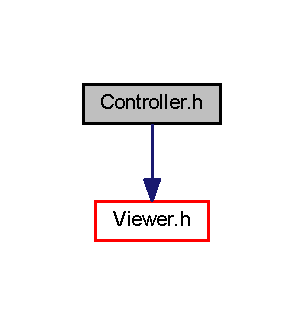
\includegraphics[width=146pt]{_controller_8h__incl}
\end{center}
\end{figure}
\subsection*{Classes}
\begin{DoxyCompactItemize}
\item 
class \hyperlink{class_controller}{Controller}
\begin{DoxyCompactList}\small\item\em Operating element in M\+VC structure. \end{DoxyCompactList}\end{DoxyCompactItemize}

\hypertarget{_danger_object_8h}{}\section{Danger\+Object.\+h File Reference}
\label{_danger_object_8h}\index{Danger\+Object.\+h@{Danger\+Object.\+h}}
{\ttfamily \#include $<$vector$>$}\newline
{\ttfamily \#include $<$list$>$}\newline
{\ttfamily \#include $<$chrono$>$}\newline
{\ttfamily \#include \char`\"{}Player.\+h\char`\"{}}\newline
Include dependency graph for Danger\+Object.\+h\+:
\nopagebreak
\begin{figure}[H]
\begin{center}
\leavevmode
\includegraphics[width=306pt]{_danger_object_8h__incl}
\end{center}
\end{figure}
This graph shows which files directly or indirectly include this file\+:
\nopagebreak
\begin{figure}[H]
\begin{center}
\leavevmode
\includegraphics[width=164pt]{_danger_object_8h__dep__incl}
\end{center}
\end{figure}
\subsection*{Classes}
\begin{DoxyCompactItemize}
\item 
class \hyperlink{class_danger_object}{Danger\+Object}
\begin{DoxyCompactList}\small\item\em Danger entity that can be assigned to the platform. \end{DoxyCompactList}\end{DoxyCompactItemize}

\hypertarget{_dexterous_player_8h}{}\section{Dexterous\+Player.\+h File Reference}
\label{_dexterous_player_8h}\index{Dexterous\+Player.\+h@{Dexterous\+Player.\+h}}
{\ttfamily \#include \char`\"{}Player.\+h\char`\"{}}\newline
Include dependency graph for Dexterous\+Player.\+h\+:
\nopagebreak
\begin{figure}[H]
\begin{center}
\leavevmode
\includegraphics[width=177pt]{_dexterous_player_8h__incl}
\end{center}
\end{figure}
This graph shows which files directly or indirectly include this file\+:
\nopagebreak
\begin{figure}[H]
\begin{center}
\leavevmode
\includegraphics[width=177pt]{_dexterous_player_8h__dep__incl}
\end{center}
\end{figure}
\subsection*{Classes}
\begin{DoxyCompactItemize}
\item 
class \hyperlink{class_dexterous_player}{Dexterous\+Player}
\begin{DoxyCompactList}\small\item\em Contains information about dexterous characret. \end{DoxyCompactList}\end{DoxyCompactItemize}

\hypertarget{_display_8h}{}\section{Display.\+h File Reference}
\label{_display_8h}\index{Display.\+h@{Display.\+h}}
{\ttfamily \#include $<$S\+F\+M\+L/\+Graphics.\+hpp$>$}\newline
{\ttfamily \#include \char`\"{}Layer.\+h\char`\"{}}\newline
Include dependency graph for Display.\+h\+:\nopagebreak
\begin{figure}[H]
\begin{center}
\leavevmode
\includegraphics[width=252pt]{_display_8h__incl}
\end{center}
\end{figure}
This graph shows which files directly or indirectly include this file\+:\nopagebreak
\begin{figure}[H]
\begin{center}
\leavevmode
\includegraphics[width=179pt]{_display_8h__dep__incl}
\end{center}
\end{figure}
\subsection*{Classes}
\begin{DoxyCompactItemize}
\item 
class \hyperlink{class_display}{Display}
\begin{DoxyCompactList}\small\item\em Provides a display for \hyperlink{class_layer}{Layer} information. \end{DoxyCompactList}\end{DoxyCompactItemize}

\hypertarget{_end_of_the_game_8h}{}\section{End\+Of\+The\+Game.\+h File Reference}
\label{_end_of_the_game_8h}\index{End\+Of\+The\+Game.\+h@{End\+Of\+The\+Game.\+h}}
{\ttfamily \#include \char`\"{}Auxiliary\+Layer.\+h\char`\"{}}\newline
Include dependency graph for End\+Of\+The\+Game.\+h\+:
\nopagebreak
\begin{figure}[H]
\begin{center}
\leavevmode
\includegraphics[width=174pt]{_end_of_the_game_8h__incl}
\end{center}
\end{figure}
This graph shows which files directly or indirectly include this file\+:
\nopagebreak
\begin{figure}[H]
\begin{center}
\leavevmode
\includegraphics[width=174pt]{_end_of_the_game_8h__dep__incl}
\end{center}
\end{figure}
\subsection*{Classes}
\begin{DoxyCompactItemize}
\item 
class \hyperlink{class_end_of_the_game}{End\+Of\+The\+Game}
\begin{DoxyCompactList}\small\item\em \char`\"{}\+The End\char`\"{} screen \end{DoxyCompactList}\end{DoxyCompactItemize}

\hypertarget{_error_window_8h}{}\section{Error\+Window.\+h File Reference}
\label{_error_window_8h}\index{Error\+Window.\+h@{Error\+Window.\+h}}
{\ttfamily \#include \char`\"{}Auxiliary\+Layer.\+h\char`\"{}}\newline
Include dependency graph for Error\+Window.\+h\+:\nopagebreak
\begin{figure}[H]
\begin{center}
\leavevmode
\includegraphics[width=166pt]{_error_window_8h__incl}
\end{center}
\end{figure}
This graph shows which files directly or indirectly include this file\+:\nopagebreak
\begin{figure}[H]
\begin{center}
\leavevmode
\includegraphics[width=160pt]{_error_window_8h__dep__incl}
\end{center}
\end{figure}
\subsection*{Classes}
\begin{DoxyCompactItemize}
\item 
class \hyperlink{class_error_window}{Error\+Window}
\begin{DoxyCompactList}\small\item\em \char`\"{}\+The Error\char`\"{} screen \end{DoxyCompactList}\end{DoxyCompactItemize}

\hypertarget{_events_8h}{}\section{Events.\+h File Reference}
\label{_events_8h}\index{Events.\+h@{Events.\+h}}
This graph shows which files directly or indirectly include this file\+:\nopagebreak
\begin{figure}[H]
\begin{center}
\leavevmode
\includegraphics[width=269pt]{_events_8h__dep__incl}
\end{center}
\end{figure}
\subsection*{Classes}
\begin{DoxyCompactItemize}
\item 
struct \hyperlink{struct_mouse_click_coordinates}{Mouse\+Click\+Coordinates}
\begin{DoxyCompactList}\small\item\em last registered mouse click coordinates \end{DoxyCompactList}\item 
struct \hyperlink{struct_position_relatively_screen}{Position\+Relatively\+Screen}
\begin{DoxyCompactList}\small\item\em hero position relatively screen, not level \end{DoxyCompactList}\end{DoxyCompactItemize}
\subsection*{Enumerations}
\begin{DoxyCompactItemize}
\item 
\mbox{\Hypertarget{_events_8h_af60e00b78607064c5be6aa9397ea49c1}\label{_events_8h_af60e00b78607064c5be6aa9397ea49c1}} 
enum \hyperlink{_events_8h_af60e00b78607064c5be6aa9397ea49c1}{Events} \{ \newline
{\bfseries L\+E\+F\+T\+B\+U\+T\+T\+ON}, 
{\bfseries L\+E\+F\+T\+B\+U\+T\+T\+O\+N\+R\+E\+L\+E\+A\+S\+ED}, 
{\bfseries R\+I\+G\+H\+T\+B\+U\+T\+T\+ON}, 
{\bfseries R\+I\+G\+H\+T\+B\+U\+T\+T\+O\+N\+R\+E\+L\+E\+A\+S\+ED}, 
\newline
{\bfseries U\+P\+B\+U\+T\+T\+ON}, 
{\bfseries U\+P\+B\+U\+T\+T\+O\+N\+R\+E\+L\+E\+A\+S\+ED}, 
{\bfseries I\+B\+U\+T\+T\+ON}, 
{\bfseries P\+B\+U\+T\+T\+ON}, 
\newline
{\bfseries C\+B\+U\+T\+T\+ON}, 
{\bfseries E\+S\+C\+B\+U\+T\+T\+ON}, 
{\bfseries E\+N\+T\+E\+R\+B\+U\+T\+T\+ON}, 
{\bfseries M\+O\+U\+S\+E\+C\+L\+I\+C\+K\+ED}
 \}\begin{DoxyCompactList}\small\item\em sfml events trasfer into apllication command \end{DoxyCompactList}
\item 
\mbox{\Hypertarget{_events_8h_a7e30376069ab6f940d101ae67eb3fb34}\label{_events_8h_a7e30376069ab6f940d101ae67eb3fb34}} 
enum \hyperlink{_events_8h_a7e30376069ab6f940d101ae67eb3fb34}{View\+Events} \{ \newline
{\bfseries A\+D\+D\+L\+A\+Y\+ER}, 
{\bfseries D\+E\+L\+E\+T\+E\+L\+A\+Y\+ER}, 
{\bfseries D\+E\+L\+E\+T\+E\+A\+L\+L\+L\+A\+Y\+E\+RS}, 
{\bfseries B\+R\+I\+N\+G\+Z\+O\+O\+M\+C\+L\+O\+S\+ER}, 
\newline
{\bfseries D\+I\+S\+T\+A\+N\+C\+E\+Z\+O\+OM}, 
{\bfseries W\+I\+N\+R\+E\+S\+I\+ZE}
 \}\begin{DoxyCompactList}\small\item\em \hyperlink{class_controller}{Controller} commands to \hyperlink{class_viewer}{Viewer}. \end{DoxyCompactList}
\item 
\mbox{\Hypertarget{_events_8h_a51620cf702f1b8fdf47cd0a5cfa0ba4f}\label{_events_8h_a51620cf702f1b8fdf47cd0a5cfa0ba4f}} 
enum \hyperlink{_events_8h_a51620cf702f1b8fdf47cd0a5cfa0ba4f}{Return\+Events} \{ \newline
{\bfseries N\+E\+X\+T\+L\+E\+V\+EL}, 
{\bfseries C\+L\+O\+SE}, 
{\bfseries R\+E\+S\+T\+A\+RT}, 
{\bfseries G\+A\+M\+E\+O\+V\+ER}, 
\newline
{\bfseries W\+IN}, 
{\bfseries O\+P\+E\+N\+M\+E\+NU}, 
{\bfseries O\+P\+E\+N\+L\+O\+C\+A\+L\+M\+E\+NU}, 
{\bfseries C\+L\+O\+S\+E\+L\+O\+C\+A\+L\+M\+E\+NU}, 
\newline
{\bfseries D\+E\+F\+A\+U\+LT}, 
{\bfseries F\+U\+L\+L\+S\+C\+R\+E\+EN}, 
{\bfseries W\+I\+N\+D\+O\+W\+ED}
 \}\begin{DoxyCompactList}\small\item\em \hyperlink{class_layer}{Layer} events. \end{DoxyCompactList}
\item 
\mbox{\Hypertarget{_events_8h_a387f1fc6b8a0efa93d5fed71c3d9c0bc}\label{_events_8h_a387f1fc6b8a0efa93d5fed71c3d9c0bc}} 
enum \hyperlink{_events_8h_a387f1fc6b8a0efa93d5fed71c3d9c0bc}{Model\+Reaction} \{ \newline
{\bfseries A\+DD}, 
{\bfseries R\+E\+M\+O\+VE}, 
{\bfseries C\+L\+E\+A\+R\+A\+L\+L\+A\+N\+D\+A\+DD}, 
{\bfseries C\+L\+O\+SE}, 
\newline
{\bfseries N\+O\+T\+H\+I\+NG}, 
{\bfseries F\+U\+L\+L\+S\+C\+R\+E\+EN}, 
{\bfseries W\+I\+N\+D\+O\+W\+ED}
 \}\begin{DoxyCompactList}\small\item\em information about last state that \hyperlink{class_model}{Model} return to \hyperlink{class_controller}{Controller} \end{DoxyCompactList}
\end{DoxyCompactItemize}
\subsection*{Variables}
\begin{DoxyCompactItemize}
\item 
\mbox{\Hypertarget{_events_8h_a50fe5f2f80834e0c2f4417bd06695f4c}\label{_events_8h_a50fe5f2f80834e0c2f4417bd06695f4c}} 
static double \hyperlink{_events_8h_a50fe5f2f80834e0c2f4417bd06695f4c}{X\+\_\+\+W\+I\+N\+\_\+\+S\+I\+ZE} = 800
\begin{DoxyCompactList}\small\item\em default windows size on x coordinate \end{DoxyCompactList}\item 
\mbox{\Hypertarget{_events_8h_a9078f21d82e8c5e33a3db8e97a0c56c0}\label{_events_8h_a9078f21d82e8c5e33a3db8e97a0c56c0}} 
static double \hyperlink{_events_8h_a9078f21d82e8c5e33a3db8e97a0c56c0}{Y\+\_\+\+W\+I\+N\+\_\+\+S\+I\+ZE} = 600
\begin{DoxyCompactList}\small\item\em default windows size on y coordinate \end{DoxyCompactList}\end{DoxyCompactItemize}

\hypertarget{_final_8h}{}\section{Final.\+h File Reference}
\label{_final_8h}\index{Final.\+h@{Final.\+h}}
{\ttfamily \#include \char`\"{}Player.\+h\char`\"{}}\newline
Include dependency graph for Final.\+h\+:\nopagebreak
\begin{figure}[H]
\begin{center}
\leavevmode
\includegraphics[width=133pt]{_final_8h__incl}
\end{center}
\end{figure}
This graph shows which files directly or indirectly include this file\+:\nopagebreak
\begin{figure}[H]
\begin{center}
\leavevmode
\includegraphics[width=160pt]{_final_8h__dep__incl}
\end{center}
\end{figure}
\subsection*{Classes}
\begin{DoxyCompactItemize}
\item 
class \hyperlink{class_final}{Final}
\begin{DoxyCompactList}\small\item\em Special sensor which define end of the level (win position) \end{DoxyCompactList}\end{DoxyCompactItemize}

\hypertarget{_game_over_8h}{}\section{Game\+Over.\+h File Reference}
\label{_game_over_8h}\index{Game\+Over.\+h@{Game\+Over.\+h}}
{\ttfamily \#include \char`\"{}Auxiliary\+Layer.\+h\char`\"{}}\newline
Include dependency graph for Game\+Over.\+h\+:
\nopagebreak
\begin{figure}[H]
\begin{center}
\leavevmode
\includegraphics[width=166pt]{_game_over_8h__incl}
\end{center}
\end{figure}
This graph shows which files directly or indirectly include this file\+:
\nopagebreak
\begin{figure}[H]
\begin{center}
\leavevmode
\includegraphics[width=151pt]{_game_over_8h__dep__incl}
\end{center}
\end{figure}
\subsection*{Classes}
\begin{DoxyCompactItemize}
\item 
class \hyperlink{class_game_over}{Game\+Over}
\begin{DoxyCompactList}\small\item\em \char`\"{}\+Game Over\char`\"{} screen \end{DoxyCompactList}\end{DoxyCompactItemize}

\hypertarget{_layer_8h}{}\section{Layer.\+h File Reference}
\label{_layer_8h}\index{Layer.\+h@{Layer.\+h}}
{\ttfamily \#include $<$list$>$}\newline
{\ttfamily \#include $<$vector$>$}\newline
{\ttfamily \#include \char`\"{}Events.\+h\char`\"{}}\newline
{\ttfamily \#include \char`\"{}Level\+Box.\+h\char`\"{}}\newline
Include dependency graph for Layer.\+h\+:
\nopagebreak
\begin{figure}[H]
\begin{center}
\leavevmode
\includegraphics[width=324pt]{_layer_8h__incl}
\end{center}
\end{figure}
This graph shows which files directly or indirectly include this file\+:
\nopagebreak
\begin{figure}[H]
\begin{center}
\leavevmode
\includegraphics[width=350pt]{_layer_8h__dep__incl}
\end{center}
\end{figure}
\subsection*{Classes}
\begin{DoxyCompactItemize}
\item 
class \hyperlink{class_layer}{Layer}
\end{DoxyCompactItemize}

\hypertarget{_level_8h}{}\section{Level.\+h File Reference}
\label{_level_8h}\index{Level.\+h@{Level.\+h}}
{\ttfamily \#include \char`\"{}Layer.\+h\char`\"{}}\newline
{\ttfamily \#include \char`\"{}Level\+Storage.\+h\char`\"{}}\newline
{\ttfamily \#include \char`\"{}Strong\+Player.\+h\char`\"{}}\newline
{\ttfamily \#include \char`\"{}Dexterous\+Player.\+h\char`\"{}}\newline
{\ttfamily \#include \char`\"{}Contact\+Listener.\+h\char`\"{}}\newline
{\ttfamily \#include \char`\"{}Tiny\+X\+M\+L\textbackslash{}tinyxml2.\+h\char`\"{}}\newline
Include dependency graph for Level.\+h\+:
\nopagebreak
\begin{figure}[H]
\begin{center}
\leavevmode
\includegraphics[width=350pt]{_level_8h__incl}
\end{center}
\end{figure}
This graph shows which files directly or indirectly include this file\+:
\nopagebreak
\begin{figure}[H]
\begin{center}
\leavevmode
\includegraphics[width=131pt]{_level_8h__dep__incl}
\end{center}
\end{figure}
\subsection*{Classes}
\begin{DoxyCompactItemize}
\item 
class \hyperlink{class_level}{Level}
\begin{DoxyCompactList}\small\item\em Contains all information about game level. \end{DoxyCompactList}\end{DoxyCompactItemize}
\subsection*{Enumerations}
\begin{DoxyCompactItemize}
\item 
enum \hyperlink{_level_8h_acf0ce63e34327e5bc336f9fe3d2d47a2}{Body\+Type} \{ \newline
\hyperlink{_level_8h_acf0ce63e34327e5bc336f9fe3d2d47a2afe6f99ef1ec99efbdc19a9786cf1facc}{Body\+Type\+::\+S\+T\+A\+T\+IC}, 
\hyperlink{_level_8h_acf0ce63e34327e5bc336f9fe3d2d47a2a019b36cb8fbb31ba1f7c7b7595eb964d}{Body\+Type\+::\+K\+I\+N\+E\+M\+A\+T\+IC}, 
\hyperlink{_level_8h_acf0ce63e34327e5bc336f9fe3d2d47a2a0fcc90da4811c877ba9f9c12f7d60bc9}{Body\+Type\+::\+D\+Y\+N\+A\+M\+IC}, 
\hyperlink{_level_8h_acf0ce63e34327e5bc336f9fe3d2d47a2a72700b6ac14b90435377dcbaeb77e908}{Body\+Type\+::\+S\+E\+N\+S\+OR}, 
\newline
\hyperlink{_level_8h_acf0ce63e34327e5bc336f9fe3d2d47a2a707e893c1db5175432f341eb5d6d1ca7}{Body\+Type\+::\+D\+A\+N\+G\+ER}
 \}\begin{DoxyCompactList}\small\item\em Type of the $\ast$.tmx object group. \end{DoxyCompactList}
\item 
\mbox{\Hypertarget{_level_8h_aa8656d997df416abfebfcf4b3041f01c}\label{_level_8h_aa8656d997df416abfebfcf4b3041f01c}} 
enum \hyperlink{_level_8h_aa8656d997df416abfebfcf4b3041f01c}{Sides} \{ {\bfseries UP}, 
{\bfseries D\+O\+WN}, 
{\bfseries R\+I\+G\+HT}, 
{\bfseries L\+E\+FT}
 \}\begin{DoxyCompactList}\small\item\em Side of player sensor. \end{DoxyCompactList}
\end{DoxyCompactItemize}


\subsection{Enumeration Type Documentation}
\mbox{\Hypertarget{_level_8h_acf0ce63e34327e5bc336f9fe3d2d47a2}\label{_level_8h_acf0ce63e34327e5bc336f9fe3d2d47a2}} 
\index{Level.\+h@{Level.\+h}!Body\+Type@{Body\+Type}}
\index{Body\+Type@{Body\+Type}!Level.\+h@{Level.\+h}}
\subsubsection{\texorpdfstring{Body\+Type}{BodyType}}
{\footnotesize\ttfamily enum \hyperlink{_level_8h_acf0ce63e34327e5bc336f9fe3d2d47a2}{Body\+Type}\hspace{0.3cm}{\ttfamily [strong]}}



Type of the $\ast$.tmx object group. 

\begin{DoxyEnumFields}{Enumerator}
\raisebox{\heightof{T}}[0pt][0pt]{\index{S\+T\+A\+T\+IC@{S\+T\+A\+T\+IC}!Level.\+h@{Level.\+h}}\index{Level.\+h@{Level.\+h}!S\+T\+A\+T\+IC@{S\+T\+A\+T\+IC}}}\mbox{\Hypertarget{_level_8h_acf0ce63e34327e5bc336f9fe3d2d47a2afe6f99ef1ec99efbdc19a9786cf1facc}\label{_level_8h_acf0ce63e34327e5bc336f9fe3d2d47a2afe6f99ef1ec99efbdc19a9786cf1facc}} 
S\+T\+A\+T\+IC&simple static bodies \\
\hline

\raisebox{\heightof{T}}[0pt][0pt]{\index{K\+I\+N\+E\+M\+A\+T\+IC@{K\+I\+N\+E\+M\+A\+T\+IC}!Level.\+h@{Level.\+h}}\index{Level.\+h@{Level.\+h}!K\+I\+N\+E\+M\+A\+T\+IC@{K\+I\+N\+E\+M\+A\+T\+IC}}}\mbox{\Hypertarget{_level_8h_acf0ce63e34327e5bc336f9fe3d2d47a2a019b36cb8fbb31ba1f7c7b7595eb964d}\label{_level_8h_acf0ce63e34327e5bc336f9fe3d2d47a2a019b36cb8fbb31ba1f7c7b7595eb964d}} 
K\+I\+N\+E\+M\+A\+T\+IC&force movable kinematic bodies \\
\hline

\raisebox{\heightof{T}}[0pt][0pt]{\index{D\+Y\+N\+A\+M\+IC@{D\+Y\+N\+A\+M\+IC}!Level.\+h@{Level.\+h}}\index{Level.\+h@{Level.\+h}!D\+Y\+N\+A\+M\+IC@{D\+Y\+N\+A\+M\+IC}}}\mbox{\Hypertarget{_level_8h_acf0ce63e34327e5bc336f9fe3d2d47a2a0fcc90da4811c877ba9f9c12f7d60bc9}\label{_level_8h_acf0ce63e34327e5bc336f9fe3d2d47a2a0fcc90da4811c877ba9f9c12f7d60bc9}} 
D\+Y\+N\+A\+M\+IC&common dynamic bodies \\
\hline

\raisebox{\heightof{T}}[0pt][0pt]{\index{S\+E\+N\+S\+OR@{S\+E\+N\+S\+OR}!Level.\+h@{Level.\+h}}\index{Level.\+h@{Level.\+h}!S\+E\+N\+S\+OR@{S\+E\+N\+S\+OR}}}\mbox{\Hypertarget{_level_8h_acf0ce63e34327e5bc336f9fe3d2d47a2a72700b6ac14b90435377dcbaeb77e908}\label{_level_8h_acf0ce63e34327e5bc336f9fe3d2d47a2a72700b6ac14b90435377dcbaeb77e908}} 
S\+E\+N\+S\+OR&see \hyperlink{class_sensor}{Sensor} and similar \\
\hline

\raisebox{\heightof{T}}[0pt][0pt]{\index{D\+A\+N\+G\+ER@{D\+A\+N\+G\+ER}!Level.\+h@{Level.\+h}}\index{Level.\+h@{Level.\+h}!D\+A\+N\+G\+ER@{D\+A\+N\+G\+ER}}}\mbox{\Hypertarget{_level_8h_acf0ce63e34327e5bc336f9fe3d2d47a2a707e893c1db5175432f341eb5d6d1ca7}\label{_level_8h_acf0ce63e34327e5bc336f9fe3d2d47a2a707e893c1db5175432f341eb5d6d1ca7}} 
D\+A\+N\+G\+ER&see \hyperlink{class_danger_object}{Danger\+Object} \\
\hline

\end{DoxyEnumFields}

\hypertarget{_level_box_8h}{}\section{Level\+Box.\+h File Reference}
\label{_level_box_8h}\index{Level\+Box.\+h@{Level\+Box.\+h}}
{\ttfamily \#include $<$string$>$}\newline
Include dependency graph for Level\+Box.\+h\+:
\nopagebreak
\begin{figure}[H]
\begin{center}
\leavevmode
\includegraphics[width=144pt]{_level_box_8h__incl}
\end{center}
\end{figure}
This graph shows which files directly or indirectly include this file\+:
\nopagebreak
\begin{figure}[H]
\begin{center}
\leavevmode
\includegraphics[width=350pt]{_level_box_8h__dep__incl}
\end{center}
\end{figure}
\subsection*{Classes}
\begin{DoxyCompactItemize}
\item 
struct \hyperlink{struct_tileset_img}{Tileset\+Img}
\item 
class \hyperlink{class_object}{Object}
\item 
class \hyperlink{class_text_object}{Text\+Object}
\end{DoxyCompactItemize}

\hypertarget{_level_storage_8h}{}\section{Level\+Storage.\+h File Reference}
\label{_level_storage_8h}\index{Level\+Storage.\+h@{Level\+Storage.\+h}}
{\ttfamily \#include $<$map$>$}\newline
{\ttfamily \#include \char`\"{}Platform.\+h\char`\"{}}\newline
{\ttfamily \#include \char`\"{}Visible\+Sensor.\+h\char`\"{}}\newline
{\ttfamily \#include \char`\"{}Lever.\+h\char`\"{}}\newline
{\ttfamily \#include \char`\"{}Timer.\+h\char`\"{}}\newline
{\ttfamily \#include \char`\"{}Danger\+Object.\+h\char`\"{}}\newline
{\ttfamily \#include \char`\"{}Revolute\+Bridge.\+h\char`\"{}}\newline
{\ttfamily \#include \char`\"{}Player\+Sensor.\+h\char`\"{}}\newline
{\ttfamily \#include \char`\"{}Bonus.\+h\char`\"{}}\newline
{\ttfamily \#include \char`\"{}Final.\+h\char`\"{}}\newline
Include dependency graph for Level\+Storage.\+h\+:
\nopagebreak
\begin{figure}[H]
\begin{center}
\leavevmode
\includegraphics[width=350pt]{_level_storage_8h__incl}
\end{center}
\end{figure}
This graph shows which files directly or indirectly include this file\+:
\nopagebreak
\begin{figure}[H]
\begin{center}
\leavevmode
\includegraphics[width=160pt]{_level_storage_8h__dep__incl}
\end{center}
\end{figure}
\subsection*{Classes}
\begin{DoxyCompactItemize}
\item 
class \hyperlink{class_storage}{Storage}
\end{DoxyCompactItemize}

\hypertarget{_lever_8h}{}\section{Lever.\+h File Reference}
\label{_lever_8h}\index{Lever.\+h@{Lever.\+h}}
{\ttfamily \#include \char`\"{}Sensor.\+h\char`\"{}}\newline
{\ttfamily \#include \char`\"{}Player.\+h\char`\"{}}\newline
Include dependency graph for Lever.\+h\+:
\nopagebreak
\begin{figure}[H]
\begin{center}
\leavevmode
\includegraphics[width=208pt]{_lever_8h__incl}
\end{center}
\end{figure}
This graph shows which files directly or indirectly include this file\+:
\nopagebreak
\begin{figure}[H]
\begin{center}
\leavevmode
\includegraphics[width=236pt]{_lever_8h__dep__incl}
\end{center}
\end{figure}
\subsection*{Classes}
\begin{DoxyCompactItemize}
\item 
class \hyperlink{class_lever}{Lever}
\end{DoxyCompactItemize}

\hypertarget{_local_menu_8h}{}\section{Local\+Menu.\+h File Reference}
\label{_local_menu_8h}\index{Local\+Menu.\+h@{Local\+Menu.\+h}}
{\ttfamily \#include \char`\"{}Auxiliary\+Layer.\+h\char`\"{}}\newline
Include dependency graph for Local\+Menu.\+h\+:
\nopagebreak
\begin{figure}[H]
\begin{center}
\leavevmode
\includegraphics[width=166pt]{_local_menu_8h__incl}
\end{center}
\end{figure}
This graph shows which files directly or indirectly include this file\+:
\nopagebreak
\begin{figure}[H]
\begin{center}
\leavevmode
\includegraphics[width=152pt]{_local_menu_8h__dep__incl}
\end{center}
\end{figure}
\subsection*{Classes}
\begin{DoxyCompactItemize}
\item 
class \hyperlink{class_local_menu}{Local\+Menu}
\begin{DoxyCompactList}\small\item\em \char`\"{}\+Local menu\char`\"{} screen \end{DoxyCompactList}\end{DoxyCompactItemize}

\hypertarget{_main_menu_8h}{}\section{Main\+Menu.\+h File Reference}
\label{_main_menu_8h}\index{Main\+Menu.\+h@{Main\+Menu.\+h}}
{\ttfamily \#include \char`\"{}Auxiliary\+Layer.\+h\char`\"{}}\newline
Include dependency graph for Main\+Menu.\+h\+:\nopagebreak
\begin{figure}[H]
\begin{center}
\leavevmode
\includegraphics[width=166pt]{_main_menu_8h__incl}
\end{center}
\end{figure}
This graph shows which files directly or indirectly include this file\+:\nopagebreak
\begin{figure}[H]
\begin{center}
\leavevmode
\includegraphics[width=150pt]{_main_menu_8h__dep__incl}
\end{center}
\end{figure}
\subsection*{Classes}
\begin{DoxyCompactItemize}
\item 
class \hyperlink{class_main_menu}{Main\+Menu}
\begin{DoxyCompactList}\small\item\em \char`\"{}\+Main menu\char`\"{} screen \end{DoxyCompactList}\end{DoxyCompactItemize}

\hypertarget{_manual_platform_8h}{}\section{Manual\+Platform.\+h File Reference}
\label{_manual_platform_8h}\index{Manual\+Platform.\+h@{Manual\+Platform.\+h}}
{\ttfamily \#include \char`\"{}Platform.\+h\char`\"{}}\newline
{\ttfamily \#include \char`\"{}Manual\+Switch\+Obj.\+h\char`\"{}}\newline
Include dependency graph for Manual\+Platform.\+h\+:
\nopagebreak
\begin{figure}[H]
\begin{center}
\leavevmode
\includegraphics[width=260pt]{_manual_platform_8h__incl}
\end{center}
\end{figure}
\subsection*{Classes}
\begin{DoxyCompactItemize}
\item 
class \hyperlink{class_manual_platform}{Manual\+Platform}
\begin{DoxyCompactList}\small\item\em \hyperlink{class_platform}{Platform} that can be activated by the sensor. \end{DoxyCompactList}\end{DoxyCompactItemize}

\hypertarget{_manual_switch_obj_8h}{}\section{Manual\+Switch\+Obj.\+h File Reference}
\label{_manual_switch_obj_8h}\index{Manual\+Switch\+Obj.\+h@{Manual\+Switch\+Obj.\+h}}
This graph shows which files directly or indirectly include this file\+:
\nopagebreak
\begin{figure}[H]
\begin{center}
\leavevmode
\includegraphics[width=350pt]{_manual_switch_obj_8h__dep__incl}
\end{center}
\end{figure}
\subsection*{Classes}
\begin{DoxyCompactItemize}
\item 
class \hyperlink{class_manual_switch_obj}{Manual\+Switch\+Obj}
\begin{DoxyCompactList}\small\item\em Based entity for objects that can be activated by the sensor. \end{DoxyCompactList}\end{DoxyCompactItemize}
\subsection*{Enumerations}
\begin{DoxyCompactItemize}
\item 
enum \hyperlink{_manual_switch_obj_8h_a8bb1ef53467e4f61410d12822d922498}{Action} \{ \hyperlink{_manual_switch_obj_8h_a8bb1ef53467e4f61410d12822d922498a5b39c8b553c821e7cddc6da64b5bd2ee}{Action\+::\+D\+E\+F\+A\+U\+LT}, 
\hyperlink{_manual_switch_obj_8h_a8bb1ef53467e4f61410d12822d922498afbaedde498cdead4f2780217646e9ba1}{Action\+::\+UP}, 
\hyperlink{_manual_switch_obj_8h_a8bb1ef53467e4f61410d12822d922498ac4e0e4e3118472beeb2ae75827450f1f}{Action\+::\+D\+O\+WN}, 
\hyperlink{_manual_switch_obj_8h_a8bb1ef53467e4f61410d12822d922498a88559a0cfd8250c9d65970cc145c92d4}{Action\+::\+O\+FF}
 \}\begin{DoxyCompactList}\small\item\em type of action that observables entity have to make \end{DoxyCompactList}
\end{DoxyCompactItemize}


\subsection{Enumeration Type Documentation}
\mbox{\Hypertarget{_manual_switch_obj_8h_a8bb1ef53467e4f61410d12822d922498}\label{_manual_switch_obj_8h_a8bb1ef53467e4f61410d12822d922498}} 
\index{Manual\+Switch\+Obj.\+h@{Manual\+Switch\+Obj.\+h}!Action@{Action}}
\index{Action@{Action}!Manual\+Switch\+Obj.\+h@{Manual\+Switch\+Obj.\+h}}
\subsubsection{\texorpdfstring{Action}{Action}}
{\footnotesize\ttfamily enum \hyperlink{_manual_switch_obj_8h_a8bb1ef53467e4f61410d12822d922498}{Action}\hspace{0.3cm}{\ttfamily [strong]}}



type of action that observables entity have to make 

\begin{DoxyEnumFields}{Enumerator}
\raisebox{\heightof{T}}[0pt][0pt]{\index{D\+E\+F\+A\+U\+LT@{D\+E\+F\+A\+U\+LT}!Manual\+Switch\+Obj.\+h@{Manual\+Switch\+Obj.\+h}}\index{Manual\+Switch\+Obj.\+h@{Manual\+Switch\+Obj.\+h}!D\+E\+F\+A\+U\+LT@{D\+E\+F\+A\+U\+LT}}}\mbox{\Hypertarget{_manual_switch_obj_8h_a8bb1ef53467e4f61410d12822d922498a5b39c8b553c821e7cddc6da64b5bd2ee}\label{_manual_switch_obj_8h_a8bb1ef53467e4f61410d12822d922498a5b39c8b553c821e7cddc6da64b5bd2ee}} 
D\+E\+F\+A\+U\+LT&action at discretio of the observable entity \\
\hline

\raisebox{\heightof{T}}[0pt][0pt]{\index{UP@{UP}!Manual\+Switch\+Obj.\+h@{Manual\+Switch\+Obj.\+h}}\index{Manual\+Switch\+Obj.\+h@{Manual\+Switch\+Obj.\+h}!UP@{UP}}}\mbox{\Hypertarget{_manual_switch_obj_8h_a8bb1ef53467e4f61410d12822d922498afbaedde498cdead4f2780217646e9ba1}\label{_manual_switch_obj_8h_a8bb1ef53467e4f61410d12822d922498afbaedde498cdead4f2780217646e9ba1}} 
UP&move up \\
\hline

\raisebox{\heightof{T}}[0pt][0pt]{\index{D\+O\+WN@{D\+O\+WN}!Manual\+Switch\+Obj.\+h@{Manual\+Switch\+Obj.\+h}}\index{Manual\+Switch\+Obj.\+h@{Manual\+Switch\+Obj.\+h}!D\+O\+WN@{D\+O\+WN}}}\mbox{\Hypertarget{_manual_switch_obj_8h_a8bb1ef53467e4f61410d12822d922498ac4e0e4e3118472beeb2ae75827450f1f}\label{_manual_switch_obj_8h_a8bb1ef53467e4f61410d12822d922498ac4e0e4e3118472beeb2ae75827450f1f}} 
D\+O\+WN&move down \\
\hline

\raisebox{\heightof{T}}[0pt][0pt]{\index{O\+FF@{O\+FF}!Manual\+Switch\+Obj.\+h@{Manual\+Switch\+Obj.\+h}}\index{Manual\+Switch\+Obj.\+h@{Manual\+Switch\+Obj.\+h}!O\+FF@{O\+FF}}}\mbox{\Hypertarget{_manual_switch_obj_8h_a8bb1ef53467e4f61410d12822d922498a88559a0cfd8250c9d65970cc145c92d4}\label{_manual_switch_obj_8h_a8bb1ef53467e4f61410d12822d922498a88559a0cfd8250c9d65970cc145c92d4}} 
O\+FF&terminate moving \\
\hline

\end{DoxyEnumFields}

\hypertarget{_model_8h}{}\section{Model.\+h File Reference}
\label{_model_8h}\index{Model.\+h@{Model.\+h}}
{\ttfamily \#include \char`\"{}Level.\+h\char`\"{}}\newline
{\ttfamily \#include \char`\"{}Main\+Menu.\+h\char`\"{}}\newline
{\ttfamily \#include \char`\"{}Game\+Over.\+h\char`\"{}}\newline
{\ttfamily \#include \char`\"{}Local\+Menu.\+h\char`\"{}}\newline
{\ttfamily \#include \char`\"{}Events.\+h\char`\"{}}\newline
{\ttfamily \#include \char`\"{}End\+Of\+The\+Game.\+h\char`\"{}}\newline
{\ttfamily \#include \char`\"{}Error\+Window.\+h\char`\"{}}\newline
{\ttfamily \#include $<$stack$>$}\newline
Include dependency graph for Model.\+h\+:\nopagebreak
\begin{figure}[H]
\begin{center}
\leavevmode
\includegraphics[width=350pt]{_model_8h__incl}
\end{center}
\end{figure}
This graph shows which files directly or indirectly include this file\+:\nopagebreak
\begin{figure}[H]
\begin{center}
\leavevmode
\includegraphics[width=134pt]{_model_8h__dep__incl}
\end{center}
\end{figure}
\subsection*{Classes}
\begin{DoxyCompactItemize}
\item 
class \hyperlink{class_model}{Model}
\begin{DoxyCompactList}\small\item\em Element-\/container in M\+VC structure. \end{DoxyCompactList}\end{DoxyCompactItemize}

\hypertarget{_non_static_obj_8h}{}\section{Non\+Static\+Obj.\+h File Reference}
\label{_non_static_obj_8h}\index{Non\+Static\+Obj.\+h@{Non\+Static\+Obj.\+h}}
{\ttfamily \#include \char`\"{}Contact\+Object.\+h\char`\"{}}\newline
{\ttfamily \#include \char`\"{}Level\+Box.\+h\char`\"{}}\newline
Include dependency graph for Non\+Static\+Obj.\+h\+:\nopagebreak
\begin{figure}[H]
\begin{center}
\leavevmode
\includegraphics[width=250pt]{_non_static_obj_8h__incl}
\end{center}
\end{figure}
This graph shows which files directly or indirectly include this file\+:\nopagebreak
\begin{figure}[H]
\begin{center}
\leavevmode
\includegraphics[width=350pt]{_non_static_obj_8h__dep__incl}
\end{center}
\end{figure}
\subsection*{Classes}
\begin{DoxyCompactItemize}
\item 
class \hyperlink{class_non_static_obj}{Non\+Static\+Obj}
\begin{DoxyCompactList}\small\item\em Typical object (an entity) that participates in physics simulation. \end{DoxyCompactList}\end{DoxyCompactItemize}
\subsection*{Enumerations}
\begin{DoxyCompactItemize}
\item 
enum \hyperlink{_non_static_obj_8h_a842c5e2e69277690b064bf363c017980}{Object\+Type} \{ \hyperlink{_non_static_obj_8h_a842c5e2e69277690b064bf363c017980a07c80e2a355d91402a00d82b1fa13855}{Object\+Type\+::\+P\+L\+A\+Y\+ER}, 
{\bfseries B\+R\+I\+D\+G\+E\+\_\+\+P\+A\+R\+T\+I\+T\+I\+ON}, 
\hyperlink{_non_static_obj_8h_a842c5e2e69277690b064bf363c017980a8b55a44b49368262df89fd0e17b1a181}{Object\+Type\+::\+P\+L\+A\+T\+F\+O\+RM}, 
\hyperlink{_non_static_obj_8h_a842c5e2e69277690b064bf363c017980ae657cce1913c857166b0475f18668ef5}{Object\+Type\+::\+B\+OX}
 \}\begin{DoxyCompactList}\small\item\em Define the type of an object of an \hyperlink{class_non_static_obj}{Non\+Static\+Obj} class for dynamic box2d objects. \end{DoxyCompactList}
\end{DoxyCompactItemize}


\subsection{Enumeration Type Documentation}
\mbox{\Hypertarget{_non_static_obj_8h_a842c5e2e69277690b064bf363c017980}\label{_non_static_obj_8h_a842c5e2e69277690b064bf363c017980}} 
\index{Non\+Static\+Obj.\+h@{Non\+Static\+Obj.\+h}!Object\+Type@{Object\+Type}}
\index{Object\+Type@{Object\+Type}!Non\+Static\+Obj.\+h@{Non\+Static\+Obj.\+h}}
\subsubsection{\texorpdfstring{Object\+Type}{ObjectType}}
{\footnotesize\ttfamily enum \hyperlink{_non_static_obj_8h_a842c5e2e69277690b064bf363c017980}{Object\+Type}\hspace{0.3cm}{\ttfamily [strong]}}



Define the type of an object of an \hyperlink{class_non_static_obj}{Non\+Static\+Obj} class for dynamic box2d objects. 

\begin{DoxyEnumFields}{Enumerator}
\raisebox{\heightof{T}}[0pt][0pt]{\index{P\+L\+A\+Y\+ER@{P\+L\+A\+Y\+ER}!Non\+Static\+Obj.\+h@{Non\+Static\+Obj.\+h}}\index{Non\+Static\+Obj.\+h@{Non\+Static\+Obj.\+h}!P\+L\+A\+Y\+ER@{P\+L\+A\+Y\+ER}}}\mbox{\Hypertarget{_non_static_obj_8h_a842c5e2e69277690b064bf363c017980a07c80e2a355d91402a00d82b1fa13855}\label{_non_static_obj_8h_a842c5e2e69277690b064bf363c017980a07c80e2a355d91402a00d82b1fa13855}} 
P\+L\+A\+Y\+ER&it\textquotesingle{}s hero object \\
\hline

\raisebox{\heightof{T}}[0pt][0pt]{\index{P\+L\+A\+T\+F\+O\+RM@{P\+L\+A\+T\+F\+O\+RM}!Non\+Static\+Obj.\+h@{Non\+Static\+Obj.\+h}}\index{Non\+Static\+Obj.\+h@{Non\+Static\+Obj.\+h}!P\+L\+A\+T\+F\+O\+RM@{P\+L\+A\+T\+F\+O\+RM}}}\mbox{\Hypertarget{_non_static_obj_8h_a842c5e2e69277690b064bf363c017980a8b55a44b49368262df89fd0e17b1a181}\label{_non_static_obj_8h_a842c5e2e69277690b064bf363c017980a8b55a44b49368262df89fd0e17b1a181}} 
P\+L\+A\+T\+F\+O\+RM&it\textquotesingle{}s drawbridge or partition \\
\hline

\raisebox{\heightof{T}}[0pt][0pt]{\index{B\+OX@{B\+OX}!Non\+Static\+Obj.\+h@{Non\+Static\+Obj.\+h}}\index{Non\+Static\+Obj.\+h@{Non\+Static\+Obj.\+h}!B\+OX@{B\+OX}}}\mbox{\Hypertarget{_non_static_obj_8h_a842c5e2e69277690b064bf363c017980ae657cce1913c857166b0475f18668ef5}\label{_non_static_obj_8h_a842c5e2e69277690b064bf363c017980ae657cce1913c857166b0475f18668ef5}} 
B\+OX&it\textquotesingle{}s platform it\textquotesingle{}s box (doesn\textquotesingle{}t matter metal or wooden) \\
\hline

\end{DoxyEnumFields}

\hypertarget{_platform_8h}{}\section{Platform.\+h File Reference}
\label{_platform_8h}\index{Platform.\+h@{Platform.\+h}}
{\ttfamily \#include $<$vector$>$}\newline
{\ttfamily \#include \char`\"{}Non\+Static\+Obj.\+h\char`\"{}}\newline
Include dependency graph for Platform.\+h\+:\nopagebreak
\begin{figure}[H]
\begin{center}
\leavevmode
\includegraphics[width=224pt]{_platform_8h__incl}
\end{center}
\end{figure}
This graph shows which files directly or indirectly include this file\+:\nopagebreak
\begin{figure}[H]
\begin{center}
\leavevmode
\includegraphics[width=270pt]{_platform_8h__dep__incl}
\end{center}
\end{figure}
\subsection*{Classes}
\begin{DoxyCompactItemize}
\item 
class \hyperlink{class_platform}{Platform}
\begin{DoxyCompactList}\small\item\em Kinematic object moving along the trajectory. \end{DoxyCompactList}\end{DoxyCompactItemize}

\hypertarget{_player_8h}{}\section{Player.\+h File Reference}
\label{_player_8h}\index{Player.\+h@{Player.\+h}}
{\ttfamily \#include \char`\"{}Non\+Static\+Obj.\+h\char`\"{}}\newline
{\ttfamily \#include \char`\"{}Player\+U\+I.\+h\char`\"{}}\newline
{\ttfamily \#include \char`\"{}Events.\+h\char`\"{}}\newline
{\ttfamily \#include \char`\"{}Bonus.\+h\char`\"{}}\newline
Include dependency graph for Player.\+h\+:\nopagebreak
\begin{figure}[H]
\begin{center}
\leavevmode
\includegraphics[width=350pt]{_player_8h__incl}
\end{center}
\end{figure}
This graph shows which files directly or indirectly include this file\+:\nopagebreak
\begin{figure}[H]
\begin{center}
\leavevmode
\includegraphics[width=350pt]{_player_8h__dep__incl}
\end{center}
\end{figure}
\subsection*{Classes}
\begin{DoxyCompactItemize}
\item 
class \hyperlink{class_player}{Player}
\begin{DoxyCompactList}\small\item\em Parent class for \hyperlink{class_dexterous_player}{Dexterous\+Player} and \hyperlink{class_strong_player}{Strong\+Player} classes. \end{DoxyCompactList}\end{DoxyCompactItemize}

\hypertarget{_player_sensor_8h}{}\section{Player\+Sensor.\+h File Reference}
\label{_player_sensor_8h}\index{Player\+Sensor.\+h@{Player\+Sensor.\+h}}
{\ttfamily \#include \char`\"{}Contact\+Object.\+h\char`\"{}}\newline
{\ttfamily \#include \char`\"{}Player.\+h\char`\"{}}\newline
Include dependency graph for Player\+Sensor.\+h\+:\nopagebreak
\begin{figure}[H]
\begin{center}
\leavevmode
\includegraphics[width=238pt]{_player_sensor_8h__incl}
\end{center}
\end{figure}
This graph shows which files directly or indirectly include this file\+:\nopagebreak
\begin{figure}[H]
\begin{center}
\leavevmode
\includegraphics[width=163pt]{_player_sensor_8h__dep__incl}
\end{center}
\end{figure}
\subsection*{Classes}
\begin{DoxyCompactItemize}
\item 
class \hyperlink{class_player_sensor}{Player\+Sensor}
\begin{DoxyCompactList}\small\item\em Special sensor for character. \end{DoxyCompactList}\end{DoxyCompactItemize}

\hypertarget{_player_u_i_8h}{}\section{Player\+U\+I.\+h File Reference}
\label{_player_u_i_8h}\index{Player\+U\+I.\+h@{Player\+U\+I.\+h}}
{\ttfamily \#include \char`\"{}Level\+Box.\+h\char`\"{}}\newline
Include dependency graph for Player\+U\+I.\+h\+:
\nopagebreak
\begin{figure}[H]
\begin{center}
\leavevmode
\includegraphics[width=144pt]{_player_u_i_8h__incl}
\end{center}
\end{figure}
This graph shows which files directly or indirectly include this file\+:
\nopagebreak
\begin{figure}[H]
\begin{center}
\leavevmode
\includegraphics[width=142pt]{_player_u_i_8h__dep__incl}
\end{center}
\end{figure}
\subsection*{Classes}
\begin{DoxyCompactItemize}
\item 
class \hyperlink{class_player_u_i}{Player\+UI}
\begin{DoxyCompactList}\small\item\em Contains the necessary-\/for-\/display information about the hero. \end{DoxyCompactList}\end{DoxyCompactItemize}

\hypertarget{_revolute_bridge_8h}{}\section{Revolute\+Bridge.\+h File Reference}
\label{_revolute_bridge_8h}\index{Revolute\+Bridge.\+h@{Revolute\+Bridge.\+h}}
{\ttfamily \#include \char`\"{}Manual\+Switch\+Obj.\+h\char`\"{}}\newline
{\ttfamily \#include \char`\"{}Non\+Static\+Obj.\+h\char`\"{}}\newline
Include dependency graph for Revolute\+Bridge.\+h\+:\nopagebreak
\begin{figure}[H]
\begin{center}
\leavevmode
\includegraphics[width=282pt]{_revolute_bridge_8h__incl}
\end{center}
\end{figure}
This graph shows which files directly or indirectly include this file\+:\nopagebreak
\begin{figure}[H]
\begin{center}
\leavevmode
\includegraphics[width=169pt]{_revolute_bridge_8h__dep__incl}
\end{center}
\end{figure}
\subsection*{Classes}
\begin{DoxyCompactItemize}
\item 
class \hyperlink{class_revolute_bridge}{Revolute\+Bridge}
\begin{DoxyCompactList}\small\item\em Drawbridge which can be activated by the sensor. \end{DoxyCompactList}\end{DoxyCompactItemize}

\hypertarget{_sensor_8h}{}\section{Sensor.\+h File Reference}
\label{_sensor_8h}\index{Sensor.\+h@{Sensor.\+h}}
{\ttfamily \#include $<$list$>$}\newline
{\ttfamily \#include $<$vector$>$}\newline
{\ttfamily \#include \char`\"{}Manual\+Switch\+Obj.\+h\char`\"{}}\newline
{\ttfamily \#include \char`\"{}Level\+Box.\+h\char`\"{}}\newline
{\ttfamily \#include \char`\"{}Contact\+Object.\+h\char`\"{}}\newline
Include dependency graph for Sensor.\+h\+:\nopagebreak
\begin{figure}[H]
\begin{center}
\leavevmode
\includegraphics[width=350pt]{_sensor_8h__incl}
\end{center}
\end{figure}
This graph shows which files directly or indirectly include this file\+:\nopagebreak
\begin{figure}[H]
\begin{center}
\leavevmode
\includegraphics[width=230pt]{_sensor_8h__dep__incl}
\end{center}
\end{figure}
\subsection*{Classes}
\begin{DoxyCompactItemize}
\item 
class \hyperlink{class_sensor}{Sensor}
\begin{DoxyCompactList}\small\item\em Trigger that can activate observables \hyperlink{class_manual_switch_obj}{Manual\+Switch\+Obj} classes (dosen\textquotesingle{}t display at the monitor) \end{DoxyCompactList}\end{DoxyCompactItemize}

\hypertarget{_strong_player_8h}{}\section{Strong\+Player.\+h File Reference}
\label{_strong_player_8h}\index{Strong\+Player.\+h@{Strong\+Player.\+h}}
{\ttfamily \#include \char`\"{}Player.\+h\char`\"{}}\newline
Include dependency graph for Strong\+Player.\+h\+:
\nopagebreak
\begin{figure}[H]
\begin{center}
\leavevmode
\includegraphics[width=161pt]{_strong_player_8h__incl}
\end{center}
\end{figure}
This graph shows which files directly or indirectly include this file\+:
\nopagebreak
\begin{figure}[H]
\begin{center}
\leavevmode
\includegraphics[width=161pt]{_strong_player_8h__dep__incl}
\end{center}
\end{figure}
\subsection*{Classes}
\begin{DoxyCompactItemize}
\item 
class \hyperlink{class_strong_player}{Strong\+Player}
\begin{DoxyCompactList}\small\item\em Contains information about strong characret. \end{DoxyCompactList}\end{DoxyCompactItemize}

\hypertarget{_timer_8h}{}\section{Timer.\+h File Reference}
\label{_timer_8h}\index{Timer.\+h@{Timer.\+h}}
{\ttfamily \#include \char`\"{}Manual\+Switch\+Obj.\+h\char`\"{}}\newline
{\ttfamily \#include \char`\"{}Box2\+D\textbackslash{}\+Box2\+D.\+h\char`\"{}}\newline
{\ttfamily \#include $<$list$>$}\newline
{\ttfamily \#include $<$vector$>$}\newline
{\ttfamily \#include $<$chrono$>$}\newline
Include dependency graph for Timer.\+h\+:\nopagebreak
\begin{figure}[H]
\begin{center}
\leavevmode
\includegraphics[width=350pt]{_timer_8h__incl}
\end{center}
\end{figure}
This graph shows which files directly or indirectly include this file\+:\nopagebreak
\begin{figure}[H]
\begin{center}
\leavevmode
\includegraphics[width=160pt]{_timer_8h__dep__incl}
\end{center}
\end{figure}
\subsection*{Classes}
\begin{DoxyCompactItemize}
\item 
class \hyperlink{class_timer}{Timer}
\begin{DoxyCompactList}\small\item\em An entity that can activate observables \hyperlink{class_manual_switch_obj}{Manual\+Switch\+Obj} classes at a certain moment (dosen\textquotesingle{}t display at the monitor) \end{DoxyCompactList}\end{DoxyCompactItemize}

\hypertarget{_viewer_8h}{}\section{Viewer.\+h File Reference}
\label{_viewer_8h}\index{Viewer.\+h@{Viewer.\+h}}
{\ttfamily \#include \char`\"{}Advanced\+Display.\+h\char`\"{}}\newline
{\ttfamily \#include \char`\"{}Model.\+h\char`\"{}}\newline
{\ttfamily \#include $<$list$>$}\newline
Include dependency graph for Viewer.\+h\+:
\nopagebreak
\begin{figure}[H]
\begin{center}
\leavevmode
\includegraphics[width=295pt]{_viewer_8h__incl}
\end{center}
\end{figure}
This graph shows which files directly or indirectly include this file\+:
\nopagebreak
\begin{figure}[H]
\begin{center}
\leavevmode
\includegraphics[width=146pt]{_viewer_8h__dep__incl}
\end{center}
\end{figure}
\subsection*{Classes}
\begin{DoxyCompactItemize}
\item 
class \hyperlink{class_viewer}{Viewer}
\begin{DoxyCompactList}\small\item\em Viewer-\/element in M\+VC structure. \end{DoxyCompactList}\end{DoxyCompactItemize}

\hypertarget{_visible_sensor_8h}{}\section{Visible\+Sensor.\+h File Reference}
\label{_visible_sensor_8h}\index{Visible\+Sensor.\+h@{Visible\+Sensor.\+h}}
{\ttfamily \#include \char`\"{}Sensor.\+h\char`\"{}}\newline
{\ttfamily \#include \char`\"{}Player.\+h\char`\"{}}\newline
Include dependency graph for Visible\+Sensor.\+h\+:
\nopagebreak
\begin{figure}[H]
\begin{center}
\leavevmode
\includegraphics[width=208pt]{_visible_sensor_8h__incl}
\end{center}
\end{figure}
This graph shows which files directly or indirectly include this file\+:
\nopagebreak
\begin{figure}[H]
\begin{center}
\leavevmode
\includegraphics[width=274pt]{_visible_sensor_8h__dep__incl}
\end{center}
\end{figure}
\subsection*{Classes}
\begin{DoxyCompactItemize}
\item 
class \hyperlink{class_visible_sensor}{Visible\+Sensor}
\end{DoxyCompactItemize}

\hypertarget{_win_singleton_8h}{}\section{Win\+Singleton.\+h File Reference}
\label{_win_singleton_8h}\index{Win\+Singleton.\+h@{Win\+Singleton.\+h}}
{\ttfamily \#include \char`\"{}S\+F\+M\+L\textbackslash{}\+Graphics.\+hpp\char`\"{}}\newline
Include dependency graph for Win\+Singleton.\+h\+:\nopagebreak
\begin{figure}[H]
\begin{center}
\leavevmode
\includegraphics[width=184pt]{_win_singleton_8h__incl}
\end{center}
\end{figure}
\subsection*{Classes}
\begin{DoxyCompactItemize}
\item 
class \hyperlink{class_win_singleton}{Win\+Singleton}
\begin{DoxyCompactList}\small\item\em Application window. \end{DoxyCompactList}\end{DoxyCompactItemize}

%--- End generated contents ---

% Index
\backmatter
\newpage
\phantomsection
\clearemptydoublepage
\addcontentsline{toc}{chapter}{Index}
\printindex

\end{document}
